\documentclass[oneside]{scrbook} %%% remove oneside option for final hard copy
\usepackage[onehalfspacing]{setspace} %%% remove this option for final copy
\usepackage{lscape} % for landscape tables

%%% see
% https://warwick.ac.uk/services/dc/pgrassessments/gtehdr/presentation_th?
% for guidelines on thesis formatting etc.

%%% EDITING TOOLS
%%% use this command to load only certain chapters during writing/editing process (cross-referencing with omitted chapters will still work, but it seems to break the ToC):
%\includeonly{limits,weakconv,applications}

%%% ANNOTATIONS
\usepackage{color}
\usepackage{xspace}
\newcommand{\seb}[1]{\xspace\textcolor{red}{#1}\xspace} %% for comments
\newcommand{\draft}[1]{\xspace\textcolor{violet}{#1}\xspace} %% for notes about what to write

%%% GENERAL FORMATTING
%%%Probably best to put formatting commands in a separate file. Consider changing: fonts, margins (must be at least 4cm at left and 1.5cm around edges), header/footer, references/citations, algorithms, captions, paragraph indents, chapter/equation numbering, ..
\usepackage[a4paper, inner=4cm, outer=2cm, top=3cm, bottom=3cm]{geometry}
\usepackage{enumitem}
\usepackage[nobreak]{mdframed} % The nobreak option should probably be set locally in the final document, since breaks may be required in longer theorems.
\renewcommand{\sfdefault}{put} % this isn't actually a sans font, so might be better to use something like phv (helvetica), but I rather like this font for headings.
% change big-O notation to use mathcal O?
\usepackage{booktabs, longtable} % For multi-page tables

%%% TABLES
\renewcommand{\arraystretch}{1.4}
\usepackage{makecell}

%%% GRAPHICS
\usepackage{graphicx}
\usepackage{tikz}
\usetikzlibrary{decorations.pathreplacing}
\usetikzlibrary{shapes.geometric}
\usepackage{subfig}
%%% add user-defined colours here: I'm using <gray!20> and <gray> in the weak conv graph e.g.
\definecolor{violet}{rgb}{0.53, 0.0, 0.69}

%%% EPIGRAPHS
\usepackage{epigraph}
\setlength{\epigraphwidth}{0.5\linewidth}
\setlength{\beforeepigraphskip}{1.5\baselineskip}
\setlength{\afterepigraphskip}{3.5\baselineskip}
\renewcommand{\textflush}{flushright} %%% default is flushleft, not sure which looks better

%%% BIBLIOGRAPHY
\usepackage[style=authoryear, citestyle=authoryear-comp, sorting=nyt, backend=biber]{biblatex} %%% use \cite, \textcite and \parencite commands in text
\addbibresource{../../latex/smc.bib}
%% fix the bibliography so that it displays initials only for first names?

%%% MATHS PACKAGES
\usepackage{amsmath}
\usepackage{amssymb}
\usepackage{amsthm}
\usepackage[mathscr]{euscript}
\usepackage{bbm}
\usepackage{bm} %% used only in the proof section dumped from BJJK Sec3.1; try to remove the need for it?

%%%% LIST OF THEOREMS ETC.
%\usepackage{thmtools}
%\renewcommand{\listtheoremname}{List of Definitions}

%%% MATHS ENVIRONMENTS
\newmdtheoremenv[backgroundcolor=gray!20, linewidth=0pt]{theorem}{Theorem}[chapter]
\newmdtheoremenv[backgroundcolor=gray!20, linewidth=0pt]{corollary}[theorem]{Corollary}
\newmdtheoremenv[backgroundcolor=gray!20, linewidth=0pt]{prop}[theorem]{Proposition}
\newmdtheoremenv[backgroundcolor=gray!20, linewidth=0pt]{lemma}[theorem]{Lemma}
\theoremstyle{definition}
\newmdtheoremenv[backgroundcolor=gray!20, linewidth=0pt]{defn}[theorem]{Definition}
\renewcommand{\qedsymbol}{$\blacksquare$}
%\allowdisplaybreaks

%%% MATHS COMMANDS
\newcommand{\Prob}{\mathbb{P}}
\newcommand{\E}{\mathbb{E}}
\newcommand{\Et}{\mathbb{E}_t}
\newcommand{\V}{\operatorname{Var}}
\newcommand{\Cov}{\operatorname{Cov}}
\newcommand{\ON}{1_N}
\newcommand{\eqdist}{\overset{d}{=}}
\newcommand{\simiid}{\sim^{iid}}%{\overset{iid}{\sim}}%
\newcommand{\I}[1]{\mathbbm{1}_{\{#1\}}}
\newcommand{\1}[1]{\mathbbm{1}_{#1}} % JK uses mathds{1} for indicators
\newcommand{\midd}{\,\middle|\,} % for big conditioning bar
\newcommand{\Mn}{\operatorname{Multinomial}}
\newcommand{\Bin}{\operatorname{Binomial}}
\newcommand{\Cat}{\operatorname{Categorical}}
\newcommand{\Exp}{\operatorname{Exp}}
\newcommand{\N}{\operatorname{Normal}}
\newcommand{\Unif}{\operatorname{Uniform}}
\newcommand{\Bern}{\operatorname{Bernoulli}}
\newcommand{\flnw}[1][i]{\lfloor N w_t^{(#1)} \rfloor}
\DeclareMathOperator*{\argmin}{argmin}
\DeclareMathOperator*{\argmax}{argmax}

%%% ALGORITHMS
\usepackage[plain]{algorithm2e}

%%% HYPERLINKS (must load last)
\usepackage{hyperref}

\usepackage[norefs]{refcheck}

\begin{document}

\begin{titlepage}
\centering
\vspace*{5cm}
\begin{LARGE}\bfseries
Resampling and genealogies in sequential Monte Carlo algorithms\par \end{LARGE} 
\vspace{1.5cm} 
\begin{Large}\bfseries
Susanna Elizabeth Brown\par
\end{Large}
\vspace{3cm}
\begin{large}
A thesis submitted for the degree of\\Doctor of Philosophy in Statistics \par
\vspace{1.5cm}
University of Warwick, Department of Statistics \par
\vspace{1.5cm}
July 2021 %%% update submission date (month year)
\end{large}
\end{titlepage}


\frontmatter

%%% Comment these out if using "includeonly":
\tableofcontents
\listoffigures
\listoftables

%\listoftheorems[ignoreall,show={defn}]
%\renewcommand{\listtheoremname}{List of Theorems}
%\listoftheorems[ignoreall,show={theorem,prop}]
%%% Also include a list of algorithms/listings somehow

%\chapter{Acknowledgements}
%\epigraph{
%It takes a village to raise a thesis.
%}
%{\textsc{Anonymous}} 
%
%{\parindent0pt
%Firstly I would like to thank my supervisors, Dr.\ Paul Jenkins, Dr.\ Jere Koskela and Prof.\ Adam Johansen, who for the past three years have guided me through swamps of calculations and done your best to keep my focus on things that are important.
%Thank you also to those people sitting near me in the office, who have been called upon many times to stupid-check my calculations: Francesca Crucicinio, James Hodgson and Marco Palma.
%I am also grateful to Dr.\ Dario Span\`o and Prof.\ Martin M\"ohle for agreeing to be my examiners --- perhaps you didn't know what you were getting into!
%\\
%
%I also owe my thanks to the EPSRC for providing funding (under grant EP/L016710/1), without which I would not have been able to embark upon this PhD, and to the organisers of the OxWaSP CDT, which equipped me and gave me the confidence to complete this research.
%\\
%
%Thank you to all of the colleagues who helped to create such a fun and stimulating research environment at Warwick: fellow OxWaSP students, office-mates and the wider young researchers community in the department. Special thanks to Ana Ignatieva and Jaro Sant for providing the bastion of continuity that is the population genetics reading group.
%\\
%
%A very special thank you must go to the bridge club --- Jack Carter, Francesca Crucinio, Giulio Morina, Marco Palma and William Thomas --- for your best efforts in preventing me from finishing my thesis. Perhaps it is for the best that a pandemic put an end to our excessively long lunch breaks.
%\\
%
%I am grateful to James Brixey and Katie Farnes for your prayers and support during the writing-up phase, for keeping me sane during the lockdowns, and for many interesting discussions on unrelated topics!
%A heartfelt thank you to my church family for your hospitality, friendship and prayers throughout the ``year of plenty'' and beyond, especially to Charissa Brain and the other Sunday Zoom regulars, as well as the Griffithses, Kibbles and Murphies who have made Coventry feel like home. I have learnt at least as much from you lovely people as from my research.
%\\
%
%To the other friends I have found during these four years --- Francesca Panero, Claire Atkins, Ann Cordery, Claire Silvester and Rachel Gering-Hasthorpe --- I am very glad to have met you, and I'm sure that our friendship will continue.
%And of course, a heartfelt thank you to those friends and family who have been with me since before the start of this chapter and continue to stand by me: Mum, Dad, Nick, Sheriff, Jamie and Rhys, Julia and the Wiggles.
%\\
%
%I am so grateful to have had the opportunity to spend four years doing something I love, surrounded by brilliant people, and to reach the end having accomplished all that I hoped. I have learnt so much and grown in so many ways over this time, and I can't wait for the next chapter!
%\\
%
%S.D.G.
%\\
%
%\begin{flushright}
%Suzie Brown\\
%30 June 2021
%\end{flushright}
%}

%\vspace*{3cm}
%
%%%% Edit the declaration as appropriate:
%%%% Add a section title above the declaration?
%
%This thesis is submitted to the University of Warwick in support of my application for the degree of Doctor of Philosophy. It has been composed by myself and has not been submitted in any previous application for any degree. %%% (if parts previously used add:) apart from the background material in sections XXX which was previously submitted for YYY degree.
%\\[5pt]
%The work presented (including data generated and data analysis) was carried out by the author except in the cases outlined below:
%%%% List of data provided and/or analysis carried out by collaborators.
%\\[5pt]
%Parts of this thesis have been published by the author:
%%%% List of publications including submitted papers.
%
%\chapter[Abstract]{Abstract} %%% change the mandatory argument from <Abstract> to <> once done

%%% The abstract must be no more than 300 words and may be single-spaced to ensure it fits on one page.

%%% A list of acronyms must be placed either here or at the end of the thesis, and its location indicated in the ToC.

\chapter{List of Abbreviations}
\begin{tabular}{p{0.1\textwidth} p{0.8\textwidth}}
SMC & sequential Monte Carlo \\
i.i.d. & independent and identically distributed \\
MRCA & most recent common ancestor \\
PRNG & pseudo-random number generator \\
CDF & cumulative distribution function \\
LHS & left hand side \\
RHS & right hand side \\
SSP & Srinivasan sampling process \\
MVB & minimal variance branching \\
\end{tabular}


\chapter{Notation and Conventions}

\begin{longtable}{p{0.1\textwidth} p{0.8\textwidth}}
$\mathbb{N}$ & the natural numbers starting from one, $\{1,2,\dots \}$ \\
$\mathbb{N}_0$ & the natural numbers starting from zero, $\{0,1,2,\dots \}$ \\
$[a]$ & the set $\{1,2,\dots,a\}$ where $a\in\mathbb{N}$ \seb{also allow $a=0$ in which case $[a] = \emptyset$?} \\
$\mathcal{S}_k$ & the $k$-dimensional unit simplex $\{ x_{1:k+1} \geq 0 : \sum_{i=1}^{k+1} x_i = 1 \}$ \\
$(a)_b$ & the falling factorial $a (a-1) \cdots (a-b+1)$ 
    where $a \in \mathbb{N}_0, b \in \mathbb{N}$, and define $(a)_0 = 1$. \seb{could even allow $a\in\mathbb{R}$ but I don't think I ever use it in that setting} \\
$\binom{a}{b}$ & binomial coefficient where $a,b \in \mathbb{N}_0$, defined to be $0$ when $a<b$ \\
$x_A$ & the subvector consisting of the elements of $x$ with index in set $A\subseteq\mathbb{N}$ \\
$x_{a:b}$ & the subvector $x_A$ where $A = \{a,a+1, \dots,b\}$ for $a<b\in\mathbb{N}$, defined to be the empty vector when $a>b$ \\
$x_{-a}$ & the subvector $x_A$ where $A = \{1,2, \dots, a-1, a+1, \dots n\}$, $a\in\{1,\dots,n\}$, and $n$ is the length of $x$ which should be clear from context \\
$\prod_{\emptyset}$ & the empty product is taken to be $1$ \\
$\sum_{\emptyset}$ & the empty sum is taken to be $0$, while the sum over
    an index vector of length zero is the identity operator \\
%$\sum_{x_1,\dots,x_a}^b$ & where no lower limit is specified (usually when summing over multiple indices), each index ranges from 1 to the upper limit (possibly with additional constraints as specified), i.e.\ this is shorthand for $\sum_{x_1=1}^b \dots \sum_{x_a=1}^b$ \\
$\mathcal{F}_{t}$ & the (backward) filtration generated by offspring counts 
    up to time $t$ \\
$\E$ & expectation \\
$\Et$ & filtered expectation $\E[ \cdot \mid \mathcal{F}_{t-1}]$\\
$\V$ & variance \\
$\Cov$ & covariance \\
$\eqdist$ & equal in distribution \\
$\simiid$ & sampled i.i.d. from \\
$A^c$ & the complement of set $A$\\
$|A|$ & the cardinality of set $A$\\
$O(\cdot)$ & standard asymptotic notation: $f(x) = O(g(x))$ if there exist $M\in[0,\infty), x_0 \in \mathbb{R}$ such that $f(x) \leq Mg(x)$ for all $x\geq x_0$ \\
$o(\cdot)$ & standard asymptotic notation: $f(x) = o(g(x))$ if for all $\varepsilon>0$ there exists $x_0$ such that for all $x\geq x_0$, $f(x) \leq \varepsilon g(x)$ \\
$\Omega(\cdot)$ & standard asymptotic notation: $f(x) = \Omega(g(x))$ if and only if $g(x) = o(f(x))$ \\
$\ON$ & asymptotic notation for a function that converges to $1$ as $N\to\infty$ \\
%\seb{Note that $(\ON)^a = \ON$ for any $a\in \mathbb{R}$.} \\
\end{longtable}


\mainmatter

%%% Note: maximum word count is 70,000 excluding equations, tables, appendices etc. This is unlikely to be restrictive.

%%% The main body will be contained in separate tex files for each chapter, which are pulled in using these commands:

\chapter{Introduction}
%\chapter{Introduction}

\epigraph{
I wonder why. I wonder why.\\
I wonder why I wonder.\\
I wonder \emph{why} I wonder why\\
I wonder why I wonder!
}
{\textsc{Richard P. Feynman}}

Since their introduction in the 1990s, sequential Monte Carlo (SMC) methods, sometimes known as particle filters, have found applications in virtually every branch of science. 
This is due to the ubiquity of the types of problems in which SMC is most powerful.
As more and more data are collected, and scientific models made ever more complex, practitioners are frequently reaching for numerical methods to solve problems.
If the aim of their analysis is to extract information from sequentially-observed data then SMC is a likely candidate. And there is no shortage of sequential data; consider any scenario in which observations are recorded through time. 
On top of this, SMC is also used as a tool to speed up other numerical methods, by artificially introducing some sequential structure: tempering to enable Monte Carlo sampling from multimodal distributions; constructing nested sequences of events to enable rare event simulation; sequentially decreasing the tolerance level in approximate Bayesian computation.

Almost three decades of study have produced a menagerie of variations on the standard ``bootstrap'' SMC algorithm, along with a deeper understanding of their theoretical underpinnings.
Even so, the problems to which SMC is applied are inherently hard --- after all, Monte Carlo is said to be a last resort for problems too hard to solve in any sensible way --- so it is still found to be lacking in some respects.
One such unresolved issue, which is the primary concern of the current work, is that of ancestral or path degeneracy, which is described in Section~\ref{sec:anc_degen}. Although this problem was noted in the original article on SMC by \textcite{gordon1993}, it still has not been adequately solved.

The current work makes no attempt to solve the problem of ancestral degeneracy. The focus is instead on analysing and quantifying it, using a combination of techniques from the SMC and population genetics literatures. 
The hope is that, equipped with more information about this phenomenon, the practitioner will be able to make better judgements about their choice of algorithm and tuning parameters, and how much trust they should put in the resulting estimates.
\\[10pt]

The bulk of the thesis is divided into four chapters. 
Chapter~\ref{ch:bg} provides the relevant background on sequential Monte Carlo and coalescent theory, and explains in more detail the relevance of genealogies to the study of SMC algorithms.
It also includes a detailed comparison of the most important ``resampling schemes'' in the SMC literature, in terms of various properties of interest. Most of the results included are well-known, but Section~\ref{sec:resampling_properties} provides a more complete summary than can be found elsewhere in the literature.

Chapter~\ref{ch:limits} sets up the framework for the asymptotic analysis of genealogies, and presents the first result (Theorem~\ref{thm:FDDconv}), a sufficient condition for convergence of finite-dimensional distributions to those of Kingman's $n$-coalescent (Section~\ref{sec:KC}). The proof of the theorem builds on a related result of \textcite{koskela2018}, which is reviewed in Section~\ref{sec:existing}.

In Chapter~\ref{ch:weakconv} it is shown that under the same sufficient conditions, the processes under consideration also converge \emph{weakly} to the $n$-coalescent (Theorem~\ref{thm:weakconv}). This is a stronger result than that of Chapter~\ref{ch:limits}, additionally requiring tightness of the processes.

Chapter~\ref{ch:appl} consists of a series of corollaries, each of which verifies the theorem conditions for a particular class of SMC algorithms. This includes the majority of SMC algorithms commonly used by practitioners.



\chapter{Background}
\label{ch:bg}

%\epigraph{
%Anyone who considers arithmetical methods of producing random digits is, of course, in a state of sin.
%}
%% For, as has been pointed out several times, there is no such thing as a random number --- there are only methods to produce random numbers, and a strict arithmetic procedure of course is not such a method.
%{\textsc{John von Neumann}}


\section{Sequential Monte Carlo}
The idea of Monte Carlo is to use (pseudo-)random numbers to approximate expectations under an intractable probability distribution of interest.
Sequential Monte Carlo (SMC) is a class of Monte Carlo algorithms which are implemented sequentially, allowing efficient sampling from sequences of distributions.
SMC was developed for inference in intractable state space models (details in Section~\ref{sec:SSMs}) and introduced to the statistics community by \textcite{gordon1993}.
The basic idea behind SMC is that of sequential importance sampling, whereby the posterior importance samples from one target distribution are used to generate proposals for the next. A full derivation of the SMC recursions is beyond the scope of this work, but the reader is referred to e.g.\ \textcite{doucet2009, chopin2020} for more background. Here it suffices to provide a motivation in the context of state space models (Section~\ref{sec:SSMs}) and the formalism of Feynman-Kac models (Section~\ref{sec:FKmodels}).





\subsection{State space models}
\label{sec:SSMs}
State space models (sometimes called hidden Markov models) are a flexible class of statistical models which are suitable in all sorts of applications where observations appear sequentially.
\begin{figure}[ht]
\centering
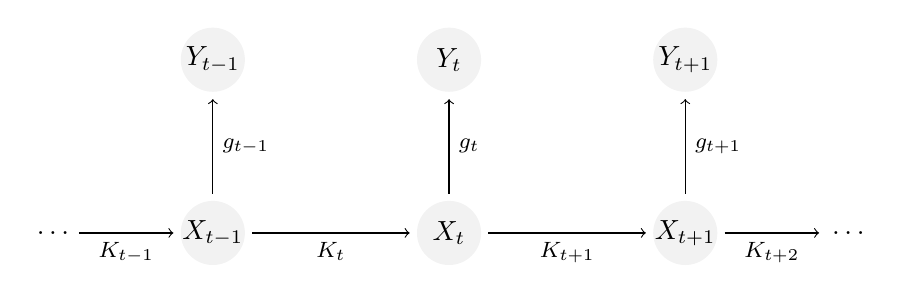
\begin{tikzpicture}
\filldraw[gray!10] (-3,0) circle (0.4);
\filldraw[gray!10] (-3,2.2) circle (0.4);
\filldraw[gray!10] (0,0) circle (0.4);
\filldraw[gray!10] (0,2.2) circle (0.4);
\filldraw[gray!10] (3,0) circle (0.4);
\filldraw[gray!10] (3,2.2) circle (0.4);
\node at (3,2.2) {$Y_{t+1}$};
\node at (3,0) {$X_{t+1}$};
\node at (0,2.2) {$Y_{t}$};
\node at (0,0) {$X_{t}$};
\node at (-3,2.2) {$Y_{t-1}$};
\node at (-3,0) {$X_{t-1}$};
\node at (-5,0) {$\dots$};
\node at (5.1,0) {$\dots$};
\draw[->] (-4.7,0)-- node[anchor=north] {\footnotesize{$K_{t-1}$}} (-3.5,0);
\draw[->] (-2.5,0)-- node[anchor=north] {\footnotesize{$K_t$}} (-0.5,0);
\draw[->] (0.5,0)-- node[anchor=north] {\footnotesize{$K_{t+1}$}} (2.5,0);
\draw[->] (3.5,0)-- node[anchor=north] {\footnotesize{$K_{t+2}$}} (4.7,0); 
\draw[->] (-3,0.5)-- node[anchor=west] {\footnotesize{$g_{t-1}$}} (-3,1.7);
\draw[->] (0,0.5)-- node[anchor=west] {\footnotesize{$g_t$}} (0,1.7);
\draw[->] (3,0.5)-- node[anchor=west] {\footnotesize{$g_{t+1}$}} (3,1.7);
\end{tikzpicture}
\caption[State space model]{Conditional independence graph for a general state space model. $(X_t)$ is a Markov process with transition kernels $(K_t)$ representing the underlying state of the system. $Y_t$ is a noisy observation of $X_t$ for each $t$.}
\label{fig:SSM}
\end{figure}
The general model has two components: a Markov process $(X_t)_{t\in\mathbb{N}_0}$ representing the (unobservable) underlying state of the system, and a sequence $(Y_t)_{t\in\mathbb{N}_0}$ of observations containing information about the underlying state. The model is characterised by its conditional independence structure (Figure~\ref{fig:SSM}) along with an initial distribution $\mu$, the Markov ``transition'' kernels $(K_t)_{t\in\mathbb{N}}$ and the ``emission'' distributions $(g_t)_{t\in\mathbb{N}_0}$. 
Written as a hierarchical model,
\begin{align}
X_0 &\sim \mu(\cdot) & \notag\\
X_{t+1} \mid X_t &\sim K_{t+1}(\cdot | X_t) & \text{for } t=0, 1, \dots
        \label{eq:SSM_spec}\\
Y_t \mid X_t &\sim g_t(\cdot | X_t) & \text{for } t=0, 1, \dots \notag
\end{align}
The index $t$ will frequently be referred to as ``time'', since in many applications the sequence is indeed a time series, but it need not be.

Here $X$ and/or $Y$ may be multivariate and observation times need not be equally spaced. Straightforward generalisations of the stated model can allow for situations in which observations are not available as often as the state is updated (up to and including the extreme where the state is a continuous-time Markov process but the observations are available only at discrete times) or on the other hand where observations are made more frequently than the state is updated.

Applications include target tracking, where $X$ is the true position of some object and $Y$ encodes some measurements from sensors e.g.\ radar; stochastic volatility models, where $X$ is the volatility and $Y$ is the observed value e.g.\ the price of a stock; change-point detection; and many other situations in which there is an observed time series from which one would like to do inference or prediction.

The principal inferences of interest in state space models are:
\begin{description}
\item [filtering] $p(x_t\mid y_{0:t})$: inferring the current state $x_t$ from the observations up to now $y_{0:t}$
\item [prediction] $p(x_{t+h}\mid y_{0:t})$: inferring a future state $x_{t+h}$ from the observations up to now $y_{0:t}$
\item [(complete) smoothing] $p(x_{0:t}\mid y_{0:t})$: inferring the sequence of states up to now $x_{0:t}$ from the observations up to now $y_{0:t}$
\item [fixed-lag smoothing] $p(x_{t-h:t}\mid y_{0:t})$: inferring the last $h$ states $x_{t-h:t}$ from the observations up to now $y_{0:t}$
\end{description}
If the dynamics of the state space model are parametrised by some $\theta$, i.e.\ $g_t$ and/or $K_t$ depend on $\theta$, we may also be interested in parameter inference or computing the likelihood $p(y_{0:t})$ of the observed data for particular values of $\theta$. Such a model is considered in Section~\ref{sec:particleGibbs}.

In certain cases, these inference problems may be solved analytically (Section~\ref{sec:SSM_exact_inference}), but this is not typically the case. For intractable models we must resort to Monte Carlo methods. However, state space inference is problematic even with Monte Carlo. 
The main difficulties are that the dimension of the target distributions may increase along the sequence, and that there is strong dependence between consecutive distributions. Markov chain Monte Carlo (MCMC), for instance, is known to struggle with highly correlated targets\seb{[citation]} and its performance drops drastically as dimension increases, despite convergence rates that are supposedly independent of dimension\seb{[citation]}.

As we will see in Section~\ref{sec:SMC_FK}, sequential Monte Carlo overcomes these problems, turning the problematic properties of the target distribution to its benefit. Correlation between consecutive targets is exploited for sequential updating, which is able to handle the incrementing dimensionality. The resulting linear-in-$t$ computational complexity also allows inference to be performed on-line, that is, updating the posterior distribution(s) as observations arrive.




\subsection{Exact inference in state space models}
\label{sec:SSM_exact_inference}
If the state space model has linear dynamics with Gaussian errors, the posterior distributions of interest are also Gaussian. The posterior mean and covariance satisfy certain recursions, implemented by the Kalman filter \parencite{kalman1960} and Rauch-Tung-Striebel smoother \parencite{rauch1965}. 
Recursions are also available for some other conjugate models: see for example \textcite{vidoni1999}.
Another analytic case occurs if the state space $\mathcal{X}$ is finite, in which case any integrals become finite sums, and the forward-backward algorithm \parencite{baum1970} yields the exact posteriors. However, if the state space becomes large, albeit finite, exact computation becomes infeasible.

If the model is Gaussian but non-linear, the posterior filtering distributions can be estimated using the \emph{extended Kalman filter} (see for example \textcite{jazwinski2007}), which applies a first-order approximation in order to make use of the Kalman filter. This method performs well on models that are ``almost linear''. The resulting predictor is only \emph{optimal} when the model is actually linear, in which case the extended Kalman filter coincides with the Kalman filter.

For models that are high-dimensional or highly non-linear or for which gradients are not readily available, the exact Kalman filter updates can be replaced by sample approximations.
The \emph{ensemble Kalman filter} \parencite{evensen1994} uses a Monte Carlo sample from the current time, propagates these points through the transition dynamics, and uses the sample covariance as an estimator of the updated covariance matrix. The means (which are cheaper to evaluate and more stable than the covariances) are still updated using the Kalman filter recursion, based on the estimated covariance.
The \emph{unscented Kalman filter} \parencite{wan2000} uses a deterministic sample chosen via the \emph{unscented transformation}, which is then propagated through the non-linear transition kernel to obtain a characterisation of the distribution at the next time step. The sample consists of $2d+1$ points, where $d$ is the dimension of the state space, and defines a Gaussian approximation to the updated distribution. If the model is really linear-Gaussian then the sample points are sufficient to recover the correct distribution.

In complex or high-dimensional models, such techniques may not be feasible, in which case we must resort to Monte Carlo methods.
Markov chain Monte Carlo performs woefully on state space models due to the high dimension of the parameter space and high correlation between dimensions. 
But we can exploit the sequential nature of the underlying dynamics to decompose the problem into a sequence of inferences of fixed dimension.
This is the motivation behind sequential Monte Carlo (SMC).


\subsection{Feynman-Kac models}
\label{sec:FKmodels}
\seb{Give example of non-SSM that is FK? Obvious options are SMC samplers e.g.\ for rare event simulation or sequential ABC or tempering.}\\
State space models are very natural and intuitive applications, but they do not do justice to the scope of SMC algorithms, which is much wider.
On the other hand, 
%the \emph{Feynman-Kac} formalism captures the full scope, since 
every SMC algorithm is a Monte Carlo approximation of some \emph{Feynman-Kac} model.
Before formally introducing SMC let us therefore define a generic Feynman-Kac model.
For a more in-depth study, the reader is directed to the exhaustive books by \textcite{delmoral2004, delmoral2013} or the more accessible \textcite[Chapter 5]{chopin2020}.

Define a state space $\mathcal{X}$ and a time horizon $T$. In this presentation we assume that the state space $\mathcal{X}$ is common for all times: this is often not the case in practice, but the generalisation to a sequence of state spaces is straightforward.
The basic components of the Feynman-Kac model are a Markov law, defined by an initial distribution $\mathbb{M}_0$ on $\mathcal{X}$ and transition kernels $M_t: \mathcal{X} \mapsto \mathcal{X}$ for $t=1,\dots,T$; and a sequence of ``potential'' functions $G_0 : \mathcal{X} \mapsto [0,\infty)$  and $G_t : \mathcal{X}^2 \mapsto [0,\infty)$ for $t=1,\dots,T$.
From these we construct a sequence of Feynman-Kac measures $(\mathbb{Q}_t)_{t=0:T}$ defined by the changes of measure
\begin{equation}
\mathbb{Q}_t (dx_{0:T}) = \frac{1}{L_t} G_0(x_0) \mathbb{M}_0(dx_0)
        \left\{ \prod_{s=1}^t G_s(x_{s-1}, x_s) \right\} 
        \left\{ \prod_{s=1}^T M_s(x_{s-1}, dx_s) \right\} , \label{eq:FKmeasure}
\end{equation}
where $L_t$ is the normalising constant required to make $\mathbb{Q}_t$ a probability measure. Other quantities such as $\mathbb{Q}_t (dx_{0:t})$ can be obtained as marginals of \eqref{eq:FKmeasure}, allowing us to treat all of the inference problems described in Section~\ref{sec:SSMs} by approximating $\mathbb{Q}_t$ and then possibly marginalising.

The generic state space model introduced in \eqref{eq:SSM_spec} may be described by a Feynman-Kac model where:
\begin{align}
\mathbb{M}_0 &:= \mu \notag\\
M_t (x_{t-1}, dx_t) &:= K_t (dx_t \mid x_{t-1}) & \text{for } t=1,\dots,T \notag\\
G_0 (x_0) &:= g_0 ( y_0 \mid x_0 ) \notag\\
G_t (x_{t-1}, x_t) &:= g_t( y_t \mid x_t ) & \text{for } t=1,\dots,T . \label{eq:bootstrapFK}
\end{align}
This is not the only Feynman-Kac model for \eqref{eq:SSM_spec}; this corresponds to the ``bootstrap'' SMC algorithm, which is the simplest implementation but may be significantly outperformed by more involved algorithms such as ``guided''\seb{[citation]} and ``auxiliary'' \parencite{pitt1999, carpenter1999} variants. Feynman-Kac formalisms for these variants are presented for example in \textcite[Section 5.1.2]{chopin2020}.
\seb{Say something about the time horizon, which we have now fixed, but was infinite in SSMs section.}

It remains to demonstrate that the measures $\mathbb{Q}_t$ arising from \eqref{eq:bootstrapFK} are sufficient for all the usual inference problems in the corresponding state space model \eqref{eq:SSM_spec}.
By construction, the complete smoothing distribution is precisely
\begin{align*}
\mathbb{Q}_t (dx_{0:t})
&= \frac{1}{L_t} G_0(x_0) \mathbb{M}_0(dx_0)
        \prod_{s=1}^t G_s(x_{s-1}, x_s) M_s(x_{s-1}, dx_s) \\
&= g_0(y_0 \mid x_0) \mu(dx_0) 
        \prod_{s=1}^t g_s(y_s \mid x_s) K_s(dx_s \mid x_{s-1}) \\
&= p(dx_{0:t} \mid y_{0:t}) .
\end{align*}
The filtering, prediction and fixed-lag smoothing distributions are all also marginals of $\mathbb{Q}_t(dx_{0:T})$:
\begin{align*}
p(dx_t \mid y_{0:t}) &= \mathbb{Q}_t (dx_t) \\
p(dx_{t+h} \mid y_{0:t}) &= \mathbb{Q}_t (dx_{t+h}) \\
p(dx_{t-h:t} \mid y_{0:t}) &= \mathbb{Q}_t (dx_{t-h:t}) ,
\end{align*}
while the likelihood $p(y_{0:t}) = L_t$.
The upshot of this is that if we have access to a Monte Carlo approximation of $\mathbb{Q}_t(dx_{0:T})$ then we can conduct inference on any of these distributions, since marginalisation of Monte Carlo samples is trivial. The likelihood, on the other hand, is not obtained by marginalisation; nevertheless, we will see that approximations of the likelihood can also be obtained ``for free''. 
The next section describes how we may obtain Monte Carlo samples from $\mathbb{Q}_t(dx_{0:T})$.




\subsection{Sequential Monte Carlo for Feynman-Kac models}
\label{sec:SMC_FK}
In order to implement the SMC algorithm corresponding to a given Feynman-Kac model, we need to be able to sample from $\mathbb{M}_0$ and from $M_t(x, \cdot)$ for all $x,t$; and evaluate $G_t(x, y)$ pointwise for each $x,y, t$.
Under these conditions we may implement Algorithm~\ref{alg:SMC}, which describes a generic SMC algorithm. 
The only free choices are the parameter $N$ which dictates the number of ``particles'' used, and the \textsc{resample} procedure.
However, remember that given a particular state space model there is also a choice of possible Feynman-Kac descriptions, and this choice can strongly affect performance.

\begin{algorithm}[ht]
\vspace*{10pt}
\DontPrintSemicolon
\KwIn{$T, N, \mathbb{M}_0, (M_t)_{t=1}^T, (G_t)_{t=0}^T$}
\lFor{$i \in \{1,\dots,N\}$}{ 
	Sample $X_0^{(i)} \sim \mathbb{M}_0(\cdot)$
}
\lFor{$i \in \{1,\dots, N\}$}{
		$w_{0}^{(i)} \gets  \left\{{\sum_{j=1}^N G_0(X_0^{(j)})}\right\}^{-1}{G_0(X_0^{(i)})} $ 
	}
\For{$t \in \{1,\dots, T\}$}{
	Sample $a_{t-1}^{(1:N)} \sim $ \textsc{resample}$(\{1,\dots ,N\}, w_{t-1}^{(1:N)}$)\;
	\lFor{$i \in \{1,\dots,N\}$}{
		Sample $X_{t}^{(i)} \sim M_{t}(X_{t-1}^{(a_{t-1}^{(i)})}, \cdot)$
	}
	\lFor{$i \in \{1,\dots, N\}$}{	
		$w_{t}^{(i)} \gets \Big\{ {\sum_{j=1}^N G_{t}(X_{t-1}^{(a_{t-1}^{(j)})}, X_{t}^{(j)}) }\Big\}^{-1} G_{t}(X_{t-1}^{(a_{t-1}^{(i)})},X_{t}^{(i)}) $
	}
}
\vspace*{10pt}
\caption{Sequential Monte Carlo for a generic Feynman-Kac model}
\label{alg:SMC}
\end{algorithm}

The choice of \textsc{resample} procedure can also have a profound effect on performance and is discussed in detail in Section~\ref{sec:resampling}. 
Resampling is not necessary for the algorithm to be valid, but it is important to ensure good performance. Its purpose is to periodically ``reset'' the weights $w_t^{(1:N)}$, preventing \emph{weight degeneracy}. This is the phenomenon that multiplying importance weights over time causes the variance of the weights to increase exponentially, until after some iterations practically all of the weight is concentrated on one particle, with the rest having weights very close to zero. This means that the Monte Carlo sample (of size $N$) essentially consists of just one sample, so that the Monte Carlo approximations have very high variance.

The idea of resampling is to make multiple copies of particles with high weights and eliminate particles with low weights, then reset the weights to $w_t^{(1:N)} = (1,\dots,1)/N$. Done correctly, this procedure does not introduce any bias and, although it increases variance in the short term by adding extra randomness, it improves stability in the long term.
It also prevents computational budget being ``wasted'' on simulating low-weight particles which do not contribute much to the approximation.

For each $i=1,\dots,N$, the \textsc{resample} procedure selects a \emph{parent}, indexed by $a_{t-1}^{(i)} \in \{1,\dots,N\}$, which copies its state to the $i$th particle in the next iteration. These copies are then mutated independently and so the algorithm goes on.
We define the \emph{offspring counts} for each $i,t$ as
\begin{equation*}
\nu_{t-1}^{(i)} := |\{ j: a_{t-1}^{(j)} = i \}| ,
\end{equation*}
the number of copies in generation $t+1$ of particle $i$ from generation $t$ appearing by resampling. Notice that $\nu_t^{(1:N)}$ is expressed as a non-injective function of $a_t^{(1:N)}$, and as such carries less information.
To ensure Algorithm~\ref{alg:SMC} is valid, we assume that the resampling procedure satisfies the following properties: that the population size $N$ is conserved; and that, given $w_{t-1}^{(1:N)}$, the expectation of $\nu_{t-1}^{(i)}$ is proportional to $w_{t-1}^{(i)}$ for each $i$.
The latter property is known as \emph{unbiasedness}.
These requirements are made rigorous in Definition~\ref{defn:resampling}.

\begin{figure}[ht]
\centering
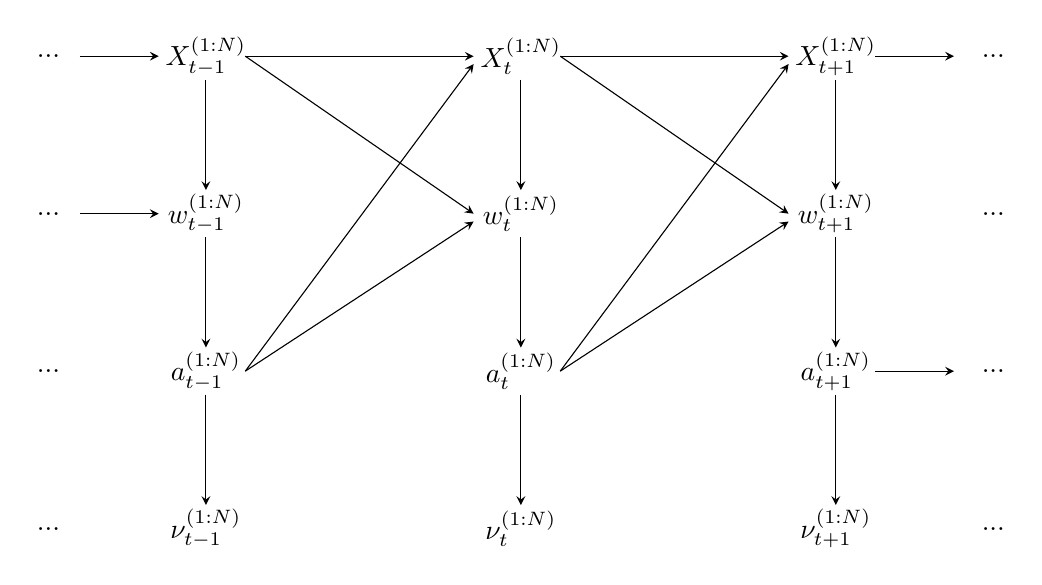
\begin{tikzpicture}[>=stealth]
% left dots
\node at (-2,0) {...};
\node at (-2,-2) {...};
\node at (-2,-4) {...};
\node at (-2,-6) {...};
% labels (t+1)
\node at (0,0) {$X_{t-1}^{(1:N)}$};
\node at (0,-2) {$w_{t-1}^{(1:N)}$};
\node at (0,-4) {$a_{t-1}^{(1:N)}$};
\node at (0,-6) {$\nu_{t-1}^{(1:N)}$};
% labels t
\node at (4,0) {$X_{t}^{(1:N)}$};
\node at (4,-2) {$w_{t}^{(1:N)}$};
\node at (4,-4) {$a_{t}^{(1:N)}$};
\node at (4,-6) {$\nu_{t}^{(1:N)}$};
% labels (t-1)
\node at (8,0) {$X_{t+1}^{(1:N)}$};
\node at (8,-2) {$w_{t+1}^{(1:N)}$};
\node at (8,-4) {$a_{t+1}^{(1:N)}$};
\node at (8,-6) {$\nu_{t+1}^{(1:N)}$};
% right dots
\node at (10,0) {...};
\node at (10,-2) {...};
\node at (10,-4) {...};
\node at (10,-6) {...};
% arrows (t+1) -> t
\draw[->] (0.5,0)--(3.4,0);
\draw[->] (0.5,0)--(3.4,-2);
\draw[->] (0.5,-4)--(3.4,-2.1);
\draw[->] (0.5,-4)--(3.4,-0.1);
% arrows t -> (t-1)
\draw[->] (4.5,0)--(7.4,0);
\draw[->] (4.5,0)--(7.4,-2);
\draw[->] (4.5,-4)--(7.4,-2.1);
\draw[->] (4.5,-4)--(7.4,-0.1);
% vertical arrows (t+1)
\draw[->] (0,-0.3)--(0,-1.7);
\draw[->] (0,-2.3)--(0,-3.7);
\draw[->] (0,-4.3)--(0,-5.7);
% vertical arrows t
\draw[->] (4,-0.3)--(4,-1.7);
\draw[->] (4,-2.3)--(4,-3.7);
\draw[->] (4,-4.3)--(4,-5.7);
% vertical arrows (t-1)
\draw[->] (8,-0.3)--(8,-1.7);
\draw[->] (8,-2.3)--(8,-3.7);
\draw[->] (8,-4.3)--(8,-5.7);
% arrows ... -> t+1
\draw[->] (-1.6,0)--(-0.6,0);
\draw[->] (-1.6,-2)--(-0.6,-2);
% arrows t-1 -> ...
\draw[->] (8.5,0)--(9.5,0);
\draw[->] (8.5,-4)--(9.5,-4);
\end{tikzpicture}
\caption[Conditional dependence structure of SMC algorithm]{Part of the conditional dependence graph implied by Algorithm~\ref{alg:SMC}. The direction of time is from left to right.}
\label{fig:cond_indep_graph}
\end{figure}
%\vspace{10pt}
%\begin{algorithm}
%\DontPrintSemicolon
%\KwData{$N, T, \mu, (K_t)_{t=1}^T, (g_t)_{t=0}^T$}
%\lFor{$i \in \{1,\dots,N\}$}{ 
%	Sample $X_0^{(i)} \sim \mu(\cdot)$
%}
%\lFor{$i \in \{1,\dots, N\}$}{
%		$w_{0}^{(i)} \gets  \left\{{\sum_{j=1}^N g_0(X_0^{(j)})}\right\}^{-1}{g_0(X_0^{(i)})} $ 
%	}
%\For{$t \in \{0,\dots, T-1\}$}{
%	Sample $a_t^{(1:N)} \sim $ \textsc{resample}$(\{1,\dots ,N\}, w_t^{(1:N)}$)\;
%	\lFor{$i \in \{1,\dots,N\}$}{
%		Sample $X_{t+1}^{(i)} \sim K_{t+1}(X_t^{(a_t^{(i)})}, \cdot)$
%	}
%	\lFor{$i \in \{1,\dots, N\}$}{	
%		$w_{t+1}^{(i)} \gets \Big\{ {\sum_{j=1}^Ng_{t+1}(X_t^{(a_t^{(j)})},X_{t+1}^{(j)}) }\Big\}^{-1} g_{t+1}(X_t^{(a_t^{(i)})},X_{t+1}^{(i)}) $
%	}
%}
%\caption{Sequential Monte Carlo}\label{alg:SMC_SSM}
%\end{algorithm}
%\vspace{10pt}
Figure~\ref{fig:cond_indep_graph} shows a section of the conditional dependence graph implied by Algorithm~\ref{alg:SMC}.
Because the algorithm proceeds sequentially, with each iteration incorporating a constant amount of data, its computational cost is linear in the time horizon $T$. Furthermore, the bootstrap algorithm, where the Feynman-Kac model is \eqref{eq:bootstrapFK}, processes the data $y_{0:T}$ one observation at a time via $G_t(x_t) = g_t(y_t \mid x_t)$, which means that it can be run on-line, incorporating each observation as it becomes available.
This is in stark contrast to a standard MCMC approach, for example, which would have to process all of the data at once up to a fixed time horizon. Adding one more observation would require running the MCMC algorithm from scratch on the extended target, making the computational cost at least linear \emph{per time point} and rendering on-line inference infeasible.

The output of Algorithm~\ref{alg:SMC} is, for $i=1,\dots, N$ and $t=0,\dots,T$, the \emph{states} $X_t^{(i)} \in \mathcal{X}$, the \emph{weights} $w_t^{(i)} \in [0,1]$ and, for $i=1,\dots, N$ and $t=0,\dots,T-1$, the \emph{parental indices} $a_t^{(i)} \in \{1,\dots,N\}$.
Depending on the application, one may want to retain only a subset of this output in order to reduce memory usage.

The output can be used to construct discrete approximations of the various distributions of interest, with which one may estimate integrals against test functions, i.e.\ expectations.
The filtering distribution $p(x_t \mid y_{0:t})$ is approximated by the empirical measure
\begin{equation*}
\sum_{i=1}^N w_t^{(i)} \delta_{ X_t^{(i)} } ,
\end{equation*}
where $\delta_x$ denotes a unit mass at $x$.
That is, expectations of appropriate test functions $\varphi : \mathcal{X} \mapsto \mathbb{R}$ are approximated by their expectations with respect to the empirical measure,
\begin{equation*}
\E[ \varphi(x_t) \mid y_{0:t} ]
\simeq \sum_{i=1}^N w_t^{(i)} \varphi( X_t^{(i)} ) .
\end{equation*}
The precise meaning of approximation (or $\simeq$) is clarified in Section~\ref{sec:SMC_theory}.
To approximate the smoothing distribution, we first define the state \emph{trajectories} $X_{t,0:t}^{(i)}$ (for each $i \in \{1,\dots,N\}$) by setting $X_{t,t}^{(i)} := X_t^{(i)}$ and tracing back through the ancestors via the recursion $X_{t,s}{(i)} = X_{t,s+1}^{( a_t^{(i)} )}$ for each $s \in \{0,\dots, t\}$. 
We can then construct the approximation
\begin{equation*}
\sum_{i=1}^N w_t^{(i)} \delta_{ X_{t,0:t}^{(i)} } 
\end{equation*}
of the smoothing distribution $p(x_{0:t} \mid y_{0:t})$, with which we can calculate expectations as above.
Similar approximations can be constructed for prediction and fixed-lag smoothing.
%\seb{...be explicit or no?}.
We can also approximate the marginal likelihood using the \emph{unnormalised} weights:
%\seb{should I introduce notation e.g. $\tilde{w}$ for the unnormalised weights, and give them a separate line in Algorithm~\ref{alg:SMC}, and include them in the possible outputs of the algorithm?}
\begin{equation}\label{eq:likelihood_estimate}
L_t 
\simeq \frac{1}{N} \sum_{i=1}^N G_0(X_0^{(i)}) \prod_{t=1}^T \frac{1}{N}
        \sum_{i=1}^N G_t( X_{t-1}^{ a_{t-1}^{(i)} }, X_t^{(i)} ) .
\end{equation}
The unnormalised weights could be output directly from Algorithm~\ref{alg:SMC}, or re-calculated from the states as shown here.







\subsection{Theoretical justification}
\label{sec:SMC_theory}
It can be shown that SMC approximations of expectations of test functions satisfy various desirable properties. For instance, it is quite easy to show that the filtering approximations converge:
\begin{equation*}
\sum_{i=1}^N w_t^{(i)} \varphi( X_t^{(i)} ) 
\longrightarrow \mathbb{Q}_t(\varphi) ,
\end{equation*}
almost surely and in the $L_2$ sense, as $N\to\infty$, under some conditions.
Moreover, they satisfy a central limit theorem:
\begin{equation*}
\sqrt{N} \left( \sum_{i=1}^N w_t^{(i)} \varphi( X_t^{(i)} ) - \mathbb{Q}_t(\varphi) \right)
\longrightarrow  \N( 0, \sigma_t(\varphi) )
\end{equation*}
in distribution, as $N\to\infty$. 
The $\sqrt{N}$ scaling agrees with the standard convergence rate for Monte Carlo approximations.
Under additional conditions, the asymptotic variances $\sigma_t(\varphi)$ are stable over $t$, justifying the use of SMC filtering on-line.
It can also easily be shown that the likelihood estimates \eqref{eq:likelihood_estimate} are unbiased \parencite[see for example][Proposition 16.3]{chopin2020}.

There are many other results concerning convergence, stability and error bounds for SMC algorithms. A full exposition of these results and their conditions is beyond the scope of this work, but the book by \textcite{delmoral2013} provides an exhaustive treatment, and some of the key ideas and results are also developed in \textcite[Chapter 11]{chopin2020}.
Suffice it to say that SMC algorithms enjoy enough theoretical properties to be useful in practice.





\section{Coalescent theory}
\label{sec:coaltheory}
The current work draws on the literature around coalescent theory, primarily from population genetics. This section summarises the relevant parts of that literature. We will see in Section~\ref{sec:SMC_genealogies} how it applies to SMC.

\subsection{Kingman's coalescent}
The Kingman coalescent \parencite{kingman1982gene, kingman1982coal, kingman1982exch} is a continuous-time Markov process on the space of partitions of $\mathbb{N}$. For our purposes we need only consider its restriction to $\{1,\dots,n\}$, termed the $n$-coalescent (Definition~\ref{def:kingman}), since we only ever consider finite samples from a population. 
%However, an excellent probabilistic introduction to the Kingman coalescent from the point-of-view of exchangeable random partitions can be found in \textcite[Chapters 1--2]{berestycki2009}. \seb{or \textcite{wakeley2009} ? or \textcite{durrett2008} ?}
\begin{defn}%[Kingman's $n$-coalescent]
\label{def:kingman}
Let $\mathcal{P}_n$ denote the set of partitions of $\{1,\dots,n\}$.
The \emph{$n$-coalescent} is the homogeneous continuous-time Markov process on $\mathcal{P}_n$ with infinitesimal generator $Q$ having entries
\begin{equation}\label{eq:KCgenerator}
q_{\xi,\eta} = \begin{cases}
1 & \xi \prec \eta\\
-|\xi|(|\xi|-1)/2 & \xi=\eta \\
0 & \text{otherwise}
\end{cases}
\end{equation}
for every $\xi, \eta \in \mathcal{P}_n$, where $|\xi|$ denotes the number of blocks in $\xi$, and $\xi \prec \eta$ means that $\eta$ is obtained from $\xi$ by merging exactly one pair of blocks.
\end{defn}
\begin{figure}
\centering
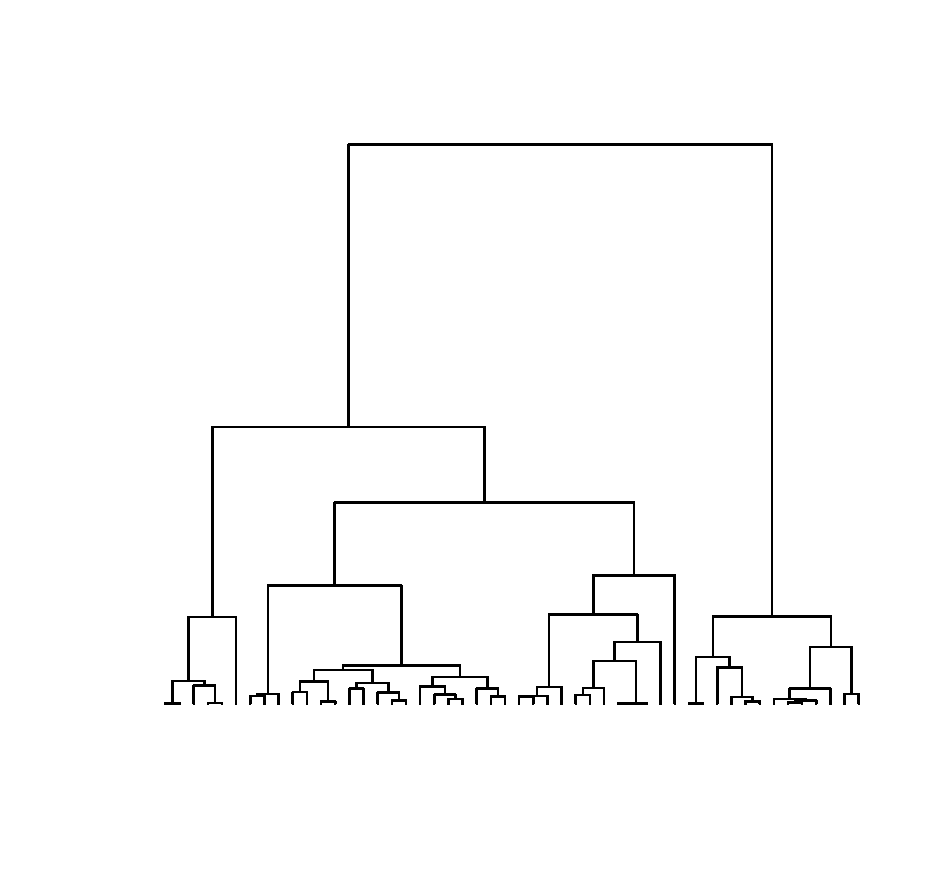
\includegraphics[width=0.6\textwidth, trim={2.8cm 3cm 1.5cm 2cm}, clip]{../plots/ncoalescent.pdf}
\caption[The $n$-coalescent]{A realisation of the $n$-coalescent with $n=50$.}
\end{figure}
A particularly attractive feature of the $n$-coalescent is its tractability; its distribution and those of many statistics of interest are available in closed form (Section \ref{sec:KCproperties}).
It turns out also to be extremely useful as a limiting distribution in population genetics, including in its domain of attraction the genealogies of a wide range of population models (Section \ref{sec:popgenmodels}).


\subsection{Properties of Kingman's coalescent}\label{sec:KCproperties}
\seb{Refer to more exhaustive studies of the properties in the literature, e.g.\ \textcite[Section 1.2]{durrett2008}.}\\
The simplicity of $Q$ allows various properties of the $n$-coalescent to be studied analytically.
Starting with $n$ blocks, exactly $n-1$ coalescences are required to reach the absorbing state where all blocks have coalesced, known in population genetics as the \emph{most recent common ancestor} (MRCA).

\begin{figure}[ht]
\centering
\begin{tikzpicture}
% horizontal lines
\draw[dotted, gray] (-0.5,-1)--(6,-1);
\draw[dotted, gray] (-0.5,-0.2)--(6,-0.2);
\draw[dotted, gray] (-0.5,0.5)--(6,0.5);
\draw[dotted, gray] (-0.5,1.3)--(6,1.3);
\draw[dotted, gray] (-0.5,3.3)--(6,3.3);

% tree
\draw[thick] (0,-1)--(0,-0.2);
\draw[thick] (1,-1)--(1,-0.2);
\draw[thick] (0,-0.2)--(1,-0.2);
\draw[thick] (0.5,-0.2)--(0.5,1.3);
\draw[thick] (2,-1)--(2,1.3);
\draw[thick] (0.5,1.3)--(2,1.3);
\draw[thick] (3,-1)--(3,0.5);
\draw[thick] (4,-1)--(4,0.5);
\draw[thick] (3,0.5)--(4,0.5);
\draw[thick] (1.25,1.3)--(1.25,3.3);
\draw[thick] (3.5,0.5)--(3.5,3.3);
\draw[thick] (1.25,3.3)--(3.5,3.3);

% interval arrows
\draw[<->] (5,-1)--(5,-0.2);
\draw[<->] (5,-0.2)--(5,0.5);
\draw[<->] (5,0.5)--(5,1.3);
\draw[<->] (5,1.3)--(5,3.3);

% small t's
\node at (5.2, -0.6) {\footnotesize{$t_5$}};
\node at (5.2, 0.15) {\footnotesize{$t_4$}};
\node at (5.2, 0.9) {\footnotesize{$t_3$}};
\node at (5.2, 2.3) {\footnotesize{$t_2$}};

% capital T's
\node[anchor=west] at (6, -1) {\footnotesize{$T_5 = 0$}};
\node[anchor=west] at (6, -0.2) {\footnotesize{$T_4$}};
\node[anchor=west] at (6, 0.5) {\footnotesize{$T_3$}};
\node[anchor=west] at (6, 1.3) {\footnotesize{$T_2$}};
\node[anchor=west] at (6, 3.3) {\footnotesize{$T_1 = T_{MRCA}$}};
\end{tikzpicture}
\caption{Definitions of $t_i$, $T_i$ in the $n$-coalescent.}
\label{fig:KC_timedefns}
\end{figure}

Denote by $t_2, \dots, t_n$ the waiting times between coalescent events, where $t_i$ is the amount of time for which the coalescent has exactly $i$ distinct lineages (see Figure~\ref{fig:KC_timedefns}).
A consequence of Definition~\ref{def:kingman} is that these waiting times are independent and have distributions
\begin{equation*}
t_i \sim \Exp\left( \binom{i}{2} \right) .
\end{equation*}
The partial sum $T_k := \sum_{i=k+1}^n t_i$ gives the total time up to the $(n-k)^{th}$ coalescence event, that is, the first time at which there are only $k$ lineages remaining out of the initial $n$ (see Figure~\ref{fig:KC_timedefns}).
The partial sums, being sums of independent Exponential random variables, have HyperExponential distributions.

Another important property of the $n$-coalescent is \emph{exchangeability}. That is, its law is invariant under permutations of the branches. This can be seen from \eqref{eq:KCgenerator} since the merge rate is equal for every pair of partitions $\xi \prec \eta$.
%\seb{Refer back to the following three properties later on with reference to their relevance in SMC.}

\subsubsection{Time to MRCA}
Of particular interest is the tree height or time to the most recent common ancestor, $T_{MRCA} := T_1$.
With some algebra we find, for instance,
\begin{equation*}
\E[ T_{MRCA} ] 
= \sum_{i=2}^{n} \E[t_i]
= \sum_{i=2}^n \frac{2}{i(i-1)}
= 2 \sum_{i=2}^n \left\{ \frac{1}{i-1} - \frac{1}{i} \right\}
= 2 \left( 1 - \frac{1}{n} \right)
\end{equation*}
and
\begin{equation*}
\V[ T_{MRCA} ] 
= \sum_{i=2}^n \V[t_i]
= \sum_{i=2}^n \left( \frac{2}{i(i-1)} \right)^2 .
\end{equation*}
The expected tree height converges to 2 as $n\to\infty$, and the variance converges to $4(\pi^2 - 9)/3 \simeq 1.16$.
The somewhat surprising fact that the tree height does not diverge with $n$ is a result of the very high rate of coalescence close to the bottom of the tree. This rate is large enough that the full Kingman coalescent (on $\mathbb{N}$) \emph{comes down from infinity}, that is, despite starting with infinitely many blocks, after any positive amount of time these have coalesced into finitely many blocks.
%\seb{Plot mean with sd-ribbon over $n$ for an illustration? SD ribbon isn't the right thing; since we apparently know the actual distribution, plot a high density interval of that. (also for $L$)}


\subsubsection{Total branch length}
Another quantity of interest is the total branch length,
$ L := \sum_{i=2}^n i t_i $.
For instance
\begin{equation*}
\E[ L ] 
= \sum_{i=2}^n i \E[ t_i ]
= \sum_{i=2}^n \frac{2}{i-1}
= \sum_{i=1}^{n-1} \frac{2}{i} %,
\simeq 2 \ln(n-1) 
\end{equation*}
%a harmonic series, 
and
\begin{equation*}
\V[ L ] 
= \sum_{i=2}^n i^2 \V[ t_i ]
= \sum_{i=2}^n \frac{4}{(i-1)^2}
= \sum_{i=1}^{n-1} \frac{4}{i^2} .
\end{equation*}
Note that although the mean total branch length diverges with $n$, the variance converges to a constant, $4\pi^2 /6 \simeq 6.58$.


\subsubsection{Probability that sample MRCA is population MRCA}
One other interesting quantity is the probability that the MRCA of $k$ random lineages coincides with the population MRCA \parencite[e.g.][Theorem 1.7]{durrett2008}.
Consider a random subsample of size $k$ among $n$ lineages distributed according to the $n$-coalescent.
Denote by $S_{k,n}$ the event that these $k$ lineages have the same MRCA as all $n$ lineages.
The probability of this event is calculated in \textcite[Example 1]{saunders1984} and again in \textcite[Equation (3)]{spouge2014}, in both cases arising as a special case of more general results. A direct proof is given below.
%Denote by $S_k$ the relevant event: that a random sample of size $k$ among $N$ lineages has the same MRCA as the population.

Consider the two subtrees produced by cutting the full population tree just below the population MRCA. The $k$ sampled lineages coalesce before the full-sample MRCA if and only if all $k$ sampled leaves lie in just one of these two subtrees.
Let $X$ be the number of leaves in the left subtree, so $X \in \{1,\dots,n-1\} $, and a consequence of the exchangeability of the $n$-coalescent is that $X$ is uniformly distributed on that set.
Conditional on $X$ we have
\begin{equation*}
\Prob [S_{k,n}^c \mid X=x]
= \left[ \binom{x}{k} + \binom{n-x}{k} \right] \binom{n}{k}^{-1} .
\end{equation*}
Integrating against the distribution of $X$ gives
\begin{align*}
\Prob[ S_{k,n} ]
&= 1 - \frac{1}{n-1} \binom{n}{k}^{-1} \, \sum_{x=1}^{n-1} 
        \left[ \binom{x}{k} + \binom{n-x}{k} \right] \\
&= 1 - \frac{1}{n-1} \binom{n}{k}^{-1} 
        \left[ \binom{n}{k+1} + \binom{n}{k+1} \right] \\
&= \frac{k-1}{k+1} \frac{n+1}{n-1}
\end{align*}
using binomial identities and some algebra.
In particular, when $k=2$ we have
\begin{equation*}
\Prob[ S_{2,n} ]
=\frac{n+1}{3(n-1)} 
\end{equation*}
as the probability that a randomly chosen pair of lineages does not coalesce until the population MRCA.
%, in the limit $N\to\infty$, the proportion of leaves in the left subtree is uniformly distributed on $[0,1]$.
%Calling this proportion $X$, we have
%\begin{equation*}
%\Prob [ S_k^c \mid X=x]
%= x^k + (1-x)^k
%\end{equation*}
%Integrating against the distribution of $X$, the probability of interest is
%\begin{equation*}
%\Prob[ S_k ]
%= 1- \int_0^1 [ x^k + (1-x)^k ] dx
%= \frac{k-1}{k+1}
%\end{equation*}
%as required.
%
%The above is based on properties of the full Kingman coalescent, but similar results are available for the $n$-coalescent.
%Consider now a subsample of size $k$ among $n$ lineages that follow the $n$-coalescent.
%Denote by $S_{k,n}$ the event that these $k$ lineages have the same MRCA as all $n$ lineages.
%This probability of this event is calculated in \textcite[Example 1]{saunders1984} and again in \textcite[Equation (3)]{spouge2014}, in both cases arising as a special case of more general results. A direct proof is given below.
%
%Let $X$ be the number of leaves in the left subtree. So $X \in \{1,\dots,n-1\} $ and, like before, a consequence of exchangeability is that $X$ is uniformly distributed on that set.
%Now that the total number of branches is finite, we have to count more carefully. 
%As $n\to\infty$ this agrees with the population-level result above.



\subsection{Models in population genetics}\label{sec:popgenmodels}
The Kingman coalescent is the limiting coalescent process (in the large population limit) for a surprisingly wide range of population models. Some important examples of models in this ``domain of attraction'' are introduced in this section.
Common to all of these models are the following assumptions:
\begin{itemize}
\item The population has constant size $N$
\item Reproduction happens in discrete generations
\item The mechanism for assigning offspring to parents is identical at each generation, and independent between generations
\item The offspring distribution is exchangeable.
\end{itemize}
As in Section~\ref{sec:SMC_FK}, we define offspring counts in terms of parental indices as $\nu_j := |\{ i: a_i = j\}|$.
Since the assignment of offsrping to parents is i.i.d.\ across generations, there is no dependence on $t$.
Also, under the assumption of exchangeability, it is sufficient to consider only the offspring counts, rather than the parental indices (which generally carry more information).
%\seb{Crucially, in the neutral case, offspring counts carry all the information about the distribution of the genealogy that is contained in the parental indices.}
These models are all \emph{neutral}, that is exhibiting no natural selection, because the offspring counts at each generation are independent, so there can be no preferential propagation of certain ``fitter'' lineages.




\subsubsection{Cannings model}
The neutral Cannings model \parencite{cannings1974, cannings1975} is a general class which encompasses some other important models as special cases.

The Cannings model does not specify a particular distribution for the offspring counts; it just requires that the distribution is exchangeable, i.i.d.\ between generations, and preserves the population size. In particular, the probability of observing offspring counts $(v_1, \dots, v_N)$ must be invariant under permutations of this vector.

Rescaled genealogies of the neutral Cannings model converge to the Kingman coalescent as $N\to\infty$, under some conditions on the moments of the offspring distribution. 
For example, one may apply the sufficient conditions of \textcite{kingman1982gene}:
if $\V[\nu_1] \to \sigma^2 \in (0,\infty)$ and $\E[\nu_1^k]$ is bounded for all $k\in\mathbb{N}$ then, under the time scaling $N\sigma^{-2}$, the genealogies of the neutral Cannings model converge to the Kingman coalescent.
%\parencite[see for example][Section 2.2]{etheridge2011}. \seb{original reference for this? is not any Kingman 1982 papers, and certainly not Cannings 1974/5 which predates KC}




\subsubsection{Wright-Fisher model}
The neutral Wright-Fisher model \parencite{fisher1923, fisher1930, wright1931} is one of the most studied models in population genetics.
At each generation the existing population dies and is replaced by $N$ offspring. The offspring descend from parents $(a_1, \dots, a_N)$ which are selected according to
\begin{equation*}
a_i \overset{iid}{\sim} \Cat(\{1, \dots, N\}, (1/N, \dots, 1/N)).
\end{equation*}
The joint distribution of the offspring counts is therefore
\begin{equation*}
(v_1,\dots, v_N) \sim \Mn(N, (1/N, \dots, 1/N)).
\end{equation*}
Since the Multinomial distribution is exchangeable, the Wright-Fisher model is a special case of the Cannings model.
%There are several non-neutral variants of the Wright-Fisher model \seb{citations?}, but they are typically much less tractable than the neutral one.

\textcite{kingman1982gene} showed that the Wright-Fisher model satisfies his sufficient conditions, and thus the resulting genealogies, appropriately rescaled, converge to the Kingman coalescent as $N\to\infty$.
The correct time scale in this instance is $N$, since
\begin{equation*}
\V[\nu_1] = N\frac{1}{N} \left
(1 - \frac{1}{N}\right)
=\frac{N-1}{N}
\to 1 
=: \sigma^2 ,
\end{equation*}
so $N\sigma^{-2} = N$.



\subsubsection{Moran model}
The neutral Moran model \parencite{moran1958}, while perhaps less biologically relevant, is mathematically appealing because its simple dynamics make it particularly tractable.

At each generation, an ordered pair of individuals is selected uniformly at random. The first individual in this pair dies (i.e.\ leaves no offspring in the next generation), while the other reproduces (leaving two offspring). All of the other individuals leave exactly one offspring.
This is another special case of the neutral Cannings model, where the offspring distribution is now uniform over all permutations of $(0,2,1,1,\dots,1)$.

Under a suitable time-scaling, its genealogies converge to the Kingman coalescent\seb{[citation]}, although the sufficient conditions of \textcite{kingman1982gene} do not apply:
\begin{align*}
\V[\nu_1] 
&= \E[\nu_1^2] - \E[\nu_1]^2
= (0 + 1 \cdot \frac{N-2}{N} + 4 \cdot \frac{1}{N}) - (0 + 1 \cdot \frac{N-2}{N} + 2 \cdot \frac{1}{N})^2 \\
&= \frac{N+2}{N} - 1^2
= \frac{2}{N}
\to 0 ,
\end{align*}
violating the condition that $\sigma^2 >0$. 
However, that condition turns out not to be necessary \seb{[citation]}, and $\V[\nu_1]$ gives us the correct time scale on which to recover the Kingman coalescent: $N(\V[\nu_1])^{-1} = N^2/2$.
It is not surprising that the time scale is an order bigger than in the Wright-Fisher model, because the Moran model has a reproduction rate $O(N)$ times lower than in the Wright-Fisher model: at each generation $2$ individuals are involved in reproduction, as opposed to $N$ in the Wright-Fisher model.
%\seb{also cite a Moran-specific convergence result: not sure where (it isn't in Kingman 1982* or in Moran 1958 which predates KC)}




\subsection{Other convergence results}
\label{sec:previousgeneconv}
The original work of \textcite{kingman1982gene} provides sufficient conditions for the finite-dimensional distributions of genealogies of Cannings models to converge to those of the Kingman coalescent.
\textcite{mohle1998} provides another set of sufficient conditions which apply to the wider class of models in which the population size may vary deterministically, the offspring distributions are independent but not identical across generations, and exchangeability is replaced by the weaker \emph{random assignment} condition. 
For that class of models under the same conditions, \textcite{mohle1999} proved that the genealogies converge weakly as well as in the sense of finite-dimensional distributions.
\textcite{mohle2000} gives a simpler condition which is necessary and sufficient for convergence of Cannings genealogies to the Kingman coalescent. % that N&S condition is the exchangeable version of our main theorem condition.

Meanwhile many similar results were established for models in which the limiting process is not the Kingman coalescent.
Relaxing the conditions to allow multiple mergers in the limit admits $\Lambda$-coalescents as limiting processes, with the Kingman coalescent as a special case \parencite{pitman1999, sagitov1999, mohlesagitov1998}.
If simultaneous mergers are also allowed, the limiting process is in the even more general class of $\Xi$-coalescents \parencite{mohle2001}, and this class encompasses all possible limiting genealogies of Cannings models.

The focus of the current work is on systems that admit Kingman genealogies in the limit, among a wider class of models where, like \textcite{mohle1998, mohle1999}, exchangeability is relaxed to random assignment, and we also do not require independence between generations, so our models are not neutral. 
%In particular, this class of models is non-neutral.
Our main condition for convergence to the Kingman coalescent, which is introduced in Chapter~\ref{ch:limits}, can be considered a non-exchangeable non-neutral analogue of the condition presented in \textcite{mohle2000}.




\subsection{Particle populations}
Much of the population genetics framework transfers readily to the case of SMC. The population is now a population of particles, with each iteration of the SMC algorithm corresponding to a generation, and resampling playing the part of reproduction.
In fact, SMC populations are in some ways more suited to these population models than actual biological populations.
For example, the assumptions that the population has constant size $N$ and that reproduction occurs only at discrete generations are satisfied by construction.

However, we cannot assume independence between generations: as seen in Figure~\ref{fig:cond_indep_graph}, the offspring counts at subsequent iterations of an SMC algorithm are not independent without some conditioning. 
This means that SMC populations are not neutral.
In fact, after marginalising out the information about the positions of the particles, the genealogical process is not even Markovian.





\section{Sequential Monte Carlo genealogies}
\label{sec:SMC_genealogies}
%\subsection{From particles to genealogies}
We have seen that genetic terminology applies quite naturally to SMC.
The resampling step induces parent-offspring relationships, each duplicate of particle $i$ after resampling being considered one of its offspring. Then follows the notion of offspring counts (also known as family sizes), that is, the number of offspring assigned to each parent.
Viewed backwards in time, the parent-offspring relationships also imply a genealogy, obtained by tracing the lineages from each terminal particle through its ancestor in each generation.
We will see in this section that these genealogies, induced by resampling, are not a mere curiosity but in fact have important implications for the performance of SMC algorithms.




\subsection{Ancestral degeneracy}
\label{sec:anc_degen}
Suppose we were using SMC to sample from the smoothing distribution of some state space model.
As described in Section~\ref{sec:SMC_FK}, we run our chosen SMC algorithm forwards, then output the $N$ sampled trajectories $X_{t,0:t}^{(i)}$ (for each $i\in\{1,\dots,N\}$).
Each trajectory was obtained by tracing back through the parent at each generation, starting from one of the terminal particles. 
This means that if two terminal particles $i$ and $j$ share a common ancestor at some generation $s$, then $X_{t,0:s}^{(i)}$ will be exactly equal to $X_{t,0:s}^{(j)}$, because their ancestries coincide from time $s$ to $0$.

At every resampling step, some parents may be assigned more than one offspring each, so the further back in time you look, the more of the ancestries of the terminal particles will have coalesced (see Figure~\ref{fig:ancdegen_mn}).
The effect of this is that, instead of obtaining $N$ separate sampled trajectories, we actually obtain $N$ sampled trajectories that coalesce backwards in time, which means that the further back in time we look, the fewer distinct samples we have from the corresponding component of the target distribution.
Particularly if we are interested in smoothing over a long time horizon, the variance of the SMC estimator is going to blow up.

\begin{figure}[ht]
\centering
\subfloat[Multinomial resampling]{
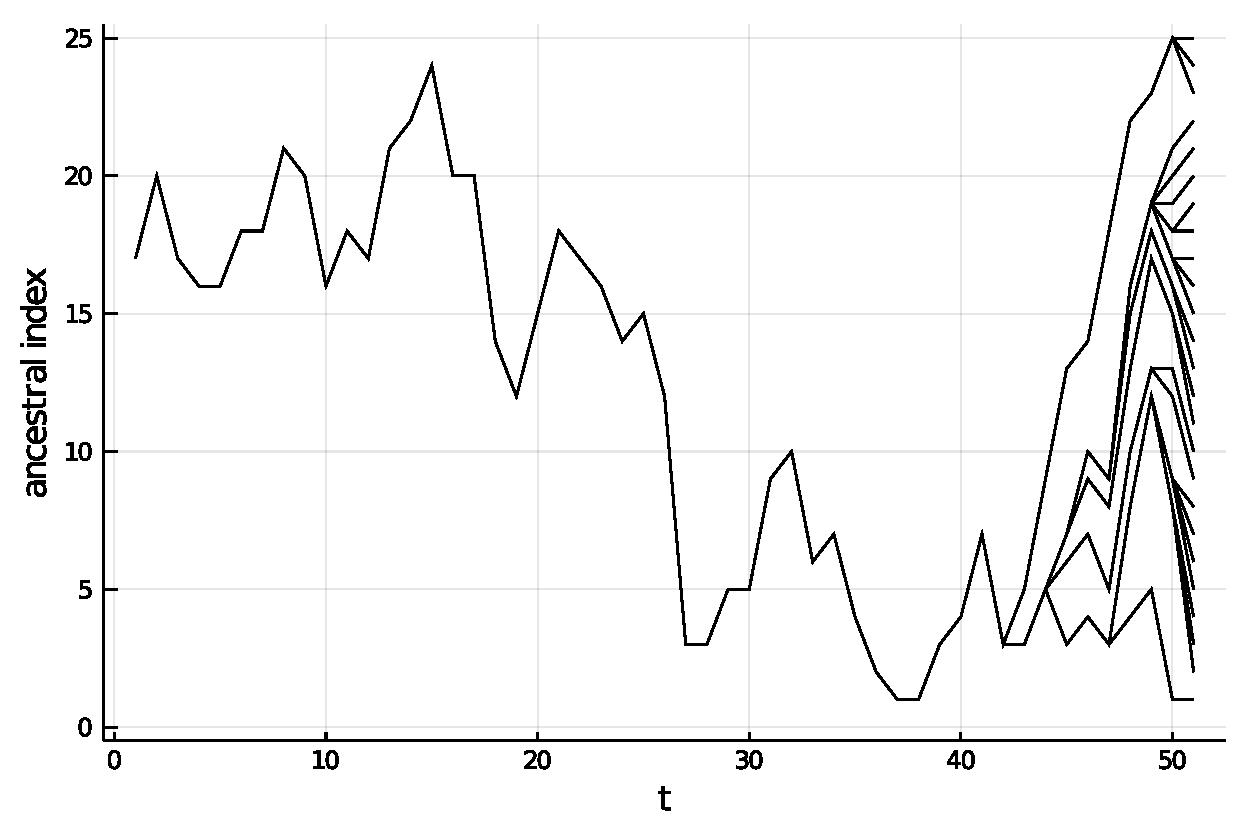
\includegraphics[width=0.47\textwidth]{../plots/ancdegen_mn.pdf}
\label{fig:ancdegen_mn}
}
\subfloat[Adaptive minimum-variance resampling]{
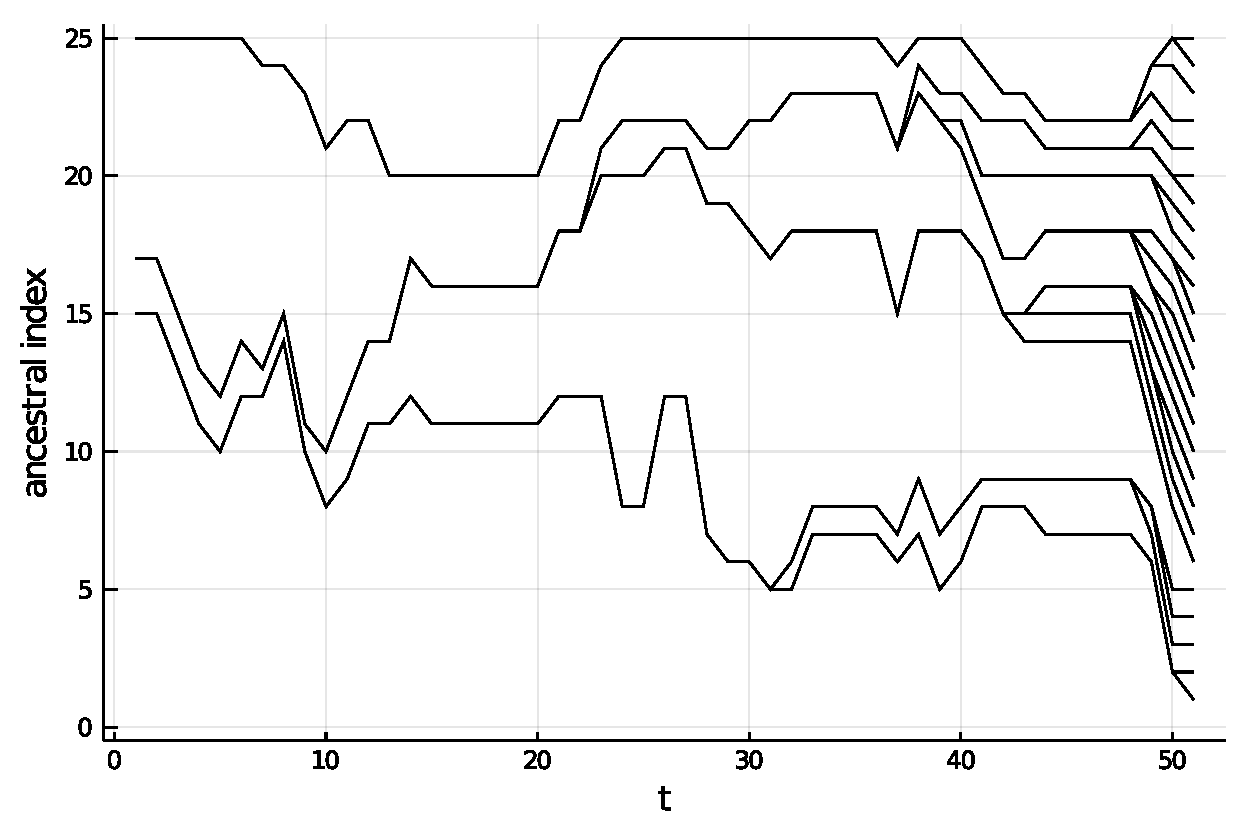
\includegraphics[width=0.47\textwidth]{../plots/ancdegen_adaptsyst.pdf}
\label{fig:ancdegen_adaptsyst}
}
\caption[Ancestral degeneracy]{Illustration of ancestral degeneracy and the mitigating effect of low-variance and adpative resampling.
Each line is the lineage of one of the terminal particles, indicating the index of its ancestor in each generation:
\subref{fig:ancdegen_mn} with multinomial resampling;
\subref{fig:ancdegen_adaptsyst} the same system with adaptive systematic resampling.}
\label{fig:ancestral_degeneracy}
\end{figure}
On the other hand, ancestral degeneracy actually improves the memory efficiency of SMC. We do not need to store all of the particles generated at each time (at memory cost $O(NT)$), only those that are included in the resulting genealogy. \textcite{jacob2015} provide an algorithm for efficient storage of the genealogy, reducing the asymptotic memory cost to $O(N\log N+T)$.
However, it is certainly still worth trying to reduce ancestral degeneracy because to achieve a given level of error with a highly degenerate system will require such a large $N$ that any such memory gains are cancelled out.
%(a) because computation is often the limiting factor rather than memory, and (b) 


\subsubsection{Mitigating ancestral degeneracy}
There are a few possible approaches to mitigating ancestral degeneracy.
Firstly, we could try to limit the number of offspring assigned to any one parent during each resampling step. We can only go so far, because we need the resampling procedure to remain unbiased (as discussed in Section~\ref{sec:SMC_FK}), but we can try to reduce the variance inherent in the resampling procedure. This idea, known as \emph{low-variance resampling}\seb{[citation?]} is explored in detail in Section~\ref{sec:resampling}.

Another idea is to resample less often. Recall that the reason for resampling is to prevent weight degeneracy (that is, one of the weights tending to one while the others tend to zero). Now we see that, while solving one type of degeneracy, resampling creates another. The effect of ancestral degeneracy is essentially the same as that of weight degeneracy: both drastically increase the variance of the resulting SMC estimators. 
We can therefore consider a trade-off between the two, which is the idea behind \emph{adaptive resampling} \parencite[Section 4]{liu1995}.
The trick is to apply the resampling step only at iterations in which a certain criterion is met. The most commonly-used criterion, suggested by \textcite[Equation (14)]{liu1995}, is based on the estimated \emph{effective sample size}
\begin{equation*}
ESS(t) := \left\{ \sum_{i=1}^N (w_t^{(i)})^2 \right\}^{-1} ,
\end{equation*}
which decreases as the weights degenerate.
The resampling step is then applied only at iterations $t$ such that $ESS(t)$ is less than some pre-specified threshold, typically $N/2$\seb{[citation?]}.

If adaptive resampling is used, some trivial changes are required to the calculation of the weights in Algorithm~\ref{alg:SMC}, to allow for the importance weights to accumulate sequentially until the particles are resampled. See e.g.\ \textcite[Section 10.2]{chopin2020} for details.

As well as mitigating ancestral degeneracy, adaptive resampling has the virtue of saving some computation (although the overall asymptotic complexity of the SMC algorithm does not change).
How effective adaptive resampling will be depends on the particular application and choice of SMC algorithm. If the proposals (i.e.\ transition kernels) are not very close to their targets then the weights will degenerate rapidly and the effective sample size criterion (or similar) will not reduce the frequency of resampling very much.

Low-variance resampling is also less effective under poor proposals: the resulting high-variance weights lead to high-variance offspring counts, even under minimum-variance resmapling schemes, because the resampling is required to be unbiased.

Adaptive resampling and low-variance resampling can be combined, and this is widely considered to be the best practice when implementing SMC.
Figure~\ref{fig:ancestral_degeneracy} compares ancestral degeneration under multinomial resampling (a relatively high variance scheme) to the same under adaptive resampling with a minimum-variance resampling scheme.
It is clear that the degeneration is much more severe in the former case.

There is one technique that completely solves the problem of ancestral degeneracy, namely \emph{backward simulation}\seb{[citation]}. This involves running an SMC algorithm as usual (the ``forward pass''), and then sampling new ancestors for each particle during an additional ``backward pass''. 
The backward-simulated parents in each generation are chosen among all $N$ particles, making use of particles that were not included in the forward-sampled trajectories.
The effect on genealogies is striking: the lineages are now sampled independently, so the coalescences caused by resampling do not feature at all in the output genealogies.

Since this work concerns genealogies induced by resampling, we will not say much more about backward simulation. There are many situations in which it is impossible to implement and therefore the study of SMC genealogies is still of interest. 
Firstly, backward simulation inherently requires a forward and backward pass through all of the data, so it cannot be implemented on-line. 
Secondly, calculating the backward-simulation probabilities requires the Markov kernels $M_t$ of the corresponding Feynman-Kac model to admit densities that can be evaluated pointwise. This is much stronger than the ability to simulate from $M_t$, the requirement for applying standard SMC algorithms.




\subsection{Asymptotic genealogies}
If we had access to information about the behaviour of SMC genealogies a priori (i.e.\ without having run the algorithm), we would be in a position to answer many questions of interest. These include practical questions about tuning, for example:
\begin{itemize}
\item How many particles should I use in order to maintain (with high enough probability) a given level of error over a time horizon $T$?
\item With $N$ particles, what is the largest lag over which fixed-lag smoothing produces reasonable estimates?
\item How many particles should I use within particle Gibbs to ensure that (with high enough probability) at least two distinct trajectories survive each iteration?
\end{itemize}
This last question touches on a critical aspect of the performance of particle Gibbs algorithms, which is discussed in Section~\ref{sec:condSMC}.
We could also consider theoretical questions, such as:
\begin{itemize}
\item For a given class of models and algorithms, what is the effect of ancestral degeneracy on how the estimators behave over time?
\item Which resampling schemes lead to the smallest amount of ancestral degeneracy?
\item What is the effect on genealogies of adaptive resampling?
\end{itemize}
Many of these questions have already been partially addressed, without any explicit analysis of genealogies, by way of variance calculations and simulation experiments.
But since these are all genealogical questions by nature, it seems sensible to work directly with the genealogies, if possible.
The problem is that the genealogy of particles is a complex object, it is random, and it can depend strongly on the particular choice of Feynman-Kac model and SMC implementation.

It turns out that these problems can be somewhat overcome by considering the genealogies in an asymptotic regime where the number of particles $N$ tends to infinity.
In this regime, many different particle systems exhibit genealogies of a common form, namely Kingman's $n$-coalescent under suitable time-scalings. The genealogical differences between various algorithms is then encoded by their respective time-scale functions. This is still a random object but is less complicated than the genealogy itself; namely a c\`adl\`ag function as opposed to a labelled weighted tree.

In the context of SMC, these asymptotic genealogies were first analysed by \textcite{koskela2018}. The simulations therein suggest that such asymptotic results also transfer to finite systems, making them practically useful.
One of the contributions of the current work is to demonstrate that Kingman-type genealogies arise from a wide variety of SMC algorithms, including those most commonly used in practice.
In principle this means, for instance, that genealogies of different SMC algorithms can be compared by examining the corresponding time-scale functions.





\section{Resampling}
\label{sec:resampling}
As we have seen, resampling is necessary within SMC to ``reset'' the weights in order to prevent weight degeneracy.
Resampling is itself a Monte Carlo procedure: the discrete offspring counts can be viewed as stochastic estimates of the continuous weights.
In order to obtain a valid SMC algorithm, these Monte Carlo samples must be unbiased; this and other desirable properties are formalised in Definition~\ref{defn:resampling}.
There is a huge range of resampling procedures satisfying these properties, some of which perform better than others. 
Some of the most popular resampling schemes are introduced in Section~\ref{sec:examples_resamplingschemes} and their properties are explored in Section~\ref{sec:resampling_properties}.




\subsection{Definition}

\begin{defn}\label{defn:resampling}
For our purposes, a valid resampling scheme is a stochastic function mapping weights 
$w_t^{(1:N)} \in \mathcal{S}_{N-1}$ 
to offspring counts 
$\nu_t^{(1:N)} \in \{0,\dots,N\}^N $
that satisfies the following properties:
\begin{enumerate}
\item\label{item:resampling_property1} the population size is conserved:
$ \sum_{i=1}^N \nu_t^{(i)} =N $
\item\label{item:resampling_property2} the weights are equal after resampling:
$w_{t+}^{(i)} = 1/N$ for all $i$
\item\label{item:resampling_property3} the resampling is unbiased:
$ \E[ \nu_t^{(i)} \mid w_t^{(i)} ] = N w_t^{(i)} $ for all $i$.
\end{enumerate}
\end{defn}
It is possible to design resampling schemes that violate these properties.
For example, a scheme of \textcite{liu1998} uses the square roots of the weights for resampling, then corrects by setting unequal weights after resampling (violating conditions \ref{item:resampling_property2} and \ref{item:resampling_property3}).
\textcite[Section 3.1]{liu2001} generalises this further, and suggests setting the resampling weights adaptively as a function of the true weights $w_t^{(1:N)}$.
\textcite{fearnhead2003} also allows the weights to be unequal after resampling; see point (d) on p.890 therein.
%
Resampling different (possibly random) numbers of particles in different iterations (violating condition \ref{item:resampling_property1}) is of course possible \parencite[see for example][]{crisan1998}, but we typically have a fixed limit on computational resources, so in most cases it makes sense to simulate the maximum feasible number of particles $N$ at every iteration.
There may be circumstances under which it is beneficial to allow the number of particles to vary adaptively or at random, but this is not commonly done in practice.
%
Deterministic resampling schemes (which cannot generally be unbiased, violating condition \ref{item:resampling_property3}) have been used by some authors. These include schemes based on optimal transport \parencite{reich2013, myers2021, corenflos2021} and the importance support points resampling of \textcite{huang2020}.
However, the majority of resampling schemes in the literature fit within Definition~\ref{defn:resampling}, and it is not typically advantageous to violate the properties \ref{item:resampling_property1}--\ref{item:resampling_property3}.

Within Definition~\ref{defn:resampling} there is still a great deal of flexibility. Many different resampling schemes have been proposed in the literature, some of which perform better than others.
 Section~\ref{sec:examples_resamplingschemes} introduces some important resampling schemes. Their properties are discussed in Section~\ref{sec:resampling_properties} and summarised in Table~\ref{tab:resampling_properties}.



\subsection{Examples}
\label{sec:examples_resamplingschemes}
\seb{Argue in each case that the scheme is unbiased?}


 
\subsubsection{Multinomial resampling}
%\label{sec:resampling_multinomial}
%\draft{Remark that this is similar to Wright-Fisher model (Section~\ref{sec:popgenmodels}), but with random non-uniform weights that are dependent over time...?}\\
Multinomial resampling \parencite{gordon1993,efron1994} is one of the simplest resampling schemes.
The parental indices are chosen independently from $\{1, \dots, N\}$, each with probability given by the weight of the corresponding particle $w_t^{(i)}$. 
That is, 
\begin{equation*}
a_t^{(1:N)} \simiid \Cat( \{1,\dots, N\}, w_t^{(1:N)} ) .
\end{equation*}
This implies that the joint distribution of the offspring counts is 
\begin{equation*}
\nu_t^{(1:N)} \eqdist \operatorname{Multinomial}(N, w_t^{(1:N)} ) .
\end{equation*}
It follows from properties of the Multinomial distribution that this resampling scheme is unbiased.
%\seb{Although the parental indices are chosen independently, the resulting offspring counts are negatively correlated. --- link to GCW19's negative association?}

A simple way to sample the parental indices is to use inversion sampling: partition the unit interval into $N$ subintervals each of which will correspond to a certain index $i$ and has length equal to the weight $w_t^{(i)}$; then draw $N$ samples $U_i \sim \Unif[0,1]$ and classify them according to which of these subintervals they fall in.
Explicitly, the parental index assigned to child $i$ is the index $a_i$ satisfying
\begin{equation}\label{eq:syst_strat_resampling}
\sum_{j=1}^{a_i -1} w_t^{(j)} \leq U_i \leq \sum_{j=1}^{a_i} w_t^{(j)} .
\end{equation}
This is illustrated in Figure \ref{fig:inv_resampling}. 
%Note that there exist more efficient methods to sample from a Multinomial distribution, so the inversion method may not be used in practice.

Fast implementations of multinomial resampling rely on $U_1,\dots,U_N$ being pre-sorted, which speeds up the search step \eqref{eq:syst_strat_resampling}. Sorting $N$ numbers requires $O(N\log N)$ computation, but this is not necessary since we can sample directly the order statistics of a $\Unif[0,1]$ distribution, at $O(N)$ cost.
One way to do this \parencite[Proposition 9.1]{chopin2020} is to sample $X_i \sim \Exp(1)$ independently for $i=1,\dots,N+1$ and output the normalised sums
\begin{equation*}
U_k := \frac{\sum_{i=1}^k X_i}{\sum_{i=1}^{N+1} X_i}
\end{equation*}
for $k=1,\dots,N$.
Another method \parencite{hol2006} is to sample $X_i \sim \Unif[0,1]$ for $i=1,\dots,N$ and compute recursively
\begin{equation*}
U_N := X_N^{1/N} , \qquad U_k := X_k^{1/k} U_{k+1} .
\end{equation*}
\seb{Does this really gives the correct distribution?}\\
This allows multinomial resampling to be implemented at $O(N)$ cost. 
A side-effect is that the sampled ancestral indices will be ordered and therefore cannot be Categorically distributed, although the offspring counts still have the correct Multinomial distribution. For the purposes of resampling this isn't usually a problem, but the Categorical distribution can anyway be restored at $O(N)$ cost by applying a random permutation to the offspring indices.




\subsubsection{Residual resampling}
%\label{sec:resampling_residual}
Residual resampling is described in \textcite{liu1998} and also in \textcite{whitley1994} where it is called ``remainder stochastic sampling''.

Each particle $X_{t}^{(i)}$ is deterministically assigned $\flnw$ offspring, and the remaining
\begin{equation*}
R := \sum_{i=1}^N ( Nw_t^{(i)} - \flnw) = N- \sum_{i=1}^N \flnw
\end{equation*}
offspring are assigned stochastically according to the residual weights
\begin{equation*}
r^{(i)} := ( Nw_t^{(i)} - \flnw) /R .
\end{equation*}
Notice that each $r^{(i)}$ lies in the interval $[0, 1/R)$, and $R\in\{0,\dots,N-1\}$ with $R=0$ only if all weights are multiples of $1/N$ in which case all residual weights are zero.

The stochastic part can be implemented using any of the other basic resampling schemes (e.g.\ multinomial, stratified, systematic). Most presentations focus on the case where multinomial resampling is used for the residuals, which is by no means the most sensible choice. We will explore several different options in what follows.

%This yields a vector of offspring counts
%\begin{equation*}
%\nu_t^{(1:N)} \eqdist \lfloor N w_t^{(1:N)} \rfloor +  \operatorname{Multinomial}(R, (N w_t^{(1:N)} - \lfloor N w_t^{(1:N)}\rfloor)/R) .
%\end{equation*}
%The deterministic part ensures that every particle with weight $>1/N$ is guaranteed to survive. This is a desirable property as it prevents the random loss of high-weighted particles.

\begin{figure}
\centering
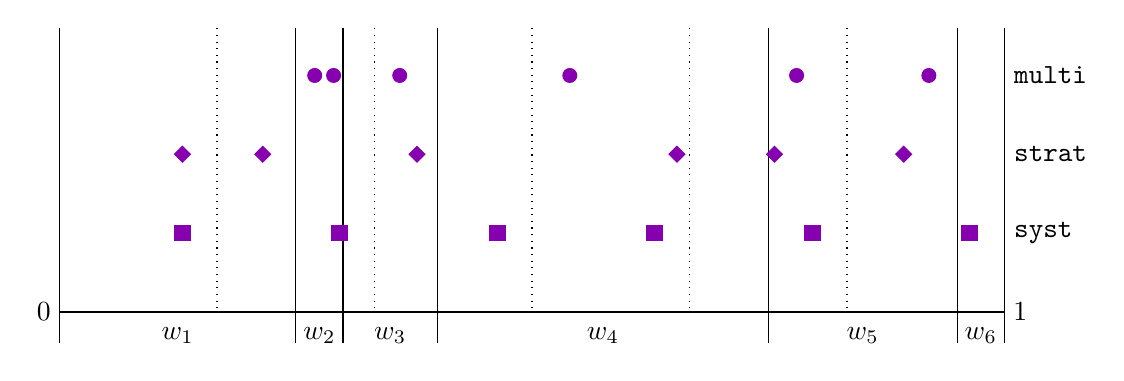
\begin{tikzpicture}
%% w = (0.25, 0.05, 0.10, 0.35, 0.20, 0.05)
%% u = (0.78, 0.29, 0.27, 0.92, 0.54, 0.36)
%%parallel lines
\draw[thick] (0,1) -- (12,1);
%\draw (0,2) -- (12,2);
%\draw (0,3) -- (12,3);
%\draw (0,4) -- (12,4);
%% endpoint labels
\node at (-0.2,1) {$0$};
\node at (12.2,1) {$1$};
%% vertical lines indicating weight intervals
\draw (0,4.6) --(0,0.6);
\draw (3,4.6) --(3,0.6);
\draw (3.6,4.6) --(3.6,0.6);
\draw (4.8,4.6) --(4.8,0.6);
\draw (9,4.6) --(9,0.6);
\draw (11.4,4.6) --(11.4,0.6);
\draw (12,4.6) --(12,0.6);
%% weight labels
\node at (1.5,0.7) {$w_1$};
\node at (3.3,0.7) {$w_2$};
\node at (4.2,0.7) {$w_3$};
\node at (6.9,0.7) {$w_4$};
\node at (10.2,0.7) {$w_5$};
\node at (11.7,0.7) {$w_6$};
%% vertical lines spaced 1/N apart
\draw[dotted] (2,4.6) --(2,1);
\draw[dotted] (4,4.6) --(4,1);
\draw[dotted] (6,4.6) --(6,1);
\draw[dotted] (8,4.6) --(8,1);
\draw[dotted] (10,4.6) --(10,1);
%% resampling scheme labels
\node[anchor=west] at (12,4) {\texttt{multi}};
\node[anchor=west] at (12,3) {\texttt{strat}};
\node[anchor=west] at (12,2) {\texttt{syst}};
%% multinomial points (top row)
\filldraw[violet] (9.36,4) circle (2.5pt);
%\node[anchor=south, violet] at (9.36,4) {$u_1$};
\filldraw[violet] (3.48,4) circle (2.5pt);
%\node[anchor=south, violet] at (3.54,4) {$u_2$};
\filldraw[violet] (3.24,4) circle (2.5pt);
%\node[anchor=south, violet] at (3.18,4) {$u_3$};
\filldraw[violet] (11.04,4) circle (2.5pt);
%\node[anchor=south, violet] at (11.04,4) {$u_4$};
\filldraw[violet] (6.48,4) circle (2.5pt);
%\node[anchor=south, violet] at (6.48,4) {$u_5$};
\filldraw[violet] (4.32,4) circle (2.5pt);
%\node[anchor=south, violet] at (4.32,4) {$u_6$};
%% stratified points (middle row)
\filldraw[violet] (1.46,3)--(1.56,3.1)--(1.66,3)--(1.56,2.9)--cycle;
%\node[anchor=south, violet] at (1.56,3) {$u_1$};
\filldraw[violet] (2.48,3)--(2.58,3.1)--(2.68,3)--(2.58,2.9)--cycle;
%\node[anchor=south, violet] at (2.58,3) {$u_2$};
\filldraw[violet] (4.44,3)--(4.54,3.1)--(4.64,3)--(4.54,2.9)--cycle;
%\node[anchor=south, violet] at (4.54,3) {$u_3$};
\filldraw[violet] (7.74,3)--(7.84,3.1)--(7.94,3)--(7.84,2.9)--cycle;
%\node[anchor=south, violet] at (7.84,3) {$u_4$};
\filldraw[violet] (8.98,3)--(9.08,3.1)--(9.18,3)--(9.08,2.9)--cycle;
%\node[anchor=south, violet] at (9.12,3) {$u_5$};
\filldraw[violet] (10.62,3)--(10.72,3.1)--(10.82,3)--(10.72,2.9)--cycle;
%\node[anchor=south, violet] at (10.72,3) {$u_6$};
%% systematic points (bottom row)
\filldraw[violet] (1.46,1.9)--(1.46,2.1)--(1.66,2.1)--(1.66,1.9)--cycle;
%\node[anchor=south, violet] at (1.56,2) {$u_1$};
\filldraw[violet] (3.46,1.9)--(3.46,2.1)--(3.66,2.1)--(3.66,1.9)--cycle;
%\node[anchor=south, violet] at (3.56,2) {$u_2$};
\filldraw[violet] (5.46,1.9)--(5.46,2.1)--(5.66,2.1)--(5.66,1.9)--cycle;
%\node[anchor=south, violet] at (5.56,2) {$u_3$};
\filldraw[violet] (7.46,1.9)--(7.46,2.1)--(7.66,2.1)--(7.66,1.9)--cycle;
%\node[anchor=south, violet] at (7.56,2) {$u_4$};
\filldraw[violet] (9.46,1.9)--(9.46,2.1)--(9.66,2.1)--(9.66,1.9)--cycle;
%\node[anchor=south, violet] at (9.56,2) {$u_5$};
\filldraw[violet] (11.46,1.9)--(11.46,2.1)--(11.66,2.1)--(11.66,1.9)--cycle;
%\node[anchor=south, violet] at (11.56,2) {$u_6$};
\end{tikzpicture}
\caption[Inversion sampling for multinomial, stratified and systematic resampling]{Inversion sampling interpretation of multinomial, stratified and systematic resampling.
In this example, $N=6$, $w^{(1:6)} = (0.25,0.05,0.1,0.35,0.2,0.05)$ and the uniform random variables input to the resampling schemes are $u_{1:6} = (0.78, 0.29, 0.27, 0.92, 0.54, 0.36)$.
The solid vertical lines show the partition of $[0,1]$ into subintervals with lengths $w^{(1:6)}$.
The dotted vertical lines show the partition of $[0,1]$ into subintervals of length $1/N$, used for stratified and systematic resampling.\\
Top row (circles): in multinomial resampling, $u_{1:6}$ are fed directly into the inversion sampler. Which subinterval $u_i$ falls into determines the parent of offspring $i$. The resulting offspring counts in this example are $\nu^{(1:6)} = (0,2,1,1,2,0)$.\\
Middle row (diamonds): in stratified resampling, $u_{1:6}$ are transformed so that one point lies in each subinterval of length $1/N$. The resulting offspring counts are $\nu^{(1:6)} = (2,0,1,1,2,0)$.\\
Bottom row (squares): in systematic resampling, only $u_1$ is used, being transformed to equally spaced points. The resulting offspring counts are $\nu^{(1:6)} = (1,1,0,2,1,1)$.}
\label{fig:inv_resampling}
\end{figure}
%\begin{figure}
%\centering
%\subfloat[Multinomial resampling]{
%\begin{tikzpicture}
%%parallel lines
%\draw[thick] (0,0) -- (12,0);
%\draw (0,2) -- (12,2);
%% tick marks at ends
%\draw[thick] (0,0.1) --(0,-0.1);
%\draw[thick] (12,0.1) --(12,-0.1);
%\draw (0,2.1) --(0,1.9);
%\draw (12,2.1) --(12,1.9);
%% tick marks indicating weights
%\draw[thick] (3,0.1) --(3,-0.1);
%\draw[thick] (5,0.1) --(5,-0.1);
%\draw[thick] (11,0.1) --(11,-0.1);
%% weight labels
%\node at (1.5,-0.3) {$w_1$};
%\node at (4,-0.3) {$w_2$};
%\node at (8,-0.3) {$w_3$};
%\node at (11.5,-0.3) {$w_4$};
%% endpoint labels
%\node at (-0.2,2) {$0$};
%\node at (12.2,2) {$1$};
%% uniform points
%\filldraw[violet] (10.94,2) circle (2pt);
%\filldraw[violet] (1.06,2) circle (2pt);
%\filldraw[violet] (8.82,2) circle (2pt);
%\filldraw[violet] (3.16,2) circle (2pt);
%% arrows from random points
%\draw[thick, violet, ->] (10.94,2) -- (10.94,0);
%\draw[thick, violet, ->] (1.06,2) -- (1.06,0);
%\draw[thick, violet, ->] (8.82,2) -- (8.82,0);
%\draw[thick, violet, ->] (3.16,2) -- (3.16,0);
%\end{tikzpicture}
%\label{fig:resampling_mn}
%}\\
%\subfloat[Stratified resampling]{
%\begin{tikzpicture}
%%parallel lines
%\draw[thick] (0,0) -- (12,0);
%\draw (0,2) -- (12,2);
%% tick marks at ends
%\draw[thick] (0,0.1) --(0,-0.1);
%\draw[thick] (12,0.1) --(12,-0.1);
%\draw (0,2.1) --(0,1.9);
%\draw (12,2.1) --(12,1.9);
%% tick marks indicating weights
%\draw[thick] (3,0.1) --(3,-0.1);
%\draw[thick] (5,0.1) --(5,-0.1);
%\draw[thick] (11,0.1) --(11,-0.1);
%% tick marks indicating sampling intervals:
%\draw (3,2.1) --(3,1.9);
%\draw (6,2.1) --(6,1.9);
%\draw (9,2.1) --(9,1.9);
%% weight labels
%\node at (1.5,-0.3) {$w_1$};
%\node at (4,-0.3) {$w_2$};
%\node at (8,-0.3) {$w_3$};
%\node at (11.5,-0.3) {$w_4$};
%% endpoint labels
%\node at (-0.2,2) {$0$};
%\node at (12.2,2) {$1$};
%% stratified points
%\filldraw[violet] (2.735,2) circle (2pt);
%\filldraw[violet] (3.265,2) circle (2pt);
%\filldraw[violet] (8.205,2) circle (2pt);
%\filldraw[violet] (9.79,2) circle (2pt);
%% arrows from random points
%\draw[thick, violet, ->] (2.735,2) -- (2.735,0);
%\draw[thick, violet, ->] (3.265,2) -- (3.265,0);
%\draw[thick, violet, ->] (8.205,2) -- (8.205,0);
%\draw[thick, violet, ->] (9.79,2) -- (9.79,0);
%\end{tikzpicture}
%\label{fig:resampling_stratified}
%}\\
%\subfloat[Systematic resampling]{
%\begin{tikzpicture}
%%parallel lines
%\draw[thick] (0,0) -- (12,0);
%\draw (0,2) -- (12,2);
%% tick marks at ends
%\draw[thick] (0,0.1) --(0,-0.1);
%\draw[thick] (12,0.1) --(12,-0.1);
%\draw (0,2.1) --(0,1.9);
%\draw (12,2.1) --(12,1.9);
%% tick marks indicating weights
%\draw[thick] (3,0.1) --(3,-0.1);
%\draw[thick] (5,0.1) --(5,-0.1);
%\draw[thick] (11,0.1) --(11,-0.1);
%% tick marks indicating sampling intervals:
%\draw (3,2.1) --(3,1.9);
%\draw (6,2.1) --(6,1.9);
%\draw (9,2.1) --(9,1.9);
%% weight labels
%\node at (1.5,-0.3) {$w_1$};
%\node at (4,-0.3) {$w_2$};
%\node at (8,-0.3) {$w_3$};
%\node at (11.5,-0.3) {$w_4$};
%% endpoint labels
%\node at (-0.2,2) {$0$};
%\node at (12.2,2) {$1$};
%% stratified points
%\filldraw[violet] (2.735,2) circle (2pt);
%\filldraw[violet] (5.735,2) circle (2pt);
%\filldraw[violet] (8.735,2) circle (2pt);
%\filldraw[violet] (11.735,2) circle (2pt);
%% arrows from random points
%\draw[thick, violet, ->] (2.735,2) -- (2.735,0);
%\draw[thick, violet, ->] (5.735,2) -- (5.735,0);
%\draw[thick, violet, ->] (8.735,2) -- (8.735,0);
%\draw[thick, violet, ->] (11.735,2) -- (11.735,0);
%\end{tikzpicture}
%\label{fig:resampling_systematic}
%}\\
%\caption[Inversion sampling for multinomial, stratified and systematic resampling]{Inversion sampling to obtain Multinomial offspring counts, where the (marginally) Uniform variables for inversion are sampled in different ways. For this example $N=4$ and the weights are $w_{(1:4)} = \frac{1}{N}(1,\frac{2}{3},2,\frac{1}{3})$. 
%%In each case the samples to be inverted are seeded with the same $\Unif(0,1)$ samples.
%%\subref{fig:resampling_mn} Sample $N$  independent $\Unif(0,1)$ random variables. In this example the sampled offspring counts are $(1,1,2,0)$.
%%\subref{fig:resampling_stratified} The $\Unif(0,1)$ samples are transformed to Uniform draws from the intervals (0,0.25), (0.25,0.5), (0.5, 0.75), (0.75,1). In this example the sampled offspring counts are $(1,1,2,0)$.
%%\subref{fig:resampling_systematic} Use only the first draw and transform it to a sample from $\Unif(0,0.25)$. For the subsequent samples, add 0.25 each time to obtain a sample in each interval. In this example the sampled offspring counts are $(1,0,2,1)$.
%}
%\end{figure}



\subsubsection{Stratified resampling}
%\label{sec:resampling_stratified}
Stratified resampling was introduced by \textcite{kitagawa1996}.
As in multinomial resampling, inversion sampling is used sample the parental indices. However, the samples used for inversion sampling are no longer i.i.d. $\Unif[0,1]$ samples. Instead, one number is sampled independently from each subinterval of length $1/N$; that is, 
\begin{equation*}
U_i \sim \Unif \left[\frac{i-1}{N}, \frac{i}{N} \right] .
\end{equation*}
Alternatively, one may think of standard Uniform samples $u_1,\dots,u_N \sim^{iid} \Unif[0,1]$ with the transformation
\begin{equation*}
U_i = \frac{u_i + i -1}{N} .
\end{equation*}
%to give the stratified samples $U_1,\dots,U_N$.

The parents are then assigned as in \eqref{eq:syst_strat_resampling}, illustrated in Figure \ref{fig:inv_resampling}.
The offspring distribution is no longer Multinomial, since parental indices are not identically distributed.
Stratified resampling ensures that the samples are ``well spread out'', which reduces the probability of randomly losing high-weight particles or duplicating low-weight particles.

It will be useful later on to have a better idea about the marginal distributions of $\nu_t^{(i)}$ that are induced by stratified resampling. There are complex dependencies between the offspring counts, but we can still find some constraints on the distribution of each count conditional on the corresponding weight.
Write the $i^{th}$ weight in the form $w_t^{(i)} = (K + \delta)/N$, where $\delta \in [0,1)$ and $K\in \{0,\dots,N\}$.
Considering the illustration Figure~\ref{fig:inv_resampling}, the distribution of $\nu_t^{(i)}$ depends not only on $w_t^{(i)}$ but also on where the $i^{th}$ weight interval falls with respect to the length-$(1/N)$ intervals. 
Denote the ``left overhang'' by $\delta_L$.
There are two cases to consider, which are illustrated in Figure~\ref{fig:strat_cases}.
In Case~\subref{fig:strat_case1} the total overhang is less than $1/N$ and $\delta_L \in [0,\delta]$.
In Case~\subref{fig:strat_case2} the total overhang is greater than $1/N$ and $\delta_L \in (\delta, 1)$.
%The distinction between Cases \subref{fig:strat_case1} and \subref{fig:strat_case2} is whether the ``overhang'' is less than or greater than $1/N$. 
Arrangements such that one or both ends have no overhang are special cases of Case \subref{fig:strat_case1} where $\delta_L \in \{0,\delta\}$.
Note that Case \subref{fig:strat_case2} cannot occur if $K=0$.

%\begin{figure}
%\centering
%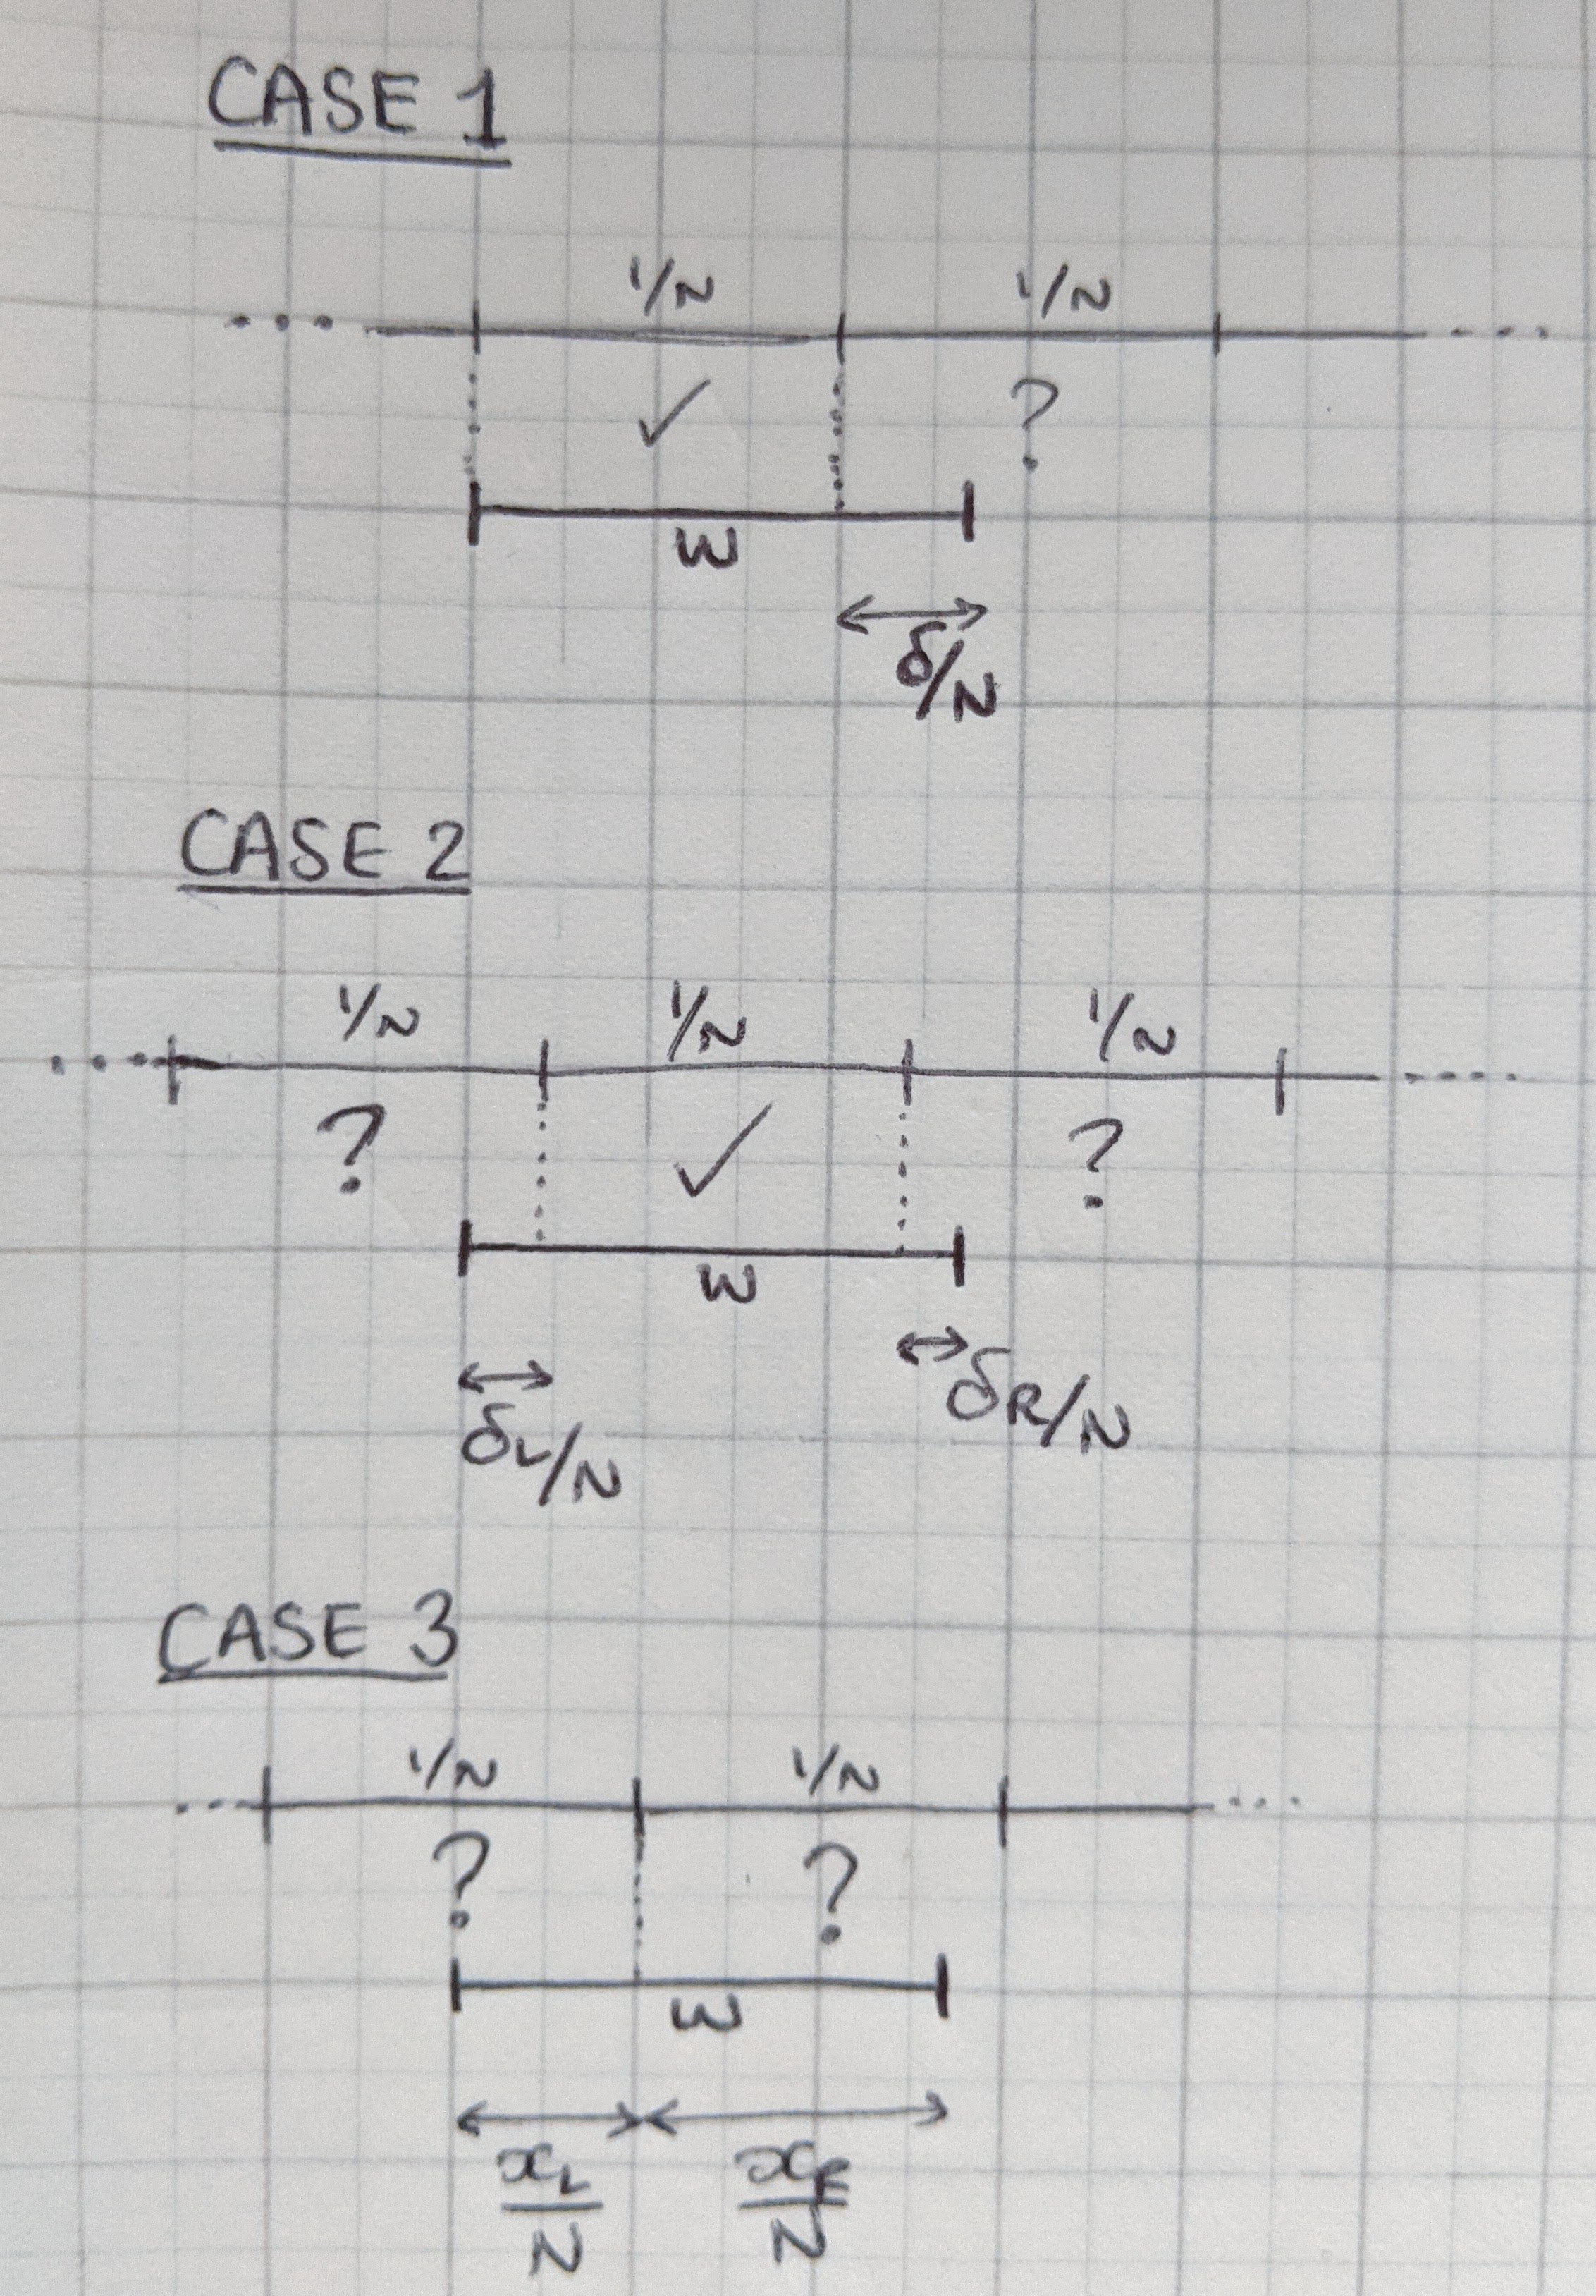
\includegraphics[width=0.4\textwidth]{plots/cases_sketch.jpg}
%\caption[PLACEHOLDER Cases for stratified resampling with a fixed weight]{PLACEHOLDER Cases for stratified resampling with a fixed weight. When I make this properly I need to allow for general $k$ rather than fixing $k=1$ as done here. Case 3 is only valid for $k\geq1$.}
%\label{fig:strat_cases_temp}
%\end{figure}

\begin{figure}
\centering
%\subfloat[Case 1]{
%\begin{tikzpicture}
%% w subinterval
%\draw[thick] (0,0)--(1.9,0);
%\draw[thick,dotted] (1.9,0)--(2.3,0);
%\draw[thick] (2.3,0)--(4.8,0);
%\draw[thick] (0,0.1)--(0,-0.1);
%\draw[thick] (4.8,0.1)--(4.8,-0.1);
%\node[anchor=north] at (2.4,0) {$w$};
%% length labels
%\draw[<->] (0,-0.4)--(4,-0.4);
%\node[anchor=north] at (2,-0.4) {$k/N$};
%\draw[<->] (4,-0.4)--(4.8,-0.4);
%\node[anchor=north] at (4.4,-0.4) {$\delta/N$};
%% sampling interval
%\draw (-0.5,1.5)--(8.5,1.5);
%\draw[dotted] (-1,1.5)--(-0.5,1.5);
%\draw[dotted] (8.5,1.5)--(9,1.5);
%\draw (0,1.6)--(0,1.4);
%\draw (4,1.6)--(4,1.4);
%\draw (8,1.6)--(8,1.4);
%\node[anchor=south] at (2,1.5) {$k/N$};
%\node[anchor=south] at (6,1.5) {$1/N$};
%% vertical dividers
%\draw[dashed, gray] (0,1.4)--(0,0.1);
%\draw[dashed, gray] (4,1.4)--(4,0.1);
%\end{tikzpicture}
%}\\
\subfloat[The overhang is less than $1/N$ and $ \delta_L \in {[0, \delta]} $. The parent under consideration is automatically assigned $K$ offspring, plus up to two more.]{
\begin{tikzpicture}
% w subinterval
\draw[thick] (0,0)--(1.9,0);
\draw[thick,dotted] (1.9,0)--(2.3,0);
\draw[thick] (2.3,0)--(4.8,0);
\draw[thick] (0,0.1)--(0,-0.1);
\draw[thick] (4.8,0.1)--(4.8,-0.1);
\node[anchor=north] at (2.4,0) {$w$};
% length labels
\draw[<->] (0.3,-0.4)--(4.3,-0.4);
\node[anchor=north] at (2,-0.4) {$\frac{K}{N}$};
\draw[<->] (4.3,-0.4)--(4.8,-0.4);
\node[anchor=north] at (4.55,-0.4) {$\frac{\delta-\delta_L}{N}$};
\draw[<->] (0,-0.4)--(0.3,-0.4);
\node[anchor=north] at (0.15,-0.4) {$\frac{\delta_L}{N}$};
% sampling interval
\draw (-4.2,1.5)--(8.8,1.5);
\draw[dotted] (-4.7,1.5)--(-4.2,1.5);
\draw[dotted] (8.8,1.5)--(9.3,1.5);
\draw (-3.7,1.6)--(-3.7,1.4);
\draw (0.3,1.6)--(0.3,1.4);
\draw (4.3,1.6)--(4.3,1.4);
\draw (8.3,1.6)--(8.3,1.4);
\node[anchor=south] at (-1.7,1.5) {$\frac{1}{N}$};
\node[anchor=south] at (2.3,1.5) {$\frac{K}{N}$};
\node[anchor=south] at (6.3,1.5) {$\frac{1}{N}$};
% vertical dividers
\draw[dashed, gray] (0.3,1.4)--(0.3,0.1);
\draw[dashed, gray] (4.3,1.4)--(4.3,0.1);
% fudge bottom space
\draw[white] (0,-1.3)--(1,-1.3);
\end{tikzpicture}
\label{fig:strat_case1}
}\\
\subfloat[The overhang is greater than $1/N$ (this case can only occur when $K\geq1$) and $\delta_L \in (\delta,1)$. The parent under consideration is automatically assigned $K-1$ offspring, plus up to two more.]{
\begin{tikzpicture}
% w subinterval
\draw[thick] (-2,0)--(1.9,0);
\draw[thick,dotted] (1.9,0)--(2.3,0);
\draw[thick] (2.3,0)--(6.8,0);
\draw[thick] (-2,0.1)--(-2,-0.1);
\draw[thick] (6.8,0.1)--(6.8,-0.1);
\node[anchor=north] at (2.4,0) {$w$};
% length labels
\draw[<->] (0.3,-0.4)--(4.3,-0.4);
\node[anchor=north] at (2,-0.4) {$\frac{K-1}{N}$};
\draw[<->] (4.3,-0.4)--(6.8,-0.4);
\node[anchor=north] at (5.55,-0.4) {$\frac{1+\delta-\delta_L}{N}$};
\draw[<->] (-2,-0.4)--(0.3,-0.4);
\node[anchor=north] at (-1.15,-0.4) {$\frac{\delta_L}{N}$};
% sampling interval
\draw (-4.2,1.5)--(8.8,1.5);
\draw[dotted] (-4.7,1.5)--(-4.2,1.5);
\draw[dotted] (8.8,1.5)--(9.3,1.5);
\draw (-3.7,1.6)--(-3.7,1.4);
\draw (0.3,1.6)--(0.3,1.4);
\draw (4.3,1.6)--(4.3,1.4);
\draw (8.3,1.6)--(8.3,1.4);
\node[anchor=south] at (-1.7,1.5) {$\frac{1}{N}$};
\node[anchor=south] at (2.3,1.5) {$\frac{K-1}{N}$};
\node[anchor=south] at (6.3,1.5) {$\frac{1}{N}$};
% vertical dividers
\draw[dashed, gray] (0.3,1.4)--(0.3,0.1);
\draw[dashed, gray] (4.3,1.4)--(4.3,0.1);
% fudge bottom space
\draw[white] (0,-1.3)--(1,-1.3);
\end{tikzpicture}
\label{fig:strat_case2}
}
\caption[Cases for stratified resampling with a fixed weight]{Cases for stratified resampling with a fixed weight $w = (K+\delta)/N$.}
\label{fig:strat_cases}
\end{figure}


In any case $\nu_t^{(i)} \in \{K-1, K, K+1, K+2\}$ almost surely. 
To define a probability distribution over these four values, we introduce the notation
\begin{equation*}
p_j := \Prob[ \nu_t^{(i)} = \flnw +j \mid w_t^{(i)} ] ,
\end{equation*}
for $j=-1,0,1,2$.
%\seb{Change notation to avoid confusion with $p_k^{(i)}$'s in Chapter~\ref{ch:appl}?}
Since the sample within each interval of length $1/N$ is uniform over that interval, we find the probabilities given in Table~\ref{tab:strat_probs}, in terms of $\delta$ and $\delta_L$. The probabilities do not depend on $K$, but of course the corresponding values of $\nu_t^{(i)}$ do.

\begin{table}[ht]
\centering
\begin{tabular}{ c | c c | c c }
\hline\hline
& Case \subref{fig:strat_case1} & Case \subref{fig:strat_case2} & L.B. & U.B. \\
\hline
$p_{-1}$ & 0 & $\delta_L(1+\delta - \delta_L) -\delta$ & 0 & $1/4$ \\
$p_0$ & $1-\delta + \delta_L(\delta -\delta_L)$ 
        & $1+\delta-2\delta_L(1+\delta -\delta_L)$ & $(1-\delta) /2$ 
        & $1 - 3\delta /4$ \\
$p_1$ & $\delta-2\delta_L(\delta -\delta_L)$ & $\delta_L(1+\delta -\delta_L)$ 
        & $\delta /2$ & $(1+\delta)/2$ \\
$p_2$ & $\delta_L(\delta -\delta_L)$ & 0 & 0 & $1/4$ \\
\hline\hline
\end{tabular}
\caption[Distribution of offspring counts under stratified resampling]{Marginal probability distribution of $\nu_t^{(i)}$ conditional on $w_t^{(i)} = (K+\delta)/N$, in terms of $\delta$ and the left overhang $\delta_L$, along with upper and lower bounds on these in terms of $\delta$ only, which hold in both cases.}
\label{tab:strat_probs}
\end{table}

%By considering the constraints on $\delta_L, \delta_R, x_L, x_R$, we also have the following properties which hold in every case (i.e.\ for any $w_t^{(i)}$):
%\begin{itemize}
%\item $p_{-1} \leq 1/4$
%\item $p_{2} \leq 1/4$
%\item only one of $p_{-1}, p_2$ can be non-zero.
%\end{itemize}





\subsubsection{Systematic resampling}
%\label{sec:resampling_systematic}
Systematic resampling is described in \textcite{carpenter1999} and also in \textcite{whitley1994} where it is called ``stochastic universal sampling''.

Like stratified resampling, it uses the inversion sampler of multinomial resampling but starts with a more regular set of points in $[0,1]$.
In this scheme, only one standard Uniform sample is drawn, $u \sim \Unif[0,1]$, from which the $N$ samples are generated by via the transformation
\begin{equation*}
U_i = \frac{u+ i-1}{N}
\end{equation*}
for $i = 1, \dots, N $.
The parental indices are again selected according to \eqref{eq:syst_strat_resampling}, as illustrated in Figure \ref{fig:inv_resampling}.

\textcite{kitagawa1996} suggests a deterministic scheme in which the random $u$ is replaced by a fixed $\alpha\in[0,1]$; but, being deterministic, this scheme does not satisfy the unbiasedness condition (Property~\ref{item:resampling_property1} in Definition~\ref{defn:resampling}).
\textcite{whitley1994} employs a different description of systematic resampling, where the interval $[0,1]$ is joined up into a circle, and the systematic samples are evenly spaced pointers on an outer ring, which is spun around like a roulette wheel. This comprises adding a random phase to each $U_i$, modulo one, and is an exactly equivalent description of systematic resampling.\seb{Diagram?}

Like stratified resampling, systematic resampling ensures the random numbers are ``well spread out''; the resulting samples are even more constrained than with stratified resampling. 
Systematic resampling also has the advantage of being extremely easy to implement and computationally efficient, requiring only one sample from a pseudo-random number generator (PRNG) followed by $O(N)$ elementary operations.

However, the systematic scheme is known to exhibit pathological behaviour in some cases because its performance depends on the ordering of the weights. A simple example of this phenomenon is presented in \textcite{douc2005}. 
Such behaviour can be avoided by randomly permuting the weights before resampling, and this is the recommended practice\seb{[citation?]}. 



\subsubsection{Star resampling}
%\label{sec:resampling_star}
For the sake of comparison, we also construct a resampling scheme which is in some sense the worst possible.
Sample
\begin{equation*}
a \sim \Cat( \{1,\dots, N\}, w_t^{(1:N)} )
\end{equation*}
and set $a_t^{(i)} = a$ for all $i$.
The resulting offspring counts are all equal to zero except for $\nu_t^{(a)}$, which is equal to $N$.
This resampling scheme is indeed unbiased, since each offspring count has marginal distribution
\begin{equation*}
\nu_t^{(i)}  \mid w_t^{(1:N)} 
= \begin{cases}
0 & \text{w.p. } 1-w_t^{(i)} \\
N & \text{w.p. } w_t^{(i)} .
\end{cases}
\end{equation*}
These offspring counts have the highest possible marginal variance subject to $\E[ \nu_t^{(i)}  \mid w_t^{(i)} ] = Nw_t^{(i)}$ and $\nu_t^{(i)} \in \{0,\dots,N\}$.

I call this scheme \emph{star resampling} because the parent-offspring relationships at each iteration form a star graph.


\subsubsection{Minimal variance branching}
The minimal variance branching (MVB) algorithm of \textcite{crisan1999} provides a framework for resampling that enforces the minimal variance. 
It requires that each offspring count $\nu_t^{(i)}$, conditionally on $w_t^{(i)}$, has marginal distribution
\begin{equation}\label{eq:branching_distn}
\nu_t^{(i)} \mid w_t^{(i)} \eqdist \flnw + \Bern(Nw_t^{(i)} - \flnw) .
\end{equation}
We will see later on that this is exactly the framework of \emph{stochastic rounding}.

The set-up of \textcite{crisan1999} does not require the number of particles to remain constant from one generation to the next (Property~\ref{item:resampling_property1} in Definition~\ref{defn:resampling}), so the MVB algorithm could be implemented for instance by sampling each $\nu_t^{(i)}$ independently from \eqref{eq:branching_distn}. The authors remark that enforcing strictly negative correlation between the offspring counts can improve the rate of convergence, but they do not specify how this might be achieved.
\seb{Could argue therefore that we'll just ignore this resampling scheme from now on, since we don't know how to make it fit Definition~\ref{defn:resampling}.}


\subsubsection{Srinivasan sampling procedure}
\textcite{gerber2017} build on the work of \textcite{crisan1999} in that they construct a resampling scheme for which the marginal offspring counts are distributed as \eqref{eq:branching_distn}, but the number of particles is held constant and non-negative correlation of offspring counts is enforced. The resulting scheme is termed \emph{Srinivasan sampling procedure (SSP) resampling} after \textcite{srinivasan2001}.

The implementation is somewhat complicated compared to the other schemes we have seen \parencite[for full details see][Algorithm~1]{gerber2017} but a brief description is given here.
The offspring counts are initialised at $Nw_t^{(i)}$, then we iterate through pairs of counts, rounding one of the pair up and the other down by an amount such that at least one of the pair ends up an integer. After at most $N$ such adjustments, all of the counts are integers and can be returned. Each iteration adds and subtracts the same amount so that the sum of the counts is preserved, ensuring that the number of particles remains constant. Which of the selected pair is increased/decreased in each iteration is chosen at random with probabilities that guarantee the resampling is unbiased.

As well as proposing this resampling scheme, \textcite{gerber2017} make several other contributions to the SMC resampling literature, some of which will be discussed later.


\begin{table}[ht]
\centering
\begin{tabular}{ l l }
\hline\hline
Abbreviation & Description \\% & Defined in Section \\
\hline
\texttt{multi} & multinomial resampling \\%& \ref{sec:resampling_multinomial} \\
\texttt{star} & star resampling \\%& \ref{sec:resampling_star} \\
\texttt{strat} & stratified resampling \\%& \ref{sec:resampling_stratified} \\
\texttt{syst} & systematic resampling \\%& \ref{sec:resampling_systematic} \\
\texttt{res-multi} & residual resampling with multinomial residuals \\
        %& \ref{sec:resampling_residual} \\
\texttt{res-star} & residual resampling with star residuals \\
        %& \ref{sec:resampling_residual} \\
\texttt{res-strat} & residual resampling with stratified residuals \\
        %& \ref{sec:resampling_residual} \\
\texttt{res-syst} & residual resampling with systematic residuals \\
        %& \ref{sec:resampling_residual} \\
\texttt{ssp} & Srinivasan sampling procedure resampling \\%& \\
\texttt{mvb} & minimal variance branching algorithm \\%& \\
\hline\hline
\end{tabular}
\caption{Abbreviations for resampling schemes}
\label{tab:resampling_abbrevs}
\end{table} 





\subsection{Properties}\label{sec:resampling_properties}
In this section we consider some important properties of resampling schemes, and see how the example schemes of Section~\ref{sec:examples_resamplingschemes} compare in terms of these.
The findings are summarised in Table~\ref{tab:resampling_properties}, with the exception of a few properties which depend on details of the implementation or are applicable only to a subset of the resampling schemes considered.


\subsubsection{Support of offspring numbers}
Recall that the weights give an indication of how ``useful'' each particle is for the approximation. Killing a high-weight particle is likely to increase the variance of the SMC estimates, while duplicating a low-weight particle wastes computational resources on propagating particles that will not contribute much to reducing that variance.
One way to assess the performance of a given resampling scheme, then, is to consider the support of the marginal offspring distributions, conditional on the weights. This tells us how many duplicates it is possible to obtain from a particle with a given weight, and is therefore an indication of performance, albeit a rather crude one.

Suppose that $w_t^{(i)} \in [K/N, (K+1)/N]$. The value of $K$ roughly determines how useful particle $i$ is. Conditional on $K$, we will determine the range of possible values $\nu_t^{(i)}$ can take, under each  of the resampling schemes described in Section~\ref{sec:examples_resamplingschemes}.

Under multinomial resampling, it is possible for $\nu_t^{(i)}$ to take any value from $0$ to $N$ (although some values are of course more likely than others).
Thus it is possible for a high-weight particle to have zero offspring, or a low-weight particle to have many offspring, simply by chance.

Residual resampling ensures that every particle with above-average (i.e.\ $>1/N$) weight has at least one offspring, avoiding the loss of high-weight particles. If the residuals are sampled using multinomial resampling then the duplication of low-weight particles is not avoided, $\nu_t^{(i)} \in \{K, \dots, K+R\} \subseteq \{K,\dots, N\}$, but this can be addressed by using a lower-variance scheme for the residual offspring. Various choices are included in Table~\ref{tab:resampling_properties}.

Stratified resampling is more restrictive, $\nu_t^{(i)} \in \{ K-1, K, K+1, K+2 \}$, but allows the possibility of a particle with above-average weight having no offspring. This is not quite as good as the erroneous claim of \textcite{douc2005} that $| \nu_t^{(i)} - Nw_t^{(i)} | \leq 1$ for stratified resampling.
Systematic resampling has the smallest support, $\nu_t^{(i)} \in \{K, K+1\}$, that is possible whilst maintaining unbiasedness, as do SSP and MVB resampling.

Another way to quantify this property is by considering the maximum possible difference between the offspring count $\nu_t^{(i)}$ and its expected value $N w_t^{(i)}$. This is also presented in Table~\ref{tab:resampling_properties}.




\subsubsection{Degeneracy under equal weights}
In the case where all of the weights are multiples of $1/N$, low-variance schemes such as residual and systematic resampling become fully deterministic. 
Since $\flnw = Nw_t^{(i)}$ for each $i$, residual resampling will have $R=0$, leaving no remainder to be assigned stochastically. 
In systematic resampling exactly $\flnw = Nw_t^{(i)}$ samples will fall in the $i^{th}$ interval.
In particular, if $w_t^{(1:N)} = (1,\dots, 1)/N$ then each parent is assigned exactly one offspring deterministcially, so there is effectively no resampling.

The same phenomenon occurs with stratified resampling, although not if one uses Whitley's roulette wheel description\seb{(Figure ??)}. The random phase shift introduced by ``spinning the wheel'' prevents the inversion sampling intervals from lining up exactly with the weight intervals, so the resampled offspring counts may vary from their means by one either side.
\textcite{whitley1994} does not describe stratified resampling, but we see that unlike with systematic resampling, in the case of startified resampling the roulette wheel description is not equivalent to the standard inversion sampling description. 
The roulette wheel adds some unnecessary extra randomness, so the straightforward inversion sampler is preferred.

If the state space is continuous, the event that all weights are multiples of $1/N$ typically has zero measure, but with non-zero probability we can get arbitrarily close to this regime in which resampling becomes deterministic.




\subsubsection{Marginal variance of offspring counts}
%\draft{Mention negative association? $=$ teaser for later, which has to do with covariance between counts rather than marginal variance.}
Another indication of the performance of resampling is the variance of the resampled offspring counts. For instance we might ask what is the marginal variance of $\nu_t^{(i)}$, conditional on the corresponding weight $w_t^{(i)}$. We would like to keep this variance small, limiting the additional randomness introduced to our Monte Carlo estimates by the resampling step.

In multinomial resampling, the marginal distributions are
\begin{equation*}
\nu_t^{(i)} \mid w_t^{(i)} 
\eqdist \Bin(N, w_t^{(i)})
\end{equation*}
so the variance is
\begin{equation*}
\V[ \nu_t^{(i)} \mid w_t^{(i)} ]
= N w_t^{(i)} ( 1- w_t^{(i)} ) .
\end{equation*}
Compare this to star resampling, where the marginal offspring counts
\begin{equation*}
\nu_t^{(i)} \mid w_t^{(i)} 
\eqdist N \Bern( w_t^{(i)} )
\end{equation*}
having variance
\begin{equation*}
\V[ \nu_t^{(i)} \mid w_t^{(i)} ]
= N^2 w_t^{(i)} ( 1- w_t^{(i)} ) ,
\end{equation*}
$N$ times larger than in the multinomial case.

As pointed out in \textcite[p.557]{crisan1999}, their MVB process yields offspring variance
\begin{equation*}
\V[ \nu_t^{(i)} \mid w_t^{(i)} ]
= ( Nw_t^{(i)} -\flnw )(1- Nw_t^{(i)} + \flnw) 
\leq \frac{1}{4} ,
\end{equation*}
since the stochastic part of $\nu_t^{(i)}$ is a $\Bern( Nw_t^{(i)} -\flnw )$ random variable (as seen in \eqref{eq:branching_distn}).
The same marginal variance appears from systematic, residual-systematic and SSP resampling, since these all share the same marginal offspring distributions. We will see in Section~\ref{sec:SRs} that all of these schemes fall within the \emph{stochastic rounding} class, and marginal offspring variance is a property shared by all stochastic roundings.

The marginal variance is harder to calculate for other schemes such as residual-multi\-nomial and stratified resampling because these were not defined in terms of marginal distributions, nor are the offspring counts independent conditional on the weights.
However, it is possible in some cases to find upper bounds on the variance, and some such bounds are derived below.

In residual-multinomial resampling, $\nu_t^{(i)}$ depends on all of the other weights as well as $w_t^{(i)}$, but only through the statistic $R := \sum (N w_t^{(i)} - \flnw)$.
We have
\begin{equation*}
\nu_t^{(i)} \mid w_t^{(i)} , R
\eqdist \flnw + \Bin\left( R, \frac{Nw_t^{(i)} - \flnw}{R} \right) .
\end{equation*}
Using the law of total variance,
\begin{align*}
\V[ \nu_t^{(i)} \mid w_t^{(i)} ]
&= \E\left[ \V[ \nu_t^{(i)} \mid w_t^{(i)}, R ] \mid w_t^{(i)} \right]
        + \V\left[ \E[ \nu_t^{(i)} \mid w_t^{(i)}, R ] \mid w_t^{(i)} \right] \\
&= \E\left[ (Nw_t^{(i)} - \flnw) \left( 1- \frac{Nw_t^{(i)} - \flnw}{R} \right) 
        \mid w_t^{(i)} \right] \\
    &\qquad+ \V\left[ Nw_t^{(i)} \mid w_t^{(i)} \right] \\
&= Nw_t^{(i)} - \flnw - (Nw_t^{(i)} - \flnw)^2\, \E[ R^{-1} \mid w_t^{(i)} ] \\
% &\leq \E\left[ Nw_t^{(i)} - \flnw \mid w_t^{(i)} \right]
%        + \V\left[ Nw_t^{(i)} \mid w_t^{(i)} \right] \\
&\leq Nw_t^{(i)} - \flnw .
\end{align*}
Here we have excluded the case $R=0$, in which the variance is zero.
Similarly, for residual resampling with star residuals,
\begin{equation*}
\nu_t^{(i)} \mid w_t^{(i)} , R
\eqdist \flnw + R \Bern\left( \frac{Nw_t^{(i)} - \flnw}{R} \right) .
\end{equation*}
and we find
\begin{align*}
\V[ \nu_t^{(i)} \mid w_t^{(i)} ]
&= \E\left[ \V[ \nu_t^{(i)} \mid w_t^{(i)}, R ] \mid w_t^{(i)} \right]
        + \V\left[ \E[ \nu_t^{(i)} \mid w_t^{(i)}, R ] \mid w_t^{(i)} \right] \\
&= \E\left[ R (Nw_t^{(i)} - \flnw) \left( 1- \frac{Nw_t^{(i)} - \flnw}{R} \right) 
        \mid w_t^{(i)} \right] \\
    &\qquad+ \V\left[ Nw_t^{(i)} \mid w_t^{(i)} \right] \\
&= \E\left[ R (Nw_t^{(i)} - \flnw) \left( 1- \frac{Nw_t^{(i)} - \flnw}{R} \right) 
        \mid w_t^{(i)} \right] \\
&= (Nw_t^{(i)} - \flnw) \E\left[ R \mid w_t^{(i)} \right]  - (Nw_t^{(i)} - \flnw)^2 \\
&\leq N (Nw_t^{(i)} - \flnw) .
\end{align*}
Again, if $R=0$ then the variance is zero.

For stratified resampling, we can use the constraints on the marginal offspring distribution that were derived in Section~\ref{sec:examples_resamplingschemes}. Recall that, conditional on $w_t^{(i)}$, $\nu_t^{(i)} = \flnw + j$ with probability $p_{j}$ for $j=-1,0,1,2$.
We can use the expressions for $p_{-1},p_0,p_1,p_2$ in the two cases of Figure~\ref{fig:strat_cases}, as summarised in Table~\ref{tab:strat_probs}, to bound the variance. First write
\begin{align}
\V\left[ \nu_t^{(i)} \mid w_t^{(i)} \right]
&= \E\left[ (\nu_t^{(i)} - \flnw)^2 \mid w_t^{(i)} \right] 
        - \E\left[ \nu_t^{(i)} -\flnw \mid w_t^{(i)} \right]^2 \notag\\
&= p_{-1} + p_1 + 4p_2 - (-p_{-1} + p_1 + 2p_2)^2 . \label{eq:marg_var_strat}
%\leq 1/2 .
\end{align}
%In Case~\subref{fig:strat_case1}, 
Using the upper and lower bounds in Table~\ref{tab:strat_probs} and then optimising over $\delta$, we obtain the bound
\begin{equation*}
\V[ \nu_t^{(i)} \mid w_t^{(i)} ]
\leq \frac{1}{4} + \frac{1+\delta}{2} + 1 - ( 0 + \frac{\delta}{2} + 0 )^2
=\frac{1}{4}(7 + 2\delta - \delta^2)
\leq 2 .
%= (\delta -2\delta_L\delta_R + 4\delta_L\delta_R) 
%        - (\delta - 2\delta_L\delta_R + 2\delta_L\delta_R)^2
%= \delta +2\delta_L\delta_R - \delta^2
\end{equation*}
Optimising the exact expressions in each case (first two columns in Table~\ref{tab:strat_probs}) does not improve this overall bound.
%which is maximised at $\delta_L=\delta_R=\delta/2$ for a maximum variance of $\delta(1-\delta/2)$, which is at most $1/2$.
%In Case~\subref{fig:strat_case2}, we have
%\begin{equation*}
%\V[ \nu_t^{(i)} \mid w_t^{(i)} ]
%= (x_Lx_R -\delta + x_Lx_R) - (-x_Lx_R + \delta + x_Lx_R)^2
%= \delta + 2x_Lx_R -\delta^2
%\end{equation*}
%which is maximised at $x_L=x_R=(1+\delta)/2$ for a maximum variance of $(1-\delta^2)/2$\seb{wrong!}, which is at most $1/2$.
%Overall we have the bound
%\begin{equation*}
%\V[ \nu_t^{(i)} \mid w_t^{(i)} ]
%\leq \frac{1}{2}
%\end{equation*}
%for any $w_t^{(1:N)}$.

Residual-stratified resampling has the further constraint that $p_{-1} =0$ (i.e.\ Figure~\ref{fig:strat_case2} doesn't occur) since the residual weights are between $0$ and $1/R$. Now the bounds in Table~\ref{tab:strat_probs} are too loose, so we bound the variance by using the exact expressions from Table~\ref{tab:strat_probs} in each case and optimising over $\delta_L, \delta$.
Setting $p_{-1}=0$ in \eqref{eq:marg_var_strat}, substituting the expressions for Case~\subref{fig:strat_case1} from Table~\ref{tab:strat_probs}, and maximising over $\delta_L$ and then $\delta$ yields
\begin{align*}
\V[ \nu_t^{(i)} \mid w_t^{(i)} ]
&= p_1 + 4p_2 - (p_1 + 2p_2)^2 
= \delta - 2\delta_L(\delta-\delta_L) + 4\delta_L(\delta-\delta_L) -\delta^2 \\
&= \delta - \delta^2 + 2\delta\delta_L - 2\delta_L^2
\leq \delta - \frac{1}{2}\delta^2
\leq \frac{1}{2} .
\end{align*}
%% THERE IS NO CASE B FOR RES-STRAT!
%Similarly, for Case~\subref{fig:strat_case2},
%\begin{equation*}
%\V[ \nu_t^{(i)} \mid w_t^{(i)} ]
%= p_1 + 4p_2 - (p_1 + 2p_2)^2 
%= \delta_L(1+\delta-\delta_L) - (\delta_L(1+\delta-\delta_L))^2
%\leq \frac{1}{4} .
%\end{equation*}
%Combining the two cases, we obtain an overall variance bound
%\begin{equation*}
%\V[ \nu_t^{(i)} \mid w_t^{(i)} ]
%\leq \frac{1}{2}
%\end{equation*}
%for residual-stratified resampling.

Table~\ref{tab:resampling_properties} includes upper bounds on $\V[\nu_t^{(i)}]$ for various resampling schemes, independent of $w_t^{(i)}$. Those general bounds are derived from the results of this section, bounded above independently of the weights. Some of the bounds may not be tight.
We could also try to bound this variance below, but for every resampling scheme the only lower bound valid for all $w_t^{(i)}$ is zero (consider the case $w_t^{(i)}=0$) so this does not provide any more information.





\subsubsection{Contribution to the Monte Carlo variance}
While the variance of the offspring counts goes some way towards providing a comparison between resampling schemes, a more relevant property is the contribution of the resampling step to the Monte Carlo variance.
This quantifies directly the effect of a certain choice of resampling scheme on the variance of the resulting Monte Carlo estimators.

Let $(\mathcal{G}_t)_{t\geq0}$ be the filtration generated by the particle positions and weights up to and including time $t$, so $\mathcal{G}_t$ is the $\sigma$-algebra generated by $( X_{0:t}^{(1:N)} , w_{0:t}^{(1:N)} )$.
Consider the position of the $i$th particle in generation $t+1$ just after resampling but before mutating, that is $X_t^{(a_t^{(i)})}$.
Define the one-step Monte Carlo variance induced by resampling as
\begin{equation}\label{eq:resamplingMCvariance}
\sigma(\varphi) 
:= \V\left[ \frac{1}{N} \sum_{i=1}^N \varphi ( X_t^{(a_t^{(i)})} ) \midd \mathcal{G}_t \right]
\end{equation}
where $\varphi$ is an arbitrary test function.

Some results comparing this variance across different resampling schemes are presented in \textcite{douc2005}. 
Their results, plus some additional ones, are presented in Proposition~\ref{thm:resampling_var_compare}.
It may be possible to derive similar results regarding residual-stratified and SSP resampling, but such results are hard to obtain due to the strong dependence between parental indices induced by these resampling schemes. 
This remains an interesting open problem.

In the case of systematic (but not necessarily residual-systematic) resampling, no such variance comparison can be made. Systematic resampling generally yields low variance in practice, but it is possible to construct pathological cases in which it yields higher variance than multinomial resampling \parencite[Section 3.4]{douc2005} and it lacks theoretical support more generally \parencite[e.g.][Section 3.3]{gerber2017}.

\begin{prop}[Variance of resampling schemes]\label{thm:resampling_var_compare}
Let $\sigma_{\texttt{multi}}$ etc.\ denote the variance \eqref{eq:resamplingMCvariance} under the various resampling schemes, as abbreviated in Table~\ref{tab:resampling_abbrevs}.
For any square-integrable function $\varphi$,
\begin{enumerate}[label=(\alph*)]
\item \label{item:resampling_var1} \hspace{5pt}
$\begin{aligned}
    \sigma_{\texttt{multi}}(\varphi) 
    \geq \sigma_{\texttt{res-multi}}(\varphi)
\end{aligned}$
\item \label{item:resampling_var2} \hspace{5pt}
$\begin{aligned}
    \sigma_{\texttt{multi}}(\varphi) 
    \geq \sigma_{\texttt{strat}}(\varphi)
\end{aligned}$
\item \label{item:resampling_var3} \hspace{5pt}
$\begin{aligned}
    \sigma_{\texttt{star}}(\varphi) 
    = N \sigma_{\texttt{multi}}(\varphi)
\end{aligned}$
\item \label{item:resampling_var4} \hspace{5pt}
$\begin{aligned}
    \sigma_{\texttt{res-star}}(\varphi) 
    \geq \sigma_{\texttt{res-multi}}(\varphi) 
    \geq \sigma_{\texttt{res-strat}}(\varphi)
\end{aligned}$
\end{enumerate}
\end{prop}
\seb{Depict this partial ordering with a graph?}

\begin{proof}
\textbf{\ref{item:resampling_var1}} See \textcite[Section 3]{douc2005}.\\
\textbf{\ref{item:resampling_var2}} See \textcite[Section 3]{douc2005}.\\
\textbf{\ref{item:resampling_var3}}
The following expression is derived in \textcite[Equation (6)]{douc2005}:
\begin{equation*}
\sigma_{\texttt{multi}}(\varphi)
= \frac{1}{N} \sum_{j=1}^N \varphi^2(X_t^{(j)}) w_t^{(j)}
        - \frac{1}{N} \left\{ \sum_{j=1}^N \varphi(X_t^{(j)}) w_t^{(j)} \right\}^2 .
\end{equation*}
Under star resampling, all of the resampled indices are equal, say $X_t^{(a_t^{(1)})} = \dots = X_t^{(a_t^{(N)})} = X_t^\star$, so
\begin{align*}
\sigma_{\texttt{star}}(\varphi)
&= \V\left[ \frac{1}{N} \sum_{i=1}^N \varphi( X_t^{(a_t^{(i)})} ) \midd \mathcal{G}_t \right]
= \V\left[ \varphi( X_t^\star) \mid \mathcal{G}_t \right] \\
&= \E\left[ \varphi^2( X_t^\star) \mid \mathcal{G}_t \right]
        - \E\left[ \varphi( X_t^\star) \mid \mathcal{G}_t \right]^2 \\
&= \sum_{j=1}^N \varphi^2(X_t^{(j)}) 
        \Prob[ X_t^\star = X_t^{(j)} \mid \mathcal{G}_t ]
        - \left\{ \sum_{j=1}^N \varphi(X_t^{(j)}) 
        \Prob[ X_t^\star = X_t^{(j)} \mid \mathcal{G}_t ] \right\}^2 \\
&= \sum_{j=1}^N \varphi^2(X_t^{(j)}) w_t^{(j)}
        - \left\{ \sum_{j=1}^N \varphi(X_t^{(j)}) w_t^{(j)} \right\}^2 \\
&= N \sigma_{\texttt{multi}}(\varphi) ,
\end{align*}
as required.\\
\textbf{\ref{item:resampling_var4}} The second inequality follows from \ref{item:resampling_var2} and is stated in \textcite[p.9]{gerber2017}.
For the first inequality, we use the following expression which is a slight modification of \textcite[Equation (8)]{douc2005}:
\begin{equation*}
\sigma_{\texttt{res-multi}}(\varphi)
= \frac{R}{N^2} \sum_{j=1}^N \varphi^2(X_t^{(j)}) r^{(j)}
        - \frac{R}{N^2} \left( \sum_{j=1}^N \varphi(X_t^{(j)}) r^{(j)} \right)^2 .
\end{equation*}
A derivation similar to theirs can also be used for residual-star resampling. 
First notice that, conditional on $\mathcal{G}_t$, the Monte Carlo estimate in \eqref{eq:resamplingMCvariance} can be decomposed into a sum of conditionally deterministic terms plus a sum of stochastic terms:
\begin{equation*}
\frac{1}{N} \sum_{i=1}^N \varphi( X_t^{(a_t^{(i)})} )
= \frac{1}{N} \sum_{j=1}^N \flnw[j] \varphi (X_t^{(j)})
        + \frac{1}{N} \sum_{i=1}^R \varphi (\hat{X}_t^{(i)}) ,
\end{equation*}
where the terms in the second sum are all equal, say $\hat{X}_t^{(1)} = \dots = \hat{X}_t^{(R)} = X_t^\star$.
The first sum is conditionally deterministic and hence does not contribute to the Monte Carlo variance \eqref{eq:resamplingMCvariance}.
We have
\begin{align*}
\sigma_{\texttt{res-star}}(\varphi)
&= \V\left[ \frac{1}{N} \sum_{i=1}^R \varphi (\hat{X}_t^{(i)}) \midd \mathcal{G}_t \right] 
= \frac{R^2}{N^2} \V\left[ \varphi (X_t^\star) \midd \mathcal{G}_t \right] \\
&= \frac{R^2}{N^2} \E\left[ \varphi^2( X_t^\star) \mid \mathcal{G}_t \right]
        - \frac{R^2}{N^2} \E\left[ \varphi( X_t^\star) \mid \mathcal{G}_t \right]^2 \\
&= \frac{R^2}{N^2} \sum_{j=1}^N \varphi^2(X_t^{(j)}) 
        \Prob[ X_t^\star = X_t^{(j)} \mid \mathcal{G}_t ]
        - \frac{R^2}{N^2} \left\{ \sum_{j=1}^N \varphi(X_t^{(j)}) 
        \Prob[ X_t^\star = X_t^{(j)} \mid \mathcal{G}_t ] \right\}^2 \\
&= \frac{R^2}{N^2} \sum_{j=1}^N \varphi^2(X_t^{(j)}) r^{(j)}
        - \frac{R^2}{N^2} \left\{ \sum_{j=1}^N \varphi(X_t^{(j)}) r^{(j)} \right\}^2 \\
&= R \sigma_{\texttt{res-multi}}(\varphi) \\
&\geq \sigma_{\texttt{res-multi}}(\varphi) 
\end{align*}
whenever $R\geq 1$. 
If $R=0$ then all residual schemes have zero variance and \ref{item:resampling_var4} holds trivially.
\end{proof}


%%%%%
%
%\begin{proof}
%\textbf{multinomial resampling:} the resampled indices are conditionally i.i.d., so
%\begin{align*}
%\rho_{\texttt{multi}}(\varphi)
%&= \V\left[ \frac{1}{N} \sum_{i=1}^N \varphi (\tilde{X}_t^{(i)}) 
%        \midd \mathcal{G}_t \right]
%= \frac{1}{N} \V\left[ \varphi (\tilde{X}_t^{(i)}) 
%        \midd \mathcal{G}_t \right] \\
%&= \frac{1}{N} \left\{ \E\left[ \varphi^2(\tilde{X}_t^{(i)}) \midd \mathcal{G}_t \right]
%        - \E\left[ \varphi(\tilde{X}_t^{(i)}) \midd \mathcal{G}_t \right]^2 \right\} \\
%&= \frac{1}{N} \sum_{j=1}^N \varphi^2(X_t^{(j)}) 
%        \Prob[\tilde{X}_t^{(i)} = X_t^{(j)} \mid \mathcal{G}_t ]
%        - \frac{1}{N} \left\{ \sum_{j=1}^N \varphi(X_t^{(j)}) 
%        \Prob[\tilde{X}_t^{(i)} = X_t^{(j)} \mid \mathcal{G}_t ] \right\}^2 \\
%&= \frac{1}{N} \sum_{j=1}^N \varphi^2(X_t^{(j)}) w_t^{(j)}
%        - \frac{1}{N} \left\{ \sum_{j=1}^N \varphi(X_t^{(j)}) w_t^{(j)} \right\}^2 .        
%\end{align*}
%
%\textbf{star resampling:} all of the resampled indices are equal, say $\tilde{X}_t^{(1)} = \dots = \tilde{X}_t^{(N)} = X_t^\star$, so
%\begin{align*}
%\rho_{\texttt{star}}(\varphi)
%&= \V\left[ \frac{1}{N} \sum_{i=1}^N \varphi(\tilde{X}_t^{(i)}) \midd \mathcal{G}_t \right]
%= \V\left[ \varphi( X_t^\star) \mid \mathcal{G}_t \right] \\
%&= \E\left[ \varphi^2( X_t^\star) \mid \mathcal{G}_t \right]
%        - \E\left[ \varphi( X_t^\star) \mid \mathcal{G}_t \right]^2 \\
%&= \sum_{j=1}^N \varphi^2(X_t^{(j)}) 
%        \Prob[ X_t^\star = X_t^{(j)} \mid \mathcal{G}_t ]
%        - \left\{ \sum_{j=1}^N \varphi(X_t^{(j)}) 
%        \Prob[ X_t^\star = X_t^{(j)} \mid \mathcal{G}_t ] \right\}^2 \\
%&= \sum_{j=1}^N \varphi^2(X_t^{(j)}) w_t^{(j)}
%        - \left\{ \sum_{j=1}^N \varphi(X_t^{(j)}) w_t^{(j)} \right\}^2 \\
%&= N \rho_{\texttt{multi}}(\varphi) .
%\end{align*}
% This proves part \ref{item:resampling_var3}. Here we see the same factor of $N$ as we had with the marginal variance of offspring counts, due to the variance reduction achieved by taking $N$ independent copies (multinomial resampling) as opposed to $N$ identical copies (star resampling).
%
%\textbf{residual-multinomial resampling:} the Monte Carlo estimate in \eqref{eq:resamplingMCvariance} can be decomposed into a sum of conditionally deterministic terms plus a sum of conditionally i.i.d. terms: conditional on $\mathcal{G}_t$,
%\begin{equation*}
%\frac{1}{N} \sum_{i=1}^N \varphi (\tilde{X}_t^{(i)})
%= \frac{1}{N} \sum_{i=1}^N \flnw \varphi (X_t^{(i)})
%        + \frac{1}{N} \sum_{i=1}^R \varphi (\hat{X}_t^{(i)})
%\end{equation*}
%where
%$ \hat{X}_t^{(i)} \sim^{\text{iid}} \Mn( R, r^{(1:N)} ) $.
%The first sum is conditionally deterministic and hence does not contribute to the Monte Carlo variance \eqref{eq:resamplingMCvariance}. By a similar calculation to that for multinomial resampling,
%\begin{align*}
%\rho_{\texttt{res-multi}}(\varphi)
%&= \V\left[ \frac{1}{N} \sum_{i=1}^R \varphi (\hat{X}_t^{(i)}) 
%        \midd \mathcal{G}_t \right] \\
%&= \frac{R}{N^2} \sum_{j=1}^N \varphi^2(X_t^{(j)}) r^{(j)}
%        - \frac{R}{N^2} \left( \sum_{j=1}^N \varphi(X_t^{(j)}) r^{(j)} \right)^2 \\
%&= \frac{1}{N} \sum_{j=1}^N \varphi^2(X_t^{(j)}) w_t^{(j)}
%        - \frac{1}{N^2} \sum_{j=1}^N \varphi^2(X_t^{(j)}) \flnw[j]
%        - \frac{R}{N^2} \left( \sum_{j=1}^N \varphi(X_t^{(j)}) r^{(j)} \right)^2 . 
%\end{align*}
%By a similar argument, it can be shown that
%\begin{equation*}
%\rho_{\texttt{res-star}}(\varphi)
%= R \,\rho_{\texttt{res-multi}}(\varphi)
%\geq \rho_{\texttt{res-multi}}(\varphi) ,
%\end{equation*}
%whenever $R\geq 1$, proving the first inequality in \ref{item:resampling_var4} (which holds trivially when $R=0$ because both residual schemes then have zero variance). \seb{Maybe I should do res-star explicitly actually; if I'm including proofs that have already been published then I ought to include proofs that haven't.}
%To prove \ref{item:resampling_var1}, write
%\begin{align*}
%\rho_{\texttt{res-multi}}(\varphi)
%&= \frac{1}{N} \sum_{j=1}^N \varphi^2(X_t^{(j)}) w_t^{(j)}
%        - \frac{1}{N} \left\{ \frac{1}{N} \sum_{j=1}^N \varphi^2(X_t^{(j)}) \flnw[j]
%        + \frac{R}{N} \left( \sum_{j=1}^N \varphi(X_t^{(j)}) r^{(j)} \right)^2
%        \right\} \\
%&\leq \frac{1}{N} \sum_{j=1}^N \varphi(X_t^{(j)}) w_t^{(j)}
%        - \frac{1}{N} \left\{ \frac{1}{N} \sum_{j=1}^N \varphi(X_t^{(j)}) \flnw[j]
%        + \frac{R}{N} \sum_{j=1}^N \varphi(X_t^{(j)}) r^{(j)}
%        \right\}^2 \\
%&= \frac{1}{N} \sum_{j=1}^N \varphi^2(X_t^{(j)}) w_t^{(j)}
%        - \frac{1}{N} \left\{ \sum_{j=1}^N \varphi(X_t^{(j)}) w_t^{(j)} \right\}^2
%        = \rho_{\texttt{multi}}(\varphi) .
%\end{align*}
%The inequality is an application of Jensen's inequality, since
%\begin{equation*}
%\sum_{j=1}^N \frac{ \flnw[j] }{N} + \frac{R}{N} = 1 .
%\end{equation*}
%
%...
%\end{proof}




\subsubsection{Exchangeability of offspring}
We say that a resampling scheme leaves the offspring exchangeable if the resulting distribution of parental indices is invariant under permutations of the offspring. To put it another way, each child chooses its parent from the same marginal distribution.

It is clear that true multinomial resampling satisfies this property since the parental indices are independent and distributed according to the same Categorical distribution. 
The same goes for star resampling. 
However, as mentioned earlier, the efficient implementation of multinomial resampling that takes sorted inputs does not leave the offspring exchangeable.
Stratified and systematic resampling do not either since their inversion sampling points are sorted: for instance, child 1 is more likely to choose parent 1 than child $N$ is.
Residual resampling schemes are also typically implemented in such a way that the offspring are not exchangeable.

Whichever resampling scheme is used, exchangeability of offspring can easily be reintroduced, at $O(N)$ cost, by applying a random permutation to the vector of parental indices after sampling.

Operations in SMC that depend on the ancestral indices are typically independent of ordering, so sampling ancestral indices from a non-exchangeable distribution is not expected to cause any problem.
However, the results of Chapters~\ref{ch:limits} and \ref{ch:weakconv} rely on the random assignment assumption \ref{standing_assumption} which amounts to exchangeability of offspring, so to be sure that the current genealogical study applies, a permutation should be appended to any non-exchangeable resampling procedure.






\subsubsection{Permutation sensitivity and sorting}
Some resampling schemes are sensitive to the order in which the weights are input.
That is, permuting the weight vector before resampling can affect the distribution of the resulting offspring counts.
Note that this is different to the permutations of offspring discussed in the previous section; here it is the weights, i.e.\ the parents, that are permuted.
\seb{Or maybe they are actually the same thing...}

To give a concrete example, consider resampling schemes based on inversion sampling (multinomial, stratified, systematic). Figure~\ref{fig:permutation_sensitivity} shows two partitions of $[0,1]$ each constructed from a permutation of the weight vector $w^{(1:6)} = (0.25,0.05,0.1,0.35,0.2,0.05)$.
Under multinomial resampling this does not affect the distribution of the offspring counts, although it will affect the distribution of the parental indices if the fast implementation is used.

On the other hand, under stratified or systematic resampling the distribution of offspring counts is different for the two partitions. To see this, consider parents $2$ and $6$. When the weights are sorted, the probability that both of these parents are assigned a non-zero number of offspring is zero, because both of their subintervals lie within the same subinterval of length $1/N$, which gets exactly one inversion sampling point.
When the weights are in their natural order, as in the top row of Figure~\ref{fig:permutation_sensitivity}, it is possible under stratified and systematic resampling for both parents $2$ and $6$ to be assigned one offspring.
Clearly, then, the distribution of offspring counts under these resampling schemes differs between the two orderings of the weight vector pictured. 
Table~\ref{tab:resampling_properties} includes a summary of which resampling schemes are permutation-sensitive or not.
% For example, in Figures \ref{fig:resampling_stratified} and \ref{fig:resampling_systematic} if the intervals $w_2$ and $w_4$ were swapped, the number of offspring assigned to particles 2 and 4 would be swapped in each case. \seb{Better to use an example where \emph{distribution} of offspring counts (conditional on the weights but not on the Uniform samples) differs depending on order. Such an example is included in my YRM19 presentation on resampling.}
%We can also see that because $w_1$ has weight $\geq 1/N$ and is placed first, it is guaranteed at least one offspring.
%
%This property can lead to pathological behaviour, but is easily avoided by applying a random permutation to the order of the subintervals.
%The SSP resampling scheme of \textcite{gerber2017} is intended to share the benefits of systematic resampling whilst avoiding this property.

\begin{figure}[ht]
\centering
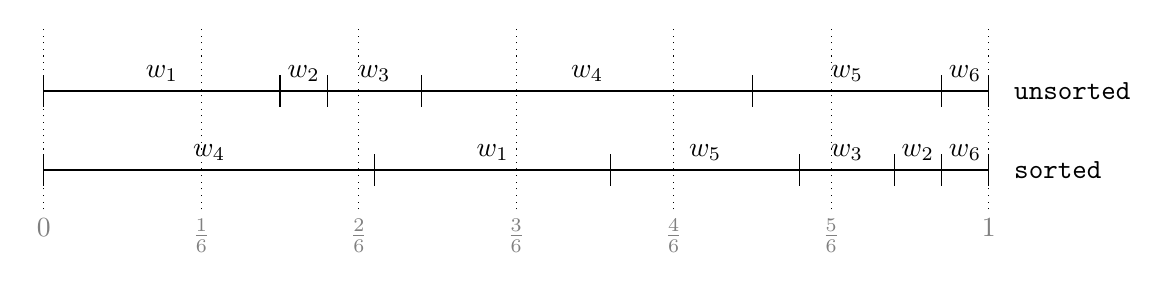
\begin{tikzpicture}
%% w = (0.25, 0.05, 0.10, 0.35, 0.20, 0.05)
%% vertical lines spaced 1/N apart
\draw[dotted] (0,-1.5) --(0,0.8);
\draw[dotted] (2,-1.5) --(2,0.8);
\draw[dotted] (4,-1.5) --(4,0.8);
\draw[dotted] (6,-1.5) --(6,0.8);
\draw[dotted] (8,-1.5) --(8,0.8);
\draw[dotted] (10,-1.5) --(10,0.8);
\draw[dotted] (12,-1.5) --(12,0.8);
%% labels for multiples of 1/N
\node[anchor=north, gray] at (0,-1.5) {$0$};
\node[anchor=north, gray] at (2,-1.5) {$\frac{1}{6}$};
\node[anchor=north, gray] at (4,-1.5) {$\frac{2}{6}$};
\node[anchor=north, gray] at (6,-1.5) {$\frac{3}{6}$};
\node[anchor=north, gray] at (8,-1.5) {$\frac{4}{6}$};
\node[anchor=north, gray] at (10,-1.5) {$\frac{5}{6}$};
\node[anchor=north, gray] at (12,-1.5) {$1$};
%% weight intervals, unsorted
\draw[thick] (0,0) -- (12,0);
\draw (0,-0.2) --(0,0.2);
\draw (3,-0.2) --(3,0.2);
\draw (3.6,-0.2) --(3.6,0.2);
\draw (4.8,-0.2) --(4.8,0.2);
\draw (9,-0.2) --(9,0.2);
\draw (11.4,-0.2) --(11.4,0.2);
\draw (12,-0.2) --(12,0.2);
%% weight labels, unsorted
\node[anchor=south] at (1.5,0) {$w_1$};
\node[anchor=south] at (3.3,0) {$w_2$};
\node[anchor=south] at (4.2,0) {$w_3$};
\node[anchor=south] at (6.9,0) {$w_4$};
\node[anchor=south] at (10.2,0) {$w_5$};
\node[anchor=south] at (11.7,0) {$w_6$};
%% weight intervals, sorted
\draw[thick] (0,-1) -- (12,-1);
\draw (0,-1.2) --(0,-0.8);
\draw (4.2,-1.2) --(4.2,-0.8);
\draw (7.2,-1.2) --(7.2,-0.8);
\draw (9.6,-1.2) --(9.6,-0.8);
\draw (10.8,-1.2) --(10.8,-0.8);
\draw (11.4,-1.2) --(11.4,-0.8);
\draw (12,-1.2) --(12,-0.8);
%% weight labels, sorted
\node[anchor=south] at (5.7,-1) {$w_1$};
\node[anchor=south] at (11.1,-1) {$w_2$};
\node[anchor=south] at (10.2,-1) {$w_3$};
\node[anchor=south] at (2.1,-1) {$w_4$};
\node[anchor=south] at (8.4,-1) {$w_5$};
\node[anchor=south] at (11.7,-1) {$w_6$};
%% labels sorted/unsorted
\node[anchor=west] at (12.2,0) {\texttt{unsorted}};
\node[anchor=west] at (12.2,-1) {\texttt{sorted}};
\end{tikzpicture}
\caption[Example where permuting weights can affect offspring counts]{An example in which permuting the weights can affect the conditional distribution of offspring counts under certain resampling schemes.
As in Figure~\ref{fig:inv_resampling}, $N=6$ and $w^{(1:6)} = (0.25,0.05,0.1,0.35,0.2,0.05)$.
The top row shows the weighted subintervals in the natural order, as in Figure~\ref{fig:inv_resampling}. 
The bottom row shows the partition corresponding to the same weights, but sorted in decreasing order. 
The dotted lines are spaced $1/N$ apart.
Under ``permutation-sensitive'' resampling schemes, the distribution of offspring counts differs depending on which partition is used.}
\label{fig:permutation_sensitivity}
\end{figure}

%\subsubsection{Sorting}
Related to this phenomenon, \textcite{gerber2017} prove some striking theoretical results concerning the effects of pre-sorting the particles. They show that sorting the particles in order of their states prior to resampling improves the rate of decay of resampling error from the usual $O(N^{-1})$ to $O(N^{1-\frac{1}{d}})$, where $d$ is the dimension of the state space. 
In dimension $d=1$, this supports the numerical results of \textcite{kitagawa1996}, who observed empirically that sorting improved the convergence rate from $O(N^{-1})$ to $O(N^{-2})$ when working in one dimension.

In dimension $d\geq2$ things are more complicated because there is no full ordering of the state space. \textcite{gerber2017} get around this by mapping the state space onto $[0,1]^d$ and sorting by the Hilbert curve. 
The variance reduction from sorting the particles diminishes as the dimension increases, so in practice this has to be weighed up against the $O(N\log N)$ cost of sorting.

Another remarkable result of \textcite{gerber2017} is that, when the particles are sorted by their states, systematic resampling admits some theoretical support that was lacking in the unsorted case.
Recall that the possibly pathological behaviour of systematic resampling was related to ``bad'' orderings of the weight intervals; sorting the particles evidently prevents this.

The intuition behind these results\seb{(I guess...)} is that sorting particles by their positions ensures that the stratified and systematic resampling schemes select parents from a good range of locations in state space. The sorting step prevents the sampled parents being concentrated in one small part of the state space purely by a chance ordering of the weight intervals.

These results are only relevant to resampling schemes based on inversion sampling with fairly evenly-spaced points. Notably, multinomial resampling is not affected by sorting, since it is invariant under permutations of the weight vector.
%\seb{I'm not sure about SSP; GCW imply that sorting is unnecessary in SSP because it's so great anyway, but they don't actually claim that SSP is unnaffected by sorting. My intuition is that it probably is affected, in some complex way.}




\subsubsection{Computational complexity}
All of the resampling algorithms discussed in Section~\ref{sec:examples_resamplingschemes} can be implemented in $O(N)$ operations.
%\seb{Even \texttt{star} and \texttt{SSP} and \texttt{branching}? If it turns out to differ depending on resampling scheme then include it as a column in Table~\ref{tab:resampling_properties}. --- I think we can't say for \texttt{branching} becaue it dpeends on implementation, but \textcite[Corollary 18]{crisan1999} seems to imply $O(N^2)$...? SSP is definitely $O(N)$.}
Considering the complexity of each operation, \textcite{hol2006} suggest that systematic resampling is fastest because it only requires one pseudo-random number generation, and multinomial resampling is slower than stratified resampling because of the transformations required (although this may depend on which method is used to sample the Uniform order statistics). Residual resampling is hard to compare directly because a random fraction of the operations are deterministic, so the number of pseudo-random numbers required is a random number between $0$ and $N-1$, but the authors' simulation experiments place it between multinomial and stratified resampling.

However, the analysis of per-particle cost is sensitive to the particular implementation of each resampling scheme, the system implementation of pseudo-random number generation and arithmetic operations, and the hardware used, so it is not clear how robust such comparisons are.




\subsubsection{Negative association}
Following \textcite{gerber2017}, we use the definition of negative association from \textcite{joag1983}.
\begin{defn}
Let $(Z_1, \dots, Z_n)$ be a collection of random variables. 
$Z_{1:n}$ are said to be \emph{negatively associated} if, for every disjoint pair of subsets $I, J \subseteq \{1,\dots,n\}$, for all real-valued coordinatewise non-decreasing functions $\varphi, \psi$ for which the covariance is well defined,
\begin{equation*}
\Cov \left[ \varphi( Z_I) , \psi(Z_J) \right] \leq 0 .
\end{equation*}
\end{defn}
\textcite{gerber2017} show that negative association of offspring counts is a desirable property which may be used, along with some other machinery, to establish certain weak convergence results for the resampled measures.

Multinomial counts are negatively associated \parencite[Section 3.1]{joag1983}, which implies that residual-multinomial resampling also satisfies this property.
\seb{Check that! Idea: deterministic parts have 0 correlation and the random parts are NA. Same goes for the other residual schemes mentioned below.}
\textcite{gerber2017} construct a counter-example to demonstrate that systematic resampling violates the negative association property.
For residual-systematic resampling, we can cook up a counterexample in the same spirit by taking $\varphi(x)=\psi(x)=\I{x=1}$, $I=\{1\}$, $J=\{3\}$ and considering a weight vector say $w^{(1:4)} = \frac{1}{8}(1,1,1,5)$ for $N=4$. Then the residual weights are $r^{(1:4)} = \frac{1}{4}(1,1,1,1)$ with $R=2$, so
\begin{align*}
\Cov \left[ \varphi( Z_I) , \psi(Z_J) \right]
&= \E[ \varphi( Z_I) \psi(Z_J) ] - \E[\varphi( Z_I) ] \E[\psi(Z_J) ] \\
&=\Prob[\nu^{(1)}=1, \nu^{(3)}=1] - \Prob[\nu^{(1)}=1] \Prob[\nu^{(3)}=1] \\
&= \frac{1}{2} - \frac{1}{2} \cdot \frac{1}{2} 
= \frac{1}{4}
>0 ,
\end{align*}
since $\nu^{(3)}=1$ if and only if $\nu^{(1)}=1$. 
So residual-systematic resampling also violates the negative association property.

\textcite{gerber2017} also mention some resampling schemes that do result in negatively associated counts: stratified resampling, and by implication residual-stratified resampling; star resampling (see the remark at the end of \textcite[Section 3.2]{gerber2017}), and by implication residual-star resampling.
The authors go on to introduce the SSP resampling scheme, which yields negatively associated offspring counts by construction.

These results are summarised in Table~\ref{tab:resampling_properties}.
The MVB algorithm does not enforce negative association, so this property depends on the particular implementation, and as such is left blank in Table~\ref{tab:resampling_properties}.







\subsubsection{Star discrepancy}
The \emph{star discrepancy} is a measure of the regularity of a given set of points $u_{1:N}$ in the unit hypercube. For our purposes it is sufficient to define the star discrepancy in one dimension, as in \textcite[Definition 1.2]{kuipers1974}:
\begin{equation}\label{eq:defn_stardiscrepancy}
D^\star (u_1, \dots, u_N)
:= \sup_{u \in [0,1]} | d(u) |
:= \sup_{u \in [0,1]} \left| u - \frac{1}{N} \sum_{i=1}^N \I{u_i \leq u} \right| .
\end{equation}
The quantity inside the supremum is the difference between the empirical CDF of the observed points $u_{1:N}$ and the CDF of the Uniform distribution on $[0,1]$.
Thus $D^\star$ measures, in a certain sense, how far the points are from being uniformly spaced.

\begin{figure}[ht]
\centering
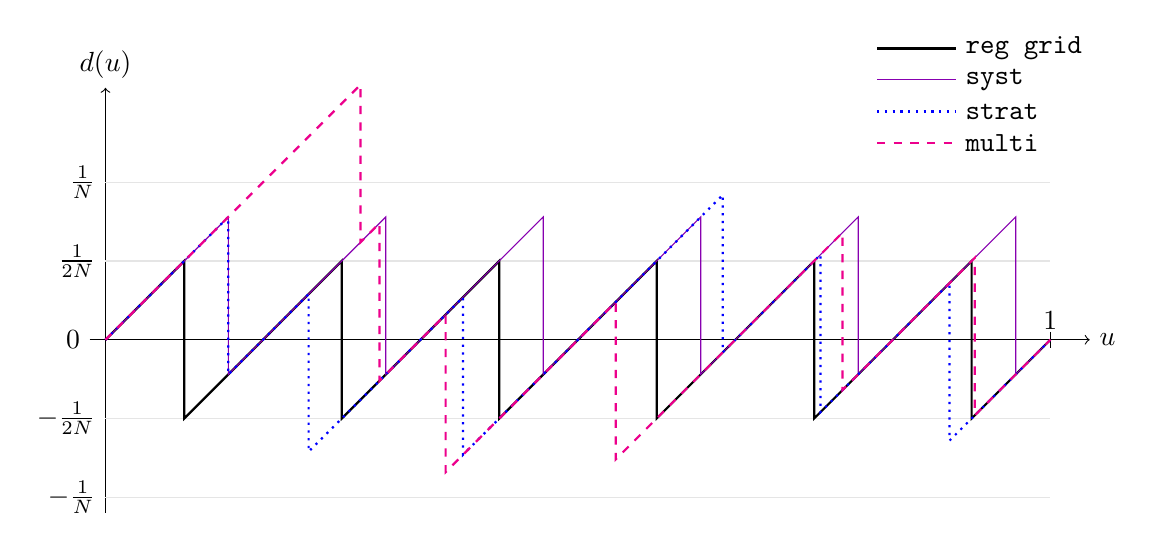
\begin{tikzpicture}
%% axes
\draw[->] (-0.2,0)--(12.5,0);
\draw[->] (0,-2.2)--(0,3.2);
\draw (12,0.1)--(12,-0.1);
\draw[gray!20] (0,1)--(12,1);
\draw[gray!20] (0,-1)--(12,-1);
\draw[gray!20] (0,2)--(12,2);
\draw[gray!20] (0,-2)--(12,-2);
%% axis labels
\node[anchor=west] at (12.5,0) {$u$};
\node[anchor=south] at (0,3.2) {$d(u)$};
\node[anchor=south] at (12,0) {$1$};
\node[anchor=east] at (-0.2,0) {$0$};
\node[anchor=east] at (0,1) {$\frac{1}{2N}$};
\node[anchor=east] at (0,-1) {$-\frac{1}{2N}$};
\node[anchor=east] at (0,2) {$\frac{1}{N}$};
\node[anchor=east] at (0,-2) {$-\frac{1}{N}$};
%% regular grid points
\draw[thick] (0,0)--(1,1)--(1,-1)--(3,1)--(3,-1)--(5,1)--(5,-1)--(7,1)--(7,-1)--(9,1)--(9,-1)--(11,1)--(11,-1)--(12,0);
%% systematic grid points, u as in Figure~\ref{fig:inv_resampling}
\draw[violet] (0,0)--(1.56,1.56)--(1.56,-0.44)--(3.56,1.56)--(3.56,-0.44)--(5.56,1.56)--(5.56,-0.44)--(7.56,1.56)--(7.56,-0.44)--(9.56,1.56)--(9.56,-0.44)--(11.56,1.56)--(11.56,-0.44)--(12,0);
%% stratified grid points, ditto
\draw[thick, blue, dotted] (0,0)--(1.56,1.56)--(1.56,-0.44)--(2.58,0.58)--(2.58,-1.42)--(4.54,0.54)--(4.54,-1.46)--(7.84,1.84)--(7.84, -0.16)--(9.08,1.08)--(9.08,-0.92)--(10.72,0.72)--(10.72,-1.28)--(12,0);
%% multinomial points, ditto
\draw[thick, magenta, dashed] (0,0)--(3.24,3.24)--(3.24,1.24)--(3.48,1.48)--(3.48,-0.52)--(4.32,0.32)--(4.32,-1.68)--(6.48,0.48)--(6.48,-1.52)--(9.36,1.36)--(9.36,-0.64)--(11.04,1.04)--(11.04,-0.96)--(12,0);
%% legend
\draw[thick, magenta, dashed] (9.8,2.5)--(10.8,2.5);
\node[anchor=west] at (10.8,2.5) {\texttt{multi}};
\draw[thick, blue, dotted] (9.8,2.9)--(10.8,2.9);
\node[anchor=west] at (10.8,2.9) {\texttt{strat}};
\draw[violet] (9.8,3.3)--(10.8,3.3);
\node[anchor=west] at (10.8,3.3) {\texttt{syst}};
\draw[thick] (9.8,3.7)--(10.8,3.7);
\node[anchor=west] at (10.8,3.7) {\texttt{reg grid}};
\end{tikzpicture}
\caption[Star discrepancy for multinomial, stratified and systematic resampling]{Plot of the function inside the absolute value in \eqref{eq:defn_stardiscrepancy}, for four different point sets. The points $u_{1:6}$ used are the same as in Figure~\ref{fig:inv_resampling}.\\
The solid black line corresponds to the regular grid, which achieves the minimal discrepancy $1/(2N)$, but cannot be used for resampling.
The star discrepancy of stratified and systematic points varies between $1/(2N)$ and $1/N$ depending on the realisation. In this example, the star discrepancy of the systematic points is $0.78/N$ and of the stratified points is $0.92/N$.
The star discrepancy of standard multinomial resampling (that is, i.i.d.\ Uniform points) can be arbitrarily close to $1$ for ``bad'' realisations; in this example it is $1.62/N$.}
\label{fig:star_discrepancy}
\end{figure}

Star discrepancy is used in quasi-Monte Carlo, where ``low-discrepancy'' points are used in place of Uniform random numbers to decrease the variance of Monte Carlo estimates.
We have noted already that resampling can itself be viewed as a Monte Carlo procedure.
From this point-of-view, stratified and systematic resampling are quasi-Monte Carlo implementations of multinomial resampling, since they provide ``more regular'' point sets to be used in inversion sampling.

In one dimension, the lowest-discrepancy point set is the regular grid $\frac{1}{2N}(1, 3, \dots, 2N-1)$, which has star discrepancy $\frac{1}{2N}$ \parencite[see for example][Corollary 1.2]{kuipers1974}.
However, resampling based on a deterministic point set cannot be unbiased since the resulting parental indices are conditionally deterministic given the weights.
Systematic resampling amounts to a randomisation of the regular grid, shifting each grid point by a random amount $u \sim \Unif[0,1/N]$. This yields star discrepancy $D^\star = \max\{u, \frac{1}{N} -u\}$, which is between $1/(2N)$ and $1/N$ almost surely.
The point sets generated in stratified resampling also have star discrepancy between $1/(2N)$ and $1/N$, where the exact value depends on the realisation.
This certainly seems to improve on independent uniform points which can have star discrepancy arbitrarily close to $1$, the maximum possible value, albeit with diminishing probability as $N$ increases.
Figure~\ref{fig:star_discrepancy} illustrates how the star discrepancy is computed, and how it compares between these sampling methods.


%\subsubsection{Optimal resampling}
%\textcite{crisan1999} introduce another resampling scheme based on a branching process, which they show to be optimal in some sense. However, their algorithm is not widely used in practice because it is much more complicated to implement than alternatives like systematic resampling which perform just as well empirically, and share some of its optimality properties \parencite{bain2008}. 
%\seb{Possibly add an ``optimality'' column in Table~\ref{tab:resampling_properties} containing in what sense a scheme might be considered optimal.}



\begin{landscape}
\begin{table}[ht]
\centering
\begin{tabular}{ l | c c c c c c c c }
\hline\hline
& \thead{support of $\nu_t^{(i)}$ given
            \\ $ \frac{K}{N} \leq w_t^{(i)} < \frac{K+1}{N}$} 
        & \thead{$\sup_w$\\ $|\nu_t^{(i)} - Nw_t^{(i)}|$}
        & \thead{upper\\ bound on \\ $\V[\nu_t^{(i)}]$}
        & \thead{stochastic\\ rounding?}       
        & \thead{degenerate if\\ $w_t^{(1:N)} =$\\ $\frac{1}{N}(1,\dots,1)$?} 
        & \thead{sensitive to\\ permutations\\ of weights?} 
        & \thead{PRNG\\ calls}
        & \thead{neg.\\ assoc.?} \\
\hline
\texttt{multi} & $\{0,\dots,N\}$ & $N$ & $N/4$ & $\times$ & $\times$ 
        & $\times$ & $N$ & $\checkmark$ \\
\texttt{star} & $\{0, N\}$ & $N$ & $N^2/4$ & $\times$ & $\times$ 
        & $\times$ & $1$ & $\checkmark$? \\
\texttt{strat} & $\{K-1, K, K+1, K+2\}$ & $2$ & $2$ & $\times$ & $\checkmark$ 
        & $\checkmark$ & $N$ & $\checkmark$ \\
\texttt{syst} & $\{K, K+1\}$ & $1$ & $1/4$ & $\checkmark$ & $\checkmark$ 
        & $\checkmark$ & $1$ & $\times$ \\
\texttt{res-multi} & $\{K,\dots,N\}$ & $N-1$ & $1$ & $\times$ & $\checkmark$ 
        & $\times$ & $\leq N-1$ & $\checkmark$ \\
\texttt{res-star} & $\{K, N\}$ & $N-1$ & $N$ & $\times$ & $\checkmark$ 
        & $\times$ & $1$ & $\checkmark$? \\
\texttt{res-strat} & $\{K, K+1, K+2\}$ & $2$ & $1/2$ & $\times$ & $\checkmark$ 
        & $\checkmark$ & $\leq N-1$ & $\checkmark$ \\
\texttt{res-syst} & $\{K, K+1\}$ & $1$ & $1/4$ & $\checkmark$ & $\checkmark$ 
        & $\checkmark$ & $1$ & $\times$ \\
\texttt{ssp} & $\{K, K+1\}$ & $1$ & $1/4$ & $\checkmark$ & $\checkmark$ 
        & $\checkmark$? & $\leq N$ & $\checkmark$ \\
\texttt{mvb} & $\{K, K+1\}$ & $1$ & $1/4$ & $\checkmark$ & $\checkmark$ 
        & & & \\
\hline\hline
\end{tabular}
\caption[Properties of resampling schemes]{Summary of some of the properties of resampling schemes explored in Section~\ref{sec:resampling_properties}. The abbreviated names for the resampling schemes are explained in Table~\ref{tab:resampling_abbrevs}. Some properties are not specified for \texttt{branching} bacuase they depend on the particular implementation.}
\label{tab:resampling_properties}
\end{table} 
\end{landscape}
 
 
 

\subsection{Stochastic rounding}
\label{sec:SRs}

\begin{defn}\label{defn:stochround}
 Let $X=(X_1,\dots,X_N)$ be a $\mathbb{R}_+^N$-valued random variable. Then $Y=(Y_1,\dots,Y_N) \in \mathbb{N}^N$ is a \emph{stochastic rounding} of $X$ if each element $Y_i$ takes values
\begin{equation*}
Y_i \mid X_i =
\begin{cases}
 \lfloor X_i \rfloor & \text{with probability } 1- X_i+ \lfloor X_i \rfloor \\
  \lfloor X_i \rfloor +1 & \text{with probability } X_i- \lfloor X_i \rfloor .
\end{cases}
\end{equation*}
\end{defn}

By construction, $\E(Y_i) = X_i$ for each $i$. Taking $X$ to be $N$ times the vector of particle weights, we can therefore use stochastic rounding to construct a valid resampling scheme, under the further constraint that $Y_1 + \dots + Y_N = N$.
Several ways to enforce this constraint on the joint distribution have been proposed, including systematic resampling, residual resampling with systematic residuals, and SSP resampling.

Explicitly, the offspring counts are marginally distributed according to 
\begin{equation*}
\nu_t^{(i)} \mid w_t^{(i)}
\eqdist \flnw + \Bern( Nw_t^{(i)} - \flnw ) .
\end{equation*}

Some of the properties discussed earlier are common to every stochastic rounding scheme. 
Since all such schemes give offspring counts with the same marginal distributions, properties such as the marginal offspring variance are common to all stochastic roundings. Indeed it is easy to see that the marginal variance of the offspring counts, $\V[ \nu_t^{(i)} \mid w_t^{(i)} ]$ is as small as possible under the constraint of unbiasedness, and as such this is sometimes referred to as minimal-variance resampling.
By definition, the support of an offspring count $\nu_t^{(i)}$ given that the associated weight lies in the interval $K/N \leq w_t^{(i)} < (K+1)/N$ is $\{ K, K+1\}$. 
All stochastic roundings are also degenerate when the weights are all equal, i.e.\ $w_t^{(1:N)} = (1,\dots, 1)/N$ implies $\nu_t^{(1:N)}=(1,\dots,1)$ almost surely.





\section{Conditional SMC}
\label{sec:condSMC}
%\seb{Be consistent with upper/lower case letters: $X,x$ etc.}\\
\textcite{andrieu2010} propose a number of ``particle MCMC'' algorithms, which combine SMC with MCMC in order to improve performance in certain situations.
One of their algorithms, the \emph{particle Gibbs} sampler \parencite[Section 2.4.3]{andrieu2010}, is of particular interest in the current work. For one thing, genealogies are particularly critical to its performance, and for another, the particle update uses a variant SMC algorithm which alters the distribution of genealogies.

In this section, we first introduce the particle Gibbs algorithm and the conditional SMC update, then discuss how ancestral degeneracy impacts the performance of particle Gibbs and how ancestor sampling mitigates this.




\subsection{Particle Gibbs}
\label{sec:particleGibbs}
To motivate the particle Gibbs algorithm, we introduce a parametrised state space model and explain how combining SMC updates with MCMC sampling allows us to tackle the related inferences effectively.
The particle Gibbs algorithm can be applied much more broadly, but this application is particularly intuitive and exhibits all the features of interest to our genealogical study.

Consider a parametrised state space model of the form
\begin{align*}
\theta &\sim p(\cdot) & \\
X_0 &\sim \mu^\theta(\cdot) & \\
X_{t+1} \mid X_{t} &\sim K_{t+1}^\theta(\cdot \mid X_{t}) &\text{for } t=0,\dots, T-1 \\
Y_t \mid X_t &\sim g_t^\theta(\cdot \mid X_t) &\text{for } t=0,\dots, T
\end{align*}
exactly like \eqref{eq:SSM_spec} except that the specification is now parametrised by $\theta$ (which may be multi-dimensional), and we place a prior distribution on $\theta$. 
As usual, $p$, $\mu^\theta$, $(K_t^\theta)$ and $(g_t^\theta)$ are part of the model and are assumed to be known but not necessarily tractable.

Suppose that, given some data $y_{0:T}$, we wish to generate Monte Carlo samples from the joint posterior distribution of $X_{0:T}$ and $\theta$. (Even if we are only interested in inferring $\theta$, for instance, it is often more practical to target the joint posterior and then marginalise.)
Notice that we are now working with a finite time horizon $T\in\mathbb{N}$. The inference of interest here is not inherently sequential; we are building an MCMC algorithm to sample from a single target distribution which happens to include some sequentially correlated components.


The conditional dependence structure of the model invites the use of a (partially-collapsed) Gibbs sampler, sampling alternately from the conditional distributions $p(\theta \mid x_{0:T}, y_{0:T})$ and $p(x_{0:T} \mid \theta, y_{0:T})$.
The $\theta$ update,
\begin{equation*}
p(d\theta \mid x_{0:T}, y_{0:T}) \propto p(d\theta) p(x_{0:T}, y_{0:T} \mid \theta) ,
\end{equation*}
is often quite straightforward, if not analytically then by employing a Metropolis-Hastings step based on the current sampled values of $\theta$ and $x_{0:T}$. 
The $X$ update, meanwhile, is high-dimensional with strong sequential correlations: exactly the situation in which one might use SMC. 
For the $X$ update, we need a sample from
\begin{equation}\label{eq:PG_Xposterior}
p(dx_{0:T} \mid \theta, y_{0:T}) 
\propto \mu^\theta(dx_0) g_0^\theta(y_0\mid x_0) \prod_{s=1}^T K_s^\theta(dx_s \mid x_{s-1}) g_s^\theta(y_s \mid x_s) ,
\end{equation}
which can be obtained by running an SMC smoother then sampling one trajectory from its output in proportion to the associated weight.

However, the Markov chain associated to the procedure just described does not admit $p(x_{0:T},\theta \mid y_{0:T})$ as an invariant distribution. It \emph{approximately} targets this distribution, with some bias.
A Gibbs sampler targeting $p(x_{0:T},\theta \mid y_{0:T})$ exactly can be constructed by replacing the SMC step with a \emph{conditional SMC} step, which takes into account the value of $x_{0:T}$ sampled at the previous iteration, as well as the observations and the current value of $\theta$.

A conditional SMC algorithm for this scenario is presented in Algorithm~\ref{alg:condSMC}.
In contrast to Algorithm~\ref{alg:SMC}, the input now includes $x_{0:T}^\star$ and $a_{0:T}^\star$, which encode the states and parental indices, respectively, of the \emph{immortal trajectory} (so called because it ``survives'' the SMC run with probability one). Within a particle Gibbs algorithm, the immortal trajectory is set to the trajectory sampled at the previous iteration.
The resampling step now assigns the immortal offspring to the immortal parent deterministically, and the state of the immortal particle is also updated deterministically rather than via the Markov kernel.
As in standard SMC, there is a choice of \textsc{resample} procedures, but some care is needed to ensure the correct treatment of the immortal particle \parencite[for details see e.g.][]{lee2019}.

\begin{algorithm}[ht]
\vspace*{10pt}
\DontPrintSemicolon
\KwIn{$T, N, \mu^\theta, (K_t^\theta), (g_t^\theta), y_{0:T}, x_{0:T}^\star, a_{0:T}^\star$}
Set $X_0^{(a_0^\star)} \gets x_0^\star$\;
\lFor{$i \in \{1,\dots,N\} \setminus a_0^\star$}{
	Sample $X_0^{(i)} \sim \mu(\cdot)$
}
\lFor{$i \in \{1,\dots, N\}$}{
		$w_{0}^{(i)} \gets \left\{ {\sum_{j=1}^N g_0^\theta(y_0 \mid X_0^{(j)})}\right \}^{-1}{g_0^\theta(y_0 \mid X_0^{(i)})} $
}                
\For{$t \in \{1,\dots, T\}$}{
	Set $a_{t-1}^{(a_{t}^\star)} \gets a_{t-1}^\star$, 	$X_{t}^{(a_{t}^\star)} \gets x_{t}^\star$\;
        Sample $a_{t-1}^{(1:N)}\setminus a_{t-1}^\star \sim \textsc{resample}(\{1,\dots,N\}, w_{t-1}^{(1:N)})$\;
	\lFor{$i \in \{1,\dots,N\} \setminus a_t^\star$}{
		Sample $X_{t}^{(i)} \sim K_{t}^\theta( \cdot \mid X_{t-1}^{(a_{t-1}^{(i)})} )$
	}
    	\lFor{$i \in \{1,\dots, N\}$}{	
		$w_{t}^{(i)} \gets \Big\{ {\sum_{j=1}^N g_{t}^\theta(y_{t} \mid X_{t}^{(j)}) }\Big\}^{-1} g_{t}^\theta(y_{t} \mid X_{t}^{(i)}) $
	}          
}
\vspace*{10pt}
\caption[Conditional sequential Monte Carlo for a parametrised state space model]{Conditional sequential Monte Carlo for a parametrised state space model. The immortal particle at each generation has its new state and parental index set deterministically according to the values of $x_{0:T}^\star$ and $a_{0:T}^\star$ given as input.}
\label{alg:condSMC}
\end{algorithm}
The complete particle Gibbs algorithm for this example then consists of alternately sampling from the full conditional distribution of $\theta$ (e.g.\ using a Metropolis-Hastings update) and sampling a trajectory $(x_{0:T}, a_{0:T})$ using conditional SMC. See \textcite[Section 2.4.3]{andrieu2010} for more details.




\subsection{Ancestral degeneracy in particle Gibbs}
We have seen in Section~\ref{sec:SMC_genealogies} that the phenomenon of ancestral degeneracy can severely affect the performance of SMC algorithms, particularly in smoothing applications.
The SMC update of particle Gibbs is a smoothing problem, however it requires only one sampled trajectory from the smoothing distribution, so one might imagine that we are safe from the curse of ancestral degeneracy.
In fact, the loss of ancestors causes a different problem for particle Gibbs: it prevents some components of the Markov chain being refreshed, so that the chain mixes slowly.

To see this, consider the illustration in Figure~\ref{fig:PG_ancdegen}, which shows the smoothing trajectories generated by a conditional SMC update at some iteration $r$. The thick black line is the immortal trajectory given as input, that is, the trajectory sampled by the conditional SMC update at iteration $r-1$. Backwards in time, the sampled trajectories quickly coalesce until at time $20$ all of the trajectories have coalesced. The common trajectory from time $0$ to $20$ must necessarily be part of the immortal trajectory.
A new trajectory (highlighted in purple) is then sampled among the $N$ generated trajectories. Whichever trajectory we sample, it will certainly overlap with the previously sampled trajectory at least from time $0$ to $20$.

\begin{figure}[ht]
\centering
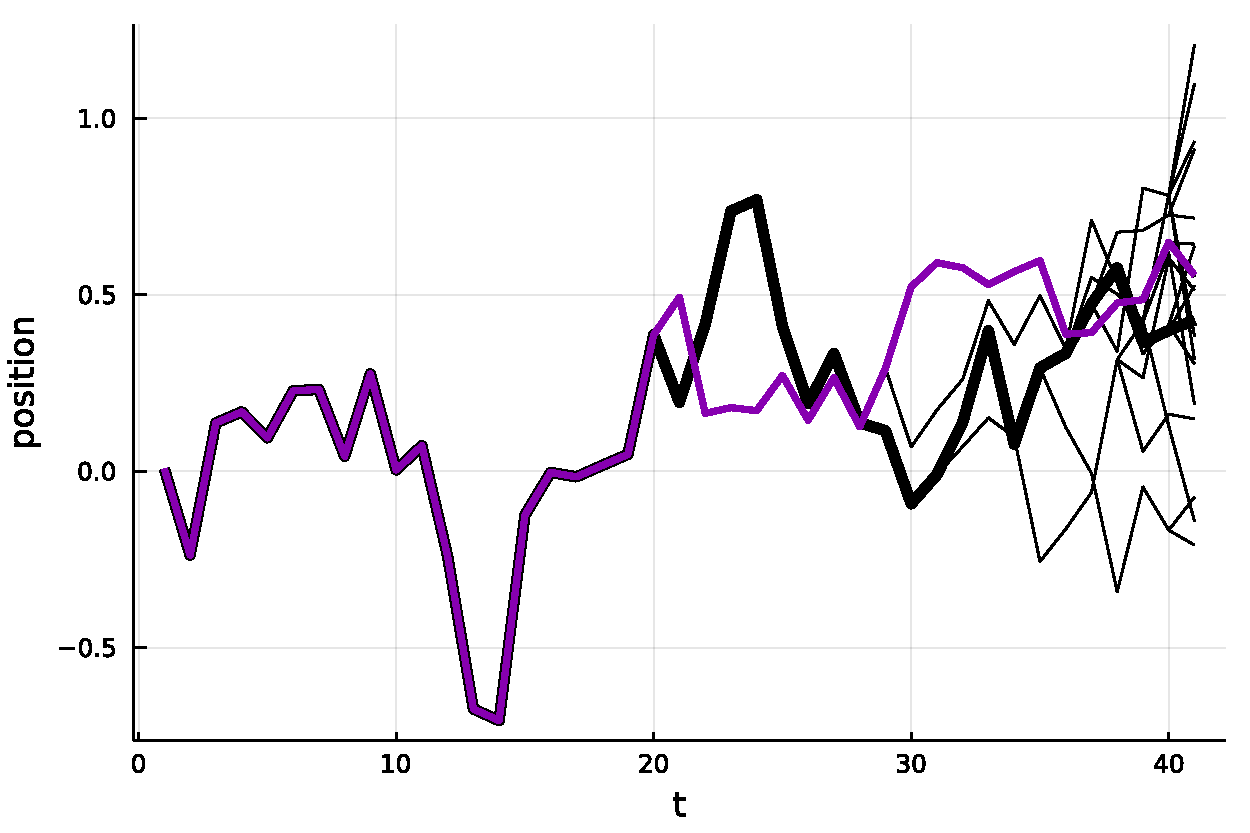
\includegraphics[width=0.8\textwidth]{../plots/PG_degen.pdf}
\caption[Ancestral degeneracy in particle Gibbs]{Illustration of how ancestral degeneracy causes particle Gibbs to mix slowly on some components. The thick black line is the immortal trajectory, i.e.\ the sampled trajectory from the previous iteration. Other lines are all of the trajectories generated by conditional SMC. One of these (highlighted in purple) is the sampled trajectory at the current iteration. Due to ancestral degeneracy, the current sample (purple) coincides with the previous sample (thick black) up to time 20, so the components $x_{0:20}$ are not updated in this iteration.}
\label{fig:PG_ancdegen}
\end{figure}

At the next iteration the newly sampled trajectories will again coalesce onto the immortal trajectory, and this behaviour is repeated. 
If $T$ is too large with respect to $N$, the early part of the trajectory will very rarely be updated, so the corresponding states will mix very slowly.
For further intuition on this phenomenon the reader is directed to \textcite[Section 5.4]{lindsten2013}.
%\seb{Also include a plot showing sticky realisations from a sequence of consecutive draws?}
%\seb{If the immortal trajectory is not ``typical'' of the target smoothing distribution, then the new lineages tend not to degenerate very quickly onto the immortal lineage, which would solve this problem. However, since the immortal trajectory is supposed to be (approaching) a sample from the target, this is not much comfort. Perhaps if perturbing $\theta$ profoundly changes the model? But I don't think that kind of instability is desirable either.}

The meaning of $T$ ``too large'' here depends on the model and the type of SMC update used, but typically $T$ is determined by the application and $N$ is limited by computational resources, so we may not be able to control their relative size. The other brute-force approach would be to increase the number of iterations of the MCMC algorithm, but this too is infeasible on a limited computational budget.
It is therefore worth investing some effort to find an alternative solution to the problem of ancestral degeneracy within particle Gibbs.





\subsection{Ancestor sampling}\label{sec:ancsamp}
An effective solution (where it is possible to implement it) was proposed by \textcite{whiteley2010} and is known as \emph{ancestor sampling}.
It consists of a simple modification to the resampling step within the conditional SMC algorithm. 
In the basic algorithm with multinomial resampling, at each time step the non-immortal particles are resampled by multinomial resampling according to their weights, while the immortal offspring is deterministically assigned to the immortal parent. That is, at time $t$, for each $i \in \{1,\dots, N\}$,
\begin{equation*}
\Prob[a_t^{(j)} = i \mid X_{0:t}^{(1:N)}, x_{0:T}^\star, a_{0:T}^\star ] 
\propto \begin{cases}
w_t^{(i)} & j \text{ non-immortal} \\
\I{i = a_t^\star} & j \text{ immortal} .
\end{cases}
\end{equation*}

Ancestor sampling combines the resampling step with a backward simulation step for the immortal particle. Instead of deterministically inheriting the ``correct'' parent, the immortal particle samples its parent among all $N$ possible parents.
This is justified in the same way as backwards simulation in general (Section~\ref{sec:anc_degen}), provided the ancestor sampling probabilities are chosen correctly, although we now apply the backwards sampling step to the immortal trajectory only.
Ancestor sampling can also be implemented for other choices of \textsc{resample}, using the same backward simulation probabilities (but of course the resampling probabilities for non-immortal particles will be different, and there may be some additional dependence between parental indices). For simplicity we here restrict ourselves to multinomial resampling.

\begin{algorithm}[ht]
\vspace*{10pt}
\DontPrintSemicolon
\KwIn{$T, N, \mu^\theta, (K_t^\theta), (g_t^\theta), y_{0:T}, x_{0:T}^\star, a_{0:T}^\star$}
Set $X_0^{(a_0^\star)} \gets x_0^\star$\;
\lFor{$i \in \{1,\dots,N\} \setminus a_0^\star$}{
	Sample $X_0^{(i)} \sim \mu^\theta(\cdot)$
}
\lFor{$i \in \{1,\dots, N\}$}{
		$w_{0}^{(i)} \gets  \left\{ {\sum_{j=1}^N g_0^\theta(y_0 \mid X_0^{(j)})}\right \}^{-1}{g_0^\theta(y_0 \mid X_0^{(i)})} $
}                
\For{$t \in \{1,\dots, T\}$}{
	Set $X_{t}^{(a_{t}^\star)} \gets x_{t}^\star$\;
	Sample $a_{t-1}^{(a_{t}^\star)} \sim \Cat\left( \{1,\dots,N\}, w_{t-1}^{(1:N)} q_{t}^\theta(x_{t}^\star \mid X_{t-1}^{(1:N)}) \right)$\;
        Sample $a_{t-1}^{(1:N)}\setminus a_{t-1}^\star \sim \textsc{resample}(\{1,\dots,N\}, w_{t-1}^{(1:N)})$\;
	\lFor{$i \in \{1,\dots,N\} \setminus a_t^\star$}{
		Sample $X_{t}^{(i)} \sim q_{t}^\theta( \cdot \mid X_{t-1}^{(a_{t-1}^{(i)})} )$
	}
    	\lFor{$i \in \{1,\dots, N\}$}{	
		$w_{t}^{(i)} \gets \Big\{ {\sum_{j=1}^N g_{t}^\theta( y_{t} \mid X_{t}^{(j)}) }\Big\}^{-1} g_{t}^\theta( y_{t} \mid X_{t}^{(i)}) $
	}          
}
\vspace*{10pt}
\caption[Conditional sequential Monte Carlo with ancestor sampling]{Conditional sequential Monte Carlo with ancestor sampling for a parametrised state space model. The parent of the immortal particle is updated at each iteration via an on-line backward simulation step. The second parameter of the Categorical variable should be interpreted element-wise.}
\label{alg:condSMC_ancsamp}
\end{algorithm}
Assume that the smoothing distributions admit densities, that is $\mu^\theta(\cdot)$ and $K_t^\theta(\cdot\mid x)$ admit densities for all $x,t$. Denote the density of $K_t^\theta$ by $q_t^\theta$. Define the trajectories $X_{t, 0:t}^{(i)}$ (for any $t,i$) as in Section~\ref{sec:SMC_FK}, starting from $X_{t,t}^{(i)} := X_t^{(i)}$ and tracing back the states of the parents via $X_{t,s}{(i)} = X_{t,s+1}^{( a_t^{(i)} )}$.
Then the correct resampling probabilities are, for each $i$,
\begin{equation}\label{eq:ancsamp_probs}
\Prob[a_t^{(j)} = i \mid X_{0:t}^{(1:N)}, x_{0:T}^\star, a_{0:T}^\star ] 
\propto \begin{cases}
w_t^{(i)} & j \text{ non-immortal}\\
w_t^{(i)} \frac{
        p( (X_{t,0:t}^{(i)}, x_{t+1:T}^\star) \mid \theta, y_{0:T} )}
        {p( X_{t,0:t}^{(i)} \mid \theta, y_{0:t} ) } 
        & j \text{ immortal} .
\end{cases}
\end{equation}
The ratio of densities can be interpreted as the conditional probability that the whole trajectory is the concatenation of $X_{t,0:t}^{(i)}$ with $x_{t+1:T}^\star$, given that its first $t+1$ states are $X_{t,0:t}^{(i)}$.
To simplify the ratio, use \eqref{eq:PG_Xposterior} to write
\begin{equation*}
p( X_{t,0:t}^{(i)} \mid \theta, y_{0:t} )
\propto \mu^\theta( X_{t,0}^{(i)} ) g_0^\theta( y_0 \mid X_{t,0}^{(i)} ) 
        \prod_{s=1}^{t} q_s^\theta( X_{t,s}^{(i)} \mid X_{t,s-1}^{(i)} ) 
        g_s^\theta( y_s \mid X_{t,s}^{(i)} )
\end{equation*}
and %\seb{actually, this explicit trajectory notation is going to make all this much heavier... but perhaps it's worth it for the clarity?}
\begin{align*}
&p( (X_{t,0:t}^{(i)}, x_{t+1:T}^\star) \mid \theta, y_{0:T} ) \\
&\qquad \propto \mu^\theta( X_{t,0}^{(i)} ) g_0^\theta( y_0 \mid X_{t,0}^{(i)} ) 
        \left\{ \prod_{s=1}^{t} q_s^\theta( X_{t,s}^{(i)} \mid X_{t,s-1}^{(i)} )
        g_s^\theta( y_s \mid X_{t,s}^{(i)} ) \right\} \\
    &\hspace{2cm}\times q_{t+1}^\theta( x_{t+1}^\star \mid X_{t,t}^{(i)} ) 
        g_{t+1}^\theta( y_{t+1} \mid x_{t+1}^\star )
        \left\{ \prod_{s=t+2}^T q_s^\theta(x_s^\star \mid x_{s-1}^\star)
        g_s^\theta(y_s \mid x_s^\star) \right\} .
\end{align*}
The ratio then becomes
%\seb{I think the first proportionality hides the likelihood ratio $p(y_{0:T}|\theta)/p(y_{0:t-1}|\theta)$ --- see \eqref{eq:PG_Xposterior} --- it might make things clearer if I keep such constants explicit for longer?}
\begin{align*}
&\frac{p( ( X_{t,0:t}^{(i)}, x_{t+1:T}^\star ) \mid \theta, y_{0:T} )}
        {p( X_{t,0:t}^{(i)} \mid \theta, y_{0:t} ) } \\
&\qquad\qquad\propto q_{t+1}^\theta( x_{t+1}^\star \mid X_{t,t}^{(i)} ) 
        g_{t+1}^\theta( y_{t+1} \mid x_{t+1}^\star )
        \prod_{s=t+2}^T q_s^\theta( x_s^\star \mid x_{s-1}^\star ) 
        g_s^\theta( y_s \mid x_s^\star ) \\
&\qquad\qquad\propto q_{t+1}^\theta( x_{t+1}^\star \mid X_{t,t}^{(i)} )
        = q_{t+1}^\theta( x_{t+1}^\star \mid X_{t}^{(i)} )  .
\end{align*}
The probabilities in \eqref{eq:ancsamp_probs} become
\begin{equation}\label{eq:ancsamp_probs_simplified}
\Prob[a_t^{(j)} = i \mid X_{0:t}^{(1:N)}, x_{0:T}^\star, a_{0:T}^\star ] 
\propto \begin{cases}
w_t^{(i)} & j \text{ non-immortal}\\
w_t^{(i)} q_{t+1}^\theta( x_{t+1}^\star \mid X_{t}^{(i)} ) & j \text{ immortal} .
\end{cases}
\end{equation}
The conditional SMC algorithm with this adaptation is presented in Algorithm~\ref{alg:condSMC_ancsamp}.

We see that, in order to do ancestor sampling, we need a stronger assumption on the Markov kernels than was required to simply run the conditional SMC algorithm: we now require that, for each $t$, $K_t^\theta$ admits a density $q_t^\theta$ and that $q_t^\theta(\cdot \mid x)$ can be evaluated pointwise for any $x$, whereas previously we only needed to draw samples from $K_t^\theta(\cdot\mid x)$ for any $x$.
This additional requirement rules out ancestor sampling in some applications.

Recall that the usual backward simulation procedure requires a full forward pass to calculate the future states before the backward simulation probabilities can be computed. Ancestor sampling, on the other hand, does not require a forward pass because it only computes backward simulation probabilities for the immortal trajectory, for which all the future states are known in advance. This means that the additional computational cost of implementing ancestor sampling is negligible.




\subsubsection{Why ancestor sampling works}
We know that complete backward simulation eradicates ancestral degeneracy by sampling each lineage independently (Section~\ref{sec:anc_degen}).
But here we are only backward-simulating one of the $N$ particles, leaving the other $N-1$ lineages to coalesce as usual. So how does this help?

Recall that in particle Gibbs ancestral degeneracy is not itself a problem, because we only require a single sample from the smoothing distribution. 
The problem is that the consecutive samples are highly correlated, because of  the repeated coalescence onto the immortal lineage.
The contribution of ancestor sampling is to break up the immortal trajectory so that it no longer appears among the lineages; see Figure~\ref{fig:whyASworks}. While the non-immortal trajectories may still coalesce, they no longer preferentially coalesce onto the immortal trajectory. 
In turn, the sampled trajectory that is output does not overlap unduly with the immortal trajectory that was the previous output, and this completely solves the problem of the slow-mixing particle Gibbs chain.

\begin{figure}[ht]
\centering
\subfloat[without ancestor sampling]{
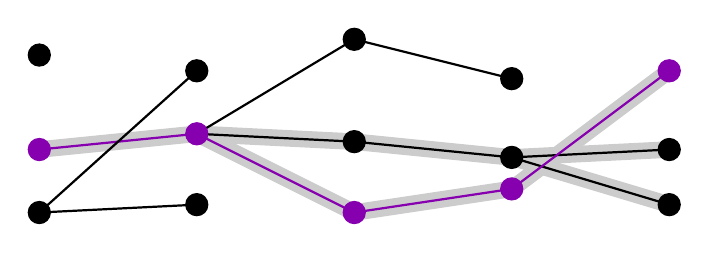
\begin{tikzpicture}
% highlight lineage 1 (immortal lineage)
\draw[line width=6pt, gray!40] (0,0.8)--(2,1);
\draw[line width=6pt, gray!40] (2,1)--(4,0);
\draw[line width=6pt, gray!40] (4,0)--(6,0.3);
\draw[line width=6pt, gray!40] (6,0.3)--(8,1.8);
% highlight lineage 2
\draw[line width=6pt, gray!40] (2,1)--(4,0.9);
\draw[line width=6pt, gray!40] (4,0.9)--(6,0.7);
\draw[line width=6pt, gray!40] (6,0.7)--(8,0.8);
% highlight lineage 3
\draw[line width=6pt, gray!40] (6,0.7)--(8,0.1);
%
% lines column 1-2
\draw[thick] (0,0)--(2,0.1);
\draw[thick, violet] (0,0.8)--(2,1);
\draw[thick] (0,0)--(2,1.8);
% lines column 2-3
\draw[thick, violet] (2,1)--(4,0);
\draw[thick] (2,1)--(4,0.9);
\draw[thick] (2,1)--(4,2.2);
% lines column 3-4
\draw[thick, violet] (4,0)--(6,0.3);
\draw[thick] (4,0.9)--(6,0.7);
\draw[thick] (4,2.2)--(6,1.7);
% lines column 4-5
\draw[thick] (6,0.7)--(8,0.1);
\draw[thick] (6,0.7)--(8,0.8);
\draw[thick, violet] (6,0.3)--(8,1.8);
%
% nodes column 1
\filldraw (0,0) circle (4pt);
\filldraw[violet] (0,0.8) circle (4pt);
\filldraw (0,2) circle (4pt);
% nodes column 2
\filldraw (2,0.1) circle (4pt);
\filldraw[violet] (2,1) circle (4pt);
\filldraw (2,1.8) circle (4pt);
% nodes column 3
\filldraw[violet] (4,0) circle (4pt);
\filldraw (4,0.9) circle (4pt);
\filldraw (4,2.2) circle (4pt);
% nodes column 4
\filldraw[violet] (6,0.3) circle (4pt);
\filldraw (6,0.7) circle (4pt);
\filldraw (6,1.7) circle (4pt);
% nodes column 5
\filldraw (8,0.1) circle (4pt);
\filldraw (8,0.8) circle (4pt);
\filldraw[violet] (8,1.8) circle (4pt);
% fake line to add space
\draw[white] (0,-0.4)--(1,-0.4);
\end{tikzpicture}
\label{fig:whyASworks_a}
}\\
\subfloat[with ancestor sampling]{
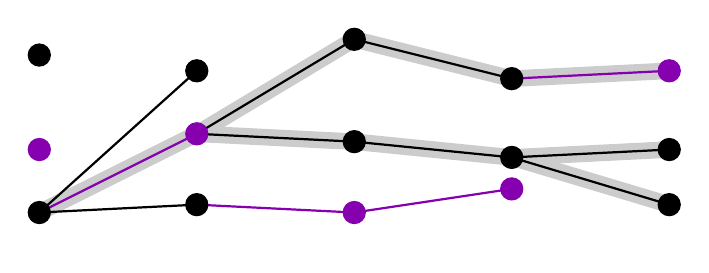
\begin{tikzpicture}
% highlight lineage 1
\draw[line width=6pt, gray!40] (0,0)--(2,1);
\draw[line width=6pt, gray!40] (2,1)--(4,2.2);
\draw[line width=6pt, gray!40] (4,2.2)--(6,1.7);
\draw[line width=6pt, gray!40] (6,1.7)--(8,1.8);
% highlight lineage 2
\draw[line width=6pt, gray!40] (2,1)--(4,0.9);
\draw[line width=6pt, gray!40] (4,0.9)--(6,0.7);
\draw[line width=6pt, gray!40] (6,0.7)--(8,0.8);
% highlight lineage 3
\draw[line width=6pt, gray!40] (6,0.7)--(8,0.1);
%
% lines column 1-2
\draw[thick] (0,0)--(2,0.1);
\draw[thick, violet] (0,0)--(2,1);
\draw[thick] (0,0)--(2,1.8);
% lines column 2-3
\draw[thick, violet] (2,0.1)--(4,0);
\draw[thick] (2,1)--(4,0.9);
\draw[thick] (2,1)--(4,2.2);
% lines column 3-4
\draw[thick, violet] (4,0)--(6,0.3);
\draw[thick] (4,0.9)--(6,0.7);
\draw[thick] (4,2.2)--(6,1.7);
% lines column 4-5
\draw[thick] (6,0.7)--(8,0.1);
\draw[thick] (6,0.7)--(8,0.8);
\draw[thick, violet] (6,1.7)--(8,1.8);
%
% nodes column 1
\filldraw (0,0) circle (4pt);
\filldraw[violet] (0,0.8) circle (4pt);
\filldraw (0,2) circle (4pt);
% nodes column 2
\filldraw (2,0.1) circle (4pt);
\filldraw[violet] (2,1) circle (4pt);
\filldraw (2,1.8) circle (4pt);
% nodes column 3
\filldraw[violet] (4,0) circle (4pt);
\filldraw (4,0.9) circle (4pt);
\filldraw (4,2.2) circle (4pt);
% nodes column 4
\filldraw[violet] (6,0.3) circle (4pt);
\filldraw (6,0.7) circle (4pt);
\filldraw (6,1.7) circle (4pt);
% nodes column 5
\filldraw (8,0.1) circle (4pt);
\filldraw (8,0.8) circle (4pt);
\filldraw[violet] (8,1.8) circle (4pt);
% fake line to add space
\draw[white] (0,-0.4)--(1,-0.4);
\end{tikzpicture}
\label{fig:whyASworks_b}
}
\caption[Why ancestor sampling works]{Illustration of how ancestor sampling prevents coalescence onto the immortal trajectory. Immortal particles are highlighted in purple, along with their parent-offspring edges (the given ones in \subref{fig:whyASworks_a} and the ancestor-sampled ones in \subref{fig:whyASworks_b}). The resulting lineages of the terminal particles are highlighted in grey. 
In \subref{fig:whyASworks_a}, the lineages of the terminal particles coalesce onto the immortal trajectory. Imagine time stretching further back: the lineages would continue to coincide with the immortal trajectory forever. 
In \subref{fig:whyASworks_b}, the lineages still coalesce, but not onto the immortal trajectory. The immortal trajectory no longer exists as a lineage.}
\label{fig:whyASworks}
\end{figure}



\chapter{Convergence of Finite-Dimensional Distributions} %\seb{$\checkmark$} }
\label{ch:limits}

%\epigraph{
%To see a World in a Grain of Sand\\
%And a Heaven in a Wild Flower,\\
%Hold Infinity in the palm of your hand\\
%And Eternity in an hour.
%}
%{\textsc{William Blake}} 

In this chapter we derive conditions under which genealogies induced by SMC algorithms converge to the $n$-coalescent as the number of particles tends to infinity. Here we prove only the convergence of finite-dimensional distributions; weak convergence is proved under the same conditions in Chapter~\ref{ch:weakconv}.

\section{Encoding genealogies}

\subsection{The genealogical process}
Before we can analyse genealogies, we need a way to encode them.
The encoding will only include the information relevant to the sample genealogy, namely which lineages coalesce at which times. Information about particle positions and ``killed'' particles is ignored.

Let $\mathcal{P}_n$ be the space of partitions on $\{1,\dots,n\}$.
For convenience, we now label time in reverse, so the terminal particles are at time 0, their parents are at time 1, and so on.
Consider a randomly chosen (uniformly, without replacement) sample of size $n$ among the $N$ terminal particles, and label the sampled particles $1,\dots,n$.
The genealogical process $(G_t^{(n,N)})_{t\in\mathbb{N}_0}$ for this sample is the $\mathcal{P}_n$-valued stochastic process such that labels $i$ and $j$ are in the same block of the partition $G_t^{(n,N)}$ if and only if terminal particles $i$ and $j$ have a common ancestor at time $t$ (i.e.\ $t$ generations back).

A formulation where $G_t^{(n,N)}$ takes values in the space of equivalence relations from $[n]$ to $[n]$ is sometimes used \parencite[e.g.][]{mohle1999}; interpreting partition blocks as equivalence classes, this formulation is equivalent to ours.

The initial value of the process is the partition of singletons $G_0^{(n,N)} = \{ \{1\}, \dots, \{n\} \}$, since all of the terminal particles are in separate lineages.
The only possible non-identity transitions are those that merge some blocks of the partition, encoding the coalescence of the corresponding lineages.
The trivial partition $\{ \{1,\dots,n\} \}$ is therefore an absorbing state, corresponding to all lineages in the sample having coalesced (i.e.\ the MRCA has been reached).
The construction of the genealogical process from the resampling relationships (i.e.\ the vector of parental indices at each generation) is illustrated in Figure \ref{fig:encoding_genealogy}.

\begin{figure}[ht]
\centering
\subfloat[Resampling relationships]{
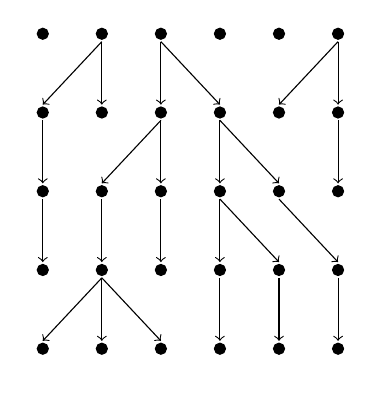
\begin{tikzpicture}
% grid of particles
\filldraw (0,0) circle (2pt);
\filldraw (0.75,0) circle (2pt);
\filldraw (1.5,0) circle (2pt);
\filldraw (2.25,0) circle (2pt);
\filldraw (3,0) circle (2pt);
\filldraw (3.75,0) circle (2pt);
\filldraw (0,1) circle (2pt);
\filldraw (0.75,1) circle (2pt);
\filldraw (1.5,1) circle (2pt);
\filldraw (2.25,1) circle (2pt);
\filldraw (3,1) circle (2pt);
\filldraw (3.75,1) circle (2pt);
\filldraw (0,2) circle (2pt);
\filldraw (0.75,2) circle (2pt);
\filldraw (1.5,2) circle (2pt);
\filldraw (2.25,2) circle (2pt);
\filldraw (3,2) circle (2pt);
\filldraw (3.75,2) circle (2pt);
\filldraw (0,3) circle (2pt);
\filldraw (0.75,3) circle (2pt);
\filldraw (1.5,3) circle (2pt);
\filldraw (2.25,3) circle (2pt);
\filldraw (3,3) circle (2pt);
\filldraw (3.75,3) circle (2pt);
\filldraw (0,4) circle (2pt);
\filldraw (0.75,4) circle (2pt);
\filldraw (1.5,4) circle (2pt);
\filldraw (2.25,4) circle (2pt);
\filldraw (3,4) circle (2pt);
\filldraw (3.75,4) circle (2pt);
% resampling arrows % generation 4 to 5
\draw[->] (0.75,0.9)--(0,0.1);
\draw[->] (0.75,0.9)--(0.75,0.1);
\draw[->] (0.75,0.9)--(1.5,0.1);
\draw[->] (2.25,0.9)--(2.25,0.1);
\draw[->] (3,0.9)--(3,0.1);
\draw[->] (3.75,0.9)--(3.75,0.1);
% resampling arrows % generation 3 to 4
\draw[->] (0,1.9)--(0,1.1);
\draw[->] (0.75,1.9)--(0.75,1.1);
\draw[->] (1.5,1.9)--(1.5,1.1);
\draw[->] (2.25,1.9)--(2.25,1.1);
\draw[->] (2.25,1.9)--(3,1.1);
\draw[->] (3,1.9)--(3.75,1.1);
% resampling arrows % generation 2 to 3
\draw[->] (0,2.9)--(0,2.1);
\draw[->] (1.5,2.9)--(0.75,2.1);
\draw[->] (1.5,2.9)--(1.5,2.1);
\draw[->] (2.25,2.9)--(2.25,2.1);
\draw[->] (2.25,2.9)--(3,2.1);
\draw[->] (3.75,2.9)--(3.75,2.1);
% resampling arrows % generation 1 to 2
\draw[->] (0.75,3.9)--(0,3.1);
\draw[->] (0.75,3.9)--(0.75,3.1);
\draw[->] (1.5,3.9)--(1.5,3.1);
\draw[->] (1.5,3.9)--(2.25,3.1);
\draw[->] (3.75,3.9)--(3,3.1);
\draw[->] (3.75,3.9)--(3.75,3.1);
% fudge bottom space
\node[anchor=north] at (0,0) {\textcolor{white}{\footnotesize{1}}};
\end{tikzpicture}
\label{fig:encoding_a}
}
\hspace{0.6cm}
\subfloat[Genealogy of terminal particles]{
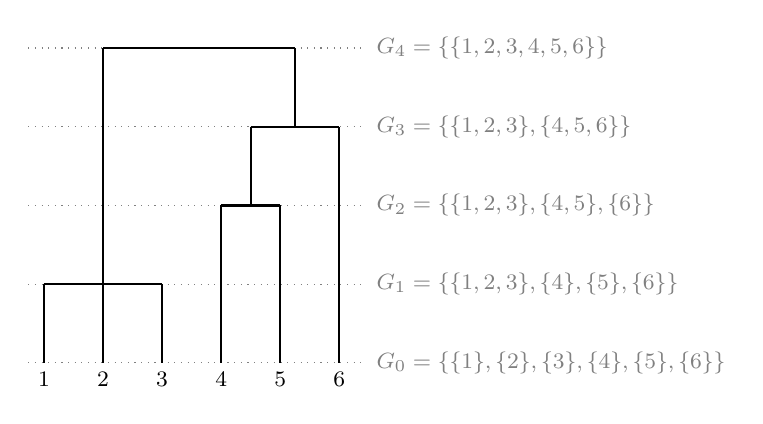
\begin{tikzpicture}
% horizontal time lines
\draw[gray,dotted] (-0.2,0)--(4.05,0);
\draw[gray,dotted] (-0.2,1)--(4.05,1);
\draw[gray,dotted] (-0.2,2)--(4.05,2);
\draw[gray,dotted] (-0.2,3)--(4.05,3);
\draw[gray,dotted] (-0.2,4)--(4.05,4);
% tree
\draw[thick] (0.75,0)--(0.75,4);
\draw[thick] (0,0)--(0,1);
\draw[thick] (1.5,0)--(1.5,1);
\draw[thick] (0,1)--(1.5,1);
\draw[thick] (2.25,0)--(2.25,2);
\draw[thick] (3,0)--(3,2);
\draw[thick] (2.25,2)--(3,2);
\draw[thick] (2.625,2)--(2.625,3);
\draw[thick] (3.75,0)--(3.75,3);
\draw[thick] (2.625,3)--(3.75,3);
\draw[thick] (3.1875,3)--(3.1875,4);
\draw[thick] (0.75,4)--(3.1875,4);
% lineage labels
\node[anchor=north] at (0,0) {\footnotesize{1}};
\node[anchor=north] at (0.75,0) {\footnotesize{2}};
\node[anchor=north] at (1.5,0) {\footnotesize{3}};
\node[anchor=north] at (2.25,0) {\footnotesize{4}};
\node[anchor=north] at (3,0) {\footnotesize{5}};
\node[anchor=north] at (3.75,0) {\footnotesize{6}};
% partition labels
\node[anchor=west] at (4.1,0) {\textcolor{gray}{\footnotesize{$G_0 = \{ \{1\}, \{2\}, \{3\}, \{4\}, \{5\}, \{6\} \}$}}};
\node[anchor=west] at (4.1,1) {\textcolor{gray}{\footnotesize{$G_1 = \{ \{1,2,3\}, \{4\}, \{5\}, \{6\} \}$}}};
\node[anchor=west] at (4.1,2) {\textcolor{gray}{\footnotesize{$G_2 = \{ \{1,2,3\}, \{4,5\}, \{6\} \}$}}};
\node[anchor=west] at (4.1,3) {\textcolor{gray}{\footnotesize{$G_3 = \{ \{1,2,3\}, \{4,5,6\} \}$}}};
\node[anchor=west] at (4.1,4) {\textcolor{gray}{\footnotesize{$G_4 = \{ \{1,2,3,4,5,6\} \}$}}};
\end{tikzpicture}
\label{fig:encoding_b}
}
\caption[Encoding the sample genealogy]{Illustration of how the sample genealogy is encoded. 
\subref{fig:encoding_a} Relationships induced by resampling in a sample of $n=6$ particles over four iterations. For clarity the pictured example has $n=N$, but in general $n \ll N$. 
\subref{fig:encoding_b} The genealogy of these six particles, labelled with the value of the genealogical process $G_t$ at each time.}
\label{fig:encoding_genealogy}
\end{figure}

Under the assumption \ref{standing_assumption} stated below, it is sufficient for our purposes to consider only offspring counts $\nu_t^{(1:N)} = (\nu_t^{(1)},\dots,\nu_t^{(N)})$, where $\nu_t^{(i)} = |\{ j: a_t^{(j)} =i \}|$, rather than the parental indices $a_t^{(1:N)}$ which are generally more informative.
\begin{enumerate}[label=(A\arabic*)]
\item\label{standing_assumption} The conditional distribution of parental indices $a_t^{(1:N)}$ given offspring counts $\nu_t^{(1:N)}$ is uniform over all assignments such that $ |\{ j: a_t^{(j)} =i \}|= \nu_t^{(i)} $ for all $i$.
%valid assignments.
\end{enumerate}
As we saw in Section~\ref{sec:coaltheory}, the $n$-coalescent is \emph{exchangeable}, so for instance the pair of lineages merging at each event is chosen uniformly. 
\ref{standing_assumption} is a weaker condition than exchangeability of the particles within a generation which is sufficient to admit an exchangeable process in the limit.
Although the resampling in SMC is not generally exchangeable, %(conditional on previous iterations/weights, anyway --- if completely unconditioned then I guess the distn is exchangeable, but I don't think that's what's meant in pop gen either.)
\ref{standing_assumption} can easily be enforced upon any SMC algorithm by applying a random permutation to the offspring indices immediately after resampling.
%, without qualitatively affecting the dynamics.




\subsection{Time scale}
In order to have a well-defined limit for the genealogical process as $N\to\infty$, we must scale time by a suitable function $\tau_N(\cdot)$. In the population genetics literature the time scale function is typically deterministic (Section~\ref{sec:popgenmodels}), but in our case $\tau_N$ depends on the offspring counts and is therefore random.
To define the time scale we first define the pair merger rate
\begin{equation}\label{eq:defn_cN}
c_N(t) := \frac{1}{(N)_2} \sum_{i=1}^N (\nu_t^{(i)})_2 .
\end{equation}
This is the probability, conditional on $\nu_t^{(1:N)}$, that a randomly chosen pair of lineages in generation $t$ merges exactly one generation back.
The given expression for $c_N(t)$ is justified by assumption \ref{standing_assumption},  as are the expressions for $\tau_N(t)$ and $D_N(t)$ below.
To achieve a limiting pair merger rate of 1, as in the $n$-coalescent, we rescale time by the generalised inverse
\begin{equation}\label{eq:defn_tauN}
\tau_N(t) := \inf \left\{ s \in \mathbb{N} : \sum_{r=1}^s c_N(r) \geq t \right\} .
\end{equation}
The function $\tau_N$ maps continuous to discrete time, providing the link between the discrete-time SMC dynamics and the continuous-time limit.
We will also need the following quantity, which is an upper bound on the conditional probability of a multiple merger (three or more lineages merging, or two or more simultaneous pairwise mergers):
\begin{equation}\label{eq:defn_DN}
D_N(t) := \frac{1}{N(N)_2} \sum_{i=1}^N (\nu_t^{(i)})_2
        \left\{ \nu_t^{(i)} + \frac{1}{N} \sum_{j\neq i} (\nu_t^{(j)})^2 \right\} .
\end{equation} 
This will be used to control the rate of multiple mergers, which must be dominated by the pair-merger rate as $N\to\infty$ if we are to recover a Kingman limit (in which almost surely the only non-identity transitions are pair mergers).
%Let $\nu_t^{(i)}$ be the number of offspring in generation $t$ of particle $i$ ($t \in \mathbb{N}$, $i = 1,\dots, N$).
%Let $(\mathcal{F}_t)$ be the reverse-time filtration generated by the offspring counts.
Some basic properties of $c_N$, $D_N$ and $\tau_N$ are stated in Proposition~\ref{thm:cN_properties}.
\begin{prop}\label{thm:cN_properties}
For all $t\in\mathbb{N}$, $t^\prime > s^\prime >0$,
\begin{enumerate}[label=(\alph*)]
\item \label{item:cN_property1} \hspace{5pt}
    $\begin{aligned}
    c_N(t) , D_N(t) \in [0,1]
    \end{aligned}$
\item \label{item:cN_property2} \hspace{5pt}
    $\begin{aligned}
    D_N(t) \leq c_N(t)
    \end{aligned}$
\item \label{item:cN_property3} \hspace{5pt}
    $\begin{aligned}
    c_N(t)^2 \leq c_N(t) 
    \end{aligned}$
\item \label{item:cN_property4} \hspace{5pt}
    $\begin{aligned}
    t^\prime
    \leq \sum_{r=1}^{\tau_N(t^\prime)} c_N(r) 
    \leq t^\prime +1 .
    \end{aligned}$
\item \label{item:cN_property5} \hspace{5pt}
    $\begin{aligned}
    t^\prime - s^\prime -1
    \leq \sum_{r=\tau_N(s^\prime)+1}^{\tau_N(t^\prime)} c_N(r) 
    \leq t^\prime - s^\prime +1 .
    \end{aligned}$
\item \label{item:cN_property6} \hspace{5pt}
    $\begin{aligned}
    \tau_N(t^\prime) \geq t^\prime .
    \end{aligned}$
\end{enumerate}
%\begin{align}
%& c_N(t) , D_N(t) \in [0,1] \label{eq:cN_property1}\\
%& D_N(t) \leq c_N(t) \label{eq:cN_property2}\\
%& c_N(t)^2 \leq c_N(t) \label{eq:cN_property3}\\
%& t^\prime \leq \sum_{r=1}^{\tau_N(t^\prime)} c_N(r) \leq t^\prime +1 . \label{eq:cN_property4}
%\end{align}
\end{prop}

\begin{proof}
\textbf{\ref{item:cN_property1}}  $c_N(t)$ and $D_N(t)$ are clearly non-negative. Both are maximised when one of the offspring counts is equal to $N$ and the rest are zero, in which case $c_N(t) = D_N(t) = 1$.\\
\textbf{\ref{item:cN_property2}} As outlined in \textcite[p.9]{koskela2018},
\begin{align*}
D_N(t) &:= \frac{1}{(N)_2} \sum_{i=1}^N (\nu_t^{(i)})_2 \frac{1}{N} \left\{  \nu_t^{(i)} + \frac{1}{N} \sum_{j\neq i}^N (\nu_t^{(j)})^2 \right\} \\
&\leq \frac{1}{(N)_2} \sum_{i=1}^N (\nu_t^{(i)})_2 \frac{1}{N} \left\{  \nu_t^{(i)} + \frac{1}{N} \sum_{j\neq i}^N N \nu_t^{(j)} \right\} \\
&= \frac{1}{(N)_2} \sum_{i=1}^N (\nu_t^{(i)})_2 \frac{1}{N} \left\{ \sum_{j =1}^N \nu_t^{(j)} \right\}
= \frac{1}{(N)_2} \sum_{i=1}^N (\nu_t^{(i)})_2
= c_N(t) .
\end{align*}
\textbf{\ref{item:cN_property3}} is immediate given \ref{item:cN_property1}.\\
\textbf{\ref{item:cN_property4}} follows directly from the definition of $\tau_N$ in \eqref{eq:defn_tauN}.\\
\textbf{\ref{item:cN_property5}} Writing
\begin{equation*}
\sum_{r=\tau_N(s^\prime)+1}^{\tau_N(t^\prime)} c_N(r)
= \sum_{r=1}^{\tau_N(t^\prime)} c_N(r) 
        - \sum_{r=1}^{\tau_N(s^\prime)} c_N(r) ,
\end{equation*}
the result follows by applying \ref{item:cN_property4} to both sums.\\
\textbf{\ref{item:cN_property6}} follows from \ref{item:cN_property1} and the definition of $\tau_N$ in \eqref{eq:defn_tauN}.
\end{proof}


Another useful property is the following, based on \textcite[Lemma 2]{koskela2018}. There the special case $f(r) \equiv c_N(r)$ is proved, but the authors remark that the result also holds for other choices of $f$. Here we state the result in full generality.

\begin{lemma}\label{thm:kjjslemma2}
Fix $t>0$.
Let $(\mathcal{F}_r)$ be the backwards-in-time filtration generated by the offspring counts $\nu_r^{(1:N)}$ at each generation $r$.
Let $f$ be any deterministic function of $\nu_r^{(1:N)}$ such that for all $\nu^{(1:N)}$ there exists $B<\infty$ for which $0\leq f(\nu^{(1:N)}) \leq B$.
Then
\begin{equation*}
\E \left[ \sum_{r=1}^{\tau_N(t)} f(\nu_r^{(1:N)}) \right] 
= \E \left[ \sum_{r=1}^{\tau_N(t)} \E [ f(\nu_r^{(1:N)}) \mid \mathcal{F}_{r-1} ] \right] .
\end{equation*}
\end{lemma}
The lemma holds more generally for any bounded function $f$ (i.e.\ that does not need to be non-negative) by decomposing into the positive and negative parts. However, the simplified statement here is sufficient for our purposes since we will only apply the lemma to non-negative functions.

\begin{proof}
Define 
\begin{equation*}
M_s 
:= \sum_{r=1}^s \left\{ f(\nu_r^{(1:N)}) 
        - \E [ f(\nu_r^{(1:N)}) \mid \mathcal{F}_{r-1} ] \right\} .
\end{equation*}
It is easy to establish that $(M_s)$ is a martingale with respect to $(\mathcal{F}_s)$, and $M_0 = 0$. 
Now fix $K\geq 1$ and note that $\tau_N(t) \wedge K$ is a bounded $\mathcal{F}_t$-stopping time.
Hence we can apply the optional stopping theorem:
\begin{align*}
\E [M_{\tau_N(t) \wedge K} ]
&= \E \left[ \sum_{r=1}^{\tau_N(t) \wedge K} \left\{ f(\nu_r^{(1:N)}) 
        - \E [ f(\nu_r^{(1:N)}) \mid \mathcal{F}_{r-1} ] \right\} \right] \\
&= \E \left[ \sum_{r=1}^{\tau_N(t) \wedge K} f(\nu_r^{(1:N)}) \right]
        - \E \left[ \sum_{r=1}^{\tau_N(t) \wedge K} 
        \E [ f(\nu_r^{(1:N)}) \mid \mathcal{F}_{r-1} ] \right]
=0 .
\end{align*}
Since this holds for all $K\geq 1$,
\begin{equation*}
\lim_{K\to\infty} \E \left[ \sum_{r=1}^{\tau_N(t) \wedge K} f(\nu_r^{(1:N)}) \right]
= \lim_{K\to\infty} \E \left[ \sum_{r=1}^{\tau_N(t) \wedge K} 
        \E [ f(\nu_r^{(1:N)}) \mid \mathcal{F}_{r-1} ] \right] .
\end{equation*}
The monotone convergence theorem allows the limit to pass inside the expectation on each side (since increasing $K$ can only increase each sum, by possibly adding some non-negative terms). Hence
\begin{align*}
\E \left[ \sum_{r=1}^{\tau_N(t)} f(\nu_r^{(1:N)}) \right]
&= \E \left[ \lim_{K\to\infty} \sum_{r=1}^{\tau_N(t) \wedge K} f(\nu_r^{(1:N)}) \right]
= \E \left[ \lim_{K\to\infty} \sum_{r=1}^{\tau_N(t) \wedge K} 
        \E [ f(\nu_r^{(1:N)}) \mid \mathcal{F}_{r-1} ] \right] \\
&= \E \left[ \sum_{r=1}^{\tau_N(t)} 
        \E [ f(\nu_r^{(1:N)}) \mid \mathcal{F}_{r-1} ] \right] ,
\end{align*}
which concludes the proof.
\end{proof}



\subsection{Transition probabilities}
%Let $\mathcal{P}_n$ be the space of partitions of $\{1,\dots,n\}$, and denote by $\Delta$ the partition of singletons $\{ \{1\},\dots, \{n\} \}$.
Recall that $\mathcal{P}_n$ denotes the space of partitions of $\{1,\dots,n\}$.
For any $\xi, \eta \in \mathcal{P}_n$ and $t\in\mathbb{N}$, let $p_{\xi\eta}(t)$ denote the conditional transition probabilities of the genealogical process given $\nu_t^{(1:N)}$. % ($t\in\mathbb{N}$, $\xi, \eta \in \mathcal{P}_n$).
The transition probability $p_{\xi\eta}(t)$ can only be non-zero when $\eta$ is obtained from $\xi$ by merging some blocks of $\xi$ (i.e.\ some lineages coalescing).
Ordering the blocks by their least element, denote by $b_i$ the number of blocks of $\xi$ that merge to form block $i$ in $\eta$, for each $i \in \{1,\dots, |\eta|\}$. Hence $b_1 + \cdots + b_{|\eta|} = |\xi|$.
Then the transition probability is given by
\begin{equation}\label{eq:defn_pxieta}
p_{\xi\eta}(t) 
:= \frac{1}{(N)_{|\xi|}} \sum_{\substack{i_1 , \ldots , i_{|\eta|} =1 
        \\ \text{all distinct} }}^N
        (\nu_t^{(i_1)})_{b_1} \cdots (\nu_t^{(i_{|\eta|})})_{b_{|\eta|}} .
\end{equation}
This expression is justified by \ref{standing_assumption}.
We will only need to work directly with the identity transition probabilities $p_{\xi\xi}(t)$.
Upper and lower bounds on these probabilities are presented in Propositions \ref{thm:pDelta_LB} and \ref{thm:pDelta_UB}.
\begin{prop}%[Lower bound on identity transition probabilities]
\label{thm:pDelta_LB}
Let $\xi \in \mathcal{P}_n$, $N>2$. Then
\begin{equation*}
p_{\xi\xi}(t)
\geq 1 - \binom{|\xi|}{2} \frac{N^{|\xi|-2}}{(N-2)_{|\xi|-2}} \left[ c_N(t) + B_{|\xi|} D_N(t) \right]
\end{equation*}
where 
\begin{equation*}
B_{|\xi|} = K (|\xi|-1)! (|\xi|-2) \exp( 2 \sqrt{2(|\xi|-2)} )
\end{equation*}
for some $K>0$ that does not depend on $|\xi|$.
\end{prop}
%\seb{For weak convergence proof, refer to this proposition but rewrite the inequality using $\xi = \Delta$ and $\alpha_n$, to provide a local target for cross-referencing. Similarly for UB.}
\begin{proof}
%The proof follows \textcite[Proof of Lemma 3.6]{brown2021}, but keeping the terms in $N$ explicit. --- I don't need to refer to BJJK as it's part of my work; just reproduce BJJK's workings nice and verbosely here :)
We have the following expression for $p_{\xi\xi}(t)$, by subtracting all possible non-identity transitions. The sum over $k$ counts all transitions from $\xi$ to $\eta$ such that $k= |\eta| \leq |\xi|-1$; the omitted $k=|\xi|$ term would count identity transitions.
\begin{equation*}
p_{ \xi \xi }( t ) 
= 1 - \frac{ 1 }{ ( N )_{ | \xi | } } \sum_{ k = 1 }^{ | \xi | - 1 } 
        \sum_{ \substack{ b_1 \geq \ldots \geq b_k \geq 1 
        \\ b_1 + \ldots + b_k = | \xi | } } 
        \frac{ | \xi |! }{ \prod_{ j = 1 }^{ | \xi | } ( j ! )^{ \kappa_j } \kappa_j ! } 
        \sum_{ \substack{ i_1, \ldots, i_k = 1 \\ \text{all distinct} } }^N 
        ( \nu_t^{ ( i_1 ) } )_{ b_1 } \ldots ( \nu_t^{ ( i_k ) } )_{ b_k },
\end{equation*}
where $\kappa_i = |\{ j : b_j = i \}|$ is the multiplicity of mergers of size $i$ ($\kappa_1$ counts non-merger events, and we have the identity $\kappa_1 + 2 \kappa_2 + \cdots + | \xi | \kappa_{ | \xi | } = | \xi |$).
The combinatorial factor is the number of partitions of a sequence of length $|\xi|$  having $\kappa_j$ subsequences of length $j$ for each $j$ \parencite[Equation (11)]{fu2006}.
%Throughout this document, where no lower summation limit is specified, each sum index ranges from 1 to the upper limit, under any specified constraints.

We separate the $k=|\xi|-1$ term (which counts single pair mergers), for which\\ $(b_1, b_2, \dots, b_{|\xi|-1}) = (2,1,\dots,1)$ and
\begin{equation*}
\frac{ | \xi |! }{ \prod_{ j = 1 }^{ | \xi | } ( j ! )^{ \kappa_j } \kappa_j ! }
= \binom{|\xi|}{2} .
\end{equation*}
For the remaining terms we use
\begin{equation*}
\frac{ | \xi |! }{ \prod_{ j = 1 }^{ | \xi | } ( j ! )^{ \kappa_j } \kappa_j ! }
\leq |\xi|! .
\end{equation*}
Thus
\begin{align}
p_{ \xi \xi }( t ) 
&\geq 1 - \frac{ 1 }{ ( N )_{ | \xi | } } \binom{|\xi|}{2}
        \sum_{ \substack{ i_1, \ldots, i_{|\xi|-1} = 1 \\ \text{all distinct} } }^N 
        ( \nu_t^{ ( i_1 ) } )_2 \nu_t^{(i_2)} \ldots \nu_t^{ ( i_{|\xi|-1} ) } \notag\\
    &\qquad- \frac{ 1 }{ ( N )_{ | \xi | } } \sum_{ k = 1 }^{ | \xi | - 2 } 
        \sum_{ \substack{ b_1 \geq \ldots \geq b_k \geq 1 
        \\ b_1 + \ldots + b_k = | \xi | } } |\xi|!
        \sum_{ \substack{ i_1, \ldots, i_k = 1 \\ \text{all distinct} } }^N 
        ( \nu_t^{ ( i_1 ) } )_{ b_1 } \ldots ( \nu_t^{ ( i_k ) } )_{ b_k } \label{eq:pDeltaLB_1}
\end{align}
Now, for the $k=|\xi|-1$ term we use the bound
\begin{equation*}
\sum_{\substack{ i_1, \ldots, i_{ | \xi | - 1 } = 1 \\ \text{all distinct} }}^N 
        ( \nu_t^{ ( i_1 ) } )_2 \nu_t^{ ( i_2 ) } \ldots \nu_t^{ ( i_{ | \xi | - 1 } ) }
\leq N^{ | \xi | - 2 } \sum_{ i = 1 }^N ( \nu_t^{ ( i ) } )_2
\end{equation*}
while for the other terms we have \parencite[similarly to][Lemma 1 Case 3]{koskela2018}
\begin{align*}
\sum_{ \substack{ i_1, \ldots, i_k = 1 \\ \text{all distinct} } }^N 
        &( \nu_t^{ ( i_1 ) } )_{ b_1 } \ldots ( \nu_t^{ ( i_k ) } )_{ b_k } \\
&\leq \sum_{ i = 1 }^N ( \nu_t^{ ( i ) } )_2 
        \Bigg\{ \sum_{\substack{ j_1, \ldots, j_{ | \xi | - 2 } = 1 }}^N
        \nu_t^{ ( j_1 ) } \ldots \nu_t^{ ( j_{ | \xi | - 2 } ) }
        - \sum_{ \substack{ j_1, \ldots, j_{ | \xi | - 2 } = 1 
        \\ \text{all distinct and } \neq i } }^N 
        \nu_t^{ ( j_1 ) } \ldots \nu_t^{ ( j_{ | \xi | - 2 } ) } \Bigg\} \\
&= \sum_{ i = 1 }^N ( \nu_t^{ ( i ) } )_2 
        \Bigg\{ \Bigg( \sum_{j=1}^N \nu_t^{(j)} \Bigg)^{|\xi|-2}
        - \sum_{ \substack{ j_1, \ldots, j_{ | \xi | - 2 } = 1 
        \\ \text{all distinct and } \neq i } }^N 
        \nu_t^{ ( j_1 ) } \ldots \nu_t^{ ( j_{ | \xi | - 2 } ) } \Bigg\} 
\end{align*}
where we have subtracted all the terms except those which either have one of the indices equal to $i$ (in which case the largest merger consists of more than two lineages) or have two of the indices equal to each other (in which case there is a simultaneous merger).
This leaves only those terms where $k\leq |\xi|-2$, that is where there are multiple or simultaneous mergers. It is an inequality rather than an equality because some of the cases are double-counted.

The expression is further bounded by a reverse multinomial expansion, of the same form as \textcite[Equation (8)]{koskela2018}, which is then simplified using that $(N - x)^b \geq N^b - b x N^{ b - 1 }$ 
for $x \leq N$, $b \geq 0$, an application of the Bernoulli inequality:
\begin{align*}
& \sum_{ i = 1 }^N ( \nu_t^{ ( i ) } )_2 
        \Bigg\{ N^{ | \xi | - 2 } - ( N - \nu_t^{ ( i ) } )^{ | \xi | - 2 } 
        + \binom{ | \xi | - 2 }{ 2 } \sum_{ j \neq i } ( \nu_t^{ ( j ) } )^2 
        \Bigg( \sum_{ k \neq i } \nu_t^{ ( k ) } \Bigg)^{ | \xi | - 4 } \Bigg\} \\
&\leq \sum_{ i = 1 }^N ( \nu_t^{ ( i ) } )_2 
        \Bigg\{ ( | \xi | - 2 ) \nu_t^{ ( i ) } N^{ | \xi | - 3 } 
        + \binom{ | \xi | - 2 }{ 2 } \sum_{ j \neq i } ( \nu_t^{ ( j ) } )^2 N^{ | \xi | - 4 } 
        \Bigg\} ,
\end{align*}
%where the last step uses $(N - x)^b \geq N^b - b x N^{ b - 1 }$ 
%for $x \leq N$, $b \geq 0$, which is an application of the Bernoulli inequality.
Hence
\begin{align*}
p_{ \xi \xi }( t ) 
&\geq 1 - \frac{ 1 }{ ( N )_{ | \xi | } } \binom{|\xi|}{2}
        N^{ | \xi | - 2 } \sum_{ i = 1 }^N ( \nu_t^{ ( i ) } )_2 \\
    &\qquad- \frac{ N^{|\xi|-3} }{ ( N )_{ | \xi | } } |\xi|!
        \sum_{ k = 1 }^{ | \xi | - 2 } 
        \sum_{ \substack{ b_1 \geq \ldots \geq b_k \geq 1 
        \\ b_1 + \ldots + b_k = | \xi | } } 
        \sum_{ i = 1 }^N ( \nu_t^{ ( i ) } )_2 
        \Bigg\{ ( | \xi | - 2 ) \nu_t^{ ( i ) } + \binom{ | \xi | - 2 }{ 2 } \frac{1}{N} 
        \sum_{ j \neq i } ( \nu_t^{ ( j ) } )^2 \Bigg\} .
\end{align*}
The summands in the last line are independent of $k, b_1, \dots, b_k$, and the number of terms in the sums over $k$ and $b_1, \dots, b_k$ is bounded by $\gamma_{|\xi|-2} (|\xi|-2)$, where $\gamma_n$ is the number of integer partitions of $n$.
By \textcite[Section 2]{hardy1918}, $\gamma_n < K e^{ 2 \sqrt{ 2 n } } / n$ for a constant $K > 0$ independent of $n$.
Thus, for $|\xi| > 2$,
\begin{align*}
p_{ \xi \xi }( t ) 
&\geq 1 - \frac{ N^{ | \xi | - 2 } }{ ( N-2 )_{ | \xi | -2} } \binom{|\xi|}{2}
        c_N(t) \\
    &\qquad- \frac{ N^{|\xi|-2} }{ ( N-2 )_{ | \xi | -2} }
        K \exp( 2 \sqrt{2(|\xi|-2)} ) |\xi|!
        \frac{1}{N(N)_2} \\
    &\hspace{4cm}\times \sum_{ i = 1 }^N ( \nu_t^{ ( i ) } )_2
        \Bigg\{ ( | \xi | - 2 ) \nu_t^{ ( i ) } + \binom{ | \xi | - 2 }{ 2 } \frac{1}{N} 
        \sum_{ j \neq i } ( \nu_t^{ ( j ) } )^2 \Bigg\} .
\end{align*}
Notice that when $|\xi| > 2$, both $(|\xi|-2)$ and $\binom{|\xi|-2}{2}$ are less than or equal to $\binom{|\xi|-1}{2}$. Thus by definition of $D_N(t)$,
\begin{align*}
p_{ \xi \xi }( t ) 
&\geq 1 - \frac{ N^{ | \xi | - 2 } }{ ( N-2 )_{ | \xi | -2} } \binom{|\xi|}{2}
        c_N(t) \\
    &\qquad- \frac{ N^{|\xi|-2} }{ ( N-2 )_{ | \xi | -2} }
        K \exp( 2 \sqrt{2(|\xi|-2)} ) |\xi|! \binom{ |\xi|-1}{2} D_N(t) \\
&\geq 1 - \frac{ N^{ | \xi | - 2 } }{ ( N-2 )_{ | \xi | -2} } \binom{|\xi|}{2}
        \left[ c_N(t) + B_{|\xi|} D_N(t) \right]
\end{align*}
where
\begin{align*}
B_{|\xi|} 
&= \binom{|\xi|}{2}^{-1} K \exp( 2 \sqrt{2(|\xi|-2)} ) |\xi|! \binom{ |\xi|-1}{2} \\
&= K (|\xi|-1)! (|\xi|-2) \exp( 2 \sqrt{2(|\xi|-2)} ) .
\end{align*}
%When $|\xi| \leq 2$, there are no terms with $k\leq |\xi|-2$, and the result is immediate.
When $|\xi| = 2$, \eqref{eq:pDeltaLB_1} becomes 
\begin{equation*}
p_{ \xi \xi }( t )
\geq 1 - c_N(t)
\end{equation*}
and when $|\xi| = 1$, 
\eqref{eq:pDeltaLB_1} becomes 
\begin{equation*}
p_{ \xi \xi }( t )
\geq 1 ;
\end{equation*}
in both cases the result is immediate.
\end{proof}


\begin{prop}%[Upper bound on identity transition probabilities]
\label{thm:pDelta_UB}
Let $\xi \in \mathcal{P}_n$. Then, for $N$ sufficiently large,
\begin{equation*}
p_{\xi\xi}(t)
\leq 1 - \binom{|\xi|}{2} \{ 1 + O(N^{-1}) \} 
        \left[ c_N(t) - B_{|\xi|}^\prime D_N(t) \right]
\end{equation*}
where $B_{|\xi|}^\prime = \binom{|\xi|-1}{2}$.
\end{prop}

A proof is given in \textcite[Lemma 1 Case 1]{koskela2018}.\seb{refer to the erratum once available, which is more explicit about this proof.}





\section{An existing limit theorem}
\textcite{koskela2018} proved the following theorem which gives sufficient conditions under which sampled genealogies of (non-neutral) interacting particle systems converge to the $n$-coalescent as $N\to\infty$.
Such a result can only be expected to hold for genealogies of finite samples ($n\ll N$), and not for the entire genealogy of the $N$ particles. 
For instance the genealogies arising in SMC algorithms are not restricted to single pair mergers only, although within a sparse sample we may, under mild conditions, see only single pair mergers. 
That is to say, there is not an extension of this result whereby the whole-population genealogy converges to the Kingman coalescent as $N\to\infty$, unless very restrictive conditions are imposed.

\begin{theorem}[\cite{koskela2018}]\label{thm:kjjs_mainthm}
Fix $n \leq N$ as the observed number of particles from the output of an interacting particle system with $N$ particles which satisfies \ref{standing_assumption}.
Suppose that for any $0 \leq s < t < \infty$, we have
\begin{gather}\label{eq:kjjs_big_merger_bound}
\lim_{ N \rightarrow \infty } \E\Bigg[ \sum_{ r = \tau_N( s ) + 1 }^{ \tau_N( t ) } D_N( r ) \Bigg] = 0, \\
%\end{equation}
%\begin{equation}
\label{eq:kjjs_binary_bound}
\lim_{ N \rightarrow \infty } \E[ c_N( t ) ] = 0, \\
%\end{equation}
%\begin{equation}
\label{eq:kjjs_binary_bound_2}
\lim_{ N \rightarrow \infty } \E\Bigg[ \sum_{ r = \tau_N( s ) + 1 }^{ \tau_N( t ) } c_N( r )^2 \Bigg] = 0, \\
%\end{equation}
%and
%\begin{equation}
\label{eq:kjjs_tau_bound}
\text{and}\qquad\qquad\E[ \tau_N( t ) - \tau_N( s ) ] \leq C_{ t, s } N,\qquad\qquad\phantom{\text{and}}
\end{gather}
for some constant $C_{ t, s } > 0$ that is independent of $N$.
Then $( G_{ \tau_N( t ) }^{ ( n, N ) } )_{ t \geq 0 }$ converges to the Kingman $n$-coalescent in the sense of finite-dimensional distributions as $N \rightarrow \infty$. 
\end{theorem}

To ensure samples of size $n$ have Kingman genealogies in the limit, with pair mergers only, we require that multiple mergers (that is, where more than two lineages merge into one, or where two or more mergers happen simultaneously) occur on a slower time scale than pair mergers. 
This is the role of condition \eqref{eq:kjjs_big_merger_bound}.

Conditions \eqref{eq:kjjs_binary_bound} and \eqref{eq:kjjs_binary_bound_2} ensure that the limiting process is continuous and has the required unit pair merger rate.
%, and will not be violated by any reasonable SMC algorithm. 
For \eqref{eq:kjjs_binary_bound} to fail to hold, the expected number of mergers at some generation would have to be $\Omega(N^2)$. This can only happen if the resampling scheme is very bad (e.g.\ star resampling) or the weights are particularly badly-behaved. The latter is ruled out in the corollaries of Chapter~\ref{ch:appl} by imposing bounds on the potential functions; this is discussed further in Section~\ref{sec:corol_mn}.

Condition \eqref{eq:kjjs_tau_bound} specifies that the time scale must be $O(N)$. As we saw in Section~\ref{sec:popgenmodels}, this is the correct time scale for the Wright-Fisher model, but for instance the Moran model has time scale $O(N^2)$ and hence violates this condition. 
Since we know that the neutral Moran model also has Kingman genealogies in the limit, condition \eqref{eq:kjjs_tau_bound} clearly is not necessary. 
The simplified statement in Theorem~\ref{thm:FDDconv} does not impose any such condition on the time scale.

The proof of \textcite{koskela2018} does not explicitly use \eqref{eq:kjjs_binary_bound} but rather the similar condition
\begin{equation}\label{eq:kjjs_binary_bound_corrected}
\lim_{ N \rightarrow \infty } \E[ c_N( \tau_N(t) ) ] = 0 .
\end{equation}
However, as we will see in the next section (Lemmata \ref{thm:DNimpliescN} and \ref{thm:DNimpliescN_2}), both \eqref{eq:kjjs_binary_bound} and \eqref{eq:kjjs_binary_bound_corrected} are implied by \eqref{eq:kjjs_big_merger_bound}, so the theorem is correct. 
Such redundancies in the statement of Theorem~\ref{thm:kjjs_mainthm} are removed in Theorem~\ref{thm:FDDconv}.

%%%%

The proof of Theorem~\ref{thm:kjjs_mainthm} \parencite[i.e.][Theorem 1]{koskela2018} proceeds in three parts.
The first is a vanishing upper bound on finite-dimensional distributions of the genealogical process when the path of the process involves any multiple mergers.
%, either multiple simultaneous mergers or any merger involving more than two particles.
The second is showing that, when the path of the genealogy consists of only single pair mergers, the finite-dimensional distributions of the $n$-coalescent upper bound those of the genealogical process in the limit $N\to\infty$.
The final piece is a similar lower bound, which together with the upper bound establishes convergence of the finite-dimensional distributions.




\section{A new limit theorem}
We now present a related theorem, having the same conclusion but with conditions that are more tractable and remove some redundancies in the statement of Theorem~\ref{thm:kjjs_mainthm}. 
%While we do not prove that this is a strict generalisation, there are certainly systems which satisfy the conditions of Theorem~\ref{thm:FDDconv} but not of Theorem~\ref{thm:kjjs_mainthm}.

\begin{theorem}\label{thm:FDDconv}
Let $\nu_t^{(1:N)}$ denote the offspring numbers in an interacting particle system satisfying \ref{standing_assumption} such that, for any $N$ sufficiently large, $\Prob[ \tau_N(t) = \infty ] =0$ for all finite $t$. Suppose that there exists a deterministic sequence $(b_N)_{N\geq1}$ such that ${\lim}_{N\to\infty} b_N =0$ and
\begin{equation}\label{eq:mainthmcond}
\frac{1}{(N)_3} \sum_{i = 1}^N \Et[ (\nu_t^{(i)})_3 ]  \leq b_N \frac{1}{(N)_2} \sum_{i = 1}^N \Et[ (\nu_t^{(i)})_2 ]
\end{equation}
for all $N$, uniformly in $t \geq 1$.
Fix $n\leq N$ and consider a randomly chosen sample of $n$ terminal particles.
Then the resulting rescaled genealogical process $(G_{\tau_N(t)}^{(n,N)})_{t\geq0}$ converges in the sense of finite-dimensional distributions to Kingman's $n$-coalescent as $N \to \infty$.
\end{theorem}

On the RHS of \eqref{eq:mainthmcond} is the filtered expectation of $c_N(t)$, i.e.\ the expected pair merger rate, and the LHS is the corresponding rate of triple mergers. Intuitively, \eqref{eq:mainthmcond} says that pair mergers dominate triple mergers, the expected rate of which vanishes as $N\to\infty$. As we will see, this implies that pair mergers also dominate all other larger mergers, such as simultaneous pair mergers.

Our result improves on Theorem~\ref{thm:kjjs_mainthm} by eliminating the restrictive condition \eqref{eq:kjjs_tau_bound}, which 
%is shown in Lemma~\ref{lem:removeass4}\seb{?!} to be 
we know is unnecessary. This allows our result to apply to some models not previously included; for example the neutral Moran model. %violates \eqref{eq:kjjs_tau_bound} but is included in Theorem~\ref{thm:FDDconv}. 
Although we do not prove that Theorem~\ref{thm:FDDconv} is a true generalisation of Theorem~\ref{thm:kjjs_mainthm}, \textcite[Theorem 5.4]{mohle2003} showed that in neutral models the straightforward analogue of \eqref{eq:mainthmcond} is both necessary and sufficient, suggesting that in general this condition is not significantly stronger than \eqref{eq:kjjs_big_merger_bound}--\eqref{eq:kjjs_binary_bound_2} combined.

Our conditions are also significantly easier to verify than those of Theorem~\ref{thm:kjjs_mainthm}. Not only are four conditions replaced with one, but the condition \eqref{eq:mainthmcond} only involves marginal moments of the offspring counts, whereas \eqref{eq:kjjs_big_merger_bound} and \eqref{eq:kjjs_binary_bound_2} involve mixed moments. 
As we will see in Chapter~4, once we move beyond conditionally independent resampling schemes such as multinomial resampling, the joint distributions of offspring counts become complex and it may only be feasible to calculate their moments marginally. 
As such, we are able to verify the conditions of Theorem~\ref{thm:FDDconv} in several cases, including for resampling schemes that induce strong correlations between offspring counts, whereas \textcite{koskela2018} apply their theorem only to multinomial resampling.

Our condition on the time scale, $\Prob[ \tau_N(t) = \infty ] =0$, is not very restrictive. Essentially, it rules out systems in which coalescences occur at only finitely many generations. 
This condition is not actually necessary for Theorem~\ref{thm:FDDconv} to hold, as such, but if it is violated then the limiting object is an $n$-coalescent under an infinite time-scaling, so that after some finite time the process is frozen forever and there are no more coalescences.
This would constitute a qualitatively different result and one that is of little interest for SMC, so we follow \textcite{mohle1998} in excluding it.


\subsection{Proof of theorem}
%The series of Lemmata \ref{lem:removeass3}--\ref{lem:removeass2} below show that the assumptions \eqref{eq:oldass1}--\eqref{eq:oldass3} follow from \eqref{eq:mainthmcond}. Lemma \ref{lem:removeass4} allows us to remove condition \eqref{eq:oldass4} by improving upon some arguments from the proof of \textcite[Theorem 1]{koskela2018}; this argument is presented in detail in Section~\ref{sec:proof}.

First we prove that \eqref{eq:kjjs_binary_bound_corrected} and the assumptions \eqref{eq:kjjs_big_merger_bound}--\eqref{eq:kjjs_binary_bound_2} of Theorem~\ref{thm:kjjs_mainthm} all follow from \eqref{eq:mainthmcond}.
Figure~\ref{fig:FDD_proof_dependencies} illustrates how the following Lemmata \ref{lem:removeass3}--\ref{lem:removeass2} fit together. 
The argument differs slightly from that presented in \textcite{brown2021} in that we will here show $\eqref{eq:mainthmcond} \Rightarrow \eqref{eq:kjjs_big_merger_bound} \Rightarrow \eqref{eq:kjjs_binary_bound}$ rather than $\eqref{eq:mainthmcond} \Rightarrow \eqref{eq:kjjs_big_merger_bound}$ and $\eqref{eq:mainthmcond} \Rightarrow \eqref{eq:kjjs_binary_bound}$.
This highlights the redundancy in Theorem~\ref{thm:kjjs_mainthm}, where condition \eqref{eq:kjjs_big_merger_bound} directly implies two of the other stated conditions.

The second step in the proof is to show that condition \eqref{eq:kjjs_tau_bound} is not necessary. In particular, the parts of the proof of \textcite{koskela2018} which relied on \eqref{eq:kjjs_tau_bound} are rewritten using Proposition~\ref{thm:pDelta_LB} instead. 
Proposition~\ref{thm:pDelta_LB} is a lower bound on the probability of an identity transition, which holds in general without the need for further conditions, so we really are removing condition \eqref{eq:kjjs_tau_bound} rather than replacing it with a different condition.


\begin{figure}[ht]
\centering
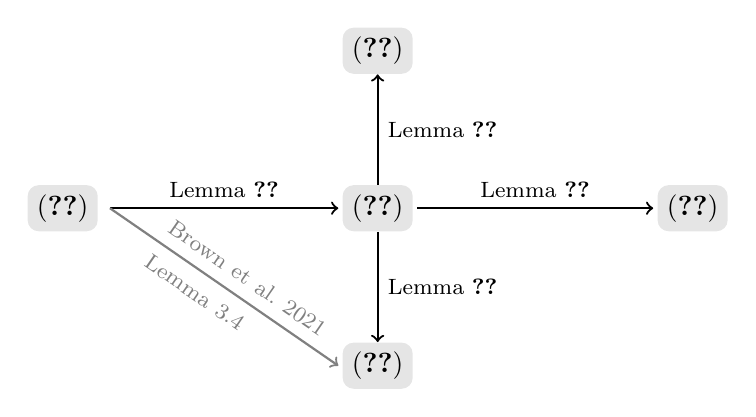
\begin{tikzpicture}[
mynode/.style={rectangle, rounded corners, fill=gray!20, minimum size=5mm},
]
% nodes
\node[mynode] at (0,0) {\eqref{eq:mainthmcond}};
\node[mynode] at (4,0) {\eqref{eq:kjjs_big_merger_bound}};
\node[mynode] at (4,2) {\eqref{eq:kjjs_binary_bound_2}};
\node[mynode] at (8,0) {\eqref{eq:kjjs_binary_bound_corrected}};
\node[mynode] at (4,-2) {\eqref{eq:kjjs_binary_bound}};
% arrows
\draw[->, thick] (0.6,0)-- node[anchor=south] 
        {\footnotesize{Lemma~\ref{lem:removeass2}}} (3.5,0);
\draw[->, thick] (4,0.3)-- node[anchor=west] 
        {\footnotesize{Lemma~\ref{lem:removeass3}}} (4,1.7);
\draw[->, thick] (4.5,0)-- node[anchor=south] 
        {\footnotesize{Lemma~\ref{thm:DNimpliescN_2}}} (7.5,0);
\draw[->, thick] (4,-0.3)-- node[anchor=west] 
        {\footnotesize{Lemma~\ref{thm:DNimpliescN}}} (4,-1.7);
\draw[->, thick, gray] (0.6,0)-- node[sloped, anchor=center, text width=2cm] 
        {\textcolor{gray}{\footnotesize{Brown~et~al.~2021 Lemma 3.4}}} (3.5,-2);
\end{tikzpicture}
\caption[Dependencies between conditions of Theorems \ref{thm:kjjs_mainthm} and \ref{thm:FDDconv}]{Dependencies between conditions of Theorems \ref{thm:kjjs_mainthm} and \ref{thm:FDDconv}. Arrows represent logical implication; labels on arrows indicate the lemma in which the implication is stated.
In \textcite[Lemma 3.4]{brown2021} the direct implication \eqref{eq:mainthmcond} $\Rightarrow$ \eqref{eq:kjjs_binary_bound} was proved, but here we will instead show that \eqref{eq:kjjs_big_merger_bound} $\Rightarrow$ \eqref{eq:kjjs_binary_bound}.
}
%The main condition of Theorem~\ref{thm:FDDconv}, \eqref{eq:mainthmcond}, implies the conditions \eqref{eq:kjjs_big_merger_bound}--\eqref{eq:kjjs_binary_bound} of Theorem~\ref{thm:kjjs_mainthm}.}
\label{fig:FDD_proof_dependencies}
\end{figure}


\begin{lemma} \label{lem:removeass3}
%$\eqref{eq:kjjs_big_merger_bound} \Rightarrow \eqref{eq:kjjs_binary_bound_2}$.\\
If for all $0 \leq s < t < \infty$
\begin{equation*}
\lim_{ N \rightarrow \infty } \E\Bigg[ \sum_{ r = \tau_N( s ) + 1 }^{ \tau_N( t ) } D_N( r ) \Bigg] = 0
\end{equation*}
then for all $0 \leq s < t < \infty$
\begin{equation*}
\lim_{ N \rightarrow \infty } \E\Bigg[ \sum_{ r = \tau_N( s ) + 1 }^{ \tau_N( t ) } c_N( r )^2 \Bigg] = 0 .
\end{equation*}
\end{lemma}

\begin{proof}
%It is sufficient to show that $c_N( t )^2 \leq D_N( t ) N/(N-1)$.
We have
\begin{align*}
c_N( t )^2 &= \frac{ 1 }{ N ( N - 1 ) ( N )_2 } \sum_{ i = 1 }^N ( \nu_t^{(i)})_2 \Bigg\{ \nu_t^{(i)} ( \nu_t^{(i)} - 1 ) + \sum_{\substack{j=1\\ j \neq i }}^N ( \nu_t^{(j)} )_2 \Bigg\} \\
&= \frac{ 1 }{ N ( N )_2 } \sum_{ i = 1 }^N ( \nu_t^{(i)} )_2 \Bigg\{ \frac{ \nu_t^{(i)} ( \nu_t^{(i)} - 1 ) }{ N - 1 } + \frac{ 1 }{ N - 1 } \sum_{\substack{j=1\\ j \neq i }}^N ( \nu_t^{(j)} )_2 \Bigg\} \\
&\leq \frac{ 1 }{ N ( N )_2 } \sum_{ i = 1 }^N ( \nu_t^{(i)})_2 \Bigg\{ \nu_t^{(i)} + \frac{ 1 }{ N - 1 } \sum_{\substack{j=1\\ j \neq i }}^N ( \nu_t^{(j)} )_2 \Bigg\} \\
&\leq \frac{ 1 }{ N ( N )_2 } \sum_{ i = 1 }^N ( \nu_t^{(i)})_2 \Bigg\{ \nu_t^{(i)} + \frac{ N / ( N - 1 ) }{ N } \sum_{\substack{j=1\\ j \neq i }}^N ( \nu_t^{(j)} )^2 \Bigg\} \\
&\leq \frac{ N / ( N - 1 ) }{ N ( N )_2 } \sum_{ i = 1 }^N ( \nu_t^{(i)})_2 \Bigg\{ \nu_t^{(i)} + \frac{ 1 }{ N } \sum_{\substack{j=1\\ j \neq i }}^N ( \nu_t^{(j)} )^2 \Bigg\} = \frac{ N }{ N - 1 } D_N( t )
\end{align*}
which is sufficient for the result.
\end{proof}


\begin{lemma} \label{thm:DNimpliescN}
%\eqref{eq:kjjs_big_merger_bound} $\Rightarrow$ \eqref{eq:kjjs_binary_bound}.\\
If for all $0 \leq s < t < \infty$
\begin{equation*}
\lim_{ N \rightarrow \infty } \E\Bigg[ \sum_{ r = \tau_N( s ) + 1 }^{ \tau_N( t ) } D_N( r ) \Bigg] = 0
\end{equation*}
then for all $ t \in \mathbb{N} $
\begin{equation*}
\lim_{ N \rightarrow \infty } \E[ c_N( t ) ] = 0 .
\end{equation*}
\end{lemma}

\begin{proof}
Fix $\epsilon>0$, and assume $N>2/\epsilon$.
Following \textcite{mohle2003}, define the events
\begin{equation}\label{eq:define_Ai_events}
A_i(t) := \{ \nu_t^{(i)} \leq N\epsilon \} .
\end{equation}
Then
\begin{align*}
c_N(t)
&= \frac{1}{(N)_2} \sum_{i=1}^N (\nu_t^{(i)})_2 [\1{A_i(t)} + \1{A_i(t)^c}] \\
&\leq \frac{N\epsilon}{(N)_2} \sum_{i=1}^N \nu_t^{(i)}
        + \sum_{i=1}^N \1{A_i(t)^c} \\
&= \frac{N\epsilon}{N-1} + \sum_{i=1}^N \1{A_i(t)^c} .
\end{align*}
Taking expectations and applying the generalised Markov inequality,
\begin{align*}
\E[c_N(t)]
&\leq \epsilon\ON + \sum_{i=1}^N \Prob[ \nu_t^{(i)} > N\epsilon ] \\
&\leq \epsilon\ON 
        + \sum_{i=1}^N \frac{\E[ (\nu_t^{(i)})_3 ]}{(N\epsilon)_3} \\
&\leq \epsilon\ON + \frac{N(N)_2}{(N\epsilon)_3} \E[ D_N(t) ] \\
&= \epsilon\ON + \epsilon^{-3}\ON \E[ D_N(t) ] \\
&\leq \epsilon\ON + \epsilon^{-3}\ON 
        \E\left[ \sum_{r=1}^t D_N(r) \right] \\
&\leq \epsilon\ON + \epsilon^{-3}\ON
        \E\left[ \sum_{r=\tau_N(0)+1}^{\tau_N(t)} D_N(r) \right] ,
\end{align*}
where $\ON$ is used as an asymptotic shorthand for any function that converges to $1$ as $N\to\infty$; for instance $\ON$ can be thought of $1 + O(N^{-1})$.
The last inequality is a consequence of $\tau_N(0)=0$ and $\tau_N(t) \geq t$ (Proposition~\ref{thm:cN_properties}\ref{item:cN_property6}).
Taking limits, 
\begin{equation*}
\lim_{N\to\infty} \E[c_N(t)] \leq \epsilon .
\end{equation*}
Since $\epsilon$ was arbitrary this concludes the proof.
\end{proof}


\begin{lemma} \label{thm:DNimpliescN_2}
%\eqref{eq:kjjs_big_merger_bound} $\Rightarrow$ \eqref{eq:kjjs_binary_bound_corrected}.\\
If for all $0 \leq s < t < \infty$
\begin{equation*}
\lim_{ N \rightarrow \infty } \E\Bigg[ \sum_{ r = \tau_N( s ) + 1 }^{ \tau_N( t ) } D_N( r ) \Bigg] = 0
\end{equation*}
then for all $ 0 < t < \infty $
\begin{equation*}
\lim_{ N \rightarrow \infty } \E[ c_N( \tau_N(t) ) ] = 0 .
\end{equation*}
\end{lemma}

\begin{proof}
Analogously to the proof of Lemma~\ref{thm:DNimpliescN}, we find
\begin{align*}
\E[c_N(\tau_N(t))]
&\leq \epsilon\ON + \sum_{i=1}^N \Prob[ \nu_{\tau_N(t)}^{(i)} > N\epsilon ] \\
&\leq \epsilon\ON + \epsilon^{-3}\ON \E\left[ D_N(\tau_N(t)) \right] \\
&\leq \epsilon\ON + \epsilon^{-3}\ON
        \E\left[ \sum_{r=\tau_N(0)+1}^{\tau_N(t)} D_N(r) \right] \\
&\underset{N\to\infty}{\longrightarrow} \epsilon
\end{align*}
which concludes the proof since $\epsilon$ was arbitrary.
\end{proof}


%\begin{lemma} \label{lem:removeass1}
%$\eqref{eq:mainthmcond} \Rightarrow \eqref{eq:kjjs_binary_bound}$.
%\end{lemma}
%\seb{This lemma is obsolete. In Figure \ref{fig:FDD_proof_dependencies} I'll just refer to the proof in BJJK.}
%\begin{proof}
%Following the proof of \textcite[Lemma 5.5]{mohle2003}, we fix $\varepsilon > 0$ and define the event $A_i = \{ \nu_t^{(i)} \leq N \varepsilon \}$.
%Now
%\begin{align}
%\Et[ c_N( t ) ] 
%&= \frac{ 1 }{ ( N )_2 } \sum_{ i = 1 }^N \Et[ ( \nu_t^{(i)} )_2] 
%        = \frac{ 1 }{ ( N )_2 } \sum_{ i = 1 }^N \Big\{ \Et[ ( \nu_t^{(i)} )_2 \1{ A_i } ] 
%        + \Et[ ( \nu_t^{(i)} )_2 \1{ A_i^c } ] \Big\} \notag \\
%&\leq \frac{ \varepsilon }{ N - 1 } \sum_{ i = 1 }^N \Et[ \nu_t^{(i)} \1{ A_i }] 
%        + \sum_{ i = 1 }^N \Et[\1{ A_i^c }] \notag \\
%&\leq ( 1 + O( N^{ -1 } ) ) \varepsilon + \sum_{ i = 1 }^N 
%        \Prob[ \nu_t^{(i)} > N \varepsilon \mid \mathcal{F}_{t-1}]. \label{cond_cN}
%\end{align}
%For $N \geq 3 / \varepsilon$, Markov's inequality yields
%\begin{align}
%\sum_{ i = 1 }^N \Prob[ \nu_t^{(i)} > N \varepsilon \mid \mathcal{F}_{t-1} ] 
%&\leq \frac{ 1 }{ ( N \varepsilon )_3 } \sum_{ i = 1 }^N 
%        \Et[ ( \nu_t^{(i)} )_3] 
%        = \frac{ ( 1 + O( N^{ -1 } ) ) }{ \varepsilon^3 ( N )_3 } 
%        \sum_{ i = 1 }^N \Et[ ( \nu_t^{(i)} )_3] \notag \\
%&\leq ( 1 + O( N^{ -1 } ) ) \frac{ b_N }{ \varepsilon^3 } \Et[ c_N( t )] . \label{markovs_ineq}
%\end{align}
%Substituting \eqref{markovs_ineq} into \eqref{cond_cN} and using $c_N( t ) \leq 1$ results in
%\begin{equation*}
%\Et[ c_N( t )]
%\leq ( 1 + O( N^{ -1 } ) ) 
%        \Bigg( \varepsilon + \frac{ b_N }{ \varepsilon^3 } \Bigg) \underset{N\to\infty}{\longrightarrow} \varepsilon
%\end{equation*}
%since $b_N \rightarrow 0$. 
%As $\varepsilon > 0$ was arbitrary, we have
%\begin{equation*}
%\E[ c_N( t ) ] 
%= \E\left[ \Et[ c_N( t ) ] \right] 
%\rightarrow 0
%\end{equation*}
%as $N \rightarrow \infty$.
%\end{proof}



\begin{lemma} \label{lem:removeass2}
%$\eqref{eq:mainthmcond} \Rightarrow \eqref{eq:kjjs_big_merger_bound}$.\\
If there exists a deterministic sequence $(b_N)_{N\geq1}$ such that\\ ${\lim}_{N\to\infty} b_N =0$ and
\begin{equation*}
\frac{1}{(N)_3} \sum_{i = 1}^N \Et[ (\nu_t^{(i)})_3 ]  \leq b_N \frac{1}{(N)_2} \sum_{i = 1}^N \Et[ (\nu_t^{(i)})_2 ]
\end{equation*}
for all $N$, uniformly in $t \in \mathbb{N}$,
then for all $0 \leq s < t < \infty$
\begin{equation*}
\lim_{ N \rightarrow \infty } \E\Bigg[ \sum_{ r = \tau_N( s ) + 1 }^{ \tau_N( t ) } D_N( r ) \Bigg] = 0 .
\end{equation*}
\end{lemma}

\begin{proof}
We decompose $D_N(t)$ as the sum of two terms and consider their filtered expectations. The first is
\begin{align}
\frac{ 1 }{ N ( N )_2 } \sum_{ i = 1 }^N \Et[ ( \nu_t^{(i)} )_2 \nu_t^{(i)} ] 
&= \frac{ 1 }{ N ( N )_2 } \sum_{ i = 1 }^N 
        \Et[ 2 ( \nu_t^{(i)} )_2 + ( \nu_t^{(i)} )_3] \notag\\
&\leq \frac{ 2 }{ N } \Et[ c_N( t )] + \frac{ 1 }{ ( N )_3 } \sum_{ i = 1 }^N 
        \Et[ ( \nu_t^{(i)} )_3 ] \notag\\
&\leq \Bigg(\frac{ 2 }{ N } + b_N \Bigg) \Et[ c_N( t ) ]. \label{DN_part_1}
\end{align}
The second is
\begin{align}
\frac{ 1 }{ N^2 ( N )_2 } \sum_{ j=1 }^N \sum_{ i \neq j } 
        \Et[ ( \nu_t^{(i)} )_2 ( \nu_t^{(j)} )^2] 
&= \frac{ 1 }{ N^2 ( N )_2 } \sum_{ j=1 }^N \sum_{ i \neq j } 
        \Et[ ( \nu_t^{(i)} )_2 ( \nu_t^{(j)} )_2 + ( \nu_t^{(i)} )_2 \nu_t^{(j)} ] \notag\\
&\leq \frac{ 1 }{ N^2 ( N )_2 } \sum_{ j=1 }^N \sum_{ i \neq j } 
        \Et[ ( \nu_t^{(i)} )_2 ( \nu_t^{(j)} )_2 ] + \frac{ \Et[ c_N( t ) ] }{ N } .         
        \label{DN_part_2}
\end{align}
Now, with the events $A_i(t)$ defined as in \eqref{eq:define_Ai_events},
\begin{align}
\sum_{ j=1 }^N \sum_{ i \neq j } \Et\{ ( \nu_t^{(i)} )_2 ( \nu_t^{(j)} )_2\} 
&= \sum_{ j=1 }^N \sum_{ i \neq j } 
        \Big\{ \Et[ ( \nu_t^{(i)} )_2 ( \nu_t^{(j)} )_2 \1{ A_i(t) } ]
        + \Et[ ( \nu_t^{(i)} )_2 ( \nu_t^{(j)} )_2 \1{ A_i(t)^c } ] \Big\} \notag\\
&\leq N \epsilon \sum_{ j=1 }^N \sum_{ i \neq j } 
        \Et[ \nu_t^{(i)} ( \nu_t^{(j)} )_2 \1{ A_i(t) } ] 
        + N^3 \sum_{ j=1 }^N \sum_{ i \neq j } \Et[ \nu_t^{(j)} \1{ A_i(t)^c } ] \notag\\
&\leq N^2 ( N )_2 \epsilon \Et[ c_N( t )] + N^4 \sum_{ i = 1 }^N 
        \Prob[ \nu_t^{(i)} > N \epsilon \mid \mathcal{F}_{t-1} ] . \label{DN_part_3}
\end{align}
For $N \geq 3 / \epsilon$, by the generalised Markov inequality,
\begin{align}\label{markovs_ineq}
\sum_{ i = 1 }^N \Prob( \nu_t^{(i)} > N \epsilon \mid \mathcal{F}_{t-1} ) &\leq \frac{ 1 }{ ( N \epsilon )_3 } \sum_{ i = 1 }^N \Et\{ ( \nu_t^{(i)} )_3\} = \frac{ \{ 1 + O( N^{ -1 } ) \} }{ \epsilon^3 ( N )_3 } \sum_{ i = 1 }^N \Et\{ ( \nu_t^{(i)} )_3\} \notag \\
&\leq \{ 1 + O( N^{ -1 } ) \} \frac{ b_N }{ \epsilon^3 } \Et\{ c_N( t )\}. 
\end{align}
Substituting \eqref{markovs_ineq} into \eqref{DN_part_3} gives
\begin{equation}
\sum_{ j=1 }^N \sum_{ i \neq j } \Et[ ( \nu_t^{(i)} )_2 ( \nu_t^{(j)} )_2 ]
\leq N^4 (1 + O( N^{ -1 } ))
        \Bigg( \epsilon + \frac{ b_N }{ \epsilon^3 } \Bigg) \Et[ c_N( t ) ] \label{DN_part_4}
\end{equation}
and substituting \eqref{DN_part_4} into \eqref{DN_part_2} gives
\begin{equation}
\frac{ 1 }{ N^2 ( N )_2 } \sum_{ j=1 }^N \sum_{ i \neq j } 
        \Et[ ( \nu_t^{(i)} )_2 ( \nu_t^{(j)} )^2 ] 
\leq \Bigg[ ( 1 + O( N^{ -1 } ) )
        \Big( \epsilon + \frac{ b_N }{ \epsilon^3 } \Big) 
        + \frac{ 1 }{ N } \Bigg] \Et[ c_N( t ) ]. \label{DN_last}
\end{equation}
Combining \eqref{DN_part_1} and \eqref{DN_last}, we have that
\begin{equation*}
\Et[ D_N(t) ] 
= \Bigg[ (1 + O( N^{ -1 } )) \Bigg( \epsilon + \frac{ b_N }{ \epsilon^3 } \Bigg) 
        + \frac{ 3 }{ N } + b_N \Bigg] \Et[ c_N(t) ] .
\end{equation*}
Finally, invoking Lemma~\ref{thm:kjjslemma2} twice gives
\begin{align*}
\E\Bigg[ \sum_{ r = \tau_N( s ) + 1 }^{ \tau_N( t ) } D_N( r ) \Bigg] 
&= \E\Bigg[ \sum_{ r = \tau_N( s ) + 1 }^{ \tau_N( t ) } \E_r[ D_N( r ) ] \Bigg] \\
&\leq \Big\{ (1 + O( N^{ -1 } )) 
        \Bigg( \epsilon + \frac{ b_N }{ \epsilon^3 } \Bigg) 
        + \frac{ 3 }{ N } + b_N \Bigg\}
        \E\Bigg[ \sum_{ r = \tau_N( s ) + 1 }^{ \tau_N( t ) } c_N( r ) \Bigg] \\
&\leq \Bigg\{ (1 + O( N^{ -1 } )) 
        \Bigg( \epsilon + \frac{ b_N }{ \epsilon^3 } \Bigg) 
        + \frac{ 3 }{ N } + b_N \Bigg\} ( t - s + 1 ) \\
& \underset{N\to\infty}{\longrightarrow} \epsilon ( t - s + 1 ),
\end{align*}
and recalling that $\epsilon > 0$ was arbitrary concludes the proof.
\end{proof}



\seb{Update KJJS references in the following to point to relevant places in the erratum. The proof is similar to \texttt{Dropbox/SMC\_Genealogies\slash Asymptotic\_genealogies\_of\_interacting\_particle\_systems\slash Post\_acceptance\_correction\slash Erratum/AOS/Round\_3/Indicators/full\_redraft.pdf}, from page 22. We need to refer to the KJJS erratum (once published), rather than the arXiv version which is not correct (lacking some indicators) and doesn't contain all the required results, then update equation and lemma numbers etc.\ as required.}


To complete the proof of Theorem~\ref{thm:FDDconv} it remains to show that condition \eqref{eq:kjjs_tau_bound} is unnecessary. We will show that Proposition~\ref{thm:pDelta_LB} can be used instead of \eqref{eq:kjjs_tau_bound} to obtain the same result.
The only part of \textcite[Proof of Theorem 1]{koskela2018} making use of condition \eqref{eq:kjjs_tau_bound} is the lower bound on finite-dimensional distributions of the genealogical process for paths involving single pair mergers only.
A slight modification of the argument allows a similar lower bound to be obtained via Proposition~\ref{thm:pDelta_LB} such that as $N\to\infty$ the bound coincides with the corresponding finite-dimensional distributions of the $n$-coalescent, as required.
The modified section of the proof is presented below, using the notation of \textcite{koskela2018} for ease of comparison.
\seb{Maybe I should actually write out a full proof of the new theorem?}

\begin{proof}
Let $\chi^\star_d$ be the conditional transition probability of a transition from state $\eta_{d-1}$ to state $\eta_d$ at times $\tau_N(t_{d-1})$ and $\tau_N(t_d)$ respectively, conditional on the offspring counts between those times $\nu^{(1:N)}_{\tau_N(t_{d-1}) +1} , \dots, \nu^{(1:N)}_{\tau_N(t_d)}$. 
This transition can happen via any valid path of merger events, but we restrict to paths involving binary mergers only, and denote by $\chi_d$ the conditional transition probability subject to this restriction.
Compared to \textcite[Proof of Theorem 1]{koskela2018}, the derivation of an upper bound on $\chi_d$ holds without modification, while the first step in the derivation of a lower bound \parencite[p.14]{koskela2018} involves the application of \textcite[Lemma 1 Case 1]{koskela2018} to bound $\chi_d$ from below and the subsequent application of \eqref{eq:kjjs_tau_bound}.
%The derivation of an upper bound on $\chi_d$ is unchanged from that in \textcite[Proof of Theorem 1]{koskela2018}.
%The first step in the derivation of a lower bound in \textcite[Proof of Theorem 1, p. 14]{koskela2018} consists of applying \textcite[Lemma 1]{koskela2018} to bound $\chi_d$ from below.
Instead, we apply Proposition~\ref{thm:pDelta_LB} to obtain, for sufficiently large $N$,
\begin{align*}
\chi_d 
&\geq \sum_{\substack{ s_1 < \ldots < s_{ \alpha } 
        \\= \tau_N( t_{ d - 1 } ) + 1 }}^{ \tau_N( t_d ) } 
        ( \tilde{ Q }^{ \alpha } )_{ \eta_{ d - 1 } \eta_d } 
        \Bigg( \prod_{ r = 1 }^{ \alpha } \I{ c_N(s_r) > \binom{n-2}{2} D_N(s_r) }
        \Bigg[ c_N( s_r ) - \binom{ n - 2 }{ 2 } \ON D_N( s_r ) \Bigg] \Bigg) \\
    &\hspace{2cm} \times \prod_{ \substack{ r = \tau_N( t_{ d - 1 } ) + 1 
        \\ r \notin \{ s_1, \ldots, s_\alpha \} }}^{ \tau_N( t_d ) } 
        \Bigg[ 1 - \tilde{B}_n \ON D_N( r ) 
        - \binom{ | \eta_{ d - 1 } | - | \{ i : s_i < r \} | }{ 2 } \ON c_N( r ) \Bigg] \\
    &\hspace{10cm}\times \I{ c_N(r) < (\tilde{B}_n + \binom{n}{2})^{-1} } .
\end{align*}
Here $\tilde{Q}$ is the matrix obtained from the generator $Q$ of Kingman's $n$-coalescent (see Definition \ref{def:kingman}) by setting the diagonal entries to 0.
The number of pair-merger steps required to transition from $\eta_{d-1}$ to $\eta_d$ is $\alpha = |\eta_{d-1}| - |\eta_d|$. The sequences $s_1,\dots,s_\alpha$ denote the times at which these pair-mergers happen. 
At the remaining times $r$ the partition is unchanged, and the bound of Proposition~\ref{thm:pDelta_LB} has been applied to the one-step transition probabilities corresponding to these identity transitions. 
The constant is $\tilde{B}_n := B_n\binom{n}{2}$ where $B_n$ is the constant defined in Proposition~\ref{thm:pDelta_LB}, and we have replaced $|\eta_d|$ by its upper bound $n$.
%A sum over an index vector of length zero should be interpreted as the identity operator here and in the following.

The rest of the proof proceeds as in \textcite{koskela2018}, albeit from this modified initial lower bound.
A multinomial expansion of the product on the second line, noting that $(\ON)^a = \ON$ for any $a\in\mathbb{R}$, yields
\begin{align*}
\chi_d 
&\geq \left( \prod_{r=\tau_N(t_{d-1})+1}^{\tau_N(t_d)}
        \I{ c_N(r) > \binom{n-2}{2} D_N(r) } 
        \I{ c_N(r) < (\tilde{B}_n + \binom{n}{2})^{-1} } \right) \\
    &\hspace{2cm}\times \sum_{ \beta = 0 }
        ^{ \tau_N( t_d ) - \tau_N( t_{ d - 1 } ) - \alpha } 
        ( \tilde{ Q }^{ \alpha } )_{ \eta_{ d - 1 } \eta_d } 
        \sum_{\substack{ ( \lambda, \mu ) \in \Pi_2( [ \alpha + \beta ] ) :
        \\ | \lambda | = \alpha }} \ON \\
    &\hspace{2cm}\times \sum_{\substack{ s_1 < \ldots < s_{ \alpha + \beta } 
        \\= \tau_N( t_{ d - 1 } ) + 1 }}^{ \tau_N( t_d ) } \Bigg( \prod_{ r \in \lambda }
        \Bigg[ c_N( s_r ) - \binom{ n - 2 }{ 2 } \ON D_N( s_r ) \Bigg] \Bigg)\\
    &\hspace{2cm}\times \prod_{ r \in \mu } \Bigg\{ - 
        \binom{ | \eta_{ d - 1 } | - | \{ i \in \lambda : i < r \} | }{ 2 } c_N( s_r ) 
        - \tilde{B}_n D_N( s_r ) \Bigg\}
\end{align*}
where $\Pi_i([n])$ denotes the set of partitions of $\{1, \dots,n\}$ into exactly $i$ blocks.
Expanding the product over $\lambda$ gives
\begin{align*}
\chi_d 
&\geq \left( \prod_{r=\tau_N(t_{d-1})+1}^{\tau_N(t_d)}
        \I{ c_N(r) > \binom{n-2}{2} D_N(r) } 
        \I{ c_N(r) < (\tilde{B}_n + \binom{n}{2})^{-1} } \right) \\
    &\hspace{2cm}\times \sum_{ \beta = 0 }
        ^{ \tau_N( t_d ) - \tau_N( t_{ d - 1 } ) - \alpha } 
        ( \tilde{ Q }^{ \alpha } )_{ \eta_{ d - 1 } \eta_d } 
        \sum_{\substack{ ( \lambda, \mu, \pi ) \in \Pi_3( [ \alpha + \beta ] ) :
        \\ | \mu | = \beta }} \binom{ n - 2 }{ 2 }^{ | \pi | } ( -1 )^{ | \pi | } \, \ON \\
        % ^{ \beta + | \pi | } \\
    &\qquad \times \sum_{\substack{ s_1 < \ldots < s_{ \alpha + \beta } 
        \\ = \tau_N( t_{ d - 1 } ) + 1 }}^{ \tau_N( t_d ) } 
        \Bigg\{ \prod_{ r \in \lambda } c_N( s_r ) \Bigg\} 
        \Bigg\{ \prod_{ r \in \pi }  D_N( s_r ) \Bigg\} \\
    &\qquad \times \prod_{ r \in \mu } \Bigg\{ - 
        \binom{ | \eta_{ d - 1 } | - | \{ i \in \lambda \cup \pi : i < r \} | }{ 2 } c_N( s_r ) 
        - \tilde{B}_n D_N( s_r ) \Bigg\}
\end{align*}
and expanding the product over $\mu$ results in
\begin{align*}
\chi_d 
&\geq \left( \prod_{r=\tau_N(t_{d-1})+1}^{\tau_N(t_d)}
        \I{ c_N(r) > \binom{n-2}{2} D_N(r) } 
        \I{ c_N(r) < (\tilde{B}_n + \binom{n}{2})^{-1} } \right) \\
    &\hspace{2cm}\times \sum_{ \beta = 0 }
        ^{ \tau_N( t_d ) - \tau_N( t_{ d - 1 } ) - \alpha } 
        ( \tilde{ Q }^{ \alpha } )_{ \eta_{ d - 1 } \eta_d } 
        \sum_{\substack{ ( \lambda, \mu, \pi, \sigma ) \in \Pi_4( [ \alpha + \beta ] ) :
        \\ | \mu | + | \sigma | = \beta }} \tilde{B}_n^{ | \sigma | } 
        \binom{ n - 2 }{ 2 }^{ | \pi | } ( -1 )^{ | \pi | + | \sigma | } \\
    &\qquad \times \ON % ^{ \beta + | \pi | } 
        \Bigg\{ \prod_{ r \in \mu } - 
        \binom{ | \eta_{ d - 1 } | - | \{ i \in \lambda \cup \pi : i < r \} | }{ 2 } \Bigg\} \\
    &\qquad \times \sum_{\substack{ s_1 < \ldots < s_{ \alpha + \beta } 
        \\ = \tau_N( t_{ d - 1 } ) + 1 }}^{ \tau_N( t_d ) } 
        \Bigg\{ \prod_{ r \in \lambda \cup \mu } c_N( s_r ) \Bigg\} 
        \prod_{ r \in \pi \cup \sigma }  D_N( s_r ) .
\end{align*}
Via a further multinomial expansion, the lower bound for the $k$-step transition probability can be written as
\begin{align*}
\lim_{ N \rightarrow \infty } \E\Bigg[ \prod_{ d = 1 }^k \chi_d \Bigg]
&\geq \lim_{ N \rightarrow \infty } 
        \E\Bigg[ \left( \prod_{r=\tau_N(t_0)+1}^{\tau_N(t_k)}
        \I{ c_N(r) > \binom{n-2}{2} D_N(r) } 
        \I{ c_N(r) < (\tilde{B}_n + \binom{n}{2})^{-1} } \right) \\
    &\qquad\times\sum_{ \beta_1 = 0 }^{ \infty } \ldots \sum_{ \beta_k = 0 }^{ \infty }         
        \sum_{\substack{ ( \lambda_1, \mu_1, \pi_1, \sigma_1 ) 
        \in \Pi_4( [ \alpha_1 + \beta_1 ] ):\\  | \mu_1 | + | \sigma_1 | = \beta_1 }}
        \ldots 
        \sum_{\substack{ ( \lambda_k, \mu_k, \pi_k, \sigma_k ) 
        \in \Pi_4( [ \alpha_k + \beta_k ] ) :\\ | \mu_k | + | \sigma_k | = \beta_k }} \\
    &\qquad \tilde{B}_n^{ \sum_{ d = 1 }^k | \sigma_d | } 
        \binom{ n - 2 }{ 2 }^{ \sum_{ d = 1 }^k| \pi_d | }
        ( -1 )^{ \sum_{ d = 1 }^k | \pi_d | + | \sigma_d | } \,
        \ON \\ % ^{ | \bm{ \beta } | + \sum_{ d = 1 }^k | \pi_d | } \\
    &\qquad \times \Bigg\{ \prod_{ d = 1 }^k 
        ( \tilde{ Q }^{ \alpha_d } )_{ \eta_{ d - 1 } \eta_d } 
        \prod_{ r \in \mu_d } - 
        \binom{ | \eta_{ d - 1 } | - | \{ i \in \lambda_d \cup \pi_d : i < r \} | }{ 2 } 
        \Bigg\} \\
    &\qquad \times 
        \sum_{\substack{ s_1^{ ( 1 ) } < \ldots < s_{ \alpha_1 + \beta_1 }^{ ( 1 ) } 
        \\= \tau_N( t_0 ) + 1 }}^{ \tau_N( t_1 ) } \ldots 
        \sum_{\substack{ s_1^{ ( k ) } < \ldots < s_{ \alpha_k + \beta_k }^{ ( k ) } 
        \\= \tau_N( t_{ k - 1 } ) + 1 }}^{ \tau_N( t_k ) } \\
    &\qquad \prod_{ d = 1 }^k 
        \I{ \tau_N( t_d ) - \tau_N( t_{ d - 1 } ) \geq \alpha_d + \beta_d } 
        \Bigg\{ \prod_{ r \in \lambda_d \cup \mu_d } c_N( s_r^{ ( d ) } ) \Bigg\} 
        \prod_{ r \in \pi_d \cup \sigma_d }  D_N( s_r^{ ( d ) } ) \Bigg].
\end{align*}
An argument completely analogous to that in \textcite[Appendix]{koskela2018} shows that passing the expectation and the limit through the infinite sums is justified, whereupon the contribution of terms with $ \sum_{ d = 1 }^k ( | \pi_d | + | \sigma_d | ) > 0$ vanishes.
To see why, follow the argument used to show that the contribution of multiple merger trajectories vanishes in the corresponding upper bound in \textcite{koskela2018}.
That leaves
\begin{align}
\lim_{ N \rightarrow \infty } \E\Bigg[ \prod_{ d = 1 }^k \chi_d \Bigg] 
&\geq \sum_{ \beta_1 = 0 }^{ \infty } \ldots \sum_{ \beta_k = 0 }^{ \infty }
        \sum_{\substack{ ( \lambda_1, \mu_1 ) \in \Pi_2( [ \alpha_1 + \beta_1 ] ) :
        \\ | \mu_1 | = \beta_1 }} \ldots 
        \sum_{\substack{ ( \lambda_k, \mu_k ) \in \Pi_2( [ \alpha_k + \beta_k ] ) :
        \\ | \mu_k | = \beta_k }} \notag \\
    &\qquad \Bigg\{ \prod_{ d = 1 }^k 
        ( \tilde{ Q }^{ \alpha_d } )_{ \eta_{ d - 1 } \eta_d }
        \prod_{ r \in \mu_d } - 
        \binom{ | \eta_{ d - 1 } | - | \{ i \in \lambda_d \cup \pi_d : i < r \} | }{ 2 } 
        \Bigg\} \notag \\
    &\qquad \times \lim_{ N \rightarrow \infty } \E\Bigg[ 
        \left( \prod_{r=\tau_N(t_{d-1})+1}^{\tau_N(t_d)}
        \I{ c_N(r) > \binom{n-2}{2} D_N(r) } 
        \I{ c_N(r) < (\tilde{B}_n + \binom{n}{2})^{-1} } \right) \notag\\
    &\qquad\times 
        \sum_{\substack{ s_1^{ ( 1 ) } < \ldots < s_{ \alpha_1 + \beta_1 }^{ ( 1 ) } 
        \\= \tau_N( t_0 ) + 1 }}^{ \tau_N( t_1 ) } \ldots 
        \sum_{\substack{ s_1^{ ( k ) } < \ldots < s_{ \alpha_k + \beta_k }^{ ( k ) } 
        \\= \tau_N( t_{ k - 1 } ) + 1 }}^{ \tau_N( t_k ) } \notag \\
    &\qquad \prod_{ d = 1 }^k 
        \I{ \tau_N( t_d ) - \tau_N( t_{ d - 1 } ) \geq \alpha_d + \beta_d } 
        \Bigg\{ \prod_{ r \in \lambda_d \cup \mu_d } c_N( s_r^{ ( d ) } ) \Bigg\} 
        \Bigg]. \label{eq1}
\end{align}
Recall \parencite[Eq (11)]{koskela2018}:
\begin{equation*}
\sum_{\substack{ ( \lambda, \mu ) \in \Pi_2( [ \alpha + \beta ] ) :
        \\ | \mu | = \beta }} ( \tilde{ Q }^{ \alpha } )_{ \eta_{ d - 1 } \eta_d } 
        \prod_{ r \in \mu } - 
        \binom{ | \eta_{ d - 1 } | - | \{ i \in \lambda \cup \pi : i < r \} | }{ 2 } 
= ( Q^{ \alpha + \beta } )_{ \eta_{ d - 1 } \eta_d } .
\end{equation*}
Applying this $k$ times in \eqref{eq1} yields
\begin{align*}
\lim_{ N \rightarrow \infty } \E\Bigg[ \prod_{ d = 1 }^k \chi_d \Bigg] 
&\geq \sum_{ \beta_1 = 0 }^{ \infty } \ldots \sum_{ \beta_k = 0 }^{ \infty } 
        \Bigg\{ \prod_{ d = 1 }^k 
        ( Q^{ \alpha_d + \beta_d } )_{ \eta_{ d - 1 } \eta_d } \Bigg\} \\
    &\qquad \times \lim_{ N \rightarrow \infty } \E\Bigg\{ 
        \left( \prod_{r=\tau_N(t_{d-1})+1}^{\tau_N(t_d)}
        \I{ c_N(r) > \binom{n-2}{2} D_N(r) } 
        \I{ c_N(r) < (\tilde{B}_n + \binom{n}{2})^{-1} } \right) \\
    &\hspace{3cm}\times \Bigg( \prod_{ d = 1 }^k 
        \I{ \tau_N( t_d ) - \tau_N( t_{ d - 1 } ) \geq \alpha_d + \beta_d } \Bigg) \\
    &\hspace{3cm}\times \sum_{\substack{ s_1^{ ( 1 ) } < \ldots < 
        s_{ \alpha_1 + \beta_1 }^{ ( 1 ) } \\= \tau_N( t_0 ) + 1 }}^{ \tau_N( t_1 ) } \ldots 
        \sum_{\substack{ s_1^{ ( k ) } < \ldots < s_{ \alpha_k + \beta_k }^{ ( k ) } 
        \\= \tau_N( t_{ k - 1 } ) + 1 }}^{ \tau_N( t_k ) } 
        \prod_{ d = 1 }^k \prod_{ r \in \lambda_d \cup \mu_d } 
        c_N( s_r^{ ( d ) } ) \Bigg\}.
\end{align*}
We now apply equations (14) and (15), respectively, of \textcite{koskela2018},  to those terms with a negative ($|\bm{\beta}|$ odd) and positive ($|\bm{\beta}|$ even) sign, respectively, to obtain
%\textcite[Eq (14)]{koskela2018} to those terms with a negative sign ($| \bm{ \beta } |$ odd) and \textcite[Eq (15)]{koskela2018} to those terms with a positive sign ($| \bm{ \beta } |$ even), and obtain
\begin{align*}
\lim_{ N \rightarrow \infty } \E\Bigg[ \prod_{ d = 1 }^k \chi_d \Bigg]
&\geq \sum_{ \beta_1 = 0 }^{ \infty } \ldots \sum_{ \beta_k = 0 }^{ \infty } 
        \Bigg\{ \prod_{ d = 1 }^k ( Q^{ \alpha_d + \beta_d } )_{ \eta_{ d - 1 } \eta_d } 
        \frac{ ( t_d - t_{ d - 1 } )^{ \alpha_d + \beta_d } }{ ( \alpha_d + \beta_d ) ! } 
        \Bigg\} \\
    &\qquad\times \lim_{ N \rightarrow \infty } \E\Bigg[ 
        \left( \prod_{r=\tau_N(t_{d-1})+1}^{\tau_N(t_d)}
        \I{ c_N(r) > \binom{n-2}{2} D_N(r) } 
        \I{ c_N(r) < (\tilde{B}_n + \binom{n}{2})^{-1} } \right) \\
    &\hspace{4cm}\times \Bigg( \prod_{ d = 1 }^k
        \I{ \tau_N( t_d ) - \tau_N( t_{ d - 1 } ) \geq \alpha_d + \beta_d } \Bigg) \Bigg] \\
&\geq \sum_{ \beta_1 = 0 }^{ \infty } \ldots \sum_{ \beta_k = 0 }^{ \infty } 
        \Bigg\{ \prod_{ d = 1 }^k ( Q^{ \alpha_d + \beta_d } )_{ \eta_{ d - 1 } \eta_d } 
        \frac{ ( t_d - t_{ d - 1 } )^{ \alpha_d + \beta_d } }{ ( \alpha_d + \beta_d ) ! } 
        \Bigg\} 
\end{align*}
where the expectation of the indicators converges to 1 due to \textcite[Equation (16)]{koskela2018} and Lemma~\ref{thm:indicators_cN}\seb{and Lemma~\ref{thm:lim_AandB}}. 
\seb{Or refer to \textcite[Equation (16)]{koskela2018} and Lemma 4 in the appendix of \texttt{full\_redraft.pdf}.}
\end{proof}


\chapter{Weak Convergence} %\seb{$\checkmark$} }
\label{ch:weakconv}

%\epigraph{
%At the age of twenty-one he wrote a treatise upon the Binomial Theorem, which has had a European vogue. On the strength of it he won the Mathematical Chair at one of our smaller universities, and had, to all appearances, a most brilliant career before him.
%}
%{\textsc{Sherlock Holmes}} %\\The Final Problem

In this chapter we present a weak convergence result which is identical to Theorem~\ref{thm:FDDconv} except that the mode of convergence is strengthened from convergence of the finite-dimensional distributions to weak convergence. 
Weak convergence is desirable because it implies convergence of a strictly larger class of functions of genealogies, granting access to the distributions of statistics such as the time to the sample MRCA, the total branch length, and the probability that the MRCA of a subsample is equal to the sample MRCA.
%\seb{okay, technically if this one is going to be a ``statistic'', I'm talking about the indicator on this event}. 

The extension from Theorem~\ref{thm:FDDconv} to weak convergence requires an additional tightness argument. The proof is rather long-winded since we do not have the strong assumptions on the dynamics of the interacting particle system that are exploited for example in \textcite{mohle1999}. The proof is broken down into a series of technical results which culminate in Theorem~\ref{thm:weakconv}. The overall structure of the proof is depicted graphically in Figure~\ref{fig:weakconv_structure}.


We start by defining a suitable metric space.
Let $\mathcal{P}_n$ be the space of partitions of $\{1,\dots,n\}$.
Denote by $\mathcal{D}$ the set of all functions mapping $[0,\infty)$ to $\mathcal{P}_n$ that are right-continuous with left limits.
Our rescaled genealogical process $(\mathcal{G}^{(n,N)}_{\tau_N(t)})_{t\geq0}$ and our encoding of the $n$-coalescent are piecewise-constant functions mapping time $t\in[0,\infty)$ to partitions, and thus live in the space $\mathcal{D}$.
Finally, equip the space $\mathcal{P}_n$ with the discrete metric,
\begin{equation*}
\rho(\xi,\eta) 
= 1- \delta_{\xi\eta} 
:= \begin{cases}
    0 &\text{if } \xi=\eta \\
    1 &\text{otherwise}
\end{cases}
\end{equation*}
for any $\xi, \eta \in \mathcal{P}_n$.


\begin{theorem}\label{thm:weakconv}
Let $\nu_t^{(1:N)}$ denote the offspring numbers in an interacting particle system satisfying \ref{standing_assumption} and such that, for any $N$ sufficiently large, for all finite $t$, $\Prob[ \tau_N(t) = \infty ] =0$. Suppose that there exists a deterministic sequence $(b_N)_{N\in\mathbb{N}}$ such that ${\lim}_{N\to\infty} b_N =0$ and%\amj{This bound comparse conditional expectations, so pedantically I suppose we should say that it holds almost surely?}
\begin{equation}\label{eq:mainthmcondition2}
\frac{1}{(N)_3} \sum_{i = 1}^N \Et\left[ (\nu_t^{(i)})_3 \right]  \leq b_N \frac{1}{(N)_2} \sum_{i = 1}^N \Et\left[ (\nu_t^{(i)})_2 \right]
\end{equation}
almost surely for all $N$, uniformly in $t \geq 1$.
Then the rescaled genealogical process $(G_{\tau_N(t)}^{(n,N)})_{t\geq0}$ converges weakly in $(\mathcal{D}, \rho)$
to Kingman's $n$-coalescent as $N \to \infty$.
\end{theorem}

\begin{proof}[Proof of Theorem~\ref{thm:weakconv}]
The structure of the proof follows \textcite{mohle1999}, albeit with considerable technical complication due to the dependence between generations (non-neutrality) in our model.
To make it digestible, the proof is broken down into a number of results which are organised into sections; the relationships between these are shown in Figure~\ref{fig:weakconv_structure}.

Since we already have convergence of the finite-dimensional distributions (Theorem~\ref{thm:FDDconv}), strengthening this to weak convergence requires relative compactness of the sequence of processes $\{ (G_{\tau_N(t)}^{(n,N)})_{t\geq0} \}_{N\in\mathbb{N}}$.

\textcite[Chapter 3, Corollary 7.4]{ethier1986} provide a necessary and sufficient condition for relative compactness: $\mathcal{P}_n$ is finite and therefore complete and separable, and the sample paths of $(G_{\tau_N(t)}^{(n,N)})_{t\geq0}$ live in $\mathcal{D}$, so the conditions of their corollary are satisfied.
The corollary states that the sequence of processes $\{ (G_{\tau_N(t)}^{(n,N)})_{t\geq0} \}_{N\in\mathbb{N}}$ is relatively compact if and only if the following two conditions hold:
\begin{enumerate}
\item \label{item:relcomp1} For every $\epsilon>0$, $t\geq 0$ there exists a compact set $\Gamma \subseteq \mathcal{P}_n$ such that
\begin{equation*}
\liminf_{N\to\infty} \Prob[ G_{\tau_N(t)}^{(n,N)} \in \Gamma ] 
\geq 1-\epsilon
\end{equation*}
\item \label{item:relcomp2} For every $\epsilon>0$, $t>0$ there exists $\delta>0$ such that
\begin{equation*}
\liminf_{N\to\infty} \Prob[ \omega(G_{\tau_N(\cdot)}^{(n,N)}, \delta, t) < \epsilon ] 
\geq 1-\epsilon
\end{equation*}
where $\omega$ is the modified modulus of continuity:
\begin{equation*}
\omega(G_{\tau_N(\cdot)}^{(n,N)}, \delta, t) := \inf \max_{i \in [K]} 
        \sup_{u,v \in [T_{i-1}, T_i)} \rho\left( 
        G_{\tau_N(u)}^{(n,N)}, G_{\tau_N(v)}^{(n,N)} \right)
\end{equation*}
with the infimum taken over all partitions of the form $0=T_0<T_1<\cdots <T_{K-1} <t \leq T_K$ (for any $K$) such that $\min_{i\in[K]} (T_i - T_{i-1}) > \delta$. 
\end{enumerate}
In our case, Condition~\ref{item:relcomp1} is satisfied automatically with $\Gamma = \mathcal{P}_n$, since $\mathcal{P}_n$ is finite and hence compact. 
Intuitively, Condition~\ref{item:relcomp2} ensures that the jumps of the process are well-separated. 
In our case where $\rho$ is the discrete metric, we see that $\rho( G_{\tau_N(u)}^{(n,N)}, G_{\tau_N(v)}^{(n,N)} )$ is equal to 1 if there is a jump between times $u$ and $v$, and 0 otherwise.
Taking the supremum and maximum then indicates whether there is a jump inside any of the intervals of the given partition; this can only be equal to zero if all of the jumps up to time $t$ occur exactly at the times $T_0, \dots, T_K$. 
The infimum over all allowed partitions, then, can only be equal to zero if no two jumps occur less than $\delta$ (unscaled) time apart, because of the restriction we placed on these partitions.

The proof is concentrated on proving Condition~\ref{item:relcomp2}.
To do this, we use a coupling with another process that contains all of the jumps of the genealogical process, with the addition of some extra jumps. This process is constructed in such a way that it can be shown to satisfy Condition 2, and hence so does the genealogical process.

Define $p_t := \max_{\xi\in \mathcal{P}_n} \{1 - p_{\xi\xi}(t)\} = 1 - p_{\Delta\Delta}(t)$, where $\Delta$ denotes the trivial partition of singletons $\{ \{1\},\dots, \{n\} \}$. For a proof that the maximum is attained at $\xi = \Delta$, see Lemma \ref{thm:maximum_pr}. 
Following \textcite{mohle1999}, we now construct the two-dimensional Markov process $(Z_t, S_t)_{t \in \mathbb{N}_0}$ on $\mathbb{N}_0 \times \mathcal{P}_n$ with transition probabilities
\begin{align}
\Prob[ Z_t = j , S_t = \eta \mid Z_{t-1} = i&, S_{t-1} = \xi, \mathcal{F}_\infty] \notag\\
&= \begin{cases}
1 - p_t &\quad \text{if } j=i \text{ and } \xi=\eta \\
p_{\xi\xi}(t) + p_t - 1  &\quad \text{if } j=i+1 \text{ and } \xi=\eta \\
p_{\xi\eta}(t) &\quad \text{if } j=i+1 \text{ and } \xi\neq\eta \\
0 &\quad \text{otherwise} 
\end{cases}
\label{eq:constructed_chain}
\end{align}
and initial state $Z_0=0$, $S_0 = \Delta$.
Unlike the corresponding process in \textcite{mohle1999}, in our case the transition probabilities depend on offspring counts, thus the process is only Markovian conditional on $\mathcal{F}_\infty$. It can be thought of as a Markov process in a random environment.

The construction is such that the marginal $(S_t)$ has the same distribution as the genealogical process of interest, and $(Z_t)$ has jumps at all the times $(S_t)$ does plus some extra jumps. The definition of $p_t$ ensures that the probability in the second case of \eqref{eq:constructed_chain} is non-negative, attaining the value zero when $\xi=\Delta$.
Furthermore, the transition probabilities (and hence jump times) of $(Z_t)$ do not depend on the current state.

Denote by $0=T_0^{(N)}<T_1^{(N)}<\dots$ the jump times of the rescaled process $(Z_{\tau_N(t)})_{t\geq0}$, and by $\varpi_i^{(N)} := T_i^{(N)} - T_{i-1}^{(N)}$ the corresponding holding times.

Suppose that for some fixed $\varpi_1^{(N)}, \dots, \varpi_m^{(N)}$ and $t>0$, there exists $m \in \mathbb{N}$ and $\delta >0$ such that
$\varpi_i^{(N)} > \delta$ for all $i\in \{1,\dots,m\}$, and
$T_m^{(N)} \geq t$.
Then
$K_N := \min\{i : T_i^{(N)} \geq t\}$
is well-defined with $1\leq K_N \leq m$,
and $T_1^{(N)} , \dots, T_{K_N}^{(N)}$ form a partition of the form required for Condition~\ref{item:relcomp2}.
Indeed $(Z_{\tau_N(\cdot)})$ is constant on every interval $[ T_{i-1}^{(N)} , T_i^{(N)} )$ by construction, so $\omega( (Z_{\tau_N(\cdot))} , \delta, t ) = 0$. 
We therefore have that
for each $m \in \mathbb{N}$ and $\delta >0$,
\begin{equation*}
\Prob[ \omega( (Z_{\tau_N(\cdot)}) , \delta, t ) < \epsilon ]
\geq \Prob[ T_m^{(N)} \geq t, \varpi_i^{(N)} > \delta \,\forall i\in \{1,\dots,m\} ] .
\end{equation*}
Thus a sufficient condition for Condition~\ref{item:relcomp2} is: 
for any $\epsilon>0$, $t>0$, there exist $m\in\mathbb{N}$, $\delta>0$ such that
\begin{equation}\label{eq:condition2b}
\liminf_{N\to\infty} 
        \Prob[ T_m^{(N)} \geq t, \varpi_i^{(N)} > \delta \,\forall i\in \{1,\dots,m\} ]
\geq 1-\epsilon .
\end{equation}
Since $T_m^{(N)} = \varpi_1^{(N)} + \cdots + \varpi_m^{(N)}$, there is a positive correlation between $T_m^{(N)}$ and each of the $\varpi_i^{(N)}$, and conditionally on $\mathcal{F}_\infty$ the $\varpi_i^{(N)}$'s are independent, so
\begin{align*}
\Prob[ &T_m^{(N)} \geq t , \varpi_i^{(N)} > \delta \,\forall i\in \{1,\dots,m\} 
        \mid \mathcal{F}_\infty ] \\
&= \Prob[ T_m^{(N)} \geq t \mid \varpi_i^{(N)} > \delta \,\forall i\in \{1,\dots,m\} 
        \mid \mathcal{F}_\infty ]
        \,\Prob[ \varpi_i^{(N)} > \delta \,\forall i\in \{1,\dots,m\} 
        \mid \mathcal{F}_\infty ] \\
&\geq \Prob[ T_m^{(N)} \geq t \mid \mathcal{F}_\infty ]
        \,\Prob[ \varpi_i^{(N)} > \delta \,\forall i\in \{1,\dots,m\} 
        \mid \mathcal{F}_\infty ] .
\end{align*}
Due to Lemma \ref{thm:holdingtimes_distn}, the limiting distributions of $\varpi_i^{(N)}$ are i.i.d. $\Exp(\alpha_n)$, where $\alpha_n := n(n-1)/2$, so
\begin{equation*}
\liminf_{N\to\infty} \Prob[ \varpi_i^{(N)} > \delta \,\forall i\in \{1,\dots,m\} ]
= (e^{-\alpha_n \delta})^m
\end{equation*}
and
\begin{equation*}
\liminf_{N\to\infty} \Prob[ T_m^{(N)} \geq t ]
= \liminf_{N\to\infty} \Prob[ \varpi_1^{(N)} + \cdots + \varpi_m^{(N)} \geq t ]
= e^{-\alpha_n t} \sum_{i=0}^{m-1} \frac{(\alpha_n t)^i}{i!} .
\end{equation*}
using the series expansion for the Erlang CDF \parencite[see for example][Chapter 15]{forbes2011}.
Hence 
\begin{align*}
&\liminf_{N\to\infty} 
        \Prob[ T_m^{(N)} \geq t, \varpi_i^{(N)} > \delta \,\forall i\in \{1,\dots,m\} ] \\
&\hspace{4cm}= \liminf_{N\to\infty} \E\left[ \Prob[ T_m^{(N)} \geq t, 
        \varpi_i^{(N)} > \delta \,\forall i\in \{1,\dots,m\} ] \right] \\
&\hspace{4cm}\geq \liminf_{N\to\infty} \E\left[ \Prob[ T_m^{(N)} \geq t 
        \mid \mathcal{F}_\infty ]
        \,\Prob[ \varpi_i^{(N)} > \delta \,\forall i\in \{1,\dots,m\} 
        \mid \mathcal{F}_\infty ] \right] \\
&\hspace{4cm}= \liminf_{N\to\infty} \left\{ \Prob[ T_m^{(N)} \geq t ]
        \,\Prob[ \varpi_i^{(N)} > \delta \,\forall i\in \{1,\dots,m\} ] \right\} \\
&\hspace{4cm}\geq (e^{-\alpha_n \delta})^m e^{-\alpha_n t} \sum_{i=0}^{m-1} 
        \frac{(\alpha_n t)^i}{i!} ,
\end{align*}
which can be made $\geq 1-\epsilon$ by taking $m$ sufficiently large and $\delta$ sufficiently small.
Since this argument applies for any $\epsilon$ and $t$, \eqref{eq:condition2b} and hence Condition~\ref{item:relcomp2} is satisfied, and the proof is complete.
\end{proof}




\begin{lemma}\label{thm:maximum_pr}
$\max_{\xi\in \mathcal{P}_n} (1 - p_{\xi\xi}(t)) = 1 - p_{\Delta\Delta}(t)$.
\end{lemma}

\begin{proof}
Consider any $\xi \in E$ consisting of $k$ blocks ($1\leq k\leq n-1$), and any $\xi^\prime\in E$ consisting of $k+1$ blocks. 
Setting $\eta=\xi$ in \eqref{eq:defn_pxieta},
%\parencite[Equation (1)]{koskela2018},
\begin{equation*}
p_{\xi\xi}(t) 
= \frac{1}{(N)_k} \sum_{\substack{i_1,\dots,i_k=1 \\ \text{all distinct}}}^N 
        \nu_t^{(i_1)} \cdots \nu_t^{(i_k)} .
\end{equation*}
Similarly,
\begin{align*}
p_{\xi^\prime\xi^\prime}(t) &= \frac{1}{(N)_{k+1}} 
        \sum_{\substack{i_1,\dots, i_{k+1} =1 \\ \text{all distinct}}}^N 
        \nu_t^{(i_1)} \cdots \nu_t^{(i_k)} \nu_t^{(i_{k+1})} \\
&= \frac{1}{(N)_k(N-k)} \sum_{\substack{i_1,\dots,i_k =1 \\ \text{all distinct}}}^N 
        \left\{ \nu_t^{(i_1)} \cdots \nu_t^{(i_k)} 
        \sum_{\substack{i_{k+1}=1 \\ \notin \{i_1,\ldots, i_k\} }}^N 
        \nu_t^{(i_{k+1})} \right\} .
\end{align*}
Discarding the zero summands,
\begin{equation*}
p_{\xi^\prime\xi^\prime}(t) 
    = \frac{1}{(N)_k(N-k)} \sum_{\substack{i_1,\dots,i_k =1 \\ \text{all distinct:} 
        \\ \nu_t^{(i_1)},\dots,\nu_t^{(i_k)} > 0 }}^N
        \left\{ \nu_t^{(i_1)} \cdots \nu_t^{(i_k)} 
        \sum_{\substack{i_{k+1}=1 \\ \notin \{i_1,\ldots, i_k\} }}^N 
        \nu_t^{(i_{k+1})} \right\} .
\end{equation*}
%For the summands such that $\nu_t^{(i_1)},\dots,\nu_t^{(i_k)}$ are all greater than or equal to $1$, the inner sum is
The inner sum is
\begin{equation*}
\sum_{\substack{i_{k+1}=1 \\ \notin \{i_1,\ldots, i_k\} }}^N \nu_t^{(i_{k+1})} 
    = \left\{ \sum_{i=1}^N \nu_t^{(i)} -  \sum_{i\in\{i_1,\dots,i_k\} } 
        \nu_t^{(i)} \right\}
    \leq N - k ,
\end{equation*}
since $\nu_t^{(i_1)},\dots,\nu_t^{(i_k)} $ are all at least 1.
%while if any of $\nu_t^{(i_1)},\dots,\nu_t^{(i_k)}$ are equal to $0$ then $p_{\xi^\prime\xi^\prime} =0$.
Hence
\begin{equation*}
p_{\xi^\prime\xi^\prime}(t)
    \leq  \frac{N-k}{(N)_k(N-k)} \sum_{\substack{i_1,\dots,i_k =1 
        \\ \text{all distinct:} \\ \nu_t^{(i_1)},\dots,\nu_t^{(i_k)} > 0 }}^N 
        \nu_t^{(i_1)} \cdots \nu_t^{(i_k)} 
    = p_{\xi\xi}(t) .
\end{equation*}
Thus $p_{\xi\xi}(t)$ is decreasing in the number of blocks of $\xi$, and is therefore minimised by taking $\xi = \Delta$, which uniquely achieves the maximum $n$ blocks. This choice in turn maximises $1-p_{\xi\xi}(t)$, as required.
\end{proof}




\begin{lemma}\label{thm:holdingtimes_distn}
The finite-dimensional distributions of $\varpi_1^{(N)} , \varpi_2^{(N)} , \dots$ converge as $N\to\infty$ to those of $\varpi_1, \varpi_2, \dots$, where the $\varpi_i$ are independent $\Exp(\alpha_n)$-distributed random variables.
\end{lemma}

\begin{proof}
There is a continuous bijection between the jump times $T_1^{(N)} ,T_2^{(N)},\dots$ and the holding times $\varpi_1^{(N)}, \varpi_2^{(N)}, \dots$, so convergence of the holding times to $\varpi_1, \varpi_2,\dots$ is equivalent to convergence of the jump times to $T_1, T_2, \dots$, where $T_i := \varpi_1+\dots+\varpi_i$. 
We will work with the jump times, following the structure of \textcite[Lemma 3.2]{mohle1999}.

The idea is to prove by induction that, for any $k\in\mathbb{N}$ and $t_1,\dots,t_k >0$,
\begin{equation}\label{eq:518}
\lim_{N\to\infty} \Prob[ T_1^{(N)} \leq t_1, \dots , T_k^{(N)} \leq t_k ]
= \Prob[ T_1 \leq t_1, \dots , T_k \leq t_k ] .
\end{equation}
Take the basis case $k=1$, for which
\begin{equation*}
\Prob[ T_1 \leq t ] 
= \Prob[ \varpi_1 \leq t ] = 1 - e^{-\alpha_n t}
\end{equation*}
and $T_1^{(N)} >t$ if and only if $Z$ has no jumps up to time $t$:
\begin{equation*}
\Prob[T_1^{(N)} >t]
= \E\left[ \Prob[ T_1^{(N)} >t \mid \mathcal{F}_\infty ] \right]
= \E\left[ \prod_{r=1}^{\tau_N(t)} (1-p_r) \right] .
\end{equation*}
Lemma \ref{thm:basis} shows that this probability converges to $e^{-\alpha_n t}$ as required.

For the induction step, assume that \eqref{eq:518} holds for some $k$. 
We have the following decomposition:
\begin{align*}
\Prob[ T_1^{(N)} \leq t_1, \dots , T_{k+1}^{(N)} \leq t_{k+1} ]
&= \Prob[ T_1^{(N)} \leq t_1, \dots , T_k^{(N)} \leq t_k ] \\
        &\qquad- \Prob[ T_1^{(N)} \leq t_1, \dots , T_k^{(N)} \leq t_k, T_{k+1}^{(N)} > t_{k+1} ] .
\end{align*}
The first term on the RHS converges to $\Prob[ T_1 \leq t_1, \dots , T_k \leq t_k ]$ by the induction hypothesis, and it remains to show that
\begin{equation*}
\lim_{N\to\infty} 
        \Prob[ T_1^{(N)} \leq t_1, \dots , T_k^{(N)} \leq t_k, T_{k+1}^{(N)} > t_{k+1} ]
= \Prob[ T_1\leq t_1, \dots , T_k \leq t_k, T_{k+1} > t_{k+1} ] .
\end{equation*}
As shown in \textcite{mohle1999},
\begin{equation*}
\Prob[ T_1\leq t_1, \dots , T_k \leq t_k, T_{k+1} > t_{k+1} ]
= \alpha_n^k e^{-\alpha_n t} 
        \sum_{\substack{i_1\leq \dots\leq i_{k-1}\\ \in \{0,\dots,k\} :
        \\ i_j \geq j \forall j}} 
        \prod_{j=1}^k \frac{(t_j - t_{j-1})^{i_j - i_{j-1}}}{(i_j - i_{j-1})! } ,
\end{equation*}
while the probability on the LHS can be written
\begin{align*}
&\Prob[ T_1^{(N)} \leq t_1, \dots , T_k^{(N)} \leq t_k, T_{k+1}^{(N)} > t_{k+1} ] \\
&\hspace{4cm}= \E\left[ \Prob[ T_1^{(N)} \leq t_1, \dots , T_k^{(N)} \leq t_k, T_{k+1}^{(N)} > t_{k+1} 
        \mid \mathcal{F}_\infty] \right] \\
&\hspace{4cm}= \E \left[ \sum_{\substack{r_1 <\dots< r_k :
        \\ r_i \leq \tau_N(t_i) \forall i}}
        \left( \prod_{i=1}^k p_{r_i} \right)
        \left( \prod_{\substack{r=1 \\ \notin \{r_1,\dots,r_k\} }}^{\tau_N(t)} 
        (1-p_r) \right) \right] .
\end{align*}
That is, there are jumps at some times $r_1, \dots, r_k$ and identity transitions at all other times.
A similar expression is derived in \textcite{mohle1999}, but here we have an additional outer expectation because the probabilities $p_r$ are random.
Lemmata \ref{thm:inductionUB} and \ref{thm:inductionLB} show that this probability converges to the correct limit.
This completes the induction.
\end{proof}


\begin{landscape}
\begin{figure}[ht]
\centering
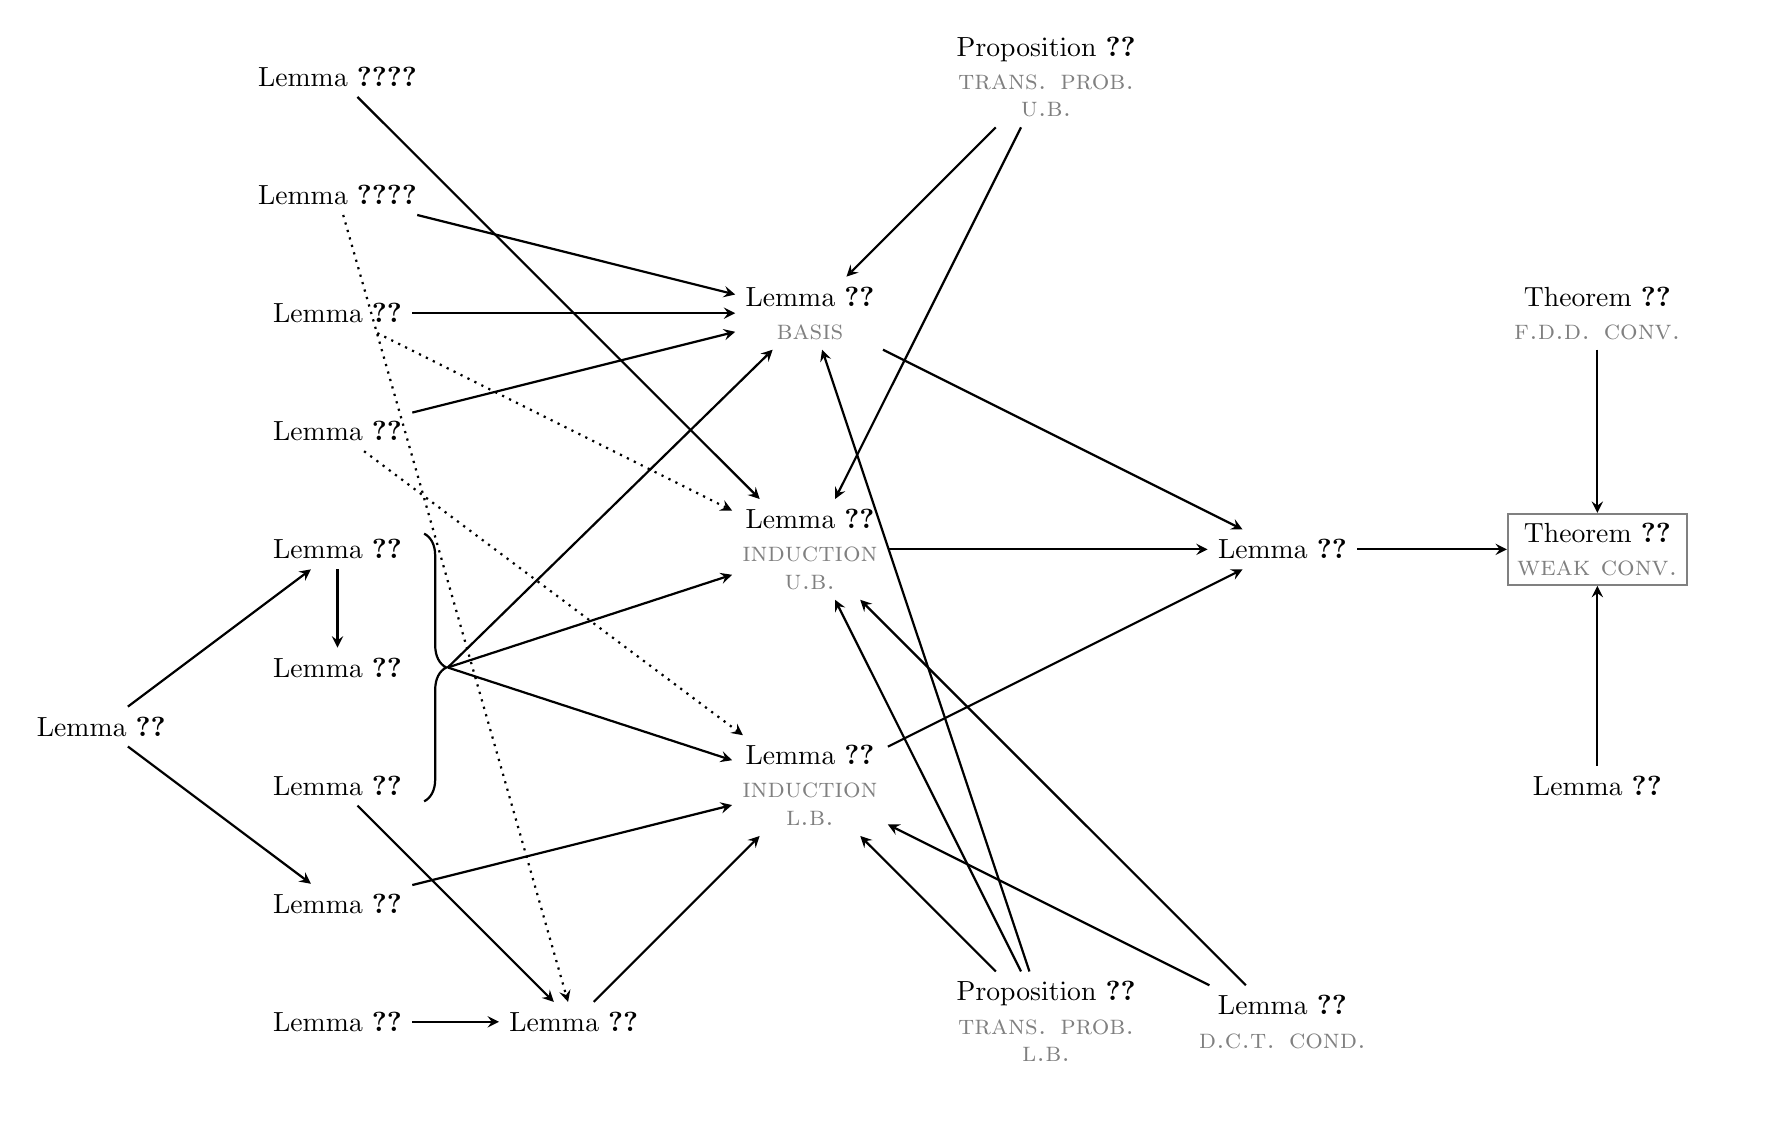
\begin{tikzpicture}[>=stealth, thick]
%% grid lines horizontal
%\draw[gray!20] (-15,0)--(6,0);
%\draw[gray!20] (-15,3)--(6,3);
%\draw[gray!20] (-15,6)--(6,6);
%\draw[gray!20] (-15,-3)--(6,-3);
%\draw[gray!20] (-15,-6)--(6,-6);
%% grid lines vertical
%\draw[gray!20] (0,6)--(0,-6);
%\draw[gray!20] (4,6)--(4,-6);
%\draw[gray!20] (-3,6)--(-3,-6);
%\draw[gray!20] (-6,6)--(-6,-6);
%\draw[gray!20] (-9,6)--(-9,-6);
%\draw[gray!20] (-12,6)--(-12,-6);
%\draw[gray!20] (-15,6)--(-15,-6);

% phantom line (to add space below figure)
\draw[white] (-15,-7)--(6,-7);

% nodes
\node[align=center,draw=gray] at (4,0) (c7r2) 
        {Theorem~\ref{thm:weakconv}\\[-3pt] \textcolor{gray}{\textsc{weak conv.}}};
\node[align=center] at (-6,-3) (c4r3) {Lemma~\ref{thm:inductionLB}\\[-3pt] 
        \textcolor{gray}{\textsc{induction}} \\[-5pt] \textcolor{gray}{\textsc{l.b.}} };
\node[align=center] at (-6,0) (c4r2) {Lemma~\ref{thm:inductionUB}\\[-3pt] 
        \textcolor{gray}{\textsc{induction}} \\[-5pt] \textcolor{gray}{\textsc{u.b.}} };
\node[align=center] at (-6,3) (c4r1) {Lemma~\ref{thm:basis}\\[-3pt] 
        \textcolor{gray}{\textsc{basis}} };
\node[align=center] at (4,3) (c7r1) {Theorem~\ref{thm:FDDconv}\\[-3pt] \textcolor{gray}{\textsc{f.d.d. conv.}} };
\node at (-15,-2.25) (c1r1) {Lemma~\ref{thm:kjjslemma2}};
\node at (4,-3) (c7r3) {Lemma~\ref{thm:maximum_pr}};
\node at (0,0) (c6r1) {Lemma~\ref{thm:holdingtimes_distn}};
\node[align=center] at (-3,6) (c5r1) {Proposition~\ref{thm:pDelta_LB}\\[-3pt] 
        \textcolor{gray}{\textsc{trans. prob.}} \\[-5pt] \textcolor{gray}{\textsc{u.b.}} };
\node[align=center] at (-3,-6) (c5r2) {Proposition~\ref{thm:pDelta_UB}\\[-3pt] 
        \textcolor{gray}{\textsc{trans. prob.}} \\[-5pt] \textcolor{gray}{\textsc{l.b.}} };
\node[align=center] at (0,-6) (c6r2) {Lemma~\ref{thm:DCT_Fubini}\\[-3pt] 
        \textcolor{gray}{\textsc{d.c.t. cond.}} };
\node at (-9,-6) (c3r1) {Lemma~\ref{thm:induction_sumprodcN}};
\node at (-12,6) (c2r1) {Lemma~\ref{thm:sumprod1}\ref{thm:sumprod1_a}};
\node at (-12,4.5) (c2r2) {Lemma~\ref{thm:sumprod1}\ref{thm:sumprod1_b}};
\node at (-12,3) (c2r3) {Lemma~\ref{thm:sumprod2}};
\node at (-12,1.5) (c2r4) {Lemma~\ref{thm:sumprod3}};
\node at (-12,-1.5) (c2r6) {Lemma~\ref{thm:indicators_tau}};
\node at (-12,0) (c2r5) {Lemma~\ref{thm:indicators_cN}};
\node at (-12,-3) (c2r7) {Lemma~\ref{thm:lim_AandB}};
\node at (-12,-4.5) (c2r8) {Lemma~\ref{thm:indicators_DN}};
\node at (-12,-6) (c2r9) {Lemma~\ref{thm:indicators_c2}};

% brace
\draw[decorate, decoration={brace, amplitude=8}] (-10.9,0.2)--(-10.9, -3.2);

% arrows from column 1
\draw[->] (c1r1)--(c2r8);
\draw[->] (c1r1)--(c2r5);
% arrows from column 2
\draw[->] (c2r5)--(c2r6);
\draw[->] (c2r1)--(c4r2);
\draw[->] (c2r2)--(c4r1);
\draw[->, dotted] (c2r2)--(c3r1);
\draw[->] (c2r3)--(c4r1);
\draw[->, dotted] (c2r3)--(c4r2);
\draw[->] (c2r4)--(c4r1);
\draw[->, dotted] (c2r4)--(c4r3);
\draw[->] (c2r8)--(c4r3);
\draw[->] (c2r9)--(c3r1);
\draw[->] (c2r7)--(c3r1);
% arrows from brace
\draw[->] (-10.6, -1.5)--(c4r1);
\draw[->] (-10.6, -1.5)--(c4r2);
\draw[->] (-10.6, -1.5)--(c4r3);
% arrows from column 3
\draw[->] (c3r1)--(c4r3);
% arrows from column 4
\draw[->] (c4r1)--(c6r1);
\draw[->] (c4r2)--(c6r1);
\draw[->] (c4r3)--(c6r1);
% arrows from column 5
\draw[->] (c5r1)--(c4r1);
\draw[->] (c5r1)--(c4r2);
\draw[->] (c5r2)--(c4r1);
\draw[->] (c5r2)--(c4r2);
\draw[->] (c5r2)--(c4r3);
% arrows from column 6
\draw[->] (c6r1)--(c7r2);
\draw[->] (c6r2)--(c4r2);
\draw[->] (c6r2)--(c4r3);
% arrows from column 7
\draw[->] (c7r1)--(c7r2);
\draw[->] (c7r3)--(c7r2);
\end{tikzpicture}
\caption[Structure of weak convergence proof]{Graph showing dependencies between the lemmata used to prove weak convergence. Dotted arrows indicate dependence via a slight modification of the preceding lemma.}
%Dependencies preceding Theorem~\ref{thm:FDDconv} are not shown; these are shown in Figure~??\seb{draw a corresponding figure for fdd proof, or delete this sentence?}.}
\label{fig:weakconv_structure}
\end{figure}
\end{landscape}




\section{Bounds on sum-products}
We start by proving some upper and lower bounds on sums of products of various quantities, which appear from our bounds on $p_r$ (Propositions~\ref{thm:pDelta_LB} and \ref{thm:pDelta_UB}). These sum-product bounds will be applied multiple times in the lemmata of this chapter.

\begin{lemma}\label{thm:sumprod1}
Fix $t>0$, $l\in\mathbb{N}$.
\begin{enumerate}[label=(\alph*)]
\item \label{thm:sumprod1_a} %\hspace{0.2cm}
$\begin{aligned}
\sum_{\substack{ s_1, \dots, s_l =1 \\ \text{\normalfont{all distinct}} }}^{\tau_N(t)}
        \prod_{j=1}^l c_N(s_j)
    \leq (t+1)^l
\end{aligned}$
\item \label{thm:sumprod1_b} %\hspace{0.2cm}
$\begin{aligned}
t^l - \left( \sum_{s=1}^{\tau_N(t)} c_N(s)^2 \right) \binom{l}{2} (t+1)^{l-2} 
    \leq \sum_{\substack{ s_1, \dots, s_l =1 \\ \text{\normalfont{all distinct}} }}
        ^{\tau_N(t)} \prod_{j=1}^l c_N(s_j)
    \leq t^l + c_N(\tau_N(t)) (t+1)^l
\end{aligned}$
\end{enumerate}
\end{lemma}

\begin{proof} \textbf{\ref{thm:sumprod1_a}}
Firstly, we have the inequality
\begin{equation*}
\sum_{\substack{ s_1, \dots, s_l =1 \\ \text{all distinct} }}^{\tau_N(t)}
        \prod_{j=1}^l c_N(s_j)
\leq \left( \sum_{s=0}^{\tau_N(t)} c_N(s) \right)^l ,
\end{equation*}
as can be seen by considering the multinomial expansion of the RHS.
Applying Proposition~\ref{thm:cN_properties}\ref{item:cN_property4},
\begin{equation}\label{eq:039}
\sum_{\substack{ s_1, \dots, s_l =1 \\ \text{all distinct} }}^{\tau_N(t)}
        \prod_{j=1}^l c_N(s_j)
\leq (t+1)^l .
\end{equation}
\textbf{\ref{thm:sumprod1_b}}
As pointed out in \textcite[Equation (8)]{koskela2018}, 
\begin{equation}\label{eq:002}
\sum_{\substack{ s_1, \dots, s_l =1 \\ \text{all distinct} }}^{\tau_N(t)} 
        \prod_{j=1}^l c_N(s_j)
\geq \left( \sum_{s=0}^{\tau_N(t)} c_N(s) \right)^l
        - \binom{l}{2} \left( \sum_{s=0}^{\tau_N(t)} c_N(s)^2 \right)
        \left( \sum_{s=0}^{\tau_N(t)} c_N(s) \right)^{l-2} .
\end{equation}
Applying Proposition~\ref{thm:cN_properties}\ref{item:cN_property4} on the RHS of \eqref{eq:002} yields the lower bound.

For the upper bound we have
\begin{equation*}
\sum_{\substack{ s_1, \dots, s_l =1 \\ \text{all distinct} }}^{\tau_N(t)} 
        \prod_{j=1}^l c_N(s_j)
\leq \left( \sum_{s=0}^{\tau_N(t)} c_N(s) \right)^l
\leq \left( \sum_{s=0}^{\tau_N(t) -1} c_N(s) + c_N(\tau_N(t)) \right)^l
\leq \left[ t + c_N(\tau_N(t)) \right]^l ,
\end{equation*}
using the definition of $\tau_N$.
A binomial expansion yields
\begin{equation*}
\left[ t + c_N(\tau_N(t)) \right]^l
= t^l + \sum_{i=0}^{l-1} \binom{l}{i} t^i c_N(\tau_N(t))^{l-i}
= t^l + c_N(\tau_N(t)) \sum_{i=0}^{l-1} \binom{l}{i} t^i c_N(\tau_N(t))^{l-1-i} ,
\end{equation*}
then by Proposition~\ref{thm:cN_properties}\ref{item:cN_property1},
\begin{equation*}
\sum_{i=0}^{l-1} \binom{l}{i} t^i c_N(\tau_N(t))^{l-1-i}
\leq \sum_{i=0}^{l-1} \binom{l}{i} t^i
\leq (t+1)^l .
\end{equation*}
Putting this together yields the upper bound.
\end{proof}


\begin{lemma}\label{thm:sumprod2}
Fix $t>0$, $l\in\mathbb{N}$.
%Let $B$ be a positive constant which may depend on $n$.
Then, for any constant $B>0$,
\begin{align*}
&\sum_{\substack{ s_1, \dots, s_l =1 \\ \text{\normalfont{all distinct}} }}^{\tau_N(t)} 
        \prod_{j=1}^l \left[ c_N(s_j) + B D_N(s_j) \right] \\
&\hspace{4cm}\leq \sum_{\substack{ s_1, \dots, s_l =1 \\ \text{\normalfont{all distinct}} }}^{\tau_N(t)} 
        \prod_{j=1}^l c_N(s_j)
        + \left( \sum_{s=1}^{\tau_N(t)} D_N(s) \right) (t+1)^{l-1} (1+B)^l .
\end{align*}
\end{lemma}

\begin{proof}
We start with a binomial expansion:
\begin{align}
\sum_{\substack{ s_1, \dots, s_l =1 \\ \text{all distinct} }}^{\tau_N(t)} 
        \prod_{j=1}^l \left[ c_N(s_j) + B D_N(s_j) \right]
&= \sum_{\substack{ s_1, \dots, s_l =1 \\ \text{all distinct} }}^{\tau_N(t)} 
        \sum_{\mathcal{I} \subseteq [l]}
        B^{l-|\mathcal{I}|} \left( \prod_{i\in\mathcal{I}} c_N(s_i) \right)
        \left( \prod_{j\notin\mathcal{I}} D_N(s_j) \right) \notag\\
&= \sum_{\mathcal{I} \subseteq [l]} B^{l-|\mathcal{I}|}
        \sum_{\substack{ s_1, \dots, s_l =1 \\ \text{all distinct} }}^{\tau_N(t)}
        \left( \prod_{i\in\mathcal{I}} c_N(s_i) \right)
        \left( \prod_{j\notin\mathcal{I}} D_N(s_j) \right) \label{eq:010}
\end{align}
where $[l] := \{1,\dots,l\}$. Since we are summing over all permutations of $s_1,\dots,s_l$, the particular partition of $\{1,\dots,l\}$ into $(\mathcal{I},\mathcal{I}^c)$ is not important; only the size of $\mathcal{I}$ matters. We may therefore replace the sum over $\mathcal{I}$ with a sum over $I:= |\mathcal{I}|$ and, without loss of generality, set $\mathcal{I} = \{1,\dots,I\}$:
%we may arbitrarily choose an ordering for $\{1,\dots,l\}$ such that $\mathcal{I} = \{ 1,\dots, |\mathcal{I}| \}$:
\begin{align*}
\sum_{\mathcal{I} \subseteq [l]} B^{l-|\mathcal{I}|}
        \sum_{\substack{ s_1, \dots, s_l =1 \\ \text{all distinct} }}^{\tau_N(t)}
        &\left( \prod_{i\in\mathcal{I}} c_N(s_i) \right)
        \left( \prod_{j\notin\mathcal{I}} D_N(s_j) \right) \\
&= \sum_{I=0}^l \binom{l}{I} B^{l-I} 
        \sum_{\substack{ s_1, \dots, s_l =1 \\ \text{all distinct} }}^{\tau_N(t)}
        \left( \prod_{i=1}^I c_N(s_i) \right)
        \left( \prod_{j=I+1}^l D_N(s_j) \right) .
\end{align*}
Separating the term $I=l$,
\begin{align}
\sum_{I=0}^l \binom{l}{I} &B^{l-I} 
        \sum_{\substack{ s_1, \dots, s_l =1 \\ \text{all distinct} }}^{\tau_N(t)}
        \left( \prod_{i=1}^I c_N(s_i) \right)
        \left( \prod_{j=I+1}^l D_N(s_j) \right) \notag\\
&= \sum_{\substack{ s_1, \dots, s_l =1 \\ \text{all distinct} }}^{\tau_N(t)}
        \prod_{j=1}^l c_N(s_j)
    + \sum_{I=0}^{l-1} \binom{l}{I} B^{l-I} 
        \sum_{\substack{ s_1, \dots, s_l =1 \\ \text{all distinct} }}^{\tau_N(t)}
        \left( \prod_{i=1}^I c_N(s_i) \right) \left( \prod_{j=I+1}^l D_N(s_j) \right). \label{eq:012}
\end{align}
In the second term on the RHS, there is always at least one $D_N$ term, so using Proposition~\ref{thm:cN_properties}\ref{item:cN_property2} we can write
\begin{align}
\sum_{I=0}^{l-1}\binom{l}{I} B^{l-I} 
        &\sum_{\substack{ s_1, \dots, s_l =1 \\ \text{all distinct} }}^{\tau_N(t)}
        \left( \prod_{i=1}^I c_N(s_i) \right) \left( \prod_{j=I+1}^l D_N(s_j) \right) \notag\\
&\leq \sum_{I=0}^{l-1}\binom{l}{I} B^{l-I} 
        \sum_{\substack{ s_1, \dots, s_l =1 \\ \text{all distinct} }}^{\tau_N(t)}
        \left( \prod_{i=1}^{l-1} c_N(s_i) \right) D_N(s_l) \notag\\
&\leq \sum_{I=0}^{l-1}\binom{l}{I} B^{l-I} 
        \left( \sum_{\substack{ s_1, \dots, s_l =1 \\ \text{all distinct} }}^{\tau_N(t)}
        \prod_{i=1}^{l-1} c_N(s_i) \right) 
        \sum_{s_l=1}^{\tau_N(t)} D_N(s_l) \notag\\
&\leq \sum_{I=0}^{l-1}\binom{l}{I} B^{l-I} (t+1)^{l-1}
        \sum_{s=1}^{\tau_N(t)} D_N(s) \label{eq:013}
\end{align}
using \eqref{eq:039}.
Finally, by the Binomial Theorem,
\begin{equation}\label{eq:014}
\sum_{I=0}^{l-1}\binom{l}{I} B^{l-I} (t+1)^{l-1}
        \sum_{s=1}^{\tau_N(t)} D_N(s)
\leq \left( \sum_{s=1}^{\tau_N(t)} D_N(s) \right) (t+1)^{l-1} (1+B)^l ,
\end{equation}
which, together with \eqref{eq:012}, concludes the proof.
\end{proof}


\begin{lemma}\label{thm:sumprod3}
Fix $t>0$, $l\in\mathbb{N}$.
%Let $B$ be a positive constant which may depend on $n$.
Then, for any constant $B>0$,
\begin{align*}
&\sum_{\substack{ s_1, \dots, s_l =1 \\ \text{\normalfont{all distinct}} }}^{\tau_N(t)} 
        \prod_{j=1}^l \left[ c_N(s_j) - B D_N(s_j) \right] \\
&\hspace{4cm}\geq \sum_{\substack{ s_1, \dots, s_l =1 \\ \text{\normalfont{all distinct}} }}^{\tau_N(t)} 
        \prod_{j=1}^l c_N(s_j)
        - \left( \sum_{s=1}^{\tau_N(t)} D_N(s) \right) (t+1)^{l-1} (1+B)^l .
\end{align*}
\end{lemma}

\begin{proof}
A binomial expansion and subsequent manipulation as in \eqref{eq:010}--\eqref{eq:012} gives
\begin{align*}
\sum_{\substack{ s_1, \dots, s_l =1 \\ \text{all distinct} }}^{\tau_N(t)} 
        &\prod_{j=1}^l 
        \left[ c_N(s_j) - B D_N(s_j) \right] \\
&= \sum_{\mathcal{I} \subseteq [l]} (-B)^{l-|\mathcal{I}|}
        \sum_{\substack{ s_1, \dots, s_l =1 \\ \text{all distinct} }}^{\tau_N(t)}
        \left( \prod_{i\in\mathcal{I}} c_N(s_i) \right)
        \left( \prod_{j\notin\mathcal{I}} D_N(s_j) \right) \\
&= \sum_{I=0}^l \binom{l}{I} (-B)^{l-I} 
        \sum_{\substack{ s_1, \dots, s_l =1 \\ \text{all distinct} }}^{\tau_N(t)}
        \left( \prod_{i=1}^I c_N(s_i) \right)
        \left( \prod_{j=I+1}^l D_N(s_j) \right) \\
&= \sum_{\substack{ s_1, \dots, s_l =1 \\ \text{all distinct} }}^{\tau_N(t)} 
        \prod_{j=1}^l c_N(s_j)
        + \sum_{I=0}^{l-1} \binom{l}{I} (-B)^{l-I} 
        \sum_{\substack{ s_1, \dots, s_l =1 \\ \text{all distinct} }}^{\tau_N(t)}
        \left( \prod_{i=1}^I c_N(s_i) \right) 
        \left( \prod_{j=I+1}^l D_N(s_j) \right) \\
&\geq \sum_{\substack{ s_1, \dots, s_l =1 \\ \text{all distinct} }}^{\tau_N(t)} 
        \prod_{j=1}^l c_N(s_j)
        - \sum_{I=0}^{l-1} \binom{l}{I} B^{l-I} 
        \sum_{\substack{ s_1, \dots, s_l =1 \\ \text{all distinct} }}^{\tau_N(t)}
        \left( \prod_{i=1}^I c_N(s_i) \right) \left( \prod_{j=I+1}^l D_N(s_j) \right)
\end{align*}
where the last inequality just multiplies some positive terms by $-1$.
Then \eqref{eq:013}--\eqref{eq:014} can be applied directly (noting that an upper bound on negative terms gives a lower bound overall):
\begin{align*}
&- \sum_{I=0}^{l-1} \binom{l}{I} B^{l-I} 
        \sum_{\substack{ s_1, \dots, s_l =1 \\ \text{all distinct} }}^{\tau_N(t)}
        \left( \prod_{i=1}^I c_N(s_i) \right) \left( \prod_{j=I+1}^l D_N(s_j) \right) \\
&\hspace{2cm}\geq - \left( \sum_{s=1}^{\tau_N(t)} D_N(s) \right) (t+1)^{l-1} (1+B)^l 
\end{align*}
which concludes the proof.
\end{proof}




\section{Main components of induction argument}
This section contains the technical aspects of the proof of Lemma~\ref{thm:holdingtimes_distn}, which establishes the limiting distributions of holding times of the coupled process, via an induction argument.
This section is split into four lemmata: the first (Lemma~\ref{thm:basis}) is used in the basis step and the others in the induction step. The induction step is established by combining upper and lower bounds, proved in Lemmata~\ref{thm:inductionUB} and \ref{thm:inductionLB} respectively. Lemma~\ref{thm:induction_sumprodcN} is a technical result which is common to both the upper and lower bounds, determining the limit as $N\to\infty$ of a certain expectation that arises in both bounds.

Recall that the following conditions are all consequences of \eqref{eq:mainthmcondition2}: for all $t>s>0$,
\begin{align}
\E \left[ c_N(\tau_N(t)) \right] &\rightarrow 0 \label{eq:BJJK_eq3.3}\\
\E\left[ \sum_{r=\tau_N(s)+1}^{\tau_N(t)} c_N(r)^2 \right] &\rightarrow 0
        \label{eq:BJJK_eq3.5}\\
\E\left[ \sum_{r=\tau_N(s)+1}^{\tau_N(t)} D_N(r) \right] &\rightarrow 0
        \label{eq:BJJK_eq3.4}
\end{align}
as $N\to\infty$. (See Lemmata~\ref{lem:removeass3}, \ref{thm:DNimpliescN} and \ref{lem:removeass2} for proofs.)
%Also recall the following properties from Proposition~\ref{thm:cN_properties}:
%\begin{align}
%& c_N(t) , D_N(t) \in [0,1] \label{eq:cN_property1}\\
%& D_N(t) \leq c_N(t) \label{eq:cN_property2}\\
%& t^\prime
%    \leq \sum_{r=1}^{\tau_N(t^\prime)} c_N(r) 
%    \leq t^\prime +1 .\label{eq:cN_property4}
%\end{align}



\begin{lemma}[Basis step]\label{thm:basis}
Assume \eqref{eq:mainthmcondition2} holds.
For any $0 < t < \infty$,
\begin{equation*}
\lim_{N\to\infty} \E\left[ \prod_{r=1}^{\tau_N(t)} (1-p_r) \right] 
= e^{-\alpha_n t}
\end{equation*}
where $\alpha_n := n(n-1)/2$.
\end{lemma}

\begin{proof}
We start by showing that
$\lim_{N\to\infty}\E\left[ \prod_{r=1}^{\tau_N(t)} (1-p_r) \right] 
\leq e^{-\alpha_n t}$.\\
Setting $\xi=\Delta$ in Proposition~\ref{thm:pDelta_UB}, we have for each $r$ and for sufficiently large $N$
\begin{equation} \label{eq:018}
1-p_r
= p_{\Delta\Delta}(r) 
\leq 1 - \alpha_n \ON % \frac{N^{n-2}}{(N-2)_{n-2}}
        \left[ c_N(r) - B_n^\prime D_N(r) \right] .
\end{equation}
%\seb{Explain why we need the indicators... bounds only valid for large enough $N$... may go negative for some values of $N$... product of negative bounds could be problematic... but don't we only care about the large-$N$ regime in which these bounds are valid (and therefore must be non-negative) and everything is fine...?}\\
Since we will eventually take $N\to\infty$, it is sufficient to have bounds that hold for large enough $N$. However, some of the manipulations below require that these bounds are non-negative. For this reason we introduce some indicator functions (which will be almost surely equal to $1$ in the limit) to keep the bounds non-negative.
These indicators will later be dropped from certain terms that are clearly non-negative without them. 
The indicators introduced at this point are such that if their conditions do not hold then the bound becomes the trivial $1-p_r \leq 1$.
 
When $N \geq 3$, a sufficient condition to ensure the bound in \eqref{eq:018} is non-negative is that the event
\begin{equation}\label{eq:defn_E1}
E_N^{1}(r) := \left\{ c_N(r) < \alpha_n^{-1} A_N \right\} 
\end{equation}
occurs, where $A_N = \ON$ as $N\to\infty$ and is independent of $r$ but will not be specified explicitly.
We will also need to control the sign of $c_N(r) - B_n^\prime D_N(r)$, for which we define the event
\begin{equation}\label{eq:defn_E2}
E_N^2(r) := \left\{ c_N(r) \geq B_n^\prime D_N(r) \right\} ,
\end{equation}
and we define $E_N^1 := \bigcap_{r=1}^{\tau_N(t)} E_N^1(r)$ and $E_N^2 := \bigcap_{r=1}^{\tau_N(t)} E_N^2(r)$.
Then
\begin{equation*}
1-p_r
= p_{\Delta\Delta}(r) \leq 1 - \alpha_n \ON 
        \left[ c_N(r) - B_n^\prime D_N(r) \right] \1{E_N^1 \cap E_N^2} .
\end{equation*}
Applying a multinomial expansion and then separating the positive and negative terms,
\begin{align}
\prod_{r=1}^{\tau_N(t)} (1-p_r)
&\leq 1 + \sum_{l=1}^{\tau_N(t)} (- \alpha_n)^l \ON 
        \frac{1}{l!} \sum_{\substack{ s_1, \dots, s_l =1 \\ \text{all distinct} }}^{\tau_N(t)}
        \prod_{j=1}^l
        \left[ c_N(s_j) - B_n^\prime D_N(s_j) \right] \1{E_N^1 \cap E_N^2} \notag\\
&= 1 + \sum_{\substack{l=2 \\ \text{even} }}^{\tau_N(t)} 
        \alpha_n^l \ON \frac{1}{l!} 
        \sum_{\substack{ s_1, \dots, s_l =1 \\ \text{all distinct} }}^{\tau_N(t)}
        \prod_{j=1}^l
        \left[ c_N(s_j) - B_n^\prime D_N(s_j) \right] \1{E_N^1 \cap E_N^2} \notag\\
    &\qquad- \sum_{\substack{l=1 \\ \text{odd} }}^{\tau_N(t)} 
        \alpha_n^l \ON \frac{1}{l!} 
        \sum_{\substack{ s_1, \dots, s_l =1 \\ \text{all distinct} }}^{\tau_N(t)}
        \prod_{j=1}^l
        \left[ c_N(s_j) - B_n^\prime D_N(s_j) \right] \1{E_N^1 \cap E_N^2} .
        \label{eq:019}
\end{align}
This is further bounded by applying Lemma~\ref{thm:sumprod3} and then both bounds of Lemma~\ref{thm:sumprod1}\ref{thm:sumprod1_b}:
\begin{align*}
&\prod_{r=1}^{\tau_N(t)} (1-p_r) \\
&\quad\leq 1 + \1{E_N^1 \cap E_N^2} \Bigg\{ 
        \sum_{\substack{l=2 \\ \text{even} }}^{\tau_N(t)} 
        \alpha_n^l \ON \frac{1}{l!} 
        \sum_{\substack{ s_1, \dots, s_l =1 \\ \text{all distinct} }}^{\tau_N(t)}
        \prod_{j=1}^l c_N(s_j) \\
    &\qquad- \sum_{\substack{l=1 \\ \text{odd} }}^{\tau_N(t)} 
        \alpha_n^l \ON \frac{1}{l!} 
        \left[ \sum_{\substack{ s_1, \dots, s_l =1 \\ \text{all distinct} }}^{\tau_N(t)}
        \prod_{j=1}^l c_N(s_j)
        - \left( \sum_{s=1}^{\tau_N(t)} D_N(s) \right) 
        (t+1)^{l-1} (1+B_n^\prime)^l \right] \Bigg\} \\
&\quad\leq 1 + \Bigg\{ \sum_{\substack{l=2 \\ \text{even} }}^{\tau_N(t)} 
        \alpha_n^l \ON \frac{1}{l!} 
        \left\{ t^l + c_N(\tau_N(t)) (t+1)^l \right\} \\
    &\qquad- \sum_{\substack{l=1 \\ \text{odd} }}^{\tau_N(t)} 
        \alpha_n^l \ON \frac{1}{l!} 
        \left[ t^l - \left( \sum_{s=1}^{\tau_N(t)} c_N(s)^2 \right) 
        \binom{l}{2} (t+1)^{l-2} \right] \\
    &\qquad- \left( \sum_{s=1}^{\tau_N(t)} D_N(s) \right) 
        (t+1)^{l-1} (1+B_n^\prime)^l \Bigg\} \1{E_N^1 \cap E_N^2} .
\end{align*}
Collecting some terms,
\begin{align}
\prod_{r=1}^{\tau_N(t)} (1-p_r)
&\leq 1+ \sum_{l=1}^{\tau_N(t)} (-\alpha_n)^l \ON \frac{1}{l!} t^l 
        \1{E_N^1 \cap E_N^2}
        + c_N(\tau_N(t)) \sum_{\substack{l=2 \\ \text{even} }}^{\tau_N(t)}
        \alpha_n^l \ON \frac{1}{l!} (t+1)^l \notag\\
    &\qquad+ \left( \sum_{s=1}^{\tau_N(t)} c_N(s)^2 \right)
        \sum_{\substack{l=1 \\ \text{odd} }}^{\tau_N(t)} \alpha_n^l
        \ON \frac{1}{l!} \binom{l}{2} (t+1)^{l-2} \notag\\
    &\qquad+ \left( \sum_{s=1}^{\tau_N(t)} D_N(s) \right) 
        \sum_{\substack{l=1 \\ \text{odd} }}^{\tau_N(t)} \alpha_n^l
        \ON \frac{1}{l!} (t+1)^{l-1} (1+B_n^\prime)^l \notag\\
&\leq 1+ \sum_{l=1}^{\infty} (-\alpha_n)^l \ON \frac{1}{l!} t^l
        \I{\tau_N(t) \geq l} \1{E_N^1 \cap E_N^2}
        + c_N(\tau_N(t)) \exp[ \alpha_n \ON (t+1) ] \notag\\
    &\qquad+ \left( \sum_{s=1}^{\tau_N(t)} c_N(s)^2 \right)
        \frac{1}{2} \alpha_n^2 \exp[ \alpha_n \ON (t+1) ] \notag\\
    &\qquad+ \left( \sum_{s=1}^{\tau_N(t)} D_N(s) \right)
        \exp[ \alpha_n \ON (t+1) (1+B_n^\prime) ] . \label{eq:021}
\end{align}
The requirement $\tau_N(t) \geq l$ has been dropped in the second term because the additional terms there are all positive and we only need an upper bound.
Now, taking the expectation and limit, then applying \eqref{eq:BJJK_eq3.3}--\eqref{eq:BJJK_eq3.4}, and Lemmata \ref{thm:indicators_cN}, \ref{thm:indicators_tau} and \ref{thm:indicators_DN} to deal with the indicators,
\begin{align}
\lim_{N\to\infty} \E \left[ \prod_{r=1}^{\tau_N(t)} (1-p_r) \right]
&\leq 1+ \sum_{l=1}^{\infty} (-\alpha_n)^l \frac{1}{l!} t^l
        \lim_{N\to\infty} \Prob \left[ \{\tau_N(t) \geq l\} \cap E_N^1 \cap E_N^2 \right] \notag\\
    &\qquad+ \lim_{N\to\infty} \E \left[ c_N(\tau_N(t)) \right]
        \exp[ \alpha_n (t+1) ] \notag\\
    &\qquad+ \lim_{N\to\infty} \E \left[ \sum_{s=1}^{\tau_N(t)} 
        c_N(s)^2 \right]
        \frac{1}{2} \alpha_n^2 \exp[ \alpha_n (t+1) ] \notag\\
    &\qquad+ \lim_{N\to\infty} \E \left[ \sum_{s=1}^{\tau_N(t)} D_N(s) \right]
        \exp[ \alpha_n (t+1) (1+B_n^\prime) ] \notag\\
&= 1+ \sum_{l=1}^{\infty} (-\alpha_n)^l \frac{1}{l!} t^l
= e^{-\alpha_n t}. \label{eq:022}
\end{align}
Passing the limit and expectation inside the infinite sum is justified by dominated convergence and Fubini.

It remains to show the corresponding lower bound
\begin{equation*}
    \lim_{N\to\infty} \E\left[ \prod_{r=1}^{\tau_N(t)} (1-p_r) \right] 
\geq e^{-\alpha_n t} .
\end{equation*}
Setting $\xi=\Delta$ in Proposition~\ref{thm:pDelta_LB}, we have
\begin{equation}\label{eq:pDeltaDelta_LB}
1-p_t
= p_{\Delta\Delta}(t) \geq 1 - \frac{N^{n-2}}{(N-2)_{n-2}} \alpha_n 
    [ c_N(t) + B_n D_N(t) ] 
\end{equation}
where $B_n >0$.
Due to Proposition~\ref{thm:cN_properties}\eqref{item:cN_property2}, a sufficient condition for this bound to be non-negative is
\begin{equation}\label{eq:defn_E3}
E_N^3(r)
:= \left\{ c_N(r) \leq \frac{(N-2)_{n-2}}{N^{n-2}} 
        \alpha_n^{-1} (1+B_n)^{-1} \right\} ,
\end{equation}
and we again define $E_N^3 := \bigcap_{r=1}^{\tau_N(t)} E_N^3(r)$.
We now apply a multinomial expansion to the product, and split into positive and negative terms:
\begin{align*}
\prod_{r=1}^{\tau_N(t)} (1-p_r)
&\geq \left\{ 1 + \sum_{l=1}^{\tau_N(t)} (-\alpha_n)^l \ON 
        \frac{1}{l!} \sum_{\substack{ s_1, \dots, s_l =1 \\ \text{all distinct} }}^{\tau_N(t)}
        \prod_{j=1}^l
        \left[ c_N(s_j) + B_n D_N(s_j) \right] \right\} \1{E_N^3} \\
&= \Bigg\{ 1 + \sum_{\substack{l=2 \\ \text{even} }}^{\tau_N(t)} 
        \alpha_n^l \ON \frac{1}{l!} 
        \sum_{\substack{ s_1, \dots, s_l =1 \\ \text{all distinct} }}^{\tau_N(t)}
        \prod_{j=1}^l
        \left[ c_N(s_j) + B_n D_N(s_j) \right] \\
    &\qquad- \sum_{\substack{l=1 \\ \text{odd} }}^{\tau_N(t)} 
        \alpha_n^l \ON \frac{1}{l!}
        \sum_{\substack{ s_1, \dots, s_l =1 \\ \text{all distinct} }}^{\tau_N(t)}
        \prod_{j=1}^l
        \left[ c_N(s_j) + B_n D_N(s_j) \right] \Bigg\} \1{E_N^3}
\end{align*}
This is further bounded by applying Lemma~\ref{thm:sumprod2} and both bounds in Lemma~\ref{thm:sumprod1}\ref{thm:sumprod1_b}:
\begin{align*}
&\prod_{r=1}^{\tau_N(t)} (1-p_r) \\
&\quad\geq \1{E_N^3} \Bigg\{ 1 + 
        \sum_{\substack{l=2 \\ \text{even} }}^{\tau_N(t)} 
        \alpha_n^l \ON \frac{1}{l!} 
        \sum_{\substack{ s_1, \dots, s_l =1 \\ \text{all distinct} }}^{\tau_N(t)}
        \prod_{j=1}^l c_N(s_j) \\
    &\qquad- \sum_{\substack{l=1 \\ \text{odd} }}^{\tau_N(t)} 
        \alpha_n^l \ON \frac{1}{l!}
        \left[ \sum_{\substack{ s_1, \dots, s_l =1 \\ \text{all distinct} }}^{\tau_N(t)}
        \prod_{j=1}^l c_N(s_j)
        + \left( \sum_{s=1}^{\tau_N(t)} D_N(s) \right)
        (t+1)^{l-1} (1+B_n)^l \right] \Bigg\} \\
&\quad\geq \1{E_N^3} \Bigg\{ 1 + 
        \sum_{\substack{l=2 \\ \text{even} }}^{\tau_N(t)} 
        \alpha_n^l \ON \frac{1}{l!} 
        \left[ t^l - \left( \sum_{s=1}^{\tau_N(t)} c_N(s)^2 \right)
        \binom{l}{2}(t+1)^{l-2} \right] \\
    &\qquad- \sum_{\substack{l=1 \\ \text{odd} }}^{\tau_N(t)} 
        \alpha_n^l \ON \frac{1}{l!}
        \left[ t^l + c_N(\tau_N(t)) (t+1)^l
        + \left( \sum_{s=1}^{\tau_N(t)} D_N(s) \right)
        (t+1)^{l-1} (1+B_n)^l \right] \Bigg\} .
\end{align*}
Collecting terms,
\begin{align}
\prod_{r=1}^{\tau_N(t)} (1-p_r)
&\geq \sum_{l=0}^{\tau_N(t)} (-\alpha_n)^l \ON 
        \frac{1}{l!} t^l \1{E_N^3}
        - \left( \sum_{s=1}^{\tau_N(t)} c_N(s)^2 \right)
        \sum_{\substack{l=2 \\ \text{even} }}^{\tau_N(t)} 
        \alpha_n^l \ON \frac{1}{l!} \binom{l}{2}(t+1)^{l-2} \notag\\
    &\qquad- c_N(\tau_N(t)) \sum_{\substack{l=1 \\ \text{odd} }}^{\tau_N(t)} 
        \alpha_n^l \ON \frac{1}{l!} (t+1)^l \notag\\
    &\qquad- \left( \sum_{s=1}^{\tau_N(t)} D_N(s) \right)
        \sum_{\substack{l=1 \\ \text{odd} }}^{\tau_N(t)} 
        \alpha_n^l \ON \frac{1}{l!} (t+1)^{l-1} (1+B_n)^l \notag\\
&\geq \sum_{l=0}^{\infty} (-\alpha_n)^l \ON 
        \frac{1}{l!} t^l \1{E_N^3} \I{ \tau_N(t) \geq l}
        - \left( \sum_{s=1}^{\tau_N(t)} c_N(s)^2 \right)
        \frac{1}{2} \alpha_n^2 \exp[ \alpha_n \ON (t+1) ]\notag\\
    &\qquad- c_N(\tau_N(t)) \exp[ \alpha_n \ON (t+1) ] \notag\\
    &\qquad- \left( \sum_{s=1}^{\tau_N(t)} D_N(s) \right)
        \exp[ \alpha_n \ON (t+1) (1+B_n) ]. \label{eq:028}
\end{align}
Now, taking the expectation and limit, and applying \eqref{eq:BJJK_eq3.3}--\eqref{eq:BJJK_eq3.4} to show that all but the first sum vanish, and Lemmata~\ref{thm:indicators_cN} and \ref{thm:indicators_tau} to show that $\lim_{N\to\infty} \Prob[ \{\tau_N(t) \geq l\} \cap E_N^3 ] =1$,
\begin{align}
\lim_{N\to\infty} \E \left[ \prod_{r=1}^{\tau_N(t)} (1-p_r) \right]
&\geq \sum_{l=0}^{\infty} (-\alpha_n)^l \ON \frac{1}{l!} t^l 
        \lim_{N\to\infty} \Prob\left[ \{\tau_N(t) \geq l\} \cap E_N^3 \right] \notag\\
    &\qquad- \lim_{N\to\infty} \E \left[ \sum_{s=1}^{\tau_N(t)} c_N(s)^2 \right]
        \frac{1}{2} \alpha_n^2 \exp[ \alpha_n (t+1) ]\notag\\
    &\qquad- \lim_{N\to\infty} \E \left[ c_N(\tau_N(t)) \right] 
        \exp[ \alpha_n (t+1) ] \notag\\
    &\qquad- \lim_{N\to\infty} \E \left[ \sum_{s=1}^{\tau_N(t)} D_N(s) \right]
        \exp[ \alpha_n (t+1) (1+B_n) ] \notag\\
&= \sum_{l=0}^{\infty} (-\alpha_n)^l \frac{1}{l!} t^l
= e^{-\alpha_n t}. \label{eq:029}
\end{align}
Again, passing the limit and expectation inside the infinite sum is justified by dominated convergence and Fubini.
Combining the upper and lower bounds in \eqref{eq:022} and \eqref{eq:029} respectively concludes the proof.
\end{proof}



\begin{lemma}[Induction step upper bound]\label{thm:inductionUB}
Assume \eqref{eq:mainthmcondition2} holds.
Fix $k \in \mathbb{N}$, $i_0:=0$, $i_k:=k$. For any sequence of times
$0 = t_0 \leq t_1 \leq \cdots \leq t_k \leq t$,
\begin{align*}
&\lim_{N\to\infty} \E \left[ 
        \sum_{\substack{r_1 <\dots< r_k :\\ r_i \leq \tau_N(t_i) \forall i}}
        \left( \prod_{i=1}^k p_{r_i} \right)
        \left( \prod_{\substack{r=1 \\ \notin \{r_1,\dots,r_k\} }}^{\tau_N(t)} 
        (1-p_r) \right) \right] \\
&\hspace{6cm}\leq \alpha_n^k e^{-\alpha_n t}
        \sum_{\substack{i_1\leq \dots\leq i_{k-1}\\ \in \{0,\dots,k\} :
        \\ i_j \geq j \forall j}} 
        \prod_{j=1}^k \frac{(t_j - t_{j-1})^{i_j - i_{j-1}}}{(i_j - i_{j-1})! } .
\end{align*}
\end{lemma}

\begin{proof}
We use the bound on $(1-p_r)$ from \eqref{eq:018}, which holds for sufficiently large $N$, and apply a multinomial expansion. Define as in \eqref{eq:defn_E1} and \eqref{eq:defn_E2} respectively the sequences of events $E_N^1$ and $E_N^2$ which keep the bounds non-negative for all $N\geq 3$ so that the following manipulations make sense:
\begin{align}
\prod_{\substack{r=1 \\ \notin \{r_1,\dots,r_k\} }}^{\tau_N(t)} (1-p_r)
&\leq \prod_{\substack{r=1 \\ \notin \{r_1,\dots,r_k\} }}^{\tau_N(t)} 
        \left\{ 1 - \alpha_n  \ON [ c_N(r) - B_n^\prime D_N(r) ] 
        \1{E_N^1 \cap E_N^2} \right\} \notag\\
&= 1 + \sum_{l=1}^{\tau_N(t) -k}
        (-\alpha_n)^l \ON \frac{1}{l!}
        \sum_{\substack{s_1, \dots, s_l =1 \\ \notin \{r_1,\dots,r_k\} 
        \\ \text{all distinct} }}^{\tau_N(t)}
        \prod_{j=1}^l [ c_N(s_j) - B_n^\prime D_N(s_j) ]
        \1{E_N^1 \cap E_N^2} \notag\\
&= 1 + \sum_{l=1}^{\tau_N(t) -k}
        (-\alpha_n)^l \ON \frac{1}{l!}
        \sum_{\substack{ s_1, \dots, s_l =1 \\ \text{all distinct} }}^{\tau_N(t)}
        \prod_{j=1}^l [ c_N(s_j) - B_n^\prime D_N(s_j) ] \1{E_N^1 \cap E_N^2} \notag\\
    &\qquad- \sum_{l=1}^{\tau_N(t) -k}
        (-\alpha_n)^l \ON \frac{1}{l!}
        \sum_{\substack{s_1, \dots, s_l =1 \\ \text{all distinct}: 
        \\ \exists i,i^\prime : s_i=r_{i^\prime} }}^{\tau_N(t)} 
        \prod_{j=1}^l [ c_N(s_j) - B_n^\prime D_N(s_j) ]
        \1{E_N^1 \cap E_N^2} . \label{eq:031}
\end{align}
The penultimate line above is exactly the expansion we had in the basis step \eqref{eq:019}, except for the limit on $l$, and as such following the same arguments gives a bound analogous to that in \eqref{eq:021}:
\begin{align*}
1 + \sum_{l=1}^{\tau_N(t) -k}
        (-\alpha_n)^l \ON \frac{1}{l!}
        &\sum_{\substack{ s_1, \dots, s_l =1 \\ \text{all distinct} }}^{\tau_N(t)}
        \prod_{j=1}^l [ c_N(s_j) - B_n^\prime D_N(s_j) ] \1{E_N^1 \cap E_N^2} \\
&\leq 1+ \sum_{l=1}^{\tau_N(t) -k} (-\alpha_n)^l \ON \frac{1}{l!} t^l
        \1{E_N^1 \cap E_N^2}
        + c_N(\tau_N(t)) \exp[ \alpha_n \ON (t+1) ] \\
    &\qquad+ \left( \sum_{s=1}^{\tau_N(t)} c_N(s)^2 \right)
        \frac{1}{2} \alpha_n^2 \exp[ \alpha_n \ON (t+1) ] \\
    &\qquad+ \left( \sum_{s=1}^{\tau_N(t)} D_N(s) \right)
        \exp[ \alpha_n \ON (t+1) (1+B_n^\prime) ] .
\end{align*}
For the last line of \eqref{eq:031}, recalling that $D_N(t) \leq c_N(t)$ (Proposition~\ref{thm:cN_properties}\ref{item:cN_property2}),
\begin{align*}
- \sum_{l=1}^{\tau_N(t) -k} (-\alpha_n)^l &\ON \frac{1}{l!}
        \sum_{\substack{s_1, \dots, s_l =1 \\ \text{all distinct}: 
        \\ \exists i,i^\prime : s_i=r_{i^\prime} }}^{\tau_N(t)} 
        \prod_{j=1}^l \{ c_N(s_j) - B_n^\prime D_N(s_j) \} 
        \1{E_N^1 \cap E_N^2} \\
&\leq \sum_{l=1}^{\tau_N(t) -k} \alpha_n^l \ON \frac{1}{l!}
        \sum_{\substack{s_1, \dots, s_l =1 \\ \text{all distinct}: 
        \\ \exists i,i^\prime : s_i=r_{i^\prime} }}^{\tau_N(t)} 
        \prod_{j=1}^l \{ c_N(s_j) + B_n^\prime D_N(s_j) \} \\
&\leq \sum_{l=1}^{\tau_N(t) -k} \alpha_n^l \ON \frac{1}{l!}
        \sum_{\substack{s_1, \dots, s_l =1 \\ \text{all distinct}: 
        \\ \exists i,i^\prime : s_i=r_{i^\prime} }}^{\tau_N(t)} 
        (1 + B_n^\prime)^l \prod_{j=1}^l c_N(s_j) \\
&\leq \sum_{l=1}^{\tau_N(t) -k} \alpha_n^l \ON
        \frac{1}{(l-1)!} \sum_{s_1 \in \{r_1,\dots,r_k\} } 
        \sum_{\substack{ s_2, \dots, s_l =1 \\ \text{all distinct} }}^{\tau_N(t)}
        (1 + B_n^\prime)^l \prod_{j=1}^l c_N(s_j) \\
&= \sum_{s \in \{r_1,\dots,r_k\} } c_N(s)
        \sum_{l=1}^{\tau_N(t) -k} \alpha_n^l \ON
        \frac{1}{(l-1)!}  (1 + B_n^\prime)^l
        \sum_{\substack{ s_1, \dots, s_{l-1} =1 \\ \text{all distinct} }}^{\tau_N(t)}
        \prod_{j=1}^{l-1} c_N(s_j) \\
&\leq \sum_{j=1}^k c_N(r_j)
        \sum_{l=1}^{\tau_N(t) -k} \alpha_n^l \ON
        \frac{1}{(l-1)!}  (1 + B_n^\prime)^l (t+1)^{l-1} \\
&\leq \left( \sum_{j=1}^k c_N(r_j) \right)
        \alpha_n (1 + B_n^\prime) 
        \exp[ \alpha_n \ON (1 + B_n^\prime) (t+1) ] ,
\end{align*}
where the penultimate inequality uses Lemma~\ref{thm:sumprod1}\ref{thm:sumprod1_a}.
Putting these together, we have
\begin{align}
\prod_{\substack{r=1 \\ \notin \{r_1,\dots,r_k\} }}^{\tau_N(t)} (1-p_r)
&\leq 1+ \sum_{l=1}^{\tau_N(t) -k} (-\alpha_n)^l \ON \frac{1}{l!} t^l
        \1{E_N^1 \cap E_N^2}
        + c_N(\tau_N(t)) \exp[ \alpha_n \ON (t+1) ] \notag\\
    &\qquad+ \left( \sum_{s=1}^{\tau_N(t)} c_N(s)^2 \right)
        \frac{1}{2} \alpha_n^2 \exp[ \alpha_n \ON (t+1) ] \notag\\
    &\qquad+ \left( \sum_{s=1}^{\tau_N(t)} D_N(s) \right)
        \exp[ \alpha_n \ON (t+1) (1+B_n^\prime) ] \notag\\
    &\qquad+ \left( \sum_{j=1}^k c_N(r_j) \right)
        \alpha_n (1 + B_n^\prime)
        \exp[ \alpha_n \ON (1 + B_n^\prime) (t+1) ] . \label{eq:034b}
\end{align}
Meanwhile, using the bound on $p_r$ from \eqref{eq:pDeltaDelta_LB} then applying a modification of Lemma~\ref{thm:sumprod2} where the sum is over ordered indices rather than distinct indices,
\begin{align}
\sum_{\substack{r_1 <\dots< r_k :\\ r_i \leq \tau_N(t_i) \forall i}}
        \prod_{i=1}^k p_{r_i}
&\leq \alpha_n^k \ON 
        \sum_{\substack{r_1 <\dots< r_k :\\ r_i \leq \tau_N(t_i) \forall i}}
        \prod_{i=1}^k \left[ c_N(r_i) + B_n D_N(r_i) \right] \notag\\
&\leq \alpha_n^k \ON
        \sum_{\substack{r_1 <\dots< r_k :\\ r_i \leq \tau_N(t_i) \forall i}}
        \prod_{i=1}^k c_N(r_i)
        + \left( \sum_{s=1}^{\tau_N(t)} D_N(s) \right)
        \alpha_n^k \ON (t+1)^{k-1} (1+B_n)^k . \label{eq:035}
\end{align}
A more liberal (but simpler) bound can be arrived at thus:
\begin{align}
\prod_{i=1}^k p_{r_i}
&\leq \alpha_n^k \ON 
        \prod_{i=1}^k \left[ c_N(r_i) + B_n D_N(r_i) \right] \notag\\
&\leq \alpha_n^k \ON 
        \prod_{i=1}^k c_N(r_i) (1 + B_n) \notag\\
&\leq \alpha_n^k \ON (1 + B_n)^k
        \prod_{i=1}^k c_N(r_i) \label{eq:036}
\end{align}
which, using Lemma~\ref{thm:sumprod1}\ref{thm:sumprod1_a}, also leads to the deterministic bound
\begin{align}
\sum_{\substack{r_1 <\dots< r_k :\\ r_i \leq \tau_N(t_i) \forall i}}
        \prod_{i=1}^k p_{r_i}
&\leq \alpha_n^k \ON (1 + B_n)^k
        \sum_{\substack{r_1 <\dots< r_k :\\ r_i \leq \tau_N(t_i) \forall i}}
        \prod_{i=1}^k c_N(r_i) \notag\\
&\leq \alpha_n^k \ON (1 + B_n)^k \frac{1}{k!}
        \sum_{r_1 \neq \dots\neq r_k}^{\tau_N(t)} 
        \prod_{i=1}^k c_N(r_i) \notag\\
&\leq \alpha_n^k \ON (1 + B_n)^k \frac{1}{k!} (t+1)^k. 
        \label{eq:037}
\end{align}
Combining this sum-product with \eqref{eq:034b}, the expression inside the expectation in Lemma~\ref{thm:inductionUB} is bounded above by
\begin{align*}
\sum_{\substack{r_1 <\dots< r_k :\\ r_i \leq \tau_N(t_i) \forall i}}
        &\left( \prod_{i=1}^k p_{r_i} \right)
        \left( \prod_{\substack{r=1 \\ \notin \{r_1,\dots,r_k\} }}^{\tau_N(t)} 
        (1-p_r) \right) \\
&\leq \Bigg\{ 1+ \sum_{l=1}^{\tau_N(t) -k} (-\alpha_n)^l \ON 
        \frac{1}{l!} t^l \1{E_N^1 \cap E_N^2} \Bigg\}
        \sum_{\substack{r_1 <\dots< r_k :\\ r_i \leq \tau_N(t_i) \forall i}}
        \prod_{i=1}^k p_{r_i} \\
    &\qquad+ \Bigg\{ c_N(\tau_N(t)) 
        \exp[ \alpha_n \ON (t+1) ]
        + \left( \sum_{s=1}^{\tau_N(t)} c_N(s)^2 \right)
        \frac{1}{2} \alpha_n^2 \exp[ \alpha_n \ON (t+1) ] \\
    &\hspace{2cm}+ \left( \sum_{s=1}^{\tau_N(t)} D_N(s) \right)
        \exp[ \alpha_n \ON (t+1) (1+B_n^\prime) ] \Bigg\}
        \sum_{\substack{r_1 <\dots< r_k :\\ r_i \leq \tau_N(t_i) \forall i}}
        \prod_{i=1}^k p_{r_i} \\
    &\qquad+ \exp[ \alpha_n \ON (1 + B_n^\prime) (t+1) ]
        \alpha_n (1 + B_n^\prime)
        \sum_{\substack{r_1 <\dots< r_k :\\ r_i \leq \tau_N(t_i) \forall i}}
        \sum_{j=1}^k c_N(r_j)
        \prod_{i=1}^k p_{r_i} .
\end{align*}
Applying \eqref{eq:035} to the first term, \eqref{eq:037} to the second term and \eqref{eq:036} to the third term, we have
\begin{align*}
&\sum_{\substack{r_1 <\dots< r_k :\\ r_i \leq \tau_N(t_i) \forall i}}
        \left( \prod_{i=1}^k p_{r_i} \right)
        \left( \prod_{\substack{r=1 \\ \notin \{r_1,\dots,r_k\} }}^{\tau_N(t)} 
        (1-p_r) \right) \\
&\quad\leq \alpha_n^k \ON \Bigg\{
        1+ \sum_{l=1}^{\tau_N(t) -k} (-\alpha_n)^l \ON \frac{1}{l!} t^l
        \1{E_N^1 \cap E_N^2} \Bigg\}
        \sum_{\substack{r_1 <\dots< r_k :\\ r_i \leq \tau_N(t_i) \forall i}}
        \prod_{i=1}^k c_N(r_i) \\
    &\qquad+ \left( \sum_{s=1}^{\tau_N(t)} D_N(s) \right)
        \alpha_n^k \ON (t+1)^{k-1} (1+B_n)^k
        \sum_{l=0}^{\tau_N(t)} (\alpha_n)^l \ON \frac{1}{l!} t^l \\
    &\qquad+ \Bigg\{ c_N(\tau_N(t)) 
        \exp[ \alpha_n \ON (t+1) ]
        + \left( \sum_{s=1}^{\tau_N(t)} c_N(s)^2 \right)
        \frac{1}{2} \alpha_n^2 \exp[ \alpha_n \ON (t+1) ] \\
    &\hspace{2cm}+ \left( \sum_{s=1}^{\tau_N(t)} D_N(s) \right)
        \exp[ \alpha_n \ON (t+1) (1+B_n^\prime) ] \Bigg\}
        \alpha_n^k \ON (1 + B_n)^k \frac{1}{k!} (t+1)^k \\
    &\qquad+ \exp[ \alpha_n (1 + B_n^\prime) (t+1) ]
        \alpha_n (1 + B_n^\prime)
        \alpha_n^k \ON (1 + B_n)^k \\
    &\hspace{6cm}\times \sum_{\substack{r_1 <\dots< r_k 
        :\\ r_i \leq \tau_N(t_i) \forall i}}
        \sum_{j=1}^k c_N(r_j)
        \prod_{i=1}^k c_N(r_i) .
\end{align*}
Upon taking the expectation and limit, we have
\begin{align}
&\lim_{N\to\infty} \E \left[ 
        \sum_{\substack{r_1 <\dots< r_k :\\ r_i \leq \tau_N(t_i) \forall i}}
        \left( \prod_{i=1}^k p_{r_i} \right)
        \left( \prod_{\substack{r=1 \\ \notin \{r_1,\dots,r_k\} }}^{\tau_N(t)} 
        (1-p_r) \right) \right] \notag\\
&\quad\leq \alpha_n^k \lim_{N\to\infty} \E\left[ \left( 1+
        \sum_{l=1}^{\tau_N(t) -k} (-\alpha_n)^l \frac{1}{l!} t^l 
        \1{E_N^1 \cap E_N^2} \right)
        \sum_{\substack{r_1 <\dots< r_k :\\ r_i \leq \tau_N(t_i) \forall i}}
        \prod_{i=1}^k c_N(r_i) \right] \notag\\
    &\qquad+  \lim_{N\to\infty} \E\left[ \sum_{s=1}^{\tau_N(t)} D_N(s) \right]
        \alpha_n^k (t+1)^{k-1} (1+B_n)^k
        \exp[ \alpha_n t ] \notag\\
    &\qquad+ \Bigg\{  \lim_{N\to\infty} \E\left[ c_N(\tau_N(t)) \right]
        \exp[ \alpha_n (t+1) ] \notag\\
    &\hspace{2cm}+  \lim_{N\to\infty} \E\left[ \sum_{s=1}^{\tau_N(t)} c_N(s)^2 \right]
        \frac{1}{2} \alpha_n^2 \exp[ \alpha_n (t+1) ] \notag\\
    &\hspace{2cm}+  \lim_{N\to\infty} 
        \E\left[ \sum_{s=1}^{\tau_N(t)} D_N(s) \right]
        \exp[ \alpha_n (t+1) (1+B_n^\prime) ] \Bigg\}
        \alpha_n^k (1 + B_n)^k \frac{1}{k!} (t+1)^k \notag\\
    &\qquad+ \exp[ \alpha_n (1 + B_n^\prime) (t+1) ]
        \alpha_n^{k+1} (1 + B_n^\prime) (1 + B_n)^k \notag\\
    &\hspace{2cm}\times \lim_{N\to\infty} \E\left[ \sum_{\substack{r_1 <\dots< r_k 
        :\\ r_i \leq \tau_N(t_i) \forall i}}
        \sum_{j=1}^k c_N(r_j)
        \prod_{i=1}^k c_N(r_i) \right] . \label{eq:043}
\end{align}
The middle terms vanish due to \eqref{eq:BJJK_eq3.3}--\eqref{eq:BJJK_eq3.4} and the expression becomes
\begin{align}
\lim_{N\to\infty} \E &\left[ 
        \sum_{\substack{r_1 <\dots< r_k :\\ r_i \leq \tau_N(t_i) \forall i}}
        \left( \prod_{i=1}^k p_{r_i} \right)
        \left( \prod_{\substack{r=1 \\ \notin \{r_1,\dots,r_k\} }}^{\tau_N(t)} 
        (1-p_r) \right) \right]
\leq \alpha_n^k \lim_{N\to\infty} \E \left[
        \sum_{\substack{r_1 <\dots< r_k :\\ r_i \leq \tau_N(t_i) \forall i}}
        \prod_{i=1}^k c_N(r_i) \right] \notag\\
    &\qquad + \alpha_n^k
        \sum_{l=1}^{\infty} (-\alpha_n)^l \frac{1}{l!} t^l
        \lim_{N\to\infty} \E \left[ \I{\tau_N(t)\geq k+l} \1{E_N^1 \cap E_N^2}
        \sum_{\substack{r_1 <\dots< r_k :\\ r_i \leq \tau_N(t_i) \forall i}}
        \prod_{i=1}^k c_N(r_i) \right] \notag\\
    &\qquad+ \exp[ \alpha_n (1 + B_n^\prime) (t+1) ]
        \alpha_n^{k+1} (1 + B_n^\prime) (1 + B_n)^k \notag\\
    &\qquad\qquad\times \lim_{N\to\infty} \E \left[ 
        \sum_{\substack{r_1 <\dots< r_k :\\ r_i \leq \tau_N(t_i) \forall i}}
        \sum_{j=1}^k c_N(r_j)
        \prod_{i=1}^k c_N(r_i) \right] , \label{eq:040}
\end{align}
where passing the limit and expectation inside the infinite sum is justified by dominated convergence and Fubini; see Lemma~\ref{thm:DCT_Fubini}.
To simplify the last line,
\begin{align*}
\sum_{\substack{r_1 <\dots< r_k :\\ r_i \leq \tau_N(t_i) \forall i}}
        \sum_{j=1}^k c_N(r_j)
        \prod_{i=1}^k c_N(r_i)
&\leq \frac{1}{k!} \sum_{r_1 \neq \dots\neq r_k}^{\tau_N(t)}
        \sum_{j=1}^k c_N(r_j)
        \prod_{i=1}^k c_N(r_i) \\
&= \frac{1}{k!} \sum_{r_1 \neq \dots\neq r_k}^{\tau_N(t)}
        \sum_{j=1}^k c_N(r_j)^2
        \prod_{i\neq j} c_N(r_i) \\
&\leq \frac{1}{k!} 
        \sum_{j=1}^k \sum_{s=1}^{\tau_N(t)} c_N(s)^2
        \sum_{r_1 \neq \dots\neq r_{k-1}}^{\tau_N(t)}
        \prod_{i=1}^{k-1} c_N(r_i) \\
&\leq \frac{1}{(k-1)!} 
        \sum_{s=1}^{\tau_N(t)} c_N(s)^2
        (t+1)^{k-1} ,
\end{align*}
using Lemma~\ref{thm:sumprod1}\ref{thm:sumprod1_a} for the final inequality.
Hence
\begin{equation*}
\lim_{N\to\infty} \E \left[ \sum_{\substack{r_1 <\dots< r_k :\\ r_i \leq \tau_N(t_i) \forall i}}
        \sum_{s \in \{r_1,\dots,r_k\} } c_N(s) \prod_{i=1}^k c_N(r_i) \right]
\leq \frac{1}{(k-1)!} (t+1)^{k-1}
         \lim_{N\to\infty} \E \left[ \sum_{s=1}^{\tau_N(t)} c_N(s)^2 \right]
\end{equation*}
which equals $0$ by \eqref{eq:BJJK_eq3.5}.
By Lemmata~\ref{thm:indicators_cN}, \ref{thm:indicators_tau} and \ref{thm:indicators_DN}, $\lim_{N\to\infty} \Prob[ \{ \tau_N(t)\geq k+l \} \cap E_N^1 \cap E_N^2 ] =1$,  so we can apply Lemma~\ref{thm:induction_sumprodcN} to the remaining expectations in \eqref{eq:040}, yielding
\begin{align*}
&\lim_{N\to\infty} \E \left[ 
        \sum_{\substack{r_1 <\dots< r_k :\\ r_i \leq \tau_N(t_i) \forall i}}
        \left( \prod_{i=1}^k p_{r_i} \right)
        \left( \prod_{\substack{r=1 \\ \notin \{r_1,\dots,r_k\} }}^{\tau_N(t)} 
        (1-p_r) \right) \right] \\
&\hspace{3cm}\leq \alpha_n^k
        \sum_{l=0}^{\infty} (-\alpha_n)^l \frac{1}{l!} t^l
        \sum_{\substack{i_1\leq \dots\leq i_{k-1}\\ \in \{0,\dots,k\} :
        \\ i_j \geq j \forall j}} 
        \prod_{j=1}^k \frac{(t_j - t_{j-1})^{i_j - i_{j-1}}}{(i_j - i_{j-1})! } \\
&\hspace{3cm}= \alpha_n^k e^{-\alpha_n t}
        \sum_{\substack{i_1\leq \dots\leq i_{k-1}\\ \in \{0,\dots,k\} :
        \\ i_j \geq j \forall j}} 
        \prod_{j=1}^k \frac{(t_j - t_{j-1})^{i_j - i_{j-1}}}{(i_j - i_{j-1})! }
\end{align*}
as required.
\end{proof}




\begin{lemma}[Induction step lower bound]\label{thm:inductionLB}
Assume \eqref{eq:mainthmcondition2} holds.
Fix $k \in \mathbb{N}$, $i_0:=0$, $i_k:=k$. For any sequence of times
$0 = t_0 \leq t_1 \leq \cdots \leq t_k \leq t$,
\begin{align*}
&\lim_{N\to\infty} \E \left[ 
        \sum_{\substack{r_1 <\dots< r_k :\\ r_i \leq \tau_N(t_i) \forall i}}
        \left( \prod_{i=1}^k p_{r_i} \right)
        \left( \prod_{\substack{r=1 \\ \notin \{r_1,\dots,r_k\} }}^{\tau_N(t)} 
        (1-p_r) \right) \right] \\
&\hspace{6cm}\geq \alpha_n^k e^{-\alpha_n t}
        \sum_{\substack{i_1\leq \dots\leq i_{k-1}\\ \in \{0,\dots,k\} :
        \\ i_j \geq j \forall j}} 
        \prod_{j=1}^k \frac{(t_j - t_{j-1})^{i_j - i_{j-1}}}{(i_j - i_{j-1})! } .
\end{align*}
\end{lemma}

\begin{proof}
Firstly,
\begin{equation}
\sum_{\substack{r_1 <\dots< r_k :\\ r_i \leq \tau_N(t_i) \forall i}}
        \left( \prod_{i=1}^k p_{r_i} \right)
        \left( \prod_{\substack{r=1 \\ \notin \{r_1,\dots,r_k\} }}^{\tau_N(t)} 
        (1-p_r) \right)
\geq \sum_{\substack{r_1 <\dots< r_k :\\ r_i \leq \tau_N(t_i) \forall i}}
        \left( \prod_{i=1}^k p_{r_i} \right)
        \left( \prod_{r=1}^{\tau_N(t)} 
        (1-p_r) \right) . \label{eq:032a}
\end{equation}
Now the second product does not depend on $r_1,\dots,r_k$, and we can use the lower bound from \eqref{eq:028}:
\begin{align}
\prod_{r=1}^{\tau_N(t)} (1-p_r)
&\geq \sum_{l=0}^{\tau_N(t)} (-\alpha_n)^l \ON 
        \frac{1}{l!} t^l \1{E_N^3}
        - \left( \sum_{s=1}^{\tau_N(t)} c_N(s)^2 \right)
        \frac{1}{2} \alpha_n^2 \exp[ \alpha_n \ON (t+1) ]\notag\\
    &\qquad- c_N(\tau_N(t)) \exp[ \alpha_n \ON (t+1) ] \notag\\
    &\qquad- \left( \sum_{s=1}^{\tau_N(t)} D_N(s) \right)
        \exp[ \alpha_n \ON (t+1) (1+B_n) ] \label{eq:033a}
\end{align}
where $E_N^3$ is defined as in \eqref{eq:defn_E3}.
We will also need an upper bound on this product, which is formed from \eqref{eq:021} with a further deterministic bound:
\begin{align}
\prod_{r=1}^{\tau_N(t)} (1-p_r)
&\leq \sum_{l=0}^{\tau_N(t)} (-\alpha_n)^l \ON \frac{1}{l!} t^l
        \I{\tau_N(t) \geq l} \1{E_N^1 \cap E_N^2}
        + c_N(\tau_N(t)) \exp[ \alpha_n \ON (t+1) ] \notag\\
    &\qquad+ \left( \sum_{s=1}^{\tau_N(t)} c_N(s)^2 \right)
        \frac{1}{2} \alpha_n^2 \exp[ \alpha_n \ON (t+1) ] \notag\\
    &\qquad+ \left( \sum_{s=1}^{\tau_N(t)} D_N(s) \right)
        \exp[ \alpha_n \ON (t+1) (1+B_n^\prime) ] \notag\\
&\leq \exp[ \alpha_n \ON t ]
        + \exp[ \alpha_n \ON (t+1) ]  \notag\\
    &\qquad+ \frac{1}{2} \alpha_n^2 (t+1)
        \exp[ \alpha_n \ON (t+1) ]
        + (t+1) \exp[ \alpha_n \ON (t+1) (1+B_n^\prime) ] \notag\\
&\leq \left( 2 + \frac{\alpha_n^2 (t+1)}{2} \right) 
        \exp[ \alpha_n \ON (t+1) ] 
        + (t+1) \exp[ \alpha_n \ON (t+1) (1+B_n^\prime) ] .
        \label{eq:034a}
\end{align}
Now let us consider the remaining sum-product on the RHS of \eqref{eq:032a}.
We use the same bound on $p_r$ as in \eqref{eq:018}:
\begin{equation}\label{eq:050a}
p_r
= 1 -p_{\Delta\Delta}(r) 
\geq \alpha_n \ON 
        \left[ c_N(r) - B_n^\prime D_N(r) \right] 
\end{equation}
where the $O(N^{-1})$ term does not depend on $r$.
When $N$ is large enough for the factor of $\ON$ to be non-negative, the condition that the bound in \eqref{eq:050a} is non-negative holds on the event $E_N^2$ that was defined in \eqref{eq:defn_E2}.
Then
\begin{equation*}
\prod_{i=1}^k p_{r_i}
\geq \alpha_n^k \ON 
        \prod_{i=1}^k \left[ c_N(r_i) - B_n^\prime D_N(r_i) \right] \1{E_N^2} .
\end{equation*}
Applying a modification of Lemma~\ref{thm:sumprod3} where the sum is over ordered indices rather than distinct indices,
\begin{align*}
\sum_{\substack{r_1 <\dots< r_k :\\ r_i \leq \tau_N(t_i) \forall i}}
        \left( \prod_{i=1}^k p_{r_i} \right)
&\geq \alpha_n^k \ON \sum_{\substack{r_1 <\dots< r_k 
        :\\ r_i \leq \tau_N(t_i) \forall i}} \prod_{i=1}^k
        \left[ c_N(r_i) - B_n^\prime D_N(r_i) \right] \1{E_N^2} \\
&\geq \alpha_n^k \ON \Bigg\{
        \sum_{\substack{r_1 <\dots< r_k :\\ r_i \leq \tau_N(t_i) \forall i}}
        \prod_{i=1}^k c_N(r_i) \1{E_N^2} \\
    &\hspace{3cm}- \frac{1}{k!} \left( \sum_{s=1}^{\tau_N(t)} D_N(s) \right)
        (t+1)^{k-1} (1+B_n^\prime)^k \Bigg\} .
\end{align*}
The above expression is already split into positive and negative terms; a lower bound on \eqref{eq:032a} can be formed by multiplying the positive terms by the lower bound \eqref{eq:033a} and the negative terms by the upper bound \eqref{eq:034a}. 
Thus
\begin{align*}
\sum_{\substack{r_1 <\dots< r_k :\\ r_i \leq \tau_N(t_i) \forall i}}
        &\left( \prod_{i=1}^k p_{r_i} \right)
        \left( \prod_{\substack{r=1 \\ \notin \{r_1,\dots,r_k\} }}^{\tau_N(t)} 
        (1-p_r) \right) \\
&\geq \alpha_n^k \ON
        \sum_{\substack{r_1 <\dots< r_k :\\ r_i \leq \tau_N(t_i) \forall i}}
        \prod_{i=1}^k c_N(r_i) \1{E_N^2} \Bigg\{
        \sum_{l=0}^{\tau_N(t)} (-\alpha_n)^l \ON 
        \frac{1}{l!} t^l \1{E_N^3} \\
    &\hspace{5cm}- \left( \sum_{s=1}^{\tau_N(t)} c_N(s)^2 \right)
        \frac{1}{2} \alpha_n^2 \exp[ \alpha_n \ON (t+1) ]\\
    &\hspace{5cm}- c_N(\tau_N(t)) \exp[ \alpha_n \ON (t+1) ] \\
    &\hspace{5cm}- \left( \sum_{s=1}^{\tau_N(t)} D_N(s) \right)
        \exp[ \alpha_n \ON (t+1) (1+B_n) ] \Bigg\} \\
&\qquad- \left( \sum_{s=1}^{\tau_N(t)} D_N(s) \right)
        \alpha_n^k \ON \frac{1}{k!}
        (t+1)^{k-1} (1+B_n^\prime)^k \Bigg\{ \\
    &\hspace{5cm} \left( 2 + \frac{\alpha_n^2 (t+1)}{2} \right) 
        \exp[ \alpha_n \ON (t+1) ] \\
    &\hspace{5cm}+ (t+1) \exp[ \alpha_n \ON (t+1) (1+B_n^\prime) ] 
        \Bigg\} .
\end{align*}
Due to \eqref{eq:BJJK_eq3.3}--\eqref{eq:BJJK_eq3.4}, all but the first line on the RHS of the above have vanishing expectation, leaving
\begin{align}
\lim_{N\to\infty} \E &\left[ 
        \sum_{\substack{r_1 <\dots< r_k :\\ r_i \leq \tau_N(t_i) \forall i}}
        \left( \prod_{i=1}^k p_{r_i} \right)
        \left( \prod_{\substack{r=1 \\ \notin \{r_1,\dots,r_k\} }}^{\tau_N(t)} 
        (1-p_r) \right) \right] \notag\\
&\hspace{2cm}\geq \lim_{N\to\infty} \E \left[ \alpha_n^k \ON
        \sum_{\substack{r_1 <\dots< r_k :\\ r_i \leq \tau_N(t_i) \forall i}}
        \prod_{i=1}^k c_N(r_i) \1{E_N^2}
        \sum_{l=0}^{\tau_N(t)} (-\alpha_n)^l \ON 
        \frac{1}{l!} t^l \1{E_N^3} \right] \notag\\
&\hspace{2cm}= \alpha_n^k
        \sum_{l=0}^{\infty} (-\alpha_n)^l
        \frac{1}{l!} t^l
        \lim_{N\to\infty}\E\left[ \I{\tau_N(t) \geq l} \1{E_N^2\cap E_N^3}
        \sum_{\substack{r_1 <\dots< r_k :\\ r_i \leq \tau_N(t_i) \forall i}}
        \prod_{i=1}^k c_N(r_i) \right] . \label{eq:056}
\end{align}
Passing the limit and expectation inside the infinite sum is justified by dominated convergence and Fubini; see Lemma~\ref{thm:DCT_Fubini}.
Lemmata~\ref{thm:indicators_cN} and \ref{thm:indicators_DN} establish that $\lim_{N\to\infty}\Prob[ E_N^2 \cap E_N^3 ] =1$ and Lemma~\ref{thm:indicators_tau} deals with the other indicator.
We can therefore apply Lemma~\ref{thm:induction_sumprodcN} to conclude that
\begin{align*}
&\lim_{N\to\infty} \E \left[ 
        \sum_{\substack{r_1 <\dots< r_k :\\ r_i \leq \tau_N(t_i) \forall i}}
        \left( \prod_{i=1}^k p_{r_i} \right)
        \left( \prod_{\substack{r=1 \\ \notin \{r_1,\dots,r_k\} }}^{\tau_N(t)} 
        (1-p_r) \right) \right] \\
&\hspace{3cm}\geq \alpha_n^k
        \sum_{l=0}^{\infty} (-\alpha_n)^l
        \frac{1}{l!} t^l
        \sum_{\substack{i_1\leq \dots\leq i_{k-1}\\ \in \{0,\dots,k\} :
        \\ i_j \geq j \forall j}} 
        \prod_{j=1}^k \frac{(t_j - t_{j-1})^{i_j - i_{j-1}}}{(i_j - i_{j-1})! } \\
&\hspace{3cm}= \alpha_n^k e^{-\alpha_n t} 
        \sum_{\substack{i_1\leq \dots\leq i_{k-1}\\ \in \{0,\dots,k\} :
        \\ i_j \geq j \forall j}} 
        \prod_{j=1}^k \frac{(t_j - t_{j-1})^{i_j - i_{j-1}}}{(i_j - i_{j-1})! }
\end{align*}
as required.
\end{proof}





\begin{lemma}\label{thm:induction_sumprodcN}
Assume \eqref{eq:mainthmcondition2} holds.
Fix $k \in \mathbb{N}$, $i_0:=0$, $i_k:=k$. 
Let $E_N$ be a sequence of events such that 
$\lim_{N\to\infty} \Prob[E_N] =1$. 
Then for any sequence of times 
$0 = t_0 \leq t_1 \leq \cdots \leq t_k \leq t$,
\begin{equation*}
\lim_{N\to\infty} \E \left[ \1{E_N} 
        \sum_{\substack{r_1<\dots<r_k :\\ r_i\leq \tau_N(t_i) \forall i}}
        \prod_{i=1}^k c_N(r_i) \right] 
= \sum_{\substack{i_1\leq \dots\leq i_{k-1}\\ \in \{0,\dots,k\} :
        \\ i_j \geq j \forall j}} 
        \prod_{j=1}^k \frac{(t_j - t_{j-1})^{i_j - i_{j-1}}}{(i_j - i_{j-1})! } .
\end{equation*}
\end{lemma}

\begin{proof}
As pointed out by \textcite[p.~460]{mohle1999}, the sum-product on the left hand side can be expanded as
\begin{equation*}
\sum_{\substack{r_1<\dots<r_k :\\ r_i\leq \tau_N(t_i) \forall i}} 
        \prod_{i=1}^k c_N(r_i)
= \sum_{\substack{i_1\leq \dots\leq i_{k-1}\\ \in \{0,\dots,k\} :\\ 
        i_j \geq j \forall j}} \, \prod_{j=1}^k \frac{1}{(i_j - i_{j-1})!}
        \sum_{\substack{ r_{i_{j-1}+1}, \ldots, r_{i_j} \\ = \tau_N(t_{j-1})+1 
        \\ \text{all distinct} }}^{\tau_N(t_j)}  
        \,\prod_{i=i_{j-1}+1}^{i_j} c_N(r_i) .
\end{equation*}
By a modification of the upper bound in Lemma~\ref{thm:sumprod1}\ref{thm:sumprod1_b} where the lower limit of the sum is a general time rather than 1,
\begin{align*}
\sum_{\substack{ r_{i_{j-1}+1}, \ldots, r_{i_j} \\ = \tau_N(t_{j-1})+1 
        \\ \text{all distinct} }}^{\tau_N(t_j)}  
        \prod_{i=i_{j-1}+1}^{i_j} c_N(r_i)
&\leq (t_j - t_{j-1})^{i_j - i_{j-1}} 
        + c_N(\tau_N(t_j)) ( t_j - t_{j-1} +1 )^{i_j - i_{j-1}}
\end{align*}
Now, taking the product on the outside,
\begin{align*}
\prod_{j=1}^k \frac{1}{(i_j - i_{j-1})!}
        &\sum_{\substack{ r_{i_{j-1}+1}, \ldots, r_{i_j} \\ = \tau_N(t_{j-1})+1 
        \\ \text{all distinct} }}^{\tau_N(t_j)}
        \,\prod_{i=i_{j-1}+1}^{i_j} c_N(r_i) \\
&\leq \prod_{j=1}^k \left\{ \frac{(t_j - t_{j-1})^{i_j - i_{j-1}}}{(i_j - i_{j-1})!}  
        + c_N(\tau_N(t_j)) \frac{( t_j - t_{j-1} +1 )^{i_j - i_{j-1}}}{(i_j - i_{j-1})!} \right\} 
        \\
&\leq \prod_{j=1}^k \left\{ \frac{(t_j - t_{j-1})^{i_j - i_{j-1}}}{(i_j - i_{j-1})!}  
        + c_N(\tau_N(t_j)) ( t_j - t_{j-1} +1 )^{i_j - i_{j-1}} \right\} \\
&= \sum_{\mathcal{I} \subseteq [k]} \left( \prod_{j\in\mathcal{I}} 
        \frac{(t_j - t_{j-1})^{i_j - i_{j-1}}}{(i_j - i_{j-1})!} \right)
        \left( \prod_{j\notin\mathcal{I}} c_N(\tau_N(t_j)) 
        ( t_j - t_{j-1} +1 )^{i_j - i_{j-1}} \right) .
\end{align*}
Separating the term where $\mathcal{I} = [k]$, this becomes
\begin{align*}        
& \prod_{j=1}^k \frac{(t_j - t_{j-1})^{i_j - i_{j-1}}}{(i_j - i_{j-1})!} \\
    &\qquad+ \sum_{\mathcal{I} \subset [k]} \left( \prod_{j\in\mathcal{I}} 
        \frac{(t_j - t_{j-1})^{i_j - i_{j-1}}}{(i_j - i_{j-1})!}\right)
        \left( \prod_{j\notin\mathcal{I}} c_N(\tau_N(t_j)) 
        ( t_j - t_{j-1} +1 )^{i_j - i_{j-1}} \right) \\
&\leq \prod_{j=1}^k \frac{(t_j - t_{j-1})^{i_j - i_{j-1}}}{(i_j - i_{j-1})!} 
    + \sum_{\mathcal{I} \subset [k]} \left( \prod_{j\in\mathcal{I}} 
        t^{i_j - i_{j-1}}\right)
        \left( \prod_{j\notin\mathcal{I}} c_N(\tau_N(t_j)) 
        (t+1)^{i_j - i_{j-1}} \right) \\
&\leq \prod_{j=1}^k \frac{(t_j - t_{j-1})^{i_j - i_{j-1}}}{(i_j - i_{j-1})!}
        + \sum_{\mathcal{I} \subset [k]} c_N(\tau_N(t_{j^\star(\mathcal{I})})) 
        \prod_{j=1}^k ( t+1 )^{i_j - i_{j-1}} \\
&=  \prod_{j=1}^k \frac{(t_j - t_{j-1})^{i_j - i_{j-1}}}{(i_j - i_{j-1})!}
        + \sum_{\mathcal{I} \subset [k]} c_N(\tau_N(t_{j^\star(\mathcal{I})})) 
        ( t+1 )^k 
\end{align*}
where, say, $j^\star(\mathcal{I}) := \min\{ j\notin\mathcal{I}\}$.
Now we are in a position to evaluate the limit in Lemma~\ref{thm:induction_sumprodcN}:
\begin{align*}
\lim_{N\to\infty} \E &\left[ \1{E_N} 
        \sum_{\substack{r_1<\dots<r_k :\\ r_i\leq \tau_N(t_i) \forall i}} 
        \prod_{i=1}^k c_N(r_i) \right] 
\leq \lim_{N\to\infty} \E \left[\sum_{\substack{r_1<\dots<r_k :\\ 
        r_i\leq \tau_N(t_i) \forall i}} \prod_{i=1}^k c_N(r_i) \right] \\
&\leq \sum_{\substack{i_1\leq \dots\leq i_{k-1}\\ \in \{0,\dots,k\} :\\ 
        i_j \geq j \forall j}} \prod_{j=1}^k \frac{(t_j - t_{j-1})^{i_j - i_{j-1}}}
        {(i_j - i_{j-1})!}
        + \sum_{\substack{i_1\leq \dots\leq i_{k-1}\\ \in \{0,\dots,k\} 
        :\\ i_j \geq j \forall j}} \sum_{\mathcal{I} \subset [k]} \lim_{N\to\infty} 
        \E \left[ c_N(\tau_N(t_{j^\star(\mathcal{I})})) \right] 
        (t+1)^k \\
&= \sum_{\substack{i_1\leq \dots\leq i_{k-1}\\ \in \{0,\dots,k\} :\\ 
        i_j \geq j \forall j}} \prod_{j=1}^k \frac{(t_j - t_{j-1})^{i_j - i_{j-1}}}
        {(i_j - i_{j-1})!}
\end{align*}
using \eqref{eq:BJJK_eq3.3}.
For the corresponding lower bound, by a modification of the lower bound in Lemma~\ref{thm:sumprod1}\ref{thm:sumprod1_b} where the lower limit of the sum is a general time rather than 1,
\begin{align*}
&\sum_{\substack{ r_{i_{j-1}+1}, \ldots, r_{i_j} \\ = \tau_N(t_{j-1})+1 
        \\ \text{all distinct} }}^{\tau_N(t_j)}  
        \prod_{i=i_{j-1}+1}^{i_j} c_N(r_i) \\
&\qquad\geq (t_j - t_{j-1})^{i_j - i_{j-1}}
        - \binom{i_j - i_{j-1}}{2} \left( \sum_{s=\tau_N(t_{j-1})+1}^{\tau_N(t_j)}        
        c_N(s)^2 \right) ( t_j - t_{j-1} +1 )^{i_j - i_{j-1} -2} \\
&\qquad\geq (t_j - t_{j-1})^{i_j - i_{j-1}}
        - (i_j - i_{j-1})! \left( \sum_{s=\tau_N(t_{j-1})+1}^{\tau_N(t_j)}
        c_N(s)^2 \right) ( t_j - t_{j-1} +1 )^{i_j - i_{j-1} -2} .
\end{align*}
Define the events
\begin{equation*}
E_N^4(j)
= \left\{ \left( \sum_{s=\tau_N(t_{j-1})+1}^{\tau_N(t_j)} c_N(s)^2 \right)
        \leq \frac{1}{(i_j - i_{j-1}) !}  \left( \frac{ t_j - t_{j-1} }{ t_j - t_{j-1} +1 }
        \right)^{i_j - i_{j-1}} \right\} ,
\end{equation*}
which is sufficient to ensure the $j^{th}$ term in the following product is non-negative,
and define 
$E_N^4 := \bigcap_{j=1}^k E_N^4(j)$.
If $t_j = t_{j-1}$ then $E_N^4(j)$ has probability one automatically; otherwise the constant on the right is strictly positive and so satisfies the conditions of Lemma~\ref{thm:indicators_c2}.
Now, taking a product over $j$, 
\begin{align*}
\prod_{j=1}^k &\frac{1}{(i_j - i_{j-1})!}
        \sum_{\substack{ r_{i_{j-1}+1}, \ldots, r_{i_j} \\ = \tau_N(t_{j-1})+1 
        \\ \text{all distinct} }}^{\tau_N(t_j)} 
        \,\prod_{i=i_{j-1}+1}^{i_j} c_N(r_i) \\
&\geq \prod_{j=1}^k \left\{ \frac{(t_j - t_{j-1})^{i_j - i_{j-1}}}{(i_j - i_{j-1})!}  
        - \left( \sum_{s=\tau_N(t_{j-1})+1}^{\tau_N(t_j)} c_N(s)^2 \right)
        ( t_j - t_{j-1} +1 )^{i_j - i_{j-1} -2} \right\} \1{E_N^4} \\
&= \sum_{\mathcal{I} \subseteq [k]} (-1)^{k-|\mathcal{I}|} 
        \left( \prod_{j\in\mathcal{I}} \frac{(t_j - t_{j-1})^{i_j - i_{j-1}}}
        {(i_j - i_{j-1})!} \right) \\
    &\qquad\times \left( \prod_{j\notin\mathcal{I}} \left( 
        \sum_{s=\tau_N(t_{j-1})+1}
        ^{\tau_N(t_j)} c_N(s)^2 \right) ( t_j - t_{j-1} +1 )^{i_j - i_{j-1} -2} \right) 
        \1{E_N^4} .
\end{align*}
Separating the term with $\mathcal{I}=[k]$, this becomes
\begin{align*}
& \prod_{j=1}^k \frac{(t_j - t_{j-1})^{i_j - i_{j-1}}}{(i_j - i_{j-1})!} 
        \1{E_N^4} \notag\\
    &\qquad+ \sum_{\mathcal{I} \subset [k]} (-1)^{k-|\mathcal{I}|} 
        \left( \prod_{j\in\mathcal{I}} \frac{(t_j - t_{j-1})^{i_j - i_{j-1}}}
        {(i_j - i_{j-1})!} \right) \\
    &\hspace{3cm}\times \left( \prod_{j\notin\mathcal{I}} 
        \left( \sum_{s=\tau_N(t_{j-1})+1}^{\tau_N(t_j)} c_N(s)^2 \right) 
        ( t_j - t_{j-1} +1 )^{i_j - i_{j-1} -2} \right) \1{E_N^4} \\
&\geq \prod_{j=1}^k \frac{(t_j - t_{j-1})^{i_j - i_{j-1}}}{(i_j - i_{j-1})!} 
        \1{E_N^4}  \\
    &\qquad- \sum_{\mathcal{I} \subset [k]} \left( \prod_{j\in\mathcal{I}} 
        \frac{(t_j - t_{j-1})^{i_j - i_{j-1}}}{(i_j - i_{j-1})!} \right) \\
    &\hspace{3cm}\times\left( \prod_{j\notin\mathcal{I}} 
        \left( \sum_{s=\tau_N(t_{j-1})+1}
        ^{\tau_N(t_j)} c_N(s)^2 \right) ( t_j - t_{j-1} +1 )^{i_j - i_{j-1} -2} \right) 
        \notag\\
&\geq \prod_{j=1}^k \frac{(t_j - t_{j-1})^{i_j - i_{j-1}}}{(i_j - i_{j-1})!} 
        \1{E_N^4} \notag\\
    &\qquad- \sum_{\mathcal{I} \subset [k]} \left( \prod_{j\in\mathcal{I}} 
        t^{i_j - i_{j-1}} \right)
        \left( \prod_{j\notin\mathcal{I}} \left( \sum_{s=\tau_N(t_{j-1})+1}
        ^{\tau_N(t_j)} c_N(s)^2 \right) ( t+1 )^{i_j - i_{j-1} -2} \right) .
\end{align*}
Using parts \ref{item:cN_property1} and \ref{item:cN_property4} of Proposition~\ref{thm:cN_properties} to upper bound all but one of the $\sum c_N(s)^2$ terms, and arbitrarily setting 
$j^\star(\mathcal{I}) := \min\{j \notin \mathcal{I} \}$, this is further bounded by
\begin{align*}
& \prod_{j=1}^k \frac{(t_j - t_{j-1})^{i_j - i_{j-1}}}{(i_j - i_{j-1})!} 
        \1{E_N^4} \notag\\
    &\qquad- \sum_{\mathcal{I} \subset [k]} 
        \left( \sum_{s=\tau_N(t_{j^\star(\mathcal{I})-1})+1}
        ^{\tau_N(t_{j^\star(\mathcal{I})})} c_N(s)^2 \right)
        \left( \prod_{j\in\mathcal{I}} t^{i_j - i_{j-1}} \right)
        \left( \prod_{j\notin\mathcal{I}} ( t+1 )^{i_j - i_{j-1} -1} \right) \notag\\
&\geq \prod_{j=1}^k \frac{(t_j - t_{j-1})^{i_j - i_{j-1}}}{(i_j - i_{j-1})!} 
        \1{E_N^4}
        - \sum_{\mathcal{I} \subset [k]} 
        \left( \sum_{s=\tau_N(t_{j^\star(\mathcal{I})-1})+1}
        ^{\tau_N(t_{j^\star(\mathcal{I})})} c_N(s)^2 \right)
        \prod_{j=1}^k ( t+1 )^{i_j - i_{j-1}} \notag\\
&= \prod_{j=1}^k \frac{(t_j - t_{j-1})^{i_j - i_{j-1}}}{(i_j - i_{j-1})!} 
        \1{E_N^4}
        - \sum_{\mathcal{I} \subset [k]} 
        \left( \sum_{s=\tau_N(t_{j^\star(\mathcal{I})-1})+1}
        ^{\tau_N(t_{j^\star(\mathcal{I})})} c_N(s)^2 \right)
        ( t+1 )^k .
\end{align*}
We can now evaluate the limit:
\begin{align*}
\lim_{N\to\infty} \E &\left[ \1{E_N} \sum_{\substack{r_1<\dots<r_k :\\ 
        r_i\leq \tau_N(t_i) \forall i}} \prod_{i=1}^k c_N(r_i) \right] \\
&\geq \lim_{N\to\infty} \E \left[ \1{E_N \cap E_N^4} 
        \sum_{\substack{i_1\leq \dots\leq i_{k-1}\\ \in \{0,\dots,k\} 
        :\\ i_j \geq j \forall j}}
        \prod_{j=1}^k \frac{(t_j - t_{j-1})^{i_j - i_{j-1}}}{(i_j - i_{j-1})!} \right] 
        \notag\\
    &\qquad- \lim_{N\to\infty} \E \left[ \1{E_N} 
        \sum_{\substack{i_1\leq \dots\leq i_{k-1}\\ \in \{0,\dots,k\} 
        :\\ i_j \geq j \forall j}}
        \sum_{\mathcal{I} \subset [k]} 
        \left( \sum_{s=\tau_N(t_{j^\star(\mathcal{I}) -1})+1}
        ^{\tau_N(t_{j^\star(\mathcal{I}) })} c_N(s)^2 \right)
        ( t+1 )^k \right] \notag\\
&\geq \sum_{\substack{i_1\leq \dots\leq i_{k-1}\\ \in \{0,\dots,k\} 
        :\\ i_j \geq j \forall j}}
        \prod_{j=1}^k \frac{(t_j - t_{j-1})^{i_j - i_{j-1}}}{(i_j - i_{j-1})!}   
        \lim_{N\to\infty}\E[\1{E_N \cap E_N^4}] \notag\\
    &\qquad- \lim_{N\to\infty} \E \left[ 
        \sum_{\substack{i_1\leq \dots\leq i_{k-1}\\ \in \{0,\dots,k\} 
        :\\ i_j \geq j \forall j}}
        \sum_{\mathcal{I} \subset [k]} 
        \left( \sum_{s=\tau_N(t_{j^\star(\mathcal{I}) -1})+1}
        ^{\tau_N(t_{j^\star(\mathcal{I}) })} c_N(s)^2 \right)
        ( t+1 )^k \right] \notag\\
&= \sum_{\substack{i_1\leq \dots\leq i_{k-1}\\ \in \{0,\dots,k\} 
        :\\ i_j \geq j \forall j}}
        \prod_{j=1}^k \frac{(t_j - t_{j-1})^{i_j - i_{j-1}}}{(i_j - i_{j-1})!}   
        \lim_{N\to\infty}\Prob[E_N \cap E_N^4] \notag\\
    &\qquad- \sum_{\substack{i_1\leq \dots\leq i_{k-1}\\ \in \{0,\dots,k\} 
        :\\ i_j \geq j \forall j}}
        \sum_{\mathcal{I} \subset [k]}
        \lim_{N\to\infty} \E \left[ \sum_{s=\tau_N(t_{j^\star(\mathcal{I}) -1})+1}^{\tau_N(t_{j^\star(\mathcal{I}) })}         
        c_N(s)^2 \right] ( t+1 )^k \notag\\
&= \sum_{\substack{i_1\leq \dots\leq i_{k-1}\\ \in \{0,\dots,k\} 
        :\\ i_j \geq j \forall j}}
        \prod_{j=1}^k \frac{(t_j - t_{j-1})^{i_j - i_{j-1}}}{(i_j - i_{j-1})!}
\end{align*}
where for the last equality we use \eqref{eq:BJJK_eq3.5} to show that the second sum vanishes and Lemma~\ref{thm:indicators_c2} to show that $\lim_{N\to\infty}\Prob[E_N \cap E_N^4] =1$.
We have shown that the upper and lower bounds coincide, so the proof is complete.
\end{proof}






\section{Indicators}
Many of the preceding results make use of indicator functions in order to control the sign of certain terms. It was claimed that the probabilities of the corresponding events converge to $1$ as $N\to\infty$, so that the indicators do not have any effect in the limit. These claims are proved in this section. The first result (Lemma~\ref{thm:lim_AandB}) shows that it is sufficient to prove the limits separately for each event, even if we are actually taking a product of indicators on two or more events.
The remainder of this section is split into four more lemmata, each of which deals with events of a certain form, showing that their probabilities converge to $1$ as $N\to\infty$.
 
\begin{lemma}\label{thm:lim_AandB}
Let $(A_N) , (B_N)$ be sequences of events. 
If $\lim_{N\to\infty}\Prob[A_N] =1$ and $\lim_{N\to\infty}\Prob[B_N]=1$ then $\lim_{N\to\infty} \Prob [A_N \cap B_N] =1$.
\end{lemma}
%\seb{The above might be so obvious as to go unstated, but it is very important because it means we don't have to deal with intersections of dependent events!
%Here is a little proof just to be sure:}
\begin{proof}
\begin{align*}
&\lim_{N\to\infty} \Prob[A_N] =1 \textbf{ and } 
        \lim_{N\to\infty} \Prob[B_N] =1 \notag\\
\Leftrightarrow &\lim_{N\to\infty} \Prob[A_N^c] =0 \textbf{ and } 
        \lim_{N\to\infty} \Prob[B_N^c] =0 \notag\\
\Rightarrow &\lim_{N\to\infty} \left\{ \Prob[A_N^c] 
        + \Prob[B_N^c] \right\} =0 \notag\\
\Rightarrow &\lim_{N\to\infty} \Prob[A_N^c \cup B_N^c] =0 \notag\\
\Leftrightarrow &\lim_{N\to\infty} \Prob[ A_N \cap B_N ] =1. \qedhere
\end{align*}
\end{proof}
%The only part of this argument that I find potentially controversial is going from the third to the fourth line, which is an application of the sandwich theorem (since $0 \leq \Prob[A_N^c \cup B_N^c] \leq \Prob[A_N^c] + \Prob[B_N^c]$).

\begin{lemma}\label{thm:indicators_cN}
Assume \eqref{eq:BJJK_eq3.5} holds.
Let $K>0$ be a constant which may depend on $n, N$ but not on $r$, such that $K^{-2} = O(1)$ as $N\to\infty$.
Define the events $E_N(r) := \{ c_N(r) < K \}$ and denote $E_N := \bigcap_{r=1}^{\tau_N(t)} E_N(r)$.
Then $\lim_{N\to\infty} \Prob[E_N]=1$.
\end{lemma}

\begin{proof}
\begin{align}
\Prob[E_N]
&= 1- \Prob[E_N^c]
= 1- \Prob\left[ \bigcup_{r=1}^{\tau_N(t)} E_N^c(r) \right]
= 1- \E\left[ \1{\bigcup E_N^c(r)} \right]
\geq 1 - \E\left[ \sum_{r=1}^{\tau_N(t)} \1{E_N^c(r)} \right] \notag\\
&= 1- \E\left[  \sum_{r=1}^{\tau_N(t)} \E\left[ \1{E_N^c(r)} 
        \mid \mathcal{F}_{r-1} \right] \right]
= 1- \E\left[  \sum_{r=1}^{\tau_N(t)} \Prob\left[ E_N^c(r)
        \mid \mathcal{F}_{r-1} \right] \right] \label{eq:034}
\end{align}
where for the second line we apply Lemma~\ref{thm:kjjslemma2} with $f(r) = \1{E_N^c(r)} $.
By the generalised Markov inequality,
\begin{equation*}
\Prob[ E_N^c(r) \mid \mathcal{F}_{r-1} ]
= \Prob[ c_N(r) \geq K \mid \mathcal{F}_{r-1} ]
\leq K^{-2} \E[c_N(r)^2 \mid \mathcal{F}_{r-1} ] .
\end{equation*}
Substituting this into \eqref{eq:034} and applying Lemma~\ref{thm:kjjslemma2} again, this time with $f(r) = c_N(r)^2$,
\begin{equation*}
\Prob[E_N]
\geq 1- K^{-2} \E\left[  \sum_{r=1}^{\tau_N(t)} 
        \E[c_N(r)^2 \mid \mathcal{F}_{r-1} ] \right]
= 1 - K^{-2} \E\left[  \sum_{r=1}^{\tau_N(t)} c_N(r)^2 \right] .
\end{equation*}
Applying \eqref{eq:BJJK_eq3.5}, the limit is
\begin{equation*}
\lim_{N\to\infty} \Prob[E_N]
= 1 - O(1) \times 0
=1 
\end{equation*}
as required.
\end{proof}


\begin{lemma}\label{thm:indicators_tau}
Fix $t>0$. For any $l \in \mathbb{N}$,
$\lim_{N\to\infty} \Prob[ \tau_N(t) \geq l ] =1$ .
\end{lemma}

\begin{proof}
We can replace the event $\{ \tau_N(t) \geq l \}$ with an event of the form of $E_N$ in Lemma~\ref{thm:indicators_cN}:
\begin{align*}
\{ \tau_N(t) \geq l \} 
&= \left\{ \min \left\{ s \geq 1 : \sum_{r=1}^{s} c_N(r) \geq t \right\} \geq l \right\}
= \left\{ \sum_{r=1}^{l-1} c_N(r) < t \right\} \\
&\supseteq \bigcap_{r=1}^{l-1} \left \{ c_N(r) < \frac{t}{l} \right\}
\supseteq \bigcap_{r=1}^{\tau_N(t)} \left \{ c_N(r) < \frac{t}{l} \right\} .
\end{align*}
Hence
\begin{equation*}
\lim_{N\to\infty} \Prob[ \tau_N(t) \geq l ] 
\geq \lim_{N\to\infty} \Prob\left[ \bigcap_{r=1}^{\tau_N(t)} 
        \left \{ c_N(r) < \frac{t}{l} \right\} \right]
=1
\end{equation*}
by applying Lemma~\ref{thm:indicators_cN} with $K=t/l$.
\end{proof}



\begin{lemma}\label{thm:indicators_DN}
Assume \eqref{eq:BJJK_eq3.4} holds.
Fix $t>0$.
Let $K$ be a constant not depending on $N, r$, but which may depend on $n$.
\begin{equation*}
\lim_{N\to\infty} \Prob \left[ \bigcap_{r=1}^{\tau_N(t)} 
        \left\{ c_N(r) \geq K D_N(r) \right\} \right] 
= 1 . 
\end{equation*}
\end{lemma}

\begin{proof}
\begin{align}
\Prob \left[ \bigcap_{r=1}^{\tau_N(t)} 
        \left\{ c_N(r) \geq K D_N(r) \right\} \right]
&\geq \Prob \left[ \bigcap_{r=1}^{\tau_N(t)} 
        \left\{ c_N(r) > K D_N(r) \right\} \right] \notag\\
&= 1- \Prob \left[ \bigcup_{r=1}^{\tau_N(t)} 
        \left\{ c_N(r) \leq K D_N(r) \right\} \right] \notag\\
&= 1- \E \left[ \1{\bigcup \{ c_N(r) \leq K D_N(r) \} } \right] \notag\\
&\geq 1- \E \left[ \sum_{r=1}^{\tau_N(t)} \I{ c_N(r) \leq K D_N(r) } \right]
        \notag\\
&= 1- \E \left[ \sum_{r=1}^{\tau_N(t)} \Prob[ c_N(r) \leq K D_N(r) 
        \mid \mathcal{F}_{r-1} ] \right] \label{eq:050}
\end{align}
where the final inequality is an application of Lemma~\ref{thm:kjjslemma2} with $f(r) = \I{ c_N(r) \leq K D_N(r) }$.

Fix $0 < \varepsilon < 1/(2K)$ and assume $N > \max\{ \varepsilon^{-1}, (K^{-1} - 2\varepsilon)^{-1} \}$. For each $r,i$ define the event $A_i(r) := \{ \nu_r^{(i)} \leq N\varepsilon \}$.
%Conditional on $\mathcal{F}_{r-1}$, we have
We have (almost surely)
\begin{align*}
D_N(r)
&= \frac{1}{N(N)_2} \sum_{i=1}^N (\nu_r^{(i)})_2 \left[ \nu_r^{(i)} 
        + \frac{1}{N} \sum_{j\neq i} (\nu_r^{(j)})^2 \right] \1{A_i^c(r)} \\
    &\qquad+ \frac{1}{N(N)_2} \sum_{i=1}^N (\nu_r^{(i)})_2 \left[ \nu_r^{(i)} 
        + \frac{1}{N} \sum_{j\neq i} (\nu_r^{(j)})^2 \right] \1{A_i(r)} .
\end{align*}
For the first term, 
\begin{align*}
\frac{1}{N(N)_2} &\sum_{i=1}^N (\nu_r^{(i)})_2 \left[ \nu_r^{(i)} 
        + \frac{1}{N} \sum_{j\neq i} (\nu_r^{(j)})^2 \right] \1{A_i^c(r)} \\
&= \sum_{i=1}^N \1{A_i^c(r)} \left\{ \frac{1}{N(N)_2} (\nu_r^{(i)})_2 \left[ \nu_r^{(i)} 
        + \frac{1}{N} \sum_{j\neq i} (\nu_r^{(j)})^2 \right] \right\} \\
&\leq \sum_{i=1}^N \1{A_i^c(r)} D_N(r)
\leq \sum_{i=1}^N \1{A_i^c(r)} .
\end{align*}
For the second term,
\begin{align*}
\frac{1}{N(N)_2} \sum_{i=1}^N (\nu_r^{(i)})_2 &\left[ \nu_r^{(i)} 
        + \frac{1}{N} \sum_{j\neq i} (\nu_r^{(j)})^2 \right] \1{A_i(r)} \\
&\leq \frac{1}{N(N)_2} \sum_{i=1}^N (\nu_r^{(i)})_2 \nu_r^{(i)} \1{A_i(r)} 
        + \frac{1}{N^2(N)_2} \sum_{i=1}^N (\nu_r^{(i)})_2 \sum_{j=1}^N 
        (\nu_r^{(j)})^2 \1{A_i(r)} \\
&\leq \frac{1}{N} c_N(r) N\varepsilon
        + \frac{1}{N^2(N)_2} \sum_{i=1}^N (\nu_r^{(i)})_2 \sum_{j=1}^N 
        (\nu_r^{(j)})_2 \1{A_i(r)} \\
    &\qquad+ \frac{1}{N^2(N)_2} \sum_{i=1}^N (\nu_r^{(i)})_2 \sum_{j=1}^N 
        (\nu_r^{(j)}) \1{A_i(r)} \\
&\leq \varepsilon c_N(r) 
        + \frac{1}{N^2} \sum_{i=1}^N \nu_r^{(i)} N\varepsilon c_N(r) 
        + \frac{1}{N^2} c_N(r) N \\
&= c_N(r) \left( 2\varepsilon + \frac{1}{N} \right).
\end{align*}
Altogether we have
\begin{equation*}
D_N(r) 
\leq c_N(r) \left( 2\varepsilon + \frac{1}{N} \right)
        + \sum_{i=1}^N \1{A_i^c(r)} .
\end{equation*}
Hence%, still conditional on $\mathcal{F}_{r-1}$,
\begin{align*}
\left\{ c_N(r) \leq K D_N(r) \right\}
&\subseteq \left\{ c_N(r) \leq K c_N(r) (2\varepsilon + N^{-1}) 
        + K \sum_{i=1}^N \1{A_i^c(r)} \right\} \\
&=\left\{ K^{-1} - 2\varepsilon- \frac{1}{N} \leq 
        \sum_{i=1}^N \frac{ \1{A_i^c(r)} }{ c_N(r) } \right\} 
\end{align*}
where the ratio $\1{A_i^c(r)} / c_N(r)$ is well-defined because
\begin{equation*}
A_i^c(r) 
\Rightarrow c_N(r) 
:= \frac{1}{(N)_2} \sum_{j=1}^N (\nu_r^{(j)})_2
\geq \frac{1}{(N)_2} (\nu_r^{(i)})_2
\geq \frac{\varepsilon (N\varepsilon-1)}{N-1}
\geq \varepsilon \left( \varepsilon - \frac{1}{N} \right)
>0 .
\end{equation*}
Hence by Markov's inequality (the conditions on $\varepsilon, N$ ensuring the constant is always strictly positive),
\begin{align*}
\Prob\left[ c_N(r) \leq K D_N(r) \mid \mathcal{F}_{r-1} \right]
&\leq \Prob\left[ \sum_{i=1}^N \1{A_i^c(r)} \geq 
        \left( K^{-1} - 2\varepsilon- \frac{1}{N} \right) \varepsilon 
        \left( \varepsilon-\frac{1}{N} \right) 
        \middle| \mathcal{F}_{r-1} \right] \\
&\leq \frac{1}{\left( K^{-1} - 2\varepsilon- \frac{1}{N} \right) \varepsilon 
        \left( \varepsilon-\frac{1}{N} \right)} 
        \E\left[ \sum_{i=1}^N \1{A_i^c(r)} 
        \middle| \mathcal{F}_{r-1} \right] \\
&\leq \frac{1}{\left( K^{-1} - 2\varepsilon- \frac{1}{N} \right) \varepsilon 
        \left( \varepsilon-\frac{1}{N} \right)} 
        \E\left[ \sum_{i=1}^N \frac{(\nu_r^{(i)})_3}{(N\varepsilon)_3}
        \middle| \mathcal{F}_{r-1} \right] \\
&\leq \frac{1}{\left( K^{-1} - 2\varepsilon- \frac{1}{N} \right) \varepsilon 
        \left( \varepsilon-\frac{1}{N} \right)} 
        \E\left[ \frac{N(N)_2}{(N\varepsilon)_3} D_N(r)
        \middle| \mathcal{F}_{r-1} \right] .
\end{align*}
Applying Lemma~\ref{thm:kjjslemma2} once more, with $f(r) = D_N(r)$,
\begin{align*}
&\E \left[ \sum_{r=1}^{\tau_N(t)} \Prob[ c_N(r) \leq K D_N(r) 
        \mid \mathcal{F}_{r-1} ] \right] \\
&\hspace{2cm}\leq \frac{1}{\left( K^{-1} - 2\varepsilon- \frac{1}{N} \right) \varepsilon 
        \left( \varepsilon-\frac{1}{N} \right)} \frac{N(N)_2}{(N\varepsilon)_3}
        \E\left[ \sum_{r=1}^{\tau_N(t)} \E[ D_N(r) 
        \mid \mathcal{F}_{r-1} ] \right] \\
&\hspace{2cm}= \frac{1}{\left( K^{-1} - 2\varepsilon- \frac{1}{N} \right) \varepsilon 
        \left( \varepsilon-\frac{1}{N} \right)} \frac{N(N)_2}{(N\varepsilon)_3}
        \E\left[ \sum_{r=1}^{\tau_N(t)} D_N(r) \right] \\
&\hspace{2cm}\underset{N\to\infty}{\longrightarrow} 
        \frac{1}{(K^{-1} - 2\varepsilon)\varepsilon^5} \times0
=0
\end{align*}
due to \eqref{eq:BJJK_eq3.4}.
Substituting this back into \eqref{eq:050} concludes the proof.
\end{proof}



\begin{lemma}\label{thm:indicators_c2}
Assume \eqref{eq:BJJK_eq3.5} holds.
Fix $k\in\mathbb{N}$, a sequence of times $0 = t_0 \leq t_1 \leq \cdots \leq t_k \leq t$, and let $K_1,\dots,K_k$ be strictly positive constants.
Define the events
\begin{equation*}
E_N := \bigcap_{j=1}^k \left\{ \sum_{s=\tau_N(t_{j-1})+1}^{\tau_N(t_j)}
        c_N(s)^2 \leq K_j \right\} .
\end{equation*}
Then $\lim_{N\to\infty} \Prob[E_N] =1$.
\end{lemma}

\begin{proof}
\begin{align*}
\Prob[E_N]
&= 1- \Prob[E_N^c]
= 1- \Prob\left[ \bigcup_{j=1}^k \left\{ \sum_{s=\tau_N(t_{j-1})+1}
        ^{\tau_N(t_j)} c_N(s)^2 > K_j \right\} \right] \\
&\geq 1- \sum_{j=1}^k \Prob\left[ \sum_{s=\tau_N(t_{j-1})+1}
        ^{\tau_N(t_j)} c_N(s)^2 \geq K_j \right] .
\end{align*}
Applying Markov's inequality,
\begin{equation*}
\Prob[E_N]
\geq 1- \sum_{j=1}^k K_j^{-1} \E\left[ \sum_{s=\tau_N(t_{j-1})+1}
        ^{\tau_N(t_j)} c_N(s)^2 \right]
\underset{N\to\infty}{\longrightarrow} 1- \sum_{j=1}^k K_j^{-1} \times 0 
= 1
\end{equation*}
by \eqref{eq:BJJK_eq3.5}.
\end{proof}




\section{Fubini \& dominated convergence conditions}

%The following Lemma is taken from \textcite[Lemma 2]{koskela2018}, where the function is set to $f(r) = c_N(r)$, but the authors remark that the result holds for other choices of function.
%\begin{lemma}\label{thm:kjjslemma2}
%Fix $t>0$.
%Let $(\mathcal{F}_r)$ be the backwards-in-time filtration generated by the offspring counts $\nu_r^{(1:N)}$ at each generation $r$,
%and let $f(r)$ be any deterministic function of $\nu_r^{(1:N)}$ that is non-negative and bounded. In particular, for all $r$ there exists $B<\infty$ such that $0\leq f(r) \leq B$.
%Then
%\begin{equation}
%\E \left[ \sum_{r=1}^{\tau_N(t)} f(r) \right] 
%= \E \left[ \sum_{r=1}^{\tau_N(t)} \E [ f(r) \mid \mathcal{F}_{r-1} ] \right] .
%\end{equation}
%\end{lemma}
%
%\begin{proof}
%Define 
%\begin{equation}
%M_s 
%:= \sum_{r=1}^s \left\{ f(r) - \E [ f(r) \mid \mathcal{F}_{r-1} ] \right\} .
%\end{equation}
%It is easy to establish that $(M_s)$ is a martingale with respect to $(\mathcal{F}_s)$, and $M_0 = 0$. 
%Now fix $K\geq 1$ and note that $\tau_N(t) \wedge K$ is a bounded $\mathcal{F}_t$-stopping time.
%Hence we can apply the optional stopping theorem:
%\begin{align}
%\E [M_{\tau_N(t) \wedge K} ]
%= \E \left[ \sum_{r=1}^{\tau_N(t) \wedge K} \left\{ f(r) 
%        - \E [ f(r) \mid \mathcal{F}_{r-1} ] \right\} \right]
%= \E \left[ \sum_{r=1}^{\tau_N(t) \wedge K} f(r) \right]
%        - \E \left[ \sum_{r=1}^{\tau_N(t) \wedge K} 
%        \E [ f(r) \mid \mathcal{F}_{r-1} ] \right]
%=0 .
%\end{align}
%Since this holds for all $K\geq 1$,
%\begin{equation}
%\lim_{K\to\infty} \E \left[ \sum_{r=1}^{\tau_N(t) \wedge K} f(r) \right]
%= \lim_{K\to\infty} \E \left[ \sum_{r=1}^{\tau_N(t) \wedge K} 
%        \E [ f(r) \mid \mathcal{F}_{r-1} ] \right] .
%\end{equation}
%The monotone convergence theorem allows the limit to pass inside the expectation on each side (since increasing $K$ can only increase each sum, by possibly adding non-negative terms). Hence
%\begin{equation}
%\E \left[ \sum_{r=1}^{\tau_N(t)} f(r) \right]
%= \E \left[ \lim_{K\to\infty} \sum_{r=1}^{\tau_N(t) \wedge K} f(r) \right]
%= \E \left[ \lim_{K\to\infty} \sum_{r=1}^{\tau_N(t) \wedge K} 
%        \E [ f(r) \mid \mathcal{F}_{r-1} ] \right] 
%= \E \left[ \sum_{r=1}^{\tau_N(t)} 
%        \E [ f(r) \mid \mathcal{F}_{r-1} ] \right]
%\end{equation}
%which concludes the proof.
%\end{proof}


There are a few instances where Fubini's Theorem and the Dominated Convergence Theorem are needed in order to pass a limit and expectation through an infinite sum.
Now we verify that the conditions of these theorems indeed hold.
This result, analogous to that in \textcite[Appendix]{koskela2018}, is used once
in Lemma~\ref{thm:inductionUB} at \eqref{eq:043} and once in Lemma~\ref{thm:inductionLB} at \eqref{eq:056}.
\begin{lemma}\label{thm:DCT_Fubini}
For any fixed $t>0$,
\begin{equation*}
\E \left[ \sum_{l=0}^\infty \Bigg| (-\alpha_n)^l \ON \frac{1}{l!} t^l 
        \sum_{\substack{r_1 < \cdots < r_k : \\ r_i \leq \tau_N(t_i) \forall i}}
        \prod_{i=1}^k c_N(r_i) \Bigg| \right]
< \infty .
\end{equation*}
\end{lemma}

\begin{proof}
\begin{align*}
\E \left[ \sum_{l=0}^\infty \Bigg| (-\alpha_n)^l \ON \frac{1}{l!} t^l 
        \sum_{\substack{r_1 < \cdots < r_k : \\ r_i \leq \tau_N(t_i) \forall i}}
        \prod_{i=1}^k c_N(r_i) \Bigg| \right]
&= \E \left[ \sum_{l=0}^\infty \alpha_n^l \ON \frac{1}{l!} t^l 
        \sum_{\substack{r_1 < \cdots < r_k : \\ r_i \leq \tau_N(t_i) \forall i}}
        \prod_{i=1}^k c_N(r_i) \right] \\
&\leq \E \left[ \sum_{l=0}^\infty \alpha_n^l \ON \frac{1}{l!} t^l 
        \sum_{r_1 \neq \cdots \neq r_k}^{\tau_N(t)}
        \prod_{i=1}^k c_N(r_i) \right] \\        
&\leq \E \left[ \sum_{l=0}^\infty \alpha_n^l \ON \frac{1}{l!} t^l 
        (t+1)^k \right] \\
&= \E[ \exp\{ \alpha_n t \ON \} (t+1)^k ]\\
&= \exp\{ \alpha_n t \ON \} (t+1)^k
< \infty 
\end{align*}
where the bound on the sum-product comes from Lemma~\ref{thm:sumprod1}\ref{thm:sumprod1_a}.
\end{proof}



%\seb{
%Missing links since this graph was updated:
%\begin{itemize}
%\item Lemma~\ref{thm:sumprod1}\ref{thm:sumprod1_a} is used three times in Lemma~\ref{thm:inductionUB}, but not anywhere else.
%\item Lemma~\ref{thm:sumprod1} in the current dependency graph is really referring to Lemma~\ref{thm:sumprod1}\ref{thm:sumprod1_b}.
%%\item Lemma~\ref{thm:DCT_Fubini}\ref{thm:DCTFubini_a} is used twice in Lemma~\ref{thm:basis}
%\item Lemma~\ref{thm:DCT_Fubini} %\ref{thm:DCTFubini_b} 
%is used in Lemmata \ref{thm:inductionLB} and \ref{thm:inductionUB}.
%\item Lemma~\ref{thm:lim_AandB} is used in Lemmata \ref{thm:basis}, \ref{thm:inductionUB}, \ref{thm:inductionLB} and \ref{thm:induction_sumprodcN}.
%\item Lemma~\ref{thm:maximum_pr} should also appear pointing to Theorem~\ref{thm:weakconv}.
%\item Theorem~\ref{thm:FDDconv} (FDD convergence) is also pretty instrumental in the weak convergence proof!
%\end{itemize}
%}
%
%\begin{landscape}
%\begin{figure}[ht]
%\centering
%\begin{tikzpicture}[>=stealth, thick]
%% boxes
%\filldraw[rounded corners, gray!20] (1.9,1.4)--(4.1,1.4)--(4.1,-2.4)--(1.9,-2.4)--cycle;
%\node[gray] at (3,1.6) {\textsc{indicators}};
%\filldraw[rounded corners, gray!20] (1.9,-3.1)--(4.1,-3.1)--(4.1,-5.9)--(1.9,-5.9)--cycle;
%\node[gray] at (3,-2.9) {\textsc{sum-products}};
%
%% nodes column 1
%\node at (0,-0.5) {Lemma~\ref{thm:kjjslemma2}};
%%nodes column 2 indics
%\node at (3,1) {Lemma~\ref{thm:indicators_c2}};
%\node at (3,0) {Lemma~\ref{thm:indicators_DN}};
%\node at (3,-1) {Lemma~\ref{thm:indicators_cN}};
%\node at (3,-2) {Lemma~\ref{thm:indicators_tau}};
%% nodes column 2 sumprods
%\node at (3,-3.5) {Lemma~\ref{thm:sumprod3}};
%\node at (3,-4.5) {Lemma~\ref{thm:sumprod2}};
%\node at (3,-5.5) {Lemma~\ref{thm:sumprod1}};
%%nodes column 3
%\node at (6,1) {Lemma~\ref{thm:induction_sumprodcN}};
%% nodes column 4
%\node[align=center] at (9,0) {Lemma~\ref{thm:inductionLB}\\[-3pt] \textcolor{gray}{\textsc{induction}} \\[-5pt] \textcolor{gray}{\textsc{l.b.}} };
%\node[align=center] at (9,-2) {Lemma~\ref{thm:inductionUB}\\[-3pt] \textcolor{gray}{\textsc{induction}} \\[-5pt] \textcolor{gray}{\textsc{u.b.}} };
%\node[align=center] at (9,-4) {Lemma~\ref{thm:basis}\\[-3pt] \textcolor{gray}{\textsc{basis}} };
%%nodes column 5
%\node at (12,0.5) {Lemma~\ref{thm:holdingtimes_distn}};
%\node[align=center] at (12,-2) {Theorem~\ref{thm:weakconv}\\[-3pt] \textcolor{gray}{\textsc{weak}}\\[-5pt] \textcolor{gray}{\textsc{conv.}} };
%
%% arrows column 1 to 2
%\draw[->] (1,-0.5)--(2,0);
%\draw[->] (1,-0.5)--(2,-1);
%%arrows column 2 to 2
%\draw[->] (3,-1.2)--(3,-1.8);
%%arrows column 2 to 3
%\draw[->] (4,1)--(5,1);
%\draw[->, dotted] (4,-5.5)--(6,0.8);
%%arrows column2 indics to 4
%\draw[->] (4,-2)--(8.1,0);
%\draw[->] (4,-2)--(8,-2);
%\draw[->] (4,-2)--(8.1,-4);
%\draw[->] (4,-1)--(8,0);
%\draw[->] (4,-1)--(8,-2);
%\draw[->] (4,-1)--(8.1,-4);
%\draw[->] (4,0)--(8,0);
%% arrows column 2 sumprods to 4
%\draw[->, dotted] (4,-3.5)--(8,0);
%\draw[->, dotted] (4,-4.5)--(8,-2);
%\draw[->] (4,-3.5)--(8,-4);
%\draw[->] (4,-4.5)--(8,-4);
%\draw[->] (4,-5.5)--(8,-4);
%% arrows column 3 to 4
%\draw[->] (7,0.9)--(8.1,0.2);
%\draw[->] (7,0.9)--(8.2,-1.6);
%%arrows column 4 to 5
%\draw[->] (9.9,-0.1)--(11.1,-1.6);
%\draw[->] (9.9,-2)--(11,-2);
%\draw[->] (9.9,-3.9)--(11.2,-2.3);
%% arrows column 5 to 5
%\draw[->] (12,0.2)--(12,-1.6);
%\end{tikzpicture}
%\caption[Structure of weak convergence proof]{Graph showing dependencies between the lemmata used to prove weak convergence. Dotted arrows indicate dependence via a slight modification of the preceding lemma.}
%\end{figure}
%\end{landscape}

\chapter{Applications} %\seb{$\checkmark$} }
\label{ch:appl}

%\epigraph{
%Earth's crammed with heaven, \\
%And every common bush afire with God, \\
%But only he who sees takes off his shoes; \\
%The rest sit round and pluck blackberries.
%}
%{\textsc{Elizabeth Barrett Browning}}


Theorem~\ref{thm:weakconv} gives verifiable conditions under which interacting particle systems with dynamics in the form of Algorithm~\ref{alg:SMC} have asymptotically Kingman genealogies. 
The work was motivated by SMC algorithms, which have the required form. However, certain choices of state space and dynamics within the context of Algorithm~\ref{alg:SMC} yield systems that are not very SMC-like but may have applications in other fields such as population genetics. 
For instance, we have generally imagined that the resampling scheme is unbiased, but this is by no means necessary for Theorem~\ref{thm:weakconv} (or indeed Theorem~\ref{thm:FDDconv}); it is just that biased resampling schemes are of little use in SMC.

The applications presented in this chapter are all motivated by SMC, but an interesting area of future research would be to explore the implications of Theorem~\ref{thm:weakconv} in other contexts. From the population genetics point-of-view, Theorem~\ref{thm:weakconv} may be seen as a complement to the convergence criteria for neutral models discussed in Section \ref{sec:previousgeneconv}, so it would be interesting to construct some corollaries for classical non-neutral population models.

For many of the following results it will be necessary to compute filtered expectations $\Et[\cdot]$, which are generally difficult to compute directly. 
To simplify the computations we introduce a sequence of $\sigma$-algebras $(\mathcal{H}_t)$, defined below, such that filtered expectations can be written in terms of conditional expectations given $\mathcal{H}_t$.

Figure \ref{fig:cond_indep_graph_Ht} shows a section of the conditional dependence graph implied by Algorithm \ref{alg:SMC}, as in Figure~\ref{fig:cond_indep_graph}, except that time is now labelled in reverse. The $\sigma$-algebra
\begin{equation}\label{eq:defn_Ht}
\mathcal{H}_t := \sigma(X_{t-1}^{(1:N)}, X_t^{(1:N)}, w_{t-1}^{(1:N)}, w_t^{(1:N)} ) ,
\end{equation}
at each time $t$, forms a separatrix (in the sense of d-separation; see \textcite{verma1988}) between the parental indices $a_t^{(1:N)}$ and the previous $\sigma$-algebra $\mathcal{F}_{t-1}$ in the filtration. 
That is, $a_t^{(1:N)}$ is conditionally independent of $\mathcal{F}_{t-1}$ given $\mathcal{H}_t$.
The practical upshot of this is that we can use the tower rule along with conditional independence to write filtered expectations as
\begin{equation}
\Et[ f(\nu_t^{(1:N)}) ] 
= \Et\left[ \E[ f(\nu_t^{(1:N)}) \mid \mathcal{H}_t, \mathcal{F}_{t-1} ] \right] 
= \Et\left[ \E[ f(\nu_t^{(1:N)}) \mid \mathcal{H}_t ] \right] . \label{eq:condexp_HtFt}
\end{equation}
As we will see, this enables us to compute bounds on the filtered expectations of interest relatively easily.

\begin{figure}[ht]
\centering
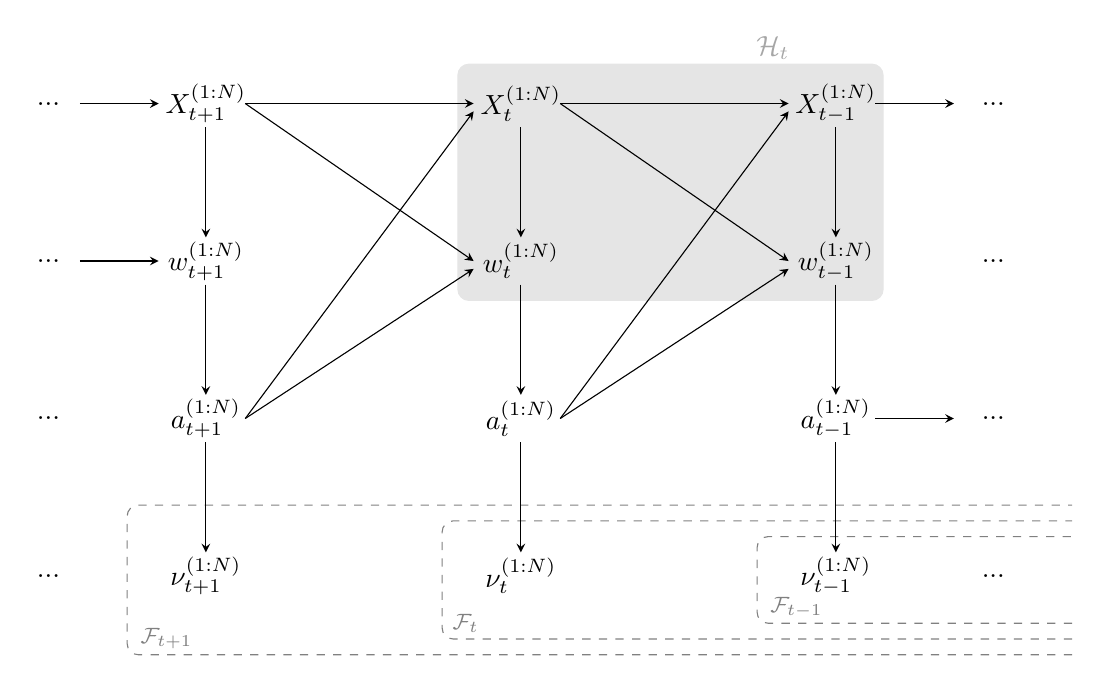
\begin{tikzpicture}[>=stealth]
% separatrix
\filldraw[gray!20, rounded corners] (3.2,0.5)--(8.6,0.5)--(8.6,-2.5)--(3.2,-2.5)--cycle;
\node[gray!70] at (7.2,0.7) {$\mathcal{H}_t$};
% left dots
\node at (-2,0) {...};
\node at (-2,-2) {...};
\node at (-2,-4) {...};
\node at (-2,-6) {...};
% labels (t+1)
\node at (0,0) {$X_{t+1}^{(1:N)}$};
\node at (0,-2) {$w_{t+1}^{(1:N)}$};
\node at (0,-4) {$a_{t+1}^{(1:N)}$};
\node at (0,-6) {$\nu_{t+1}^{(1:N)}$};
% labels t
\node at (4,0) {$X_{t}^{(1:N)}$};
\node at (4,-2) {$w_{t}^{(1:N)}$};
\node at (4,-4) {$a_{t}^{(1:N)}$};
\node at (4,-6) {$\nu_{t}^{(1:N)}$};
% labels (t-1)
\node at (8,0) {$X_{t-1}^{(1:N)}$};
\node at (8,-2) {$w_{t-1}^{(1:N)}$};
\node at (8,-4) {$a_{t-1}^{(1:N)}$};
\node at (8,-6) {$\nu_{t-1}^{(1:N)}$};
% right dots
\node at (10,0) {...};
\node at (10,-2) {...};
\node at (10,-4) {...};
\node at (10,-6) {...};
%filtrations
\draw [rounded corners, dashed, gray] (11,-6.6)--(7,-6.6)--(7,-5.5)--(11,-5.5);
\draw [rounded corners, dashed, gray] (11,-6.8)--(3,-6.8)--(3,-5.3)--(11,-5.3);
\draw [rounded corners, dashed, gray] (11,-7)--(-1,-7)--(-1,-5.1)--(11,-5.1);
% filtration labels
\node[gray] at (7.5,-6.4) {\footnotesize{$\mathcal{F}_{t-1}$}};
\node[gray] at (3.3,-6.6) {\footnotesize{$\mathcal{F}_{t}$}};
\node[gray] at (-0.5,-6.8) {\footnotesize{$\mathcal{F}_{t+1}$}};
% arrows (t+1) -> t
\draw[->] (0.5,0)--(3.4,0);
\draw[->] (0.5,0)--(3.4,-2);
\draw[->] (0.5,-4)--(3.4,-2.1);
\draw[->] (0.5,-4)--(3.4,-0.1);
% arrows t -> (t-1)
\draw[->] (4.5,0)--(7.4,0);
\draw[->] (4.5,0)--(7.4,-2);
\draw[->] (4.5,-4)--(7.4,-2.1);
\draw[->] (4.5,-4)--(7.4,-0.1);
% vertical arrows (t+1)
\draw[->] (0,-0.3)--(0,-1.7);
\draw[->] (0,-2.3)--(0,-3.7);
\draw[->] (0,-4.3)--(0,-5.7);
% vertical arrows t
\draw[->] (4,-0.3)--(4,-1.7);
\draw[->] (4,-2.3)--(4,-3.7);
\draw[->] (4,-4.3)--(4,-5.7);
% vertical arrows (t-1)
\draw[->] (8,-0.3)--(8,-1.7);
\draw[->] (8,-2.3)--(8,-3.7);
\draw[->] (8,-4.3)--(8,-5.7);
% arrows ... -> t+1
\draw[->] (-1.6,0)--(-0.6,0);
\draw[->] (-1.6,-2)--(-0.6,-2);
% arrows t-1 -> ...
\draw[->] (8.5,0)--(9.5,0);
\draw[->] (8.5,-4)--(9.5,-4);
\end{tikzpicture}
\caption[Construction of separatrix $\mathcal{H}_t$]{Part of the conditional dependence graph implied by Algorithm \ref{alg:SMC} illustrating the construction of $\mathcal{H}_t$. The direction of time is from left to right. The reverse-time filtration is indicated by the dashed areas. The nodes highlighted in grey generate the separatrix $\mathcal{H}_t$ between $a_t^{(1:N)}$ and $\mathcal{F}_{t-1}$.}
\label{fig:cond_indep_graph_Ht}
\end{figure}




\section{Multinomial resampling}
\label{sec:corol_mn}
Multinomial resampling is often preferred in theoretical studies of SMC, because it renders the parental indices conditionally i.i.d. given the weights, making it relatively simple to analyse the resulting algorithm.
The convergence of finite-dimensional distributions for multinomial resampling was proved in \textcite[Corollary 1]{koskela2018}, but we are now able to prove an analogous weak convergence result. The following proof also demonstrates the relative ease with which we can verify Theorem~\ref{thm:FDDconv} as opposed to \textcite[Theorem 1]{koskela2018}.
%The result of Corollary~\ref{thm:multinomial} was proved in \textcite[Corollary 1]{koskela2018}. It is also included here, firstly to demonstrate the relative ease with which it is proved under Theorem~\ref{thm:FDDconv} as opposed to \textcite[Theorem 1]{koskela2018}, and secondly to introduce the proof technique before proceeding to more complex resampling schemes.

\begin{corollary}\label{thm:multinomial}
Consider an SMC algorithm using multinomial resampling, such that \ref{standing_assumption} is satisfied. Assume there exist constants $\varepsilon\in (0,1], a\in [1,\infty)$ and probability density $h$ such that for all $x, x^\prime, t$,
\begin{equation}\label{eq:gq_bounds_mn}
\frac{1}{a} \leq g_t(x, x^\prime) \leq a , \quad
\varepsilon h(x^\prime) \leq q_t(x, x^\prime) \leq \frac{1}{\varepsilon} h(x^\prime) .
\end{equation}
Let $(G_t^{(n,N)})_{t\geq0}$ denote the genealogy of a random sample of $n$ terminal particles from the output of the algorithm among a total of $N$ particles. Then, for any fixed $n$, the time-scaled genealogy $(G_{\tau_N(t)}^{(n,N)})_{t\geq0}$ converges weakly to Kingman's $n$-coalescent as $N\to \infty$.%, in the sense of finite-dimensional distributions.
\end{corollary}
The bounds on $g_t$ and $q_t$ in \eqref{eq:gq_bounds_mn} are rather strong; they can only reasonably be expected to hold if the state space is compact. 
However, they are widespread in the literature, where they are known as the \emph{strong mixing conditions} \parencite[Section 3.5.2]{delmoral2004}, because they greatly facilitate the theoretical analysis of SMC algorithms. It is often possible to relax these conditions at the expense of considerable technical complication.
The conditions on $g_t$ in \eqref{eq:gq_bounds_mn} ensure that the weights are all $O(N^{-1})$, none of them being too close to zero or one. Together with the bounds on $q_t$, this is enough to control the relative rate of multiple mergers, as seen in the following proof.
%In the following proof, conditions \eqref{eq:gq_bounds_mn} ensure that the weights are all $O(N^{-1})$, none of them being too close to zero or one, which controls the relative rate of multiple mergers.

\begin{proof}
%Define the $\sigma$-algebras $\mathcal{H}_t$ as in \eqref{eq:defn_Ht}.
%Recall that the sequence of $\sigma$-algebras
%\begin{equation}%\label{eq:defn_Ht}
%\mathcal{H}_t := \sigma(X_{t-1}^{(1:N)}, X_t^{(1:N)}, w_{t-1}^{(1:N)}, w_t^{(1:N)} )
%\end{equation}
%are such that $\nu_t^{(1:N)}$ is conditionally independent of the filtration $\mathcal{F}_{t-1}$ given $\mathcal{H}_t$.
Define $\mathcal{H}_t$ as in \eqref{eq:defn_Ht}.
Conditional on $\mathcal{H}_t$ the parental indices are independent, with conditional law
\begin{equation}\label{eq:parentslaw_mn}
\Prob \left[ a_t^{(i)} = a_i \mid \mathcal{H}_t \right] 
%\propto w_t^{(a_i)} q_{t-1}(X_t^{(a_i)}, X_{t-1}^{(i)})
\propto g_t( X_{t+1}^{a_{t+1}^{(a_i)}} , X_t^{(a_i)} ) q_{t-1}(X_t^{(a_i)}, X_{t-1}^{(i)})
\end{equation}
for each $i$, so the joint law is
\begin{equation*}
\Prob \left[ a_t^{(1:N)} = a_{1:N} \mid \mathcal{H}_t \right] 
%\propto \prod_{i=1}^N w_t^{(a_i)} q_{t-1}(X_t^{(a_i)}, X_{t-1}^{(i)}).
\propto \prod_{i=1}^N g_t( X_{t+1}^{a_{t+1}^{(a_i)}} , X_t^{(a_i)} ) 
        q_{t-1}(X_t^{(a_i)}, X_{t-1}^{(i)}).
\end{equation*}
%
%%%%%%%%%
%
%The bounds on $g_t$ in \eqref{eq:gq_bounds_mn} imply 
%almost sure bounds on the weights
%%the almost sure bounds
%%\begin{equation*}
%%\frac{1}{a^2 N}
%%\leq w_t^{(i)}
%%\leq \frac{a^2}{N}
%%\end{equation*}
%which, along with the bounds on $q_{t-1}$ from \eqref{eq:gq_bounds_mn}, allows us to apply a balls-in-bins coupling presented in \textcite[Proof of Lemma 3]{koskela2018} to obtain bounds on expectations of functions of $a_t^{(1:N)}$.
Using the bounds \eqref{eq:gq_bounds_mn} and the balls-in-bins coupling of \textcite[Proof of Lemma 3]{koskela2018}, we can obtain bounds on expectations of functions of $a_t^{(1:N)}$.
For any $k\in\mathbb{N}$ the function $a_t^{(1:N)} \to (\nu_t^{(i)})_k$ is $\{i\}$-increasing in the sense of \textcite{koskela2018}, so we may apply the bounds
\begin{equation*}
\E[ (V_1^{(i)})_k ]
\leq \E[ (\nu_t^{(i)})_k \mid \mathcal{H}_t ]
\leq \E[ (V_2^{(i)})_k ] ,
\end{equation*}
where
\begin{align*}
& V_1^{(i)} 
\sim \Bin\left(N, \frac{\varepsilon/a}{(\varepsilon/a) + (N-1)(a/\varepsilon)} \right),\\
& V_2^{(i)} 
\sim \Bin\left( N, \frac{a/\varepsilon}{(a/\varepsilon) + (N-1)(\varepsilon/a)} \right) .
\end{align*}
independently for each $i$ and independently of $\mathcal{F}_\infty$.
Furthermore, using the moments of the Binomial distribution \parencite[see for example][p. 67]{mosimann1962}
\begin{equation*}
\E[ (V_1^{(i)})_k ]
= (N)_k \left( \frac{ \varepsilon/a }{ (\varepsilon/a) + (N-1)(a/\varepsilon) } \right)^k
\geq (N)_k \left( \frac{ \varepsilon/a }{ N(a/\varepsilon) } \right)^k
= \frac{(N)_k}{N^k} \frac{\varepsilon^{2k}}{a^{2k}} .
\end{equation*}
Similarly, 
\begin{equation*}
\E[ (V_2^{(i)})_k ]
\leq \frac{(N)_k}{N^k} \frac{a^{2k}}{\varepsilon^{2k}} .
\end{equation*}
We therefore have the bounds
\begin{equation*}
\frac{(N)_k}{N^k} \frac{\varepsilon^{2k}}{a^{2k}}
\leq \E[ (\nu_t^{(i)})_k \mid \mathcal{H}_t ]
\leq \frac{(N)_k}{N^k} \frac{a^{2k}}{\varepsilon^{2k}} . %\label{eq:mn_nuk_bounds}
\end{equation*}
for each $k$. Consequently,
\begin{equation}
\frac{1}{(N)_2} \sum_{i=1}^N \E[ (\nu_t^{(i)})_2 \mid \mathcal{H}_t ]
\geq \frac{\varepsilon^4}{Na^4} \label{eq:mn_cN_LB}
\end{equation}
and
\begin{equation}
\frac{1}{(N)_3} \sum_{i=1}^N \E[ (\nu_t^{(i)})_3 \mid \mathcal{H}_t ]
\leq \frac{a^6}{N^2 \varepsilon^6} . \label{eq:mn_cN3_UB}
\end{equation}
%
%%%%%%%%%
%
%\textcite{koskela2018} makes the following observation, which follows from a balls-in-bins coupling.
%Assume \eqref{eq:gq_bounds_mn}. 
%Then for any function $f:\{1,\dots,N\}^N \to \mathbb{R}$ such that (for a fixed $i$) $f(a_t^{\prime(1:N)}) \geq f(a_t^{(1:N)})$ whenever $|\{j:a_t^{\prime(j)}=i\}| \geq |\{j:a_t^{(j)}=i\}|$,
%\begin{equation}\label{eq:mn_f_bound}
%\E[ f(A_{1,i}^{(1:N)}) ] 
%\leq \E[ f(a_t^{(1:N)}) \mid \mathcal{H}_t ]
%\leq \E[ f(A_{2,i}^{(1:N)}) ] 
%\end{equation}
%where the elements of $A_{1,i}^{(1:N)}, A_{2,i}^{(1:N)}$ are all mutually independent and independent of $\mathcal{F}_{\infty}$, and distributed according to
%\begin{align*}
%& A_{1,i}^{(j)} 
%\sim \Cat \left( (\varepsilon/a)^{\1{i=1} -\1{i\neq 1}} ,
%        \dots, (\varepsilon/a)^{\1{i=N} -\1{i\neq N}} \right) \\
%& A_{2,i}^{(j)} 
%\sim \Cat \left( (a/\varepsilon)^{\1{i=1} -\1{i\neq 1}} ,
%        \dots, (a/\varepsilon)^{\1{i=N} -\1{i\neq N}} \right)
%\end{align*}
%independently for each $j$, where the vector of probabilities is given up to a constant in the argument of Categorical distributions.
%We will use these random vectors to construct bounds that are independent of $\mathcal{F}_\infty$.
%Also define the corresponding offspring counts $V_1^{(i)} = |\{j: A_{1,i}^{(j)}=i\}|$, $V_2^{(i)} = |\{j: A_{2,i}^{(j)}=i\}|$, for $i=1,\dots,N$, which have marginal distributions
%\begin{align*}
%& V_1^{(i)} 
%\sim \Bin\left(N, \frac{\varepsilon/a}{(\varepsilon/a) + (N-1)(a/\varepsilon)} \right),\\
%& V_2^{(i)} 
%\sim \Bin\left( N, \frac{a/\varepsilon}{(a/\varepsilon) + (N-1)(\varepsilon/a)} \right) .
%\end{align*}
%\seb{ Could state that a particular consequence of \eqref{eq:mn_f_bound} and $V_1,V_2$ etc.\ is
%\begin{equation*}
%\frac{(N)_k}{N^k} \frac{\varepsilon^{2k}}{a^{2k}}
%\leq \E[ (\nu_t^{(i)})_k \mid \mathcal{H}_t ]
%\leq \frac{(N)_k}{N^k} \frac{a^{2k}}{\varepsilon^{2k}} .
%\end{equation*}
%for any $k\in\mathbb{N}$? This is easily proved in much the same way as the two special cases below. This could probably replace \eqref{eq:mn_f_bound} and the surrounding argument, since all $f$s we use are of this particular form.}
%Now consider the function $f_i(a_t^{(1:N)}) := (\nu_t^{(i)})_2$. We can apply \eqref{eq:mn_f_bound} to obtain the lower bound
%\begin{align}
%\frac{1}{(N)_2} \sum_{i=1}^N \E[ (\nu_t^{(i)})_2 \mid \mathcal{H}_t ]
%&\geq \frac{1}{(N)_2} \sum_{i=1}^N \E[ (V_1^{(i)})_2 ]
%= \frac{1}{(N)_2} \sum_{i=1}^N (N)_2 \left[ \frac{ \varepsilon/a}{ (\varepsilon/a) + (N-1)(a/\varepsilon) } \right]^2 \notag\\
%&\geq \sum_{i=1}^N \left[ \frac{ \varepsilon/a}{ N a/\varepsilon } \right]^2
%= \frac{\varepsilon^4}{Na^4} \label{eq:mn_cN_LB}
%\end{align}
%using the moments of the Binomial distribution \parencite[see for example]{mosimann1962}.
%Similarly, we derive an upper bound on $f_i(a_t^{(1:N)}) := (\nu_t^{(i)})_3$:
%\begin{align}
%\frac{1}{(N)_3} \sum_{i=1}^N \E[ (\nu_t^{(i)})_3 \mid \mathcal{H}_t]
%&\leq \frac{1}{(N)_3} \left[ \sum_{i=1}^N \E[ (V_2^{(i)})_3 ] \right]
%= \frac{1}{(N)_3} \sum_{i=1}^N (N)_3 \left[ \frac{ a/\varepsilon }{ (a/\varepsilon) + (N-1)(\varepsilon/a) } \right]^3 \notag\\
%&\leq \sum_{i=1}^N \left[ \frac{ a/\varepsilon }{ N \varepsilon/a } \right]^3
%= \frac{a^6}{N^2\varepsilon^6} . \label{eq:mn_cN3_UB}
%\end{align}
%
%The definition of $\mathcal{H}_t$ is such that, for any suitable function $f$, by the tower property and conditional independence we have
%\begin{equation}
%\Et[ f(\nu_t^{(1:N)}) ] 
%= \Et\left[ \E[ f(\nu_t^{(1:N)}) \mid \mathcal{H}_t, \mathcal{F}_{t-1} ] \right] 
%= \Et\left[ \E[ f(\nu_t^{(1:N)}) \mid \mathcal{H}_t ] \right] .\label{eq:condexp_HtFt}
%\end{equation}
Applying \eqref{eq:condexp_HtFt} to \eqref{eq:mn_cN_LB} and \eqref{eq:mn_cN3_UB} we find
\begin{align*}
\frac{\frac{1}{(N)_3} \sum_{i=1}^N \Et[ (\nu_t^{(i)})_3 ]}{\frac{1}{(N)_2} \sum_{i=1}^N \Et[ (\nu_t^{(i)})_2 ]}
&\leq \frac{ a^6 / (N^2 \varepsilon^6) }{ \varepsilon^4 / (N a^4) }
= \frac{ a^{10} }{ N\varepsilon^{10} }
=: b_N \underset{N\to\infty}{\longrightarrow} 0.
\end{align*}
Thus \eqref{eq:mainthmcond} is satisfied. 
It remains to show that, for $N$ sufficiently large, $\Prob[ \tau_N(t) = \infty ] =0$ for all finite $t$, a technicality which is proved in Lemma \ref{thm:mn_nontriviality}. 
Applying Theorem~\ref{thm:weakconv} then yields the result.
\end{proof}



\begin{lemma}\label{thm:mn_nontriviality}
Consider an SMC algorithm using multinomial resampling, satisfying \ref{standing_assumption} and \eqref{eq:gq_bounds_mn}. 
Then, for all $N>2$, $\Prob[ \tau_N(t) = \infty ]=0$ for all finite $t$.
\end{lemma}

\begin{proof}
Since $c_N(t) \in [0,1]$ almost surely and has strictly positive expectation, for any fixed $N$ the distribution of $c_N(t)$ with given expectation that maximises $\Prob[ c_N(t)=0 \mid \mathcal{F}_{t-1} ]$ is two atoms, at 0 and 1 respectively. To ensure the correct expectation, the atom at 1 should have mass $\Prob[ c_N(t)=1 \mid \mathcal{F}_{t-1} ] = \Et [ c_N(t) ]$, which is bounded below by \eqref{eq:mn_cN_LB}.
If $c_N(t) > 0$ then $c_N(t) \geq 2/(N)_2 > 2/N^2$. Hence, in general $\Prob[ c_N(t) > 2/N^2 \mid \mathcal{F}_{t-1} ] \geq \Et [c_N(t)]$. 
Applying \eqref{eq:mn_cN_LB} along with \eqref{eq:condexp_HtFt}, we have for any finite $N$
\begin{equation*}
\sum_{t=0}^\infty \Prob[ c_N(t) > 2/N^2 \mid \mathcal{F}_{t-1} ]
\geq \sum_{t=0}^\infty \Et [ c_N(t) ]
\geq \sum_{t=0}^\infty \frac{\varepsilon^4}{Na^4}
= \infty .
\end{equation*}
By a filtered version of the second Borel--Cantelli lemma \parencite[see for example][Theorem 4.3.4]{durrett2019}, this implies that $c_N(t) >2/N^2$ for infinitely many $t$, almost surely.
This ensures, for all $t <\infty$, that $\Prob\left[ \exists s<\infty : \sum_{r=1}^s c_N(r) \geq t \right] =1$, which by definition of $\tau_N(t)$ is equivalent to $\Prob[ \tau_N(t) = \infty ] =0$.
\end{proof}




\section{Stratified resampling}

\begin{corollary}\label{thm:stratified}
Consider an SMC algorithm using stratified resampling, such that \ref{standing_assumption} is satisfied.
Assume that there exists a constant $a\in [1,\infty)$ such that for all $x, x^\prime, t$,
\begin{equation}\label{eq:gq_bounds_sr}
\frac{1}{a} \leq g_t(x, x^\prime) \leq a .
\end{equation}
Assume that $\Prob[ \tau_N(t) = \infty] =0$ for all finite $t$.
Let $(G_t^{(n,N)})_{t\geq0}$ denote the genealogy of a random sample of $n$ terminal particles from the output of the algorithm among a total of $N$ particles. Then, for any fixed $n$, the time-scaled genealogy $(G_{\tau_N(t)}^{(n,N)})_{t\geq0}$ converges weakly to Kingman's $n$-coalescent as $N\to \infty$.%, in the sense of finite-dimensional distributions.
\end{corollary}
Stratified resampling is, by design, much more restrictive than multinomial resampling. Once the weights are known there is little freedom in the offspring counts, so it is not surprising that control over the weights such as \eqref{eq:gq_bounds_sr} provides is sufficient without any additional control over the transition densities $q_t$. 
Indeed the transition kernels need not even admit densities.
This is in contrast to multinomial resampling (Corollary~\ref{thm:multinomial}), where $g_t$ and $q_t$ are more or less on an equal footing, and we require both to be bounded.

It is not immediately clear that the finite time scale condition $\Prob[ \tau_N(t) = \infty] =0$ holds under conditions \eqref{eq:gq_bounds_sr}, so it is included in the statement of the corollary. Proposition~\ref{thm:SR_nontriviality} presents some sufficient conditions for the finite time scale, but these are by no means necessary.

\begin{proof}
Define the $\sigma$-algebras $\mathcal{H}_t$ as in \eqref{eq:defn_Ht}.
With stratified resampling, conditional on the weights each offspring count almost surely takes one of four values: $\nu_t^{(i)} \in \{ \flnw -1, \flnw, \flnw +1, \flnw +2 \}$.  
Define for each $k\in\mathbb{Z}$
\begin{equation}\label{eq:pk_defn}
p_k^{(i)} := \Prob \left[ \nu_t^{(i)} = \flnw + k \midd \mathcal{H}_t \right] .
\end{equation}
Then $p_k^{(i)} \equiv 0$ for $k\notin \{-1,0,1,2\}$.
%Denote $p_j^{(i)} := \Prob[ \nu_t^{(i)} = \flnw +j \mid \mathcal{H}_t ]$ for $j=-1,0,1,2$.
Now
\begin{align*}
\E [(\nu_t^{(i)})_2 \mid \mathcal{H}_t ]
&= p_{-1}^{(i)} (\flnw -1)_2 + p_0^{(i)} (\flnw)_2 + p_1^{(i)} (\flnw +1)_2 \\
    &\hspace{3cm} + p_2^{(i)} (\flnw +2)_2
\end{align*}
and
\begin{align}
\E [(\nu_t^{(i)})_3 \mid \mathcal{H}_t ]
&= p_{-1}^{(i)} (\flnw -1)_3 + p_0^{(i)} (\flnw)_3 + p_1^{(i)} (\flnw +1)_3 \notag\\
    &\hspace{1cm} + p_2^{(i)} (\flnw +2)_3 \notag\\
&= p_{-1}^{(i)} (\flnw -3)(\flnw -1)_2 + p_0^{(i)} (\flnw -2)(\flnw)_2 \notag\\
     &\hspace{1cm} + p_1^{(i)} (\flnw -1)(\flnw +1)_2 
         + p_2^{(i)} \flnw (\flnw +2)_2 \notag\\
&\leq \flnw \Big\{ p_{-1}^{(i)} (\flnw -1)_2 + p_0^{(i)} (\flnw)_2 
        + p_1^{(i)} (\flnw +1)_2 \notag\\
    &\hspace{1cm} + p_2^{(i)} (\flnw +2)_2 \Big\} \notag\\
&= \flnw ]\E [(\nu_t^{(i)})_2 \mid \mathcal{H}_t ] \notag\\
&\leq a^2 \E [(\nu_t^{(i)})_2 \mid \mathcal{H}_t ] . \label{eq:strat_v2_versus_v3}
\end{align}
The last line uses the almost sure bound $w_t^{(i)} \leq a^2 /N$ which follows from \eqref{eq:gq_bounds_sr} along with the form of the weights in Algorithm \ref{alg:SMC}.
Note that some terms in the above expressions may be equal to zero when $w_t^{(i)}$ is small enough, but the bound still holds in these cases.
Since \eqref{eq:strat_v2_versus_v3} holds for all $i$, applying the tower rule we have
\begin{equation*}
\frac{1}{(N)_3} \sum_{i=1}^{N} \Et [(\nu_t^{(i)})_3 ]
\leq \frac{a^2}{N-2} \frac{1}{(N)_2} \sum_{i=1}^{N} \Et [(\nu_t^{(i)})_2 ] ,
\end{equation*}
satisfying \eqref{eq:mainthmcond} with $b_N := a^2/(N-2) \rightarrow 0$.
The result follows by applying Theorem~\ref{thm:weakconv}.
\end{proof}



\begin{prop}\label{thm:strat_nontriviality}
Consider an SMC algorithm using stratified resampling.
Suppose that there exists a constant $\varepsilon \in (0,1]$ and a probability density $h$ such that
\begin{equation*}
\varepsilon h(x') \leq q_t(x, x^\prime) \leq \varepsilon^{-1} h(x')
\end{equation*}
uniformly in $x,t$, and that there exist $\zeta >0$ and $\delta \in (0,1)$ such that 
\begin{equation}
\Prob[ \max_i w_t^{(i)} - \min_i w_t^{(i)} \geq 2\delta/N \mid \mathcal{F}_{t-1} ] \geq \zeta \label{eq:strat_minmaxweight}
\end{equation}
 for infinitely many $t$. Then, for all $N>1$, $\Prob[ \tau_N(t) = \infty ] =0$ for all finite $t$.
\end{prop}
We now assume $q_t$ is bounded above and away from zero, as in \eqref{eq:gq_bounds_mn}.
We saw that such a condition was not necessary for Corollary~\ref{thm:stratified}, and we do not believe it to be necessary here either; it is merely a convenient way to control the contributions from the transition density. Indeed, the terms in $\varepsilon$ appearing in the bounds established in the following proof are rather crude.
In fact, the stated condition is rather stronger than necessary: we only need the bounds on $q_t$ to hold for infinitely many $t$, rather than for all $t$. We use this stronger statement to avoid complicating the proof.
%The bounds established in the following proof are rather crude, particularly the terms in $\varepsilon$, so it may well be possible to achieve similar bounds under even less restrictive conditions on $q_t$.

The second condition \eqref{eq:strat_minmaxweight} is required to ensure that, at least infinitely often, the weights are not equal to $(1,\dots,1)/N$, since stratified resampling is degenerate under equal weights, which could cause the time scale to explode. 
It is hardly conceivable that any real SMC algorithm would fail to satisfy this very mild condition, which effectively ensures that the weights cannot be ``too well-behaved''.


\begin{proof}
As argued in Lemma~\ref{thm:mn_nontriviality}, it is sufficient to prove that under the stated conditions
\begin{equation*}
\sum_{r=0}^\infty \Prob[ c_N(r) > 2/N^2  \mid \mathcal{F}_{r-1} ] = \infty .
\end{equation*}
Firstly,
\begin{align}
\Prob[ c_N(t) \leq 2/N^2 \mid \mathcal{H}_t ]
&= \Prob[ c_N(t) =0 \mid \mathcal{H}_t ]
= \Prob[ \nu_t^{(i)} =1 \,\forall i\in\{1,\dots,N\} \mid \mathcal{H}_t ] \notag\\
&\leq \Prob[ \nu_t^{(i^\star)} =1 \mid \mathcal{H}_t ] , \label{eq:cNnonzero}
\end{align}
where $i^\star := \argmax_i \{ w_t^{(i)} \}$ (but note that the inequality holds when $i^\star$ is taken to be any particular index).
Define $p_k^{(i)}$ as in \eqref{eq:pk_defn} and recall that, under stratified resampling, $p_k^{(i)} \equiv 0$ for $k\notin \{-1,0,1,2\}$ and
\begin{equation*}
\sum_{k=-1}^2 p_k^{(i)} 
= \sum_{k=-1}^2 \Prob \left[ \nu_t^{(i)} = \flnw + k \midd w_t^{(1:N)} \right]
= 1 .
\end{equation*}
Up to a proportionality constant $C$,
\begin{align*}
p_k^{(i)} 
&= C \, \Prob \left[ \nu_t^{(i)} = \flnw + k \midd w_t^{(1:N)} \right] \\
    &\qquad \times \sum_{\substack{a_{1:N} \in \{1,\dots,N\}^N : 
        \\ |\{j: a_j=i\}|=\flnw +k }}
        \Prob\left[ a_t^{(1:N)} = a_{1:N} \midd \nu_t^{(i)}, w_t^{(1:N)} \right]
        \prod_{j=1}^N q_{t-1}( X_t^{(a_j)}, X_{t-1}^{(j)} ) 
\end{align*}
for each $k\in\{-1,0,1,2\}$.
We can bound each probability above and below using the almost sure bounds on $q_{t-1}$ from the statement of the Proposition (once the bounds on $q_{t-1}$ are brought outside, the remaining sum of probabilities is equal to one):
\begin{align*}
p_k^{(i)}
&\geq C \, \Prob \left[ \nu_t^{(i)} = \flnw + k \midd w_t^{(1:N)} \right] \varepsilon^N
        \prod_{j=1}^N h(X_{t-1}^{(j)}) , \\
p_k^{(i)}
&\leq C \, \Prob \left[ \nu_t^{(i)} = \flnw + k \midd w_t^{(1:N)} \right] 
        \varepsilon^{-N} \prod_{j=1}^N h(X_{t-1}^{(j)}) .
\end{align*}
We then eliminate the proportionality constant $C$ by normalising, to obtain lower bounds
\begin{align}
p_k^{(i)} 
&\geq \frac{ C \, \Prob [ \nu_t^{(i)} = \flnw + k \mid w_t^{(1:N)} ] 
        \varepsilon^N \prod_{j=1}^N h(X_{t-1}^{(j)}) }{
        \sum_{j=-1}^2 C \, \Prob [ \nu_t^{(i)} = \flnw + j \mid w_t^{(1:N)} ] 
        \varepsilon^{-N} \prod_{j=1}^N h(X_{t-1}^{(j)}) } \notag\\
%&= \frac{ \Prob [ \nu_t^{(i)} = \flnw + k \mid w_t^{(1:N)} ] \varepsilon^N }{
%        \varepsilon^{-N} } \notag\\
&= \Prob [ \nu_t^{(i)} = \flnw + k \mid w_t^{(1:N)} ] \varepsilon^{2N} 
        \label{eq:strat_pbounds}
\end{align}
for each $k$, which also imply
\begin{equation}
1 - p_k^{(i)} 
\geq \left( 1- \Prob [ \nu_t^{(i)} = \flnw + k \mid w_t^{(1:N)} ] \right)
        \varepsilon^{2N} . \label{eq:strat_nonpbounds}
\end{equation}

%Suppose that $\max_i w_t^{(i)} - \min_i w_t^{(i)} \geq 2\delta/N$. Then that at least one of $\{ \max_i w_t^{(i)} \geq (1+\delta)/N \}$ and $\{ \min_i w_t^{(i)} \leq (1-\delta)/N \}$ occurs. We will now examine each of these possibilities.
%
%We can always write the maximum weight as $w_t^{(i^\star)} = \frac{1+\delta^\prime}{N}$ for some $\delta^\prime \geq 0$. Then, using \eqref{eq:cNnonzero},
%\begin{equation*}
%\Prob[ c_N(t) > 2/N^2 \mid \mathcal{H}_t ]
%\geq 1- \Prob[ \nu_t^{(i^\star)} =1 \mid \mathcal{H}_t ]
%= \begin{cases}
%    1 - p_0^{(i^\star)} & \text{if } \delta^\prime \in [0,1) \\
%    1 - p_{-1}^{(i^\star)} & \text{if } \delta^\prime \in [1,2) \\
%    1 & \text{if } \delta^\prime \geq 2 .
%\end{cases}
%\end{equation*}
%If $\delta^\prime \in [0,1)$ then
%\begin{equation*}
%1 - p_0^{(i^\star)}
%= p_{-1}^{(i^\star)} + p_1^{(i^\star)} + p_2^{(i^\star)}
%\geq \left( 0 + \frac{\delta^\prime}{2} + 0 \right) \varepsilon^{2N} 
%= \frac{\delta^\prime \varepsilon^{2N} }{2}
%\end{equation*}
%using \eqref{eq:strat_pbounds} and the lower bounds in Table~\ref{tab:strat_probs}.
%Similarly, if $\delta^\prime \in [1,2)$ then
%\begin{equation*}
%1 - p_{-1}^{(i^\star)}
%= p_0^{(i^\star)} + p_1^{(i^\star)} + p_2^{(i^\star)}
%\geq \left( \frac{(1-\delta^\prime)^2}{2} + \frac{\delta^\prime}{2} + 0 \right)
%        \varepsilon^{2N} 
%\geq \frac{\delta^\prime \varepsilon^{2N} }{2} .
%\end{equation*}
%So overall, under the constraint $\max_i w_t^{(i)} \geq (1+\delta)/N$, we have
%\begin{equation*}
%\Prob[ c_N(t) > 2/N^2 \mid \mathcal{H}_t ]
%\geq \min_{\delta^\prime \geq \delta} 
%        \left\{ \frac{\delta^\prime \varepsilon^{2N} }{2} \right\}
%= \frac{ \delta \varepsilon^{2N} }{2} .
%\end{equation*}
%
%Now we construct a similar argument for the minimum weight. Let $j^\star := \argmin_i \{ w_t^{(i)} \}$ and write
%$w_t^{(j^\star)} = \frac{1-\delta^\prime}{N}$, for some $\delta^\prime \in [0,1]$.
%Then we have
%\begin{equation*}
%\Prob[ c_N(t) > 2/N^2 \mid \mathcal{H}_t ]
%\geq 1- \Prob[ \nu_t^{(i^\star)} =1 \mid \mathcal{H}_t ]
%=\begin{cases}
%    1- p_1^{(j^\star)} & \text{if } \delta^\prime \in (0,1] \\
%    0 & \text{if } \delta^\prime =0 .
%\end{cases}
%\end{equation*}
%If $\delta^\prime \in (0,1]$ then
%\begin{equation*}
%1- p_1^{(j^\star)} = p_{-1}^{(j^\star)} + p_0^{(j^\star)} + p_2^{(j^\star)}
%\geq \left( 0 + \frac{ (\delta^\prime)^2 }{2} + 0 \right) \varepsilon^{2N}
%= \frac{ (\delta^\prime)^2 \varepsilon^{2N} }{2} ,
%\end{equation*}
%again using the lower bounds in Table~\ref{tab:strat_probs}.
%Therefore, under the constraint $\min_i w_t^{(i)} \leq (1-\delta)/N$, we have
%\begin{equation*}
%\Prob[ c_N(t) > 2/N^2 \mid \mathcal{H}_t ]
%\geq \min_{\delta^\prime \geq \delta} 
%        \left\{ \frac{ (\delta^\prime)^2 \varepsilon^{2N} }{2} 
%        \I{\delta^\prime \neq 0} \right\}
%= \frac{ \delta^2 \varepsilon^{2N} }{2} .
%\end{equation*}
%Combining both cases, we find for arbitrary $r$
%\begin{equation*}
%\Prob[ c_N(r) > 2/N^2 \mid \mathcal{H}_r ] 
%\geq  \frac{ \delta^2 \varepsilon^{2N} }{2}
%        \I{ \max_i w_r^{(i)} - \min_i w_r^{(i)} \geq 2\delta/N }
%\end{equation*}
%so
%\begin{align*}
%\Prob[ c_N(r) > 2/N^2 \mid \mathcal{F}_{r-1} ] 
%&\geq  \frac{ \delta^2 \varepsilon^{2N} }{2}
%        \Prob[ \max_i w_r^{(i)} - \min_i w_r^{(i)} \geq 2\delta/N 
%        \mid \mathcal{F}_{r-1} ] \\
%&\geq \zeta \frac{ \delta^2 \varepsilon^{2N} }{2}
%> 0
%\end{align*}
%for infinitely many $r$.
%Hence
%\begin{equation*}
%\sum_{r=0}^\infty \Prob[ c_N(r) > 2/N^2  \mid \mathcal{F}_{r-1} ] = \infty
%\end{equation*}
%as required.

Suppose that $\max_i w_t^{(i)} - \min_i w_t^{(i)} \geq 2\delta/N$. Then that at least one of $\{ \max_i w_t^{(i)} \geq (1+\delta)/N \}$ and $\{ \min_i w_t^{(i)} \leq (1-\delta)/N \}$ occurs. We will now examine each of these possibilities.

We can always write the maximum weight as $w_t^{(i^\star)} = \frac{1+\gamma}{N}$ for some $\gamma \geq 0$. Then, using \eqref{eq:cNnonzero},
\begin{equation*}
\Prob[ c_N(t) > 2/N^2 \mid \mathcal{H}_t ]
\geq 1- \Prob[ \nu_t^{(i^\star)} =1 \mid \mathcal{H}_t ]
= \begin{cases}
    0 & \text{if } \gamma = 0 \\
    1 - p_0^{(i^\star)} & \text{if } \gamma \in (0,1) \\
    1 - p_{-1}^{(i^\star)} & \text{if } \gamma \in [1,2) \\
    1 & \text{if } \gamma \geq 2 .
\end{cases}
\end{equation*}
If $\gamma \in (0,1)$ then the ``overhang'' in the sense of Figure~\ref{fig:strat_cases} is $\gamma$, and
\begin{equation*}
1 - p_0^{(i^\star)}
%\geq 1 - \left( 1- \frac{3\delta^\prime}{4} \right) \varepsilon^{2N} 
\geq \frac{3\gamma }{4} \varepsilon^{2N}
\end{equation*}
using Table~\ref{tab:strat_probs} (upper bound on $p_0$) and \eqref{eq:strat_nonpbounds}.
Similarly, if $\gamma \in [1,2)$ then the overhang is $\gamma-1$ and by Table~\ref{tab:strat_probs} (upper bound on $p_{-1}$),
\begin{equation*}
1 - p_{-1}^{(i^\star)}
\geq \left( 1- \frac{1}{4} \right)
        \varepsilon^{2N} 
\geq \frac{3}{4} \varepsilon^{2N} .
\end{equation*}
Overall, under the constraint $\max_i w_t^{(i)} \geq (1+\delta)/N$, we have
\begin{equation*}
\Prob[ c_N(t) > 2/N^2 \mid \mathcal{H}_t ]
\geq \min_{\gamma \geq \delta} 
        \left\{ \frac{3\gamma }{4} \varepsilon^{2N} \I{\gamma \in [0,1)}
        + \frac{3 }{4} \varepsilon^{2N} \I{\gamma \in [1,2)}
        + \I{\gamma \geq 2} \right\}
= \frac{3}{4} \delta \varepsilon^{2N} .
\end{equation*}

We now construct a similar argument for the minimum weight. Let $j^\star := \argmin_i \{ w_t^{(i)} \}$ and write
$w_t^{(j^\star)} = \frac{1-\gamma}{N}$, for some $\gamma \in [0,1]$.
Then by \eqref{eq:cNnonzero} we have
\begin{equation*}
\Prob[ c_N(t) > 2/N^2 \mid \mathcal{H}_t ]
\geq 1- \Prob[ \nu_t^{(j^\star)} =1 \mid \mathcal{H}_t ]
=\begin{cases}
    1- p_1^{(j^\star)} & \text{if } \gamma \in (0,1] \\
    0 & \text{if } \gamma =0 .
\end{cases}
\end{equation*}
If $\gamma \in (0,1]$ then the ``overhang'' in the sense of Figure~\ref{fig:strat_cases} is $1-\gamma$, and
\begin{equation*}
1- p_1^{(j^\star)}
\geq \left( 1- \frac{1+ (1-\gamma)}{2} \right) \varepsilon^{2N}
= \frac{ \gamma }{2} \varepsilon^{2N} ,
\end{equation*}
using Table~\ref{tab:strat_probs} (upper bound on $p_1$).
Therefore, under the constraint $\min_i w_t^{(i)} \leq (1-\delta)/N$, we have
\begin{equation*}
\Prob[ c_N(t) > 2/N^2 \mid \mathcal{H}_t ]
\geq \min_{\gamma \geq \delta} 
        \left\{ \frac{ \gamma }{2} \varepsilon^{2N}
        %\I{\gamma \neq 0}
        \right\}
= \frac{1}{2} \delta \varepsilon^{2N} .
\end{equation*}
Combining both cases, we find for arbitrary $r$
\begin{equation*}
\Prob[ c_N(r) > 2/N^2 \mid \mathcal{H}_r ] 
\geq  \frac{1}{2} \delta \varepsilon^{2N} 
        \I{ \max_i w_r^{(i)} - \min_i w_r^{(i)} \geq 2\delta/N }
\end{equation*}
so, by the tower rule and conditional independence,
\begin{align*}
\Prob[ c_N(r) > 2/N^2 \mid \mathcal{F}_{r-1} ] 
&= \E_r \left[ \Prob[ c_N(r) > 2/N^2 \mid \mathcal{H}_r ] \right] \\
&\geq  \frac{1}{2} \delta \varepsilon^{2N} 
        \Prob[ \max_i w_r^{(i)} - \min_i w_r^{(i)} \geq 2\delta/N 
        \mid \mathcal{F}_{r-1} ] \\
&\geq \frac{1}{2} \delta \varepsilon^{2N} \zeta
> 0
\end{align*}
for infinitely many $r$.
Hence
\begin{equation*}
\sum_{r=0}^\infty \Prob[ c_N(r) > 2/N^2  \mid \mathcal{F}_{r-1} ] = \infty
\end{equation*}
as required.
\end{proof}



\section{Stochastic rounding}

\begin{corollary}\label{thm:stochrounding}
Consider an SMC algorithm using any stochastic rounding as its resampling scheme, such that \ref{standing_assumption} is satisfied.
Assume that there exists a constant $a\in [1,\infty)$ such that for all $x, x^\prime, t$,
\begin{equation*}
\frac{1}{a} \leq g_t(x, x^\prime) \leq a . 
\end{equation*}
Assume that $\Prob[ \tau_N(t) = \infty] =0$ for all finite $t$.
Let $(G_t^{(n,N)})_{t\geq0}$ denote the genealogy of a random sample of $n$ terminal particles from the output of the algorithm among a total of $N$ particles. Then, for any fixed $n$, the time-scaled genealogy $(G_{\tau_N(t)}^{(n,N)})_{t\geq0}$ converges weakly to Kingman's $n$-coalescent as $N\to \infty$.%, in the sense of finite-dimensional distributions.
\end{corollary}

\begin{proof}
We can apply exactly the proof of Corollary~\ref{thm:stratified}, except that stochastic rounding is more restrictive than stratified resampling, so that conditional on $w_t^{(1:N)}$ the only possible offspring counts (almost surely) are $\nu_t^{(i)} \in \{ \flnw, \flnw +1 \}$. We simply set $p_{-1}^{(i)} = p_{2}^{(i)} = 0$ in the proof of Corollary~\ref{thm:stratified} to see that
\begin{equation*}
\frac{1}{(N)_3} \sum_{i=1}^{N} \Et [(\nu_t^{(i)})_3 ]
\leq \frac{a^2}{N-2} \frac{1}{(N)_2} \sum_{i=1}^{N} \Et [(\nu_t^{(i)})_2 ]
\end{equation*}
as required.
The result then follows by applying Theorem~\ref{thm:weakconv}.
\end{proof}
We can also show, under additional conditions, that the assumption $\Prob[ \tau_N(t) = \infty ] =0$ for all finite $t$ holds.

\begin{prop}\label{thm:SR_nontriviality}
Consider an SMC algorithm using any stochastic rounding as its resampling scheme.
Suppose that there exists a constant $\varepsilon \in (0,1]$ and a probability density $h$ such that
\begin{equation*}
\varepsilon h(x') \leq q_t(x, x^\prime) \leq \varepsilon^{-1} h(x')
\end{equation*}
uniformly in $x,t$, and that there exist $\zeta >0$ and $\delta \in (0,1)$ such that 
\begin{equation*}
\Prob[ \max_i w_t^{(i)} - \min_i w_t^{(i)} \geq 2\delta/N \mid \mathcal{F}_{t-1} ] \geq \zeta
\end{equation*}
 for infinitely many $t$. Then, for all $N>1$, $\Prob[ \tau_N(t) = \infty ] =0$ for all finite $t$.
\end{prop}
This result was published in \textcite[Lemma B.1]{brown2021} with the slightly stronger conditions where the bounds on $q_t$ are also uniform in $x^\prime$. It has since been noted that the conditions given here are sufficient; the $h$ terms can be  cancelled as in \eqref{eq:strat_pbounds}.
As was the case for Proposition~\ref{thm:strat_nontriviality}, for convenience the conditions on $q_t$ are made stronger than necessary.

%\seb{If I find a more elegant proof for e.g. stratified, I can use the techniques to simplify this one a bit too.}
%
%\begin{proof}[Proof version 1]
%Let $\mathcal{H}_t$ be defined as in \eqref{eq:defn_Ht}. The first step is to show that whenever $\max_i w_t^{(i)} \geq (1+\delta)/N$, $\Prob[  c_N(t) > 2/N^2 \mid \mathcal{H}_t ] = \Prob[ c_N(t) \neq 0 \mid \mathcal{H}_t ]$ is bounded below uniformly in $t$.
%For this purpose we need consider only weight vectors such that $w_t^{(i)} \in (0,2/N)$ for all $i$; otherwise $\Prob[ c_N(t) \neq 0 \mid \mathcal{H}_t ] =1$ by the definition of stochastic rounding.
%
%Denote $\mathcal{S}_{N-1}^\delta = \{ w^{(1:N)} \in \mathcal{S}_{N-1} :  \forall i, \, 0 <w^{(i)} <2/N ;\, \max_i w^{(i)} \geq (1 + \delta)/N \}$ for any $\delta \in (0, 1)$, where $\mathcal{S}_{k}$ denotes the $k$-dimensional probability simplex.
%Fix arbitrary $w_t^{(1:N)} \in \mathcal{S}_{N-1}^\delta$. Set $i^\star = \arg\max_i w_t^{(i)}$ and denote $\mathcal{I} = \{i \in \{1,\dots,N\} : w^{(i)} > 1/N \}$.
%Since all weights are in $(0, 2/N)$, for $i \in \mathcal{I}, \nu_t^{(i)} \in \{1,2\}$ and for $i \notin \mathcal{I}, \nu_t^{(i)} \in \{0,1\}$; and since the offspring counts must sum to $N$, we can write
%\begin{align}\label{eq:smallcN_istar}
%\Prob[ c_N(t) \leq 2/N^2 \mid \mathcal{H}_t ]
%&= \Prob[ \nu_t^{(i)} =1 \,\forall i\in\{1,\dots,N\} \mid \mathcal{H}_t ] \notag\\
%&= \Prob[ \nu_t^{(i)} =1 \,\forall i\in \mathcal{I} \mid \mathcal{H}_t ] \notag\\
%&= \prod_{i \in \mathcal{I}} \Prob[ \nu_t^{(i)} =1 \mid \nu_t^{(j)}=1 \,\forall j \in \mathcal{I}: j<i; \mathcal{H}_t ] \notag\\
%&= \Prob[ \nu_t^{(i^\star)} =1 \mid \mathcal{H}_t ] \prod_{\substack{i \in \mathcal{I} \\ i \neq i^\star}} \Prob[ \nu_t^{(i)} =1 \mid \nu_t^{(i^\star)}=1; \nu_t^{(j)}=1 \,\forall j \in \mathcal{I}: j<i ; \mathcal{H}_t ] \notag\\
%&\leq \Prob[ \nu_t^{(i^\star)} =1 \mid \mathcal{H}_t ] .
%\end{align}
%The final inequality holds with equality when $|\mathcal{I}| =1$, i.e.\ the only weight larger than $1/N$ is $w_t^{(i^\star)}$.
%Thus $\Prob[ c_N(t) > 2/N^2 \mid \mathcal{H}_t ]$ is minimised on $\mathcal{S}_{N-1}^\delta$ when only one weight is larger than $1/N$, in which case the values of the other weights do not affect this probability. 
%
%Define $w_{\delta^\prime} = \{(1,\dots,1) + \delta^\prime e_{i^\star} - \delta^\prime e_{j^\star} \} /N$ for fixed $i^\star \neq j^\star$ and $\delta^\prime \in (0,1)$, where $e_i$ denotes the $i$th canonical basis vector in $\mathbb{R}^N$. 
%As in the proof of Corollary~\ref{thm:stochrounding}, define $p_0^{(i)} = \Prob[ \nu_t^{(i)} = \flnw \mid \mathcal{H}_t ]$ and $p_1^{(i)} = \Prob[ \nu_t^{(i)} = \flnw +1 \mid \mathcal{H}_t ]$. Then from \eqref{eq:smallcN_istar} we have
%\begin{equation*}
%\Prob[ c_N(t) > 2/N^2 \mid \mathcal{H}_t, w_t^{(1:N)} = w_{\delta^\prime} ]
%= 1- \Prob[ \nu_t^{(i^\star)} = 1 \mid \mathcal{H}_t, w_t^{(1:N)} = w_{\delta^\prime} ]
%= p_1^{(i^\star)},
%\end{equation*}
%evaluated on $w_{\delta^\prime}$.
%We will need a lower bound on $p_1^{(i^\star)}$ when $w_t^{(1:N)} = w_{\delta^\prime}$. 
%We first derive expressions for $p_0^{(i)}$ and $p_1^{(i)}$ up to a constant, then use $p_0^{(i)} + p_1^{(i)} =1$ to get a normalised bound. We have
%\begin{align*} 
%p_0^{(i)} &= C (1- N w_t^{(i)} + \flnw) \\
%&\qquad \times \sum_{\substack{a_{1:N} \in \{1,\dots,N\}^N : \\ |\{j: a_j=i\}|=\flnw }}
%\Prob\left[ a_t^{(1:N)} = a_{1:N} \mid \nu_t^{(i)}, w_t^{(1:N)} \right]
%\prod_{k=1}^N q_{t-1}( X_t^{(a_k)}, X_{t-1}^{(k)} ) ,\\
%p_1^{(i)} &= C (N w_t^{(i)} - \flnw) \\
%&\qquad \times \sum_{\substack{a_{1:N} \in \{1,\dots,N\}^N : \\ |\{j: a_j=i\}|=\flnw +1 }}
%\Prob\left[ a_t^{(1:N)} = a_{1:N} \mid \nu_t^{(i)}, w_t^{(1:N)} \right]
%\prod_{k=1}^N q_{t-1}( X_t^{(a_k)}, X_{t-1}^{(k)} ) .
%\end{align*}
%Applying the bounds on $q_t$, we have
%\begin{align*}
%C (1- N w_t^{(i)} + \flnw) \varepsilon^N &\leq p_0^{(i)} \leq C (1- N w_t^{(i)} + \flnw) \varepsilon^{-N} ,\\
%C (N w_t^{(i)} - \flnw) \varepsilon^N &\leq p_1^{(i)} \leq C (N w_t^{(i)} - \flnw) \varepsilon^{-N}
%\end{align*}
%from which we construct the normalised bound
%\begin{equation*}
%p_1^{(i)} \geq \frac{ (Nw_t^{(i)} - \flnw) \varepsilon^{N} }{ (Nw_t^{(i)} - \flnw) \varepsilon^{-N} + (1- Nw_t^{(i)} +\flnw) \varepsilon^{-N}}
%= (Nw_t^{(i)} - \flnw) \varepsilon^{2N} .
%\end{equation*}
%When $w_t^{(1:N)} = w_{\delta^\prime}$, we have $w_t^{(i^\star)} = (1+\delta^\prime)/N$, so $p_1^{(i^\star)} \geq \delta^\prime \varepsilon^{2N}$,
%which is increasing in $\delta^\prime$.
%We conclude that $\Prob[ c_N(t) > 2/N^2 | \mathcal{H}_t, \max_i w_t^{(i)} \geq (1+\delta)/N ] \geq \min_{\delta^\prime \geq \delta} \delta^\prime \varepsilon^{2N} = \delta \varepsilon^{2N}$.
%
%A slight modification of this argument yields $\Prob[ c_N(t) > 2/N^2 | \mathcal{H}_t, \min_i w_t^{(i)} \leq (1-\delta)/N ] \geq \delta \varepsilon^{2N} $.
%Whenever $\max_i w_t^{(i)} - \min_i w_t^{(i)} \geq 2\delta/N$, either $\max_i w_t^{(i)} \geq (1+\delta)/N$ or $\min_i w_t^{(i)} \leq (1-\delta)/N$, so we have 
%$\Prob[ c_N(t) > 2/N^2 | \mathcal{H}_t, \max_i w_t^{(i)} - \min_i w_t^{(i)} \geq 2\delta/N ] \geq \delta \varepsilon^{2N}$.
%Thus 
%\begin{equation*}
%\Prob[ c_N(t)>2/N^2 \mid \mathcal{H}_t ] \geq \delta \varepsilon^{2N}\1{\max_i w_t^{(i)} - \min_i w_t^{(i)} \geq 2\delta/N} .
%\end{equation*}
%By a modification of \eqref{eq:condexp_HtFt} we have
%\begin{align*}
%\Prob[ c_N(t)>2/N^2 \mid \mathcal{F}_{t-1} ]
%& %=\Et\left[ \Prob[ c_N(t)>2/N^2 \mid \mathcal{H}_t, \mathcal{F}_{t-1} ] \right]
%=\Et\left[ \Prob[ c_N(t)>2/N^2 \mid \mathcal{H}_t ] \right] \\
%&\geq \delta \varepsilon^{2N} \Prob[ \max_i w_t^{(i)} - \min_i w_t^{(i)} \geq 2\delta/N \mid \mathcal{F}_{t-1} ] ,
%\end{align*}
%which is bounded below by $ \zeta \delta \varepsilon^{2N} $ for infinitely many $t$. 
%Hence,
%\begin{equation*}
%\sum_{t=0}^\infty \Prob[ c_N(t) > 2/N^2 \mid \mathcal{F}_{t-1} ] = \infty .
%\end{equation*}
%As in Lemma~\ref{thm:mn_nontriviality} we conclude by applying a filtered Borel--Cantelli lemma.
%\end{proof}

\begin{proof}
Define $p_k^{(i)}$ for $k\in\mathbb{Z}$ as in \eqref{eq:pk_defn}. In the case of stochastic rounding,
$p_{k}^{(i)} \equiv 0$ for all $k\notin\{0,1\}$, and we also have
\begin{align*}
&\Prob[ \nu_t^{(i)} = \flnw \mid w_t^{(1:N)} ]
= 1- N w_t^{(i)} + \flnw , \\
&\Prob[ \nu_t^{(i)} = \flnw +1 \mid w_t^{(1:N)} ]
= N w_t^{(i)} - \flnw .
\end{align*}
Combining this with \eqref{eq:strat_pbounds},
\begin{align}
p_0^{(i)} 
&\geq ( 1- N w_t^{(i)} + \flnw ) \varepsilon^{2N} , \notag\\
p_1^{(i)} 
&\geq ( N w_t^{(i)} - \flnw ) \varepsilon^{2N} . \label{eq:SR_pk_LB}
\end{align}
Define $i^\star := \argmax_i \{ w_t^{(i)} \}$ and write
$w_t^{(i^\star)} = \frac{1+\gamma}{N}$, for some $\gamma \geq 0$.
Then, using \eqref{eq:cNnonzero}, 
\begin{equation*}
\Prob[ c_N(t) > 2/N^2 \mid \mathcal{H}_t ]
\geq 1- \Prob[ \nu_t^{(i^\star)} =1 \mid \mathcal{H}_t ]
= \begin{cases}
    1 - p_0^{(i^\star)} & \text{if } \gamma \in [0,1) \\
    1 & \text{if } \gamma \geq 1 .
\end{cases}
\end{equation*}
In the case $\gamma \in [0,1)$ we have $N w_t^{(i^\star)} - \flnw[i^\star] = \gamma$, so
\begin{equation*}
\Prob[ c_N(t) > 2/N^2 \mid \mathcal{H}_t ]
\geq 1 - p_0^{(i^\star)}
= p_1^{(i^\star)}
\geq \gamma \varepsilon^{2N} ,
\end{equation*}
due to \eqref{eq:SR_pk_LB}.
Therefore, subject to $\max_i w_t^{(i)} \geq (1+\delta)/N$,
\begin{equation*}
\Prob[ c_N(t) > 2/N^2 \mid \mathcal{H}_t ]
\geq \min_{\gamma \geq \delta} 
        \left\{ \gamma \varepsilon^{2N} \right\}
= \delta \varepsilon^{2N} .
\end{equation*}
Similarly, write $j^\star := \argmin_i \{ w_t^{(i)} \}$ and
$w_t^{(j^\star)} = \frac{1-\gamma}{N}$, for some 
$\gamma \in [0,1]$.
Then, again using \eqref{eq:cNnonzero},
\begin{equation*}
\Prob[ c_N(t) > 2/N^2 \mid \mathcal{H}_t ]
\geq 1- \Prob[ \nu_t^{(j^\star)} =1 \mid \mathcal{H}_t ]
= \begin{cases}
    0 & \text{if } \gamma = 0 \\
    1 - p_1^{(j^\star)} & \text{if } \gamma \in (0,1) \\
    1 & \text{if } \gamma = 1 .
\end{cases}
\end{equation*}
If $\gamma \in (0,1)$ then
$N w_t^{(i^\star)} - \flnw[i^\star] = 1- \gamma$, so
\begin{equation*}
1 - p_1^{(j^\star)}
= p_0^{(j^\star)}
\geq ( 1- (1-\gamma) ) \varepsilon^{2N}
= \gamma \varepsilon^{2N} .
\end{equation*}
Therefore, subject to $\min_i w_t^{(i)} \leq (1-\delta)/N$,
\begin{equation*}
\Prob[ c_N(t) > 2/N^2 \mid \mathcal{H}_t ]
\geq \min_{\gamma \geq \delta} 
        \left\{ \gamma \varepsilon^{2N} %\I{\gamma \neq 0} 
        \right\}
= \delta \varepsilon^{2N} .
\end{equation*}
Combining the cases for the maximum and minimum weight we have that
\begin{equation*}
\Prob[ c_N(t) > 2/N^2 \mid \mathcal{H}_t ] 
\geq \delta \varepsilon^{2N} \I{ \max_i w_t^{(i)} - \min_i w_t^{(i)} \geq 2\delta/N }
\end{equation*}
and we conclude as in Proposition~\ref{thm:strat_nontriviality}.
\end{proof}




\section{Residual resampling with stratified residuals}
\label{sec:corol_resstrat}

\begin{corollary}\label{thm:residual_stratified}
Consider an SMC algorithm using residual resampling with stratified residuals, such that \ref{standing_assumption} is satisfied.
Assume that there exists a constant $a\in [1,\infty)$ such that for all $x, x^\prime, t$,
\begin{equation*}
\frac{1}{a} \leq g_t(x, x^\prime) \leq a .
\end{equation*}
Assume that $\Prob[ \tau_N(t) = \infty] =0$ for all finite $t$.
Let $(G_t^{(n,N)})_{t\geq0}$ denote the genealogy of a random sample of $n$ terminal particles from the output of the algorithm among a total of $N$ particles. Then, for any fixed $n$, the time-scaled genealogy $(G_{\tau_N(t)}^{(n,N)})_{t\geq0}$ converges weakly to Kingman's $n$-coalescent as $N\to \infty$.%, in the sense of finite-dimensional distributions.
\end{corollary}

\begin{proof}
We can apply exactly the proof of Corollary~\ref{thm:stratified}, except that residual-stratified resampling is more restrictive than stratified resampling, so that conditional on $w_t^{(1:N)}$ the only possible offspring counts (almost surely) are $\nu_t^{(i)} \in \{ \flnw, \flnw +1, \flnw +2 \}$. We simply set $p_{-1}^{(i)} = 0$ in the proof of Corollary~\ref{thm:stratified} to see that
\begin{equation*}
\frac{1}{(N)_3} \sum_{i=1}^{N} \Et [(\nu_t^{(i)})_3 ]
\leq \frac{a^2}{N-2} \frac{1}{(N)_2} \sum_{i=1}^{N} \Et [(\nu_t^{(i)})_2 ]
\end{equation*}
as required.
The result then follows by applying Theorem~\ref{thm:weakconv}.
\end{proof}
We can also show, under additional conditions, that the assumption $\Prob[ \tau_N(t) = \infty ] =0$ for all finite $t$ holds.

\begin{prop}\label{thm:resstrat_nontriviality}
Consider an SMC algorithm using residual resampling with stratified residuals.
Suppose that there exists a constant $\varepsilon \in (0,1]$ and a probability density $h$ such that
\begin{equation*}
\varepsilon h(x') \leq q_t(x, x^\prime) \leq \varepsilon^{-1} h(x')
\end{equation*}
uniformly in $x$, and that there exist $\zeta >0$ and $\delta \in (0,1)$ such that 
\begin{equation*}
\Prob[ \max_i w_t^{(i)} - \min_i w_t^{(i)} \geq 2\delta/N \mid \mathcal{F}_{t-1} ] \geq \zeta
\end{equation*}
 for infinitely many $t$. Then, for all $N>1$, $\Prob[ \tau_N(t) = \infty ] =0$ for all finite $t$.
\end{prop}

\begin{proof}
Define $p_k^{(i)}$ for $k\in\mathbb{Z}$ as in \eqref{eq:pk_defn}. In the case of residual resampling with stratified residuals, $p_{k}^{(i)} \equiv 0$ for all $k\notin\{0,1,2\}$. 
%and we also have
%\begin{align*}
%&\Prob[ \nu_t^{(i)} = \flnw \mid w_t^{(1:N)} ]
%= 1- N w_t^{(i)} + \flnw , \\
%&\Prob[ \nu_t^{(i)} = \flnw +1 \mid w_t^{(1:N)} ]
%= N w_t^{(i)} - \flnw .
%\end{align*}
%Combining this with \eqref{eq:strat_pbounds},
%\begin{align}
%p_0^{(i)} 
%&\geq ( 1- N w_t^{(i)} + \flnw ) \varepsilon^{2N} , \notag\\
%p_1^{(i)} 
%&\geq ( N w_t^{(i)} - \flnw ) \varepsilon^{2N} . \label{eq:SR_pk_LB}
%\end{align}
Define $i^\star := \argmax_i \{ w_t^{(i)} \}$ and write
$w_t^{(i^\star)} = \frac{1+\gamma}{N}$, for some $\gamma \geq 0$.
Then, using \eqref{eq:cNnonzero}, 
\begin{equation*}
\Prob[ c_N(t) > 2/N^2 \mid \mathcal{H}_t ]
\geq 1- \Prob[ \nu_t^{(i^\star)} =1 \mid \mathcal{H}_t ]
= \begin{cases}
    0 & \text{if } \gamma = 0 \\
    1 - p_0^{(i^\star)} & \text{if } \gamma \in (0,1) \\
    1 & \text{if } \gamma \geq 1 .
\end{cases}
\end{equation*}
In the case $\gamma \in (0,1)$ we have
\begin{equation*}
%\Prob[ c_N(t) > 2/N^2 \mid \mathcal{H}_t ]
%\geq 
1 - p_0^{(i^\star)}
= p_1^{(i^\star)} + p_2^{(i^\star)} 
\geq p_1^{(i^\star)} 
\geq \Prob[ \nu_t^{(i^\star)} = \flnw[i^\star] + 1 \mid w_t^{(1:N)} ] \varepsilon^{2N}
\end{equation*}
by \eqref{eq:strat_pbounds}.
Also, the residual weight in this case is $r_{i^\star} = \gamma /R$, for some $R\in\{1, \dots, N-1\}$ (since $\gamma > 0$, $R \neq 0$).
Therefore $\Prob[ \nu_t^{(i^\star)} = \flnw[i^\star] + 1 \mid w_t^{(1:N)} ]$ is the probability that stratified resampling with $R$ individuals assigns exactly 1 offspring to a parent with weight $\gamma /R$. According to Table~\ref{tab:strat_probs} (lower bound on $p_1$), this probability is at least $\gamma /2$.
Hence
\begin{equation*}
\Prob[ c_N(t) > 2/N^2 \mid \mathcal{H}_t ]
\geq \frac{\gamma}{2} \varepsilon^{2N} .
\end{equation*}
This means that, subject to $\max_i w_t^{(i)} \geq (1+\delta)/N$,
\begin{equation*}
\Prob[ c_N(t) > 2/N^2 \mid \mathcal{H}_t ]
\geq \min_{\gamma \geq \delta} 
        \left\{ \frac{\gamma }{2} \varepsilon^{2N} \right\}
= \frac{1}{2} \delta \varepsilon^{2N} .
\end{equation*}
Now a similar calculation for the minimum weight:
let $j^\star := \argmin_i \{ w_t^{(i)} \}$ and write
$w_t^{(j^\star)} = \frac{1-\gamma}{N}$, for some 
$\gamma \in [0,1]$.
Using \eqref{eq:cNnonzero},
\begin{equation*}
\Prob[ c_N(t) > 2/N^2 \mid \mathcal{H}_t ]
\geq 1- \Prob[ \nu_t^{(j^\star)} =1 \mid \mathcal{H}_t ]
= \begin{cases}
    0 & \text{if } \gamma = 0 \\
    1 - p_1^{(j^\star)} & \text{if } \gamma \in (0,1) \\
    1 & \text{if } \gamma = 1 .
\end{cases}
\end{equation*}
If $\gamma \in (0,1)$ then $r_{j^\star} = (1- \gamma)/R$, for some $R\in\{1, \dots, N-1\}$, and
\begin{equation*}
1 - p_1^{(j^\star)}
= p_0^{(j^\star)} + p_2^{(j^\star)}
\geq p_0^{(j^\star)} 
\geq \Prob[ \nu_t^{(j^\star)} = \flnw[j^\star] \mid w_t^{(1:N)} ] \varepsilon^{2N} 
\end{equation*}
by \eqref{eq:strat_pbounds}.
Now $\Prob[ \nu_t^{(j^\star)} = \flnw[j^\star] \mid w_t^{(1:N)} ]$ is the probability that stratified resampling with $R$ individuals assigns exactly 0 offspring to a parent with weight $(1-\gamma) /R$. According to Table~\ref{tab:strat_probs} (lower bound on $p_0$), this probability is at least $\gamma/2$.
Hence 
\begin{equation*}
\Prob[ c_N(t) > 2/N^2 \mid \mathcal{H}_t ]
\geq \frac{\gamma}{2} \varepsilon^{2N} .
\end{equation*}
Therefore, using \eqref{eq:strat_pbounds}, we have that subject to $\min_i w_t^{(i)} \leq (1-\delta)/N$
\begin{equation*}
\Prob[ c_N(t) > 2/N^2 \mid \mathcal{H}_t ]
\geq \min_{\gamma \geq \delta} 
        \left\{ \frac{ \gamma }{2}  \varepsilon^{2N}
        %\I{\gamma \neq 0} 
        \right\}
= \frac{1}{2} \delta \varepsilon^{2N} .
\end{equation*}
Combining the cases for the maximum and minimum weight we have
\begin{equation*}
\Prob[ c_N(t) > 2/N^2 \mid \mathcal{H}_t ] 
\geq \frac{1}{2} \delta \varepsilon^{2N}
        \I{ \max_i w_t^{(i)} - \min_i w_t^{(i)} \geq 2\delta/N }
\end{equation*}
and we conclude as in Proposition~\ref{thm:strat_nontriviality}.
\end{proof}




\section{Residual resampling with multinomial residuals}
We believe that an analogous result holds when the resampling scheme used is residual resampling with multinomial residuals. Considering the ordering by variance presented in Proposition~\ref{thm:resampling_var_compare}, the residual-multinomial scheme sits between the multinomial scheme and the residual-stratified scheme, both of which admit the desired convergence result (Corollaries~\ref{thm:multinomial} and \ref{thm:residual_stratified}).

However, we have so far been unable to prove a similar corollary for the residual-multinomial scheme.
The techniques used for other residual schemes (see Section~\ref{sec:corol_resstrat}) fail here because the number of offspring assigned to each individual is not upper bounded by $\flnw$ plus a constant; as many as $R = O(N)$ residual offspring may be assigned to a single individual.
The technique used for multinomial resampling (Section~\ref{sec:corol_mn}) also fails here: although we have a closed-form expression for the joint distribution of parental indices, it is not a straightforward product form because of the additional dependence between offspring counts induced by the deterministic assignments, so it is unclear how to recover the marginal distributions.
%
%\draft{If I manage to prove this corollary, it would make this chapter satisfyingly complete :-) Res-star might prove an easier starting point.}
%
%\begin{corollary}\label{thm:residual_multinomial}
%Consider an SMC algorithm using residual resampling with multinomial residuals, such that \ref{standing_assumption} is satisfied.
%Assume that there exists a constant $a\in [1,\infty)$ such that for all $x, x^\prime, t$,
%\begin{equation*}
%\frac{1}{a} \leq g_t(x, x^\prime) \leq a .
%\end{equation*}
%Assume that $\Prob[ \tau_N(t) = \infty] =0$ for all finite $t$.
%Let $(G_t^{(n,N)})_{t\geq0}$ denote the genealogy of a random sample of $n$ terminal particles from the output of the algorithm when the total number of particles used is $N$. Then, for any fixed $n$, the time-scaled genealogy $(G_{\tau_N(t)}^{(n,N)})_{t\geq0}$ converges weakly to Kingman's $n$-coalescent as $N\to \infty$.%, in the sense of finite-dimensional distributions.
%\end{corollary}
%
%\begin{proof}
%With residual-multinomial resampling, for each $i$
%\begin{equation*}
%\nu_t^{(i)} \mid w_t^{(1:N)}
%\eqdist \flnw + X_i
%\end{equation*}
%where $X_i \sim \Bin(R, r_i)$. As usual, $R := N - \sum_{i=1}^N \flnw$ and $r_i := ( Nw_t^{(i)} - \flnw ) /R$.
%\seb{If $R=0$ then $r_i = 0$ for all $i$ and the following calculations remain correct.}
%We can therefore compute
%\begin{align*}
%\E [ (\nu_t^{(i)})_2 \mid w_t^{(1:N)} ]
%&= \E\left[ (\flnw + X_i) (\flnw + X_i -1) \midd w_t^{(1:N)} \right] \\
%&= (\flnw)_2 + 2\flnw E[ X_i \mid w_t^{(1:N)} ] + \E[ (X_i)_2 \mid w_t^{(1:N)} ] \\
%&= (\flnw)_2 + 2\flnw R r_i + (R)_2 r_i^2
%\end{align*}
%using the moments of the Binomial distribution.
%We also have
%\begin{align*}
%\E [ (\nu_t^{(i)})_3 \mid w_t^{(1:N)} ]
%&= \E\left[ (\flnw + X_i) (\flnw + X_i -1) (\flnw + X_i -2) \midd w_t^{(1:N)} \right] \\
%&= \flnw^3 + \flnw^2 \E[ 3X_i -3 \mid w_t^{(1:N)} ] \\
%    &\hspace{1cm}+ \flnw 
%        \E[ X_i(X_i-1) + X_i(X_i-2) + (X_i-1)(X_i-2) \mid w_t^{(1:N)} ] \\
%    &\hspace{1cm}+ \E[ (X_i)_3 \mid w_t^{(1:N)} ] \\
%&= \flnw^3 - 3\flnw^2 +3\flnw^2 \E[ X_i \mid w_t^{(1:N)} ] \\
%    &\hspace{1cm}+ \flnw \E[ 3X_i^2 - 6X_i +2 \mid w_t^{(1:N)} ] 
%        + E[(X_i)_3 \mid w_t^{(1:N)} ]\\
%&= \left( \flnw^3 - 3\flnw^2 + 2\flnw \right)
%        + 3 \left( \flnw^2 - \flnw \right) \E[ X_i \mid w_t^{(1:N)} ] \\
%    &\hspace{1cm}+ 3 \flnw \E[ (X_i)_2 \mid w_t^{(1:N)} ] 
%        + \E[ (X_i)_3 \mid w_t^{(1:N)} ] \\
%&= (\flnw)_3 + 3(\flnw)_2 R r_i + 3\flnw (R)_2 r_i^2 + (R)_3 r_i^3 \\
%&\leq \left( \flnw + R r_i \right) \left\{ (\flnw)_2 + 2\flnw R r_i 
%        + (R)_2 r_i^2 \right\} \\
%&= Nw_t^{(i)} \E[(\nu_t^{(i)})_2 \mid w_t^{(1:N)} ] \\
%&\leq a^2 \E[(\nu_t^{(i)})_2 \mid w_t^{(1:N)} ] ,
%\end{align*}
%using the almost sure bound $w_t^{(i)} \leq a^2/N$.
%
%...
%
%\seb{To complete the proof we need to exchange the conditioning on $w_t^{(1:N)}$ for conditioning on $\mathcal{H}_t$ so we can then invoke the D-separation and tower property to get:}
%\begin{equation*}
%\frac{1}{(N)_3} \sum_{i=1}^N \Et [ (\nu_t^{(i)})_3 ]
%\leq \frac{a^2}{N-2} \frac{1}{(N)_2} \sum_{i=1}^N \Et [ (\nu_t^{(i)})_2 ] .
%\end{equation*}
%Thus \eqref{eq:mainthmcond} is satisfied with $b_N = a^2/(N-2)$.
%\seb{The $\varepsilon$ might want to get involved here as well once we switch the conditioning, coming from bounds on $q_t$ (which would then have to be included in the statement of this corollary).}
%
%\end{proof}
%
%\draft{State and prove finite time-scale lemma.}




\section{Star resampling}
One might ask the question: is it possible to construct an SMC algorithm whose genealogies converge to some non-trivial limit other than the $n$-coalescent?
The answer is yes, as we now illustrate.

Recall that star resampling assigns all of the offspring to a single parent which is sampled from the Categorical distribution parametrised by $w_t^{(1:N)}$.
It is easy enough to show that such a resampling scheme does not satisfy \eqref{eq:mainthmcond}.
The vector of offspring counts is at every generation some permutation of $(N,0,\dots,0)$, and hence we calculate
\begin{align*}
\frac{1}{(N)_2} \sum_{i=1}^N \E[ (\nu_t^{(i)})_2 \mid \mathcal{H}_t ]
&= \frac{1}{(N)_2} (N)_2 = 1 , \\
\frac{1}{(N)_3} \sum_{i=1}^N \E[ (\nu_t^{(i)})_3 \mid \mathcal{H}_t ]
&= \frac{1}{(N)_3} (N)_3 = 1 ,
\end{align*}
so no suitable sequence $b_N$ can be found.
Now we know that Theorem~\ref{thm:FDDconv} does not apply, but this is not enough because condition \eqref{eq:mainthmcond} was not proved to be necessary.
But in fact we know exactly what the genealogy of $n$ particles from this SMC algorithm looks like (Figure~\ref{fig:star_genealogy}).
\begin{figure}[ht]
\centering
\begin{tikzpicture}
\draw (0,0)--(6,0);
\draw (3,0)--(3,3.5);
\draw (0,0)--(0,-0.5);
\draw (0.5,0)--(0.5,-0.5);
\draw (1,0)--(1,-0.5);
\draw (5.5,0)--(5.5,-0.5);
\draw (6,0)--(6,-0.5);
\node at (3.25,-0.5) {$\cdots$};
\end{tikzpicture}
\caption{Sample genealogy induced by star resampling}
\label{fig:star_genealogy}
\end{figure}
Whatever time scale is used, we cannot get away from the fact that this genealogy involves multiple mergers; it cannot converge to the $n$-coalescent.

The limiting genealogy is more like a \emph{star coalescent} \parencite{pitman1999, griffiths2016}. This is the coalescent process comprising an $\Exp(1)$-distributed event time at which all of the lineages merge into one.

In the case of star resampling we have $c_N(t) \equiv 1$, so the time-scaling function $\tau_N(t)$ defined in \eqref{eq:defn_tauN} is the identity function $\tau(t) \equiv t$ for all $N$, and this does not yield a continuous-time limit.
Under any time scale that results in a continuous-time limiting process, the coalescent event time converges to $0$, rather than the usual $\Exp(1)$-distributed random variable. The resulting genealogy is a variant star coalescent where the distribution of the event time is a point mass at $0$. An interesting consequence of this is that this coalescent comes down from infinity instantaneously, while the classical star coalescent does not.





\section{Conditional SMC}
In conditional SMC, one ``immortal'' particle is treated differently to the others when it comes to assigning offspring to parents. The immortal particle is guaranteed at least one offspring, and has on average one more offspring than each of the other parents in each generation.
This results in genealogies that are qualitatively different to those of a corresponding standard SMC algorithm. For one thing, the population MRCA is \emph{guaranteed} to be an immortal particle; there is a sense in which the immortal lineage \emph{attracts} coalescence events.

Given this, we should not have been surprised if conditional SMC genealogies converged to a quite different coalescent process, perhaps a \emph{structured coalescent} \parencite{notohara1990}.
As it turns out, we still recover Kingman's $n$-coalescent in the large population limit (Corollary~\ref{thm:CSMC}). 
The explanation for this is that, as $N\to\infty$, the probability of a given sample of size $n$ interacting with the immortal lineage (before its within-sample MRCA) vanishes, leaving a process that looks very much like the one induced by the corresponding standard SMC algorithm.

\begin{corollary}\label{thm:CSMC}
Consider a conditional SMC algorithm using multinomial resampling, such that \ref{standing_assumption} is satisfied. Assume there exist constants $\varepsilon\in (0,1]$ and $a\in [1,\infty)$ and probability density $h$ such that for all $x, x^\prime, t$,
\begin{equation}\label{eq:gq_bounds_csmc}
\frac{1}{a} \leq g_t(x, x^\prime) \leq a , \quad
\varepsilon h(x^\prime) \leq q_t(x, x^\prime) \leq \frac{1}{\varepsilon} h(x^\prime) .
\end{equation}
Let $(G_t^{(n,N)})_{t\geq0}$ denote the genealogy of a random sample of $n$ terminal particles from the output of the algorithm among a total of $N$ particles. Then, for any fixed $n$, the time-scaled genealogy $(G_{\tau_N(t)}^{(n,N)})_{t\geq0}$ converges weakly to Kingman's $n$-coalescent as $N\to \infty$.%, in the sense of finite-dimensional distributions.
\end{corollary}
We restrict here to the case of multinomial resampling, which seems to be the most commonly-used resampling scheme within conditional SMC. Implementing other resampling schemes while maintaining the immortal lineage is more involved, though by no means impossible \parencite[for details see][for example]{lee2019}.
We conjecture that similar results hold for conditional SMC with other resampling schemes, as in the preceding corollaries.

The conditions \eqref{eq:gq_bounds_csmc} are, as one might expect, identical to those assumed in the case of standard SMC with multinomial resampling (Corollary~\ref{thm:multinomial}).
These should be interpreted as holding uniformly in the choice of immortal trajectory.

\begin{proof}
Assume, without loss of generality, that the immortal particle takes index 1 in each generation. This assumption is valid due to \ref{standing_assumption}, and significantly lightens the notation, but the same argument holds if the immortal indices are taken to be $a_{0:T}^\star$ rather than $(1,\dots,1)$.

Define $\mathcal{H}_t$ as in \eqref{eq:defn_Ht}.
The parental indices are conditionally independent given $\mathcal{H}_t$, as in standard SMC with multinomial resampling, but we have to treat $i=1$ as a special case. The conditional law on the $i^{th}$ parental index is
\begin{equation*}
\Prob \left[ a_t^{(i)} = a_i \mid \mathcal{H}_t \right] \propto
\begin{cases}
\1{a_i=1} &i=1 \\
g_t( X_{t+1}^{a_t^{(a_i)}} , X_t^{(a_i)} ) q_{t-1}(X_t^{(a_i)}, X_{t-1}^{(i)}) &i=2,\dots,N ,
%w_t^{(a_i)} q_{t-1}(X_t^{(a_i)}, X_{t-1}^{(i)}) &i=2,\dots,N ,
\end{cases}
\end{equation*}
resulting in the joint law
\begin{equation*}
\Prob \left[ a_t^{(1:N)} = a_{1:N} \mid \mathcal{H}_t \right] 
\propto \1{a_1 = 1} \prod_{i=2}^N g_t( X_{t+1}^{a_t^{(a_i)}} , X_t^{(a_i)} )  
        q_{t-1}(X_t^{(a_i)}, X_{t-1}^{(i)}).
%\propto \1{a_1 = 1} \prod_{i=2}^N w_t^{(a_i)} q_{t-1}(X_t^{(a_i)}, X_{t-1}^{(i)}).
\end{equation*}
%%%
As in Corollary~\ref{thm:multinomial}, under \eqref{eq:gq_bounds_csmc} we have bounds
\begin{equation*}
\E[ (V_1^{(i)})_k ]
\leq \E[ (\nu_t^{(i)})_k \mid \mathcal{H}_t ]
\leq \E[ (V_2^{(i)})_k ] ,
\end{equation*}
where now
\begin{align*}
& V_1^{(i)} 
    \eqdist \1{i=1} + \operatorname{Binomial}\left(N-1, 
        \frac{\varepsilon/a}{(\varepsilon/a) + (N-1)(a/\varepsilon)} \right) , \\
& V_2^{(i)} 
    \eqdist \1{i=1} + \operatorname{Binomial}\left( N-1, 
        \frac{a/\varepsilon}{(a/\varepsilon) + (N-1)(\varepsilon/a)} \right) .
\end{align*}
independently for each $i$ and independently of $\mathcal{F}_\infty$.
Furthermore, using the Binomial moments and the identity $(X+1)_2 \equiv 2(X)_1 +(X)_2$, one can show that
\begin{equation*}
\E[ (V_1^{(i)} )_2 ]
\geq \begin{cases}
\frac{(N-1)_2}{N^2}\frac{\varepsilon^4}{a^4} 
        + \frac{2(N-1)}{N} \frac{\varepsilon^2}{a^2} &\text{if } i=1 \\
\frac{(N-1)_2}{N^2}\frac{\varepsilon^4}{a^4} &\text{if } i\neq 1 .
\end{cases}
\end{equation*}
Using the identity $(X+1)_3 \equiv 3(X)_2 +(X)_3$, we also have
\begin{equation*}
\E[ (V_2^{(i)} )_3 ]
\leq \begin{cases}
\frac{(N-1)_3}{N^3}\frac{a^6}{\varepsilon^6} 
        + \frac{3(N-1)_2}{N^2} \frac{a^4}{\varepsilon^4} &\text{if } i=1 \\
\frac{(N-1)_3}{N^3}\frac{a^6}{\varepsilon^6}  &\text{if } i\neq 1 .
\end{cases}
\end{equation*}
We therefore have
\begin{align}
\frac{1}{(N)_2} \sum_{i=1}^N \E[ (\nu_t^{(i)})_2 \mid \mathcal{H}_t ]
&\geq \frac{1}{(N)_2} \sum_{i=1}^N \E[ ( V_1^{(i)} )_2 ]
\geq \frac{1}{(N)_2} \left[ \frac{2(N-1)}{N} \frac{\varepsilon^2}{a^2}
        + \sum_{i=1}^N \frac{(N-1)_2}{N^2}\frac{\varepsilon^4}{a^4} \right] \notag\\
&= \frac{1}{N^2} \left[ 2 \frac{\varepsilon^2}{a^2} 
        + (N-2) \frac{\varepsilon^4}{a^4} \right]
   \geq \frac{\varepsilon^4}{Na^4} \label{eq:csmc_cN_LB}
\end{align}
and
\begin{align*}
\frac{1}{(N)_3} \sum_{i=1}^N \E[ (\nu_t^{(i)})_3 \mid \mathcal{H}_t ]
&\leq \frac{1}{(N)_3} \sum_{i=1}^N \E[ ( V_2^{(i)} )_3 ]
\leq \frac{1}{(N)_3} \left[ \frac{3(N-1)_2}{N^2} \frac{a^4}{\varepsilon^4}
        + \sum_{i=1}^N \frac{(N-1)_3}{N^3}\frac{a^6}{\varepsilon^6}  \right] \\
&= \frac{1}{N^3} \left[ 3 \frac{a^4}{\varepsilon^4} 
        + (N-3) \frac{a^6}{\varepsilon^6} \right]
    \leq \frac{a^6}{N^2 \varepsilon^6} .
\end{align*}
Hence, applying \eqref{eq:condexp_HtFt}, we can upper bound the ratio
\begin{equation*}
\frac{\frac{1}{(N)_3} \sum_{i=1}^N \Et[ (\nu_t^{(i)})_3 ]}{\frac{1}{(N)_2} 
        \sum_{i=1}^N \Et[ (\nu_t^{(i)})_2 ]}
\leq \frac{a^{10}}{N\varepsilon^{10}}
=: b_N 
\underset{N\to\infty}{\longrightarrow} 0
\end{equation*}
so \eqref{eq:mainthmcond} is satisfied. 
Proof that the time scale is finite is relegated to Lemma \ref{thm:CSMC_nontriviality}, whence we conclude by applying Theorem~\ref{thm:weakconv}.

%%%%

%As in standard SMC with multinomial resampling, under \eqref{eq:gq_bounds_csmc} we have
%\begin{equation}\label{eq:csmc_f_bound}
%\E[ f(A_{1,i}^{(1:N)}) ] 
%\leq \E[ f(a_t^{(1:N)}) \mid \mathcal{H}_t ]
%\leq \E[ f(A_{2,i}^{(1:N)}) ] 
%\end{equation}
%where now
%\begin{align*}
%& A_{1,i}^{(j)} \sim \begin{cases}
%\delta_1 \qquad & j=1 \\
%\operatorname{Categorical}\left( (\varepsilon/a)^{\1{i=1} -\1{i\neq 1}} ,\dots, (\varepsilon/a)^{\1{i=N} -\1{i\neq N}} \right) & j\neq 1 
%\end{cases} \\
%& A_{2,i}^{(j)} \sim \begin{cases}
%\delta_1 \qquad & j=1\\
%\operatorname{Categorical}\left( (a/\varepsilon)^{\1{i=1} -\1{i\neq 1}} ,\dots, (a/\varepsilon)^{\1{i=N} -\1{i\neq N}} \right) & j\neq 1
% \end{cases}
%\end{align*}
%independently for each $j$.
%The corresponding offspring counts have marginal distributions
%\begin{align*}
%& V_1^{(i)} \overset{d}{=} \1{i=1} + \operatorname{Binomial}\left(N-1, \frac{\varepsilon/a}{(\varepsilon/a) + (N-1)(a/\varepsilon)} \right) , \\
%& V_2^{(i)} \overset{d}{=} \1{i=1} + \operatorname{Binomial}\left( N-1, \frac{a/\varepsilon}{(a/\varepsilon) + (N-1)(\varepsilon/a)} \right) .
%\end{align*}
%Now consider the function $f_i(a_t^{(1:N)}) := (\nu_t^{(i)})_2$. We can apply \eqref{eq:csmc_f_bound} to obtain the lower bound
%\begin{align*}
%\frac{1}{(N)_2} \sum_{i=1}^N \E[ (\nu_t^{(i)})_2 \mid \mathcal{H}_t ]
%&\geq \frac{1}{(N)_2} \sum_{i=1}^N \E[ (V_1^{(i)})_2 ]
%=  \frac{1}{(N)_2} \left[ \E[ (V_1^{(1)})_2 ] + \sum_{i=2}^N \E[ (V_1^{(i)})_2 ] \right] \\
%&= \frac{1}{(N)_2} \Bigg[ \frac{(N-1)_2 (\varepsilon/a)^2}{\{(\varepsilon/a) + (N-1)(a/\varepsilon)\}^2} + \frac{2(N-1)(\varepsilon/a)}{(\varepsilon/a) + (N-1)(a/\varepsilon)}  \\
%&\qquad\qquad\qquad + \sum_{i=2}^N \frac{(N-1)_2 (\varepsilon/a)^2}{\{(\varepsilon/a) + (N-1)(a/\varepsilon)\}^2} \Bigg] \\
%&= \frac{1}{(N)_2} \left[ \frac{2(N-1)(\varepsilon/a)}{(\varepsilon/a) + (N-1)(a/\varepsilon)} + \sum_{i=1}^N \frac{(N-1)_2 (\varepsilon/a)^2}{\{(\varepsilon/a) + (N-1)(a/\varepsilon)\}^2} \right]
%\end{align*}
%using the identity $(X+1)_2 \equiv 2(X)_1 +(X)_2$.
%This is further bounded by
%\begin{align}
%\frac{1}{(N)_2} \sum_{i=1}^N \E[ (\nu_t^{(i)})_2 \mid \mathcal{H}_t ]
%&\geq \frac{1}{(N)_2} \left\{ \frac{2(N-1)(\varepsilon/a)}{N(a/\varepsilon)} + \frac{(N)_3 (\varepsilon/a)^2}{N^2(a/\varepsilon)^2} \right\} \notag\\
%&= \frac{1}{N^2} \left\{\frac{2\varepsilon^2}{a^2} + \frac{(N-2)\varepsilon^4}{a^4}  \right\} . \label{eq:CSMC_cN_LB}
%\end{align}
%Similarly, we derive an upper bound on $f_i(a_t^{(1:N)}) := (\nu_t^{(i)})_3$, this time using the identity $(X+1)_3 \equiv 3(X)_2 +(X)_3 $:
%\begin{align*}
%\frac{1}{(N)_3} \sum_{i=1}^N \E[ (\nu_t^{(i)})_3 \mid \mathcal{H}_t]
%&\leq \frac{1}{(N)_3} \left[ \E[ (V_2^{(1)})_3 ] + \sum_{i=2}^N \E[ (V_2^{(i)})_3 ] \right] \\
%&\leq \frac{1}{(N)_3} \left[ \frac{ 3 (N-1)_2 (a/\varepsilon)^2}{\{(a/\varepsilon) + (N-1)(\varepsilon/a)\}^2} + \sum_{i=1}^N \frac{(N-1)_3 (a/\varepsilon)^3}{\{(a/\varepsilon) + (N-1)(\varepsilon/a)\}^3} \right] \\
%&\leq \frac{1}{(N)_3} \left\{ \frac{3(N-1)_2 (a/\varepsilon)^2}{N^2 (\varepsilon/a)^2} + \frac{(N)_4 (a/\varepsilon)^3}{N^3 (\varepsilon/a)^3} \right\} \\
%&= \frac{1}{(N)_3} \left\{ \frac{3(N-1)_2}{N^2} \frac{a^4}{\varepsilon^4} +\frac{(N)_4}{N^3} \frac{a^6}{\varepsilon^6} \right\} \\
%&= \frac{1}{N^3} \left\{ \frac{3a^4}{\varepsilon^4} + \frac{(N-3) a^6}{\varepsilon^6} \right\} .
%\end{align*}
%Applying \eqref{eq:condexp_HtFt}, we can therefore upper bound the ratio by
%\begin{align*}
%\frac{\frac{1}{(N)_3} \sum_{i=1}^N \Et[ (\nu_t^{(i)})_3 ]}{\frac{1}{(N)_2} \sum_{i=1}^N \Et[ (\nu_t^{(i)})_2 ]}
%&\leq \frac{N^2}{N^3} \frac{ \frac{3a^4}{\varepsilon^4} + \frac{(N-3)a^6}{\varepsilon^6} }{ \frac{2\varepsilon^2}{a^2} + \frac{(N-2)\varepsilon^4}{a^4} }
%\leq \frac{1}{N} \frac{a^6}{\varepsilon^6}\, \frac{3 + (N-3) a^2 / \varepsilon^2 }{2 + (N-2) \varepsilon^2 / a^2} \\
%&\leq \frac{1}{N} \frac{a^6}{\varepsilon^6} \left\{ \frac{3}{2} + \frac{N-3}{N-2} \frac{a^4}{\varepsilon^4} \right\}
%\leq \frac{1}{N} \left\{ \frac{3 a^6}{2 \varepsilon^6} + \frac{a^{10}}{\varepsilon^{10}} \right\}
%=: b_N \underset{N\to\infty}{\longrightarrow} 0
%\end{align*}
%so \eqref{eq:mainthmcond} is satisfied. 
%Proof that the time scale is finite is relegated to Lemma \ref{thm:CSMC_nontriviality}, whence we conclude by applying Theorem~\ref{thm:FDDconv}.
\end{proof}



\begin{lemma}\label{thm:CSMC_nontriviality}
Consider a conditional SMC algorithm using multinomial resampling, satisfying \ref{standing_assumption} and \eqref{eq:gq_bounds_csmc}. 
Then, for all $N>2$, $\Prob[ \tau_N(t) = \infty ]=0$ for all finite $t$.
\end{lemma}

\begin{proof}
The proof is identical to that of Lemma~\ref{thm:mn_nontriviality}, since \eqref{eq:csmc_cN_LB} gives us exactly the same lower bound on $\Et [ c_N(t) ]$ that we had in standard SMC with multinomial resampling.
%%%
%Since $c_N(t) \in [0,1]$ almost surely and has strictly positive expectation, for any fixed $N$ the distribution of $c_N(t)$ with given expectation that maximises $\Prob[ c_N(t)=0 \mid \mathcal{F}_{t-1} ]$ is two atoms, at 0 and 1 respectively. To ensure the correct expectation, the atom at 1 should have mass $\Prob[ c_N(t)=1 \mid \mathcal{F}_{t-1} ] = \Et [ c_N(t) ]$, which is bounded below by \eqref{eq:CSMC_cN_LB}.
%If $c_N(t) > 0$ then $c_N(t) \geq 2/(N)_2 > 2/N^2$. Hence, in general $\Prob[ c_N(t) > 2/N^2 \mid \mathcal{F}_{t-1} ] \geq \Et [c_N(t)]$. Applying \eqref{eq:CSMC_cN_LB}, we have for any finite $N$,
%\begin{equation*}
%\sum_{t=0}^\infty \Prob[ c_N(t) > 2/N^2 \mid \mathcal{F}_{t-1} ]
%\geq \sum_{t=0}^\infty \Et [ c_N(t) ]
%\geq \sum_{t=0}^\infty \frac{1}{N^2} \left\{\frac{2\varepsilon^2}{a^2} + \frac{(N-2)\varepsilon^4}{a^4}  \right\}
%= \infty
%\end{equation*}
%By an argument analogous to the conclusion of Lemma \ref{thm:SR_nontriviality}, $\Prob[ \tau_N(t) = \infty ] =0$ for all $t < \infty$.
\end{proof}


\subsection{Effect of ancestor sampling}
\label{sec:ancsamp_genealogy}
Ancestor sampling breaks up the immortal lineage into sections, so it is not really a lineage any more.
We can still trace genealogies of terminal particles by tracing back their lineages as usual, except that some parts of these lineages may be ancestor-sampled links rather than links from the original forward lineages (see Figure~\ref{fig:whyASworks_b}).
%, and we do not really have a pure coalescent process backwards in time. Regardless, we shall throw caution to the wind and examine the resulting ``genealogies''.

Using the parent sampling probabilities specified in \eqref{eq:ancsamp_probs_simplified},
now with time reversed so future information must be incorporated,
%and the notation made to fit \seb{preferably the presentation in Chapter 2 should use the notation we want to use here} with this study of genealogies, 
we obtain
%\seb{add one more step of working below to make it less ``magic''?}
\begin{equation*}
\Prob[a_t^{(i)} = a_i \mid \mathcal{H}_t ] \propto
\begin{cases}
w_t^{(a_i)} q_{t-1}(X_t^{(a_i)}, X_{t-1}^{(i)}) &\qquad i\in\text{non-immortal particles}\\
w_t^{(a_i)} q_{t-1}(X_t^{(a_i)}, x_{t-1}^\star) &\qquad i=\text{immortal particle} .
\end{cases} 
\end{equation*}
But when $i$ is the index of the immortal particle, $X_{t-1}^{(i)} = x_{t-1}^\star$, so the above simplifies to
\begin{equation*}
\Prob[a_t^{(i)} = a_i \mid \mathcal{H}_t ] \propto
w_t^{(a_i)} q_{t-1}(X_t^{(a_i)}, X_{t-1}^{(i)})
\end{equation*}
for each $i$, which is exactly \eqref{eq:parentslaw_mn}, the law on parental indices under standard SMC with multinomial resampling.
In other words, when parental indices are chosen, the immortal particle is treated exactly like all of the other particles; it has completely lost its ``reproductive advantage''.
This means it is no more likely for lineages to coalesce onto the ``immortal'' lineage than onto any other lineage, so we do not see the behaviour of Figure~\ref{fig:PG_ancdegen} which caused the particle Gibbs chain to mix slowly over the sequential component.
This supports the claim of Section~\ref{sec:ancsamp}: particle Gibbs with ancestor sampling still experiences ancestral degeneracy, but this no longer causes the sequential component to get stuck.

%This viewpoint gives us another intuition about the effect of ancestor sampling: the immortal particle is no longer specially favoured when it comes to producing offspring. In the basic algorithm, the immortal parent produces on average one more offspring at each generation than any other parent (and must produce at least one offspring). It follows that the immortal line cannot die out (is immortal), and also that it is a more likely site for coalescence events (i.e.\ producing at least two offspring) than any other parent. 
%With ancestor sampling, the immortal parent loses this advantage; it is treated just like the other parents. It is no longer a particularly favourable site for coalescing, so the trajectory onto which everyone coalesces might just as well be any of the other $N-1$ trajectories. This prevents the Markov chain getting stuck as in Figure \ref{fig:PG_ancdegen}.



\chapter{Discussion}
%\chapter{Discussion}

%\epigraph{
%I never see what has been done; I only see what remains to be done.
%}
%{\textsc{Marie Curie}}
\epigraph{
Oh, there's such a lot of things to do and such a lot to be\\
That there's always lots of cherries on my little cherry tree!
}
{\textsc{A. A. Milne}}

We have provided a simple sufficient condition for genealogies of SMC particle systems to converge to Kingman's $n$-coalescent in the large population limit. 
This result complements existing work not only in the SMC literature but also in mathematical population genetics, where it shows that non-neutral population models can produce $n$-coalescents in the limit, under conditions analogous to those required for neutral models.

We have demonstrated that our convergence condition is verifiable in a range of settings, including SMC algorithms using many of the most popular resampling schemes. 
Convergence to a coalescent limit requires a random rescaling of time, governed by the function $\tau_N$, which can be viewed as encoding the genealogical behaviour of each algorithm.
Information about this time-scale function could therefore be used to directly compare the ancestral degeneracy of different algorithms, solve tuning problems, or quantify asymptotic behaviour of SMC estimators.

I believe that the main limitation of the work, therefore, is our lack of information about $\tau_N$. An interesting topic of future research would be to characterise this function a priori, say for a particular tractable class of models.
From there it would be possible to find the limiting distributions of many statistics of interest, such as the time to full coalescence or the probability of maintaining a certain number of distinct lineages over a given time window. It would also allow a comparison between the genealogies arising from different resampling schemes.

I will finish by describing three more open questions raised by the current work, which I believe to be interesting avenues for future research. These problems are, in my opinion, less critical than that of characterising the time-scale function, but probably easier to tackle. 
I hope that a future researcher may find these to be interesting diversions.

In neutral models, the neutral version of our main condition has been shown to be necessary and sufficient for convergence to the $n$-coalescent. This raises the question: are our conditions necessary as well as sufficient, or else what alterations are needed to render them necessary and sufficient?

We have shown that our convergence theorems apply to a range of SMC algorithms, encompassing most of the resampling schemes that are routinely used by practitioners. A notable exception is residual resampling with multinomial residuals, which, although not generally recommended by theorists, is frequently used in practice.
There is no reason to believe that the convergence results should not apply in this case: we have seen that by various metrics residual-multinomial resampling lies between multinomial and, say, residual-systematic resampling, both of which have been shown to satisfy the conditions of the theorems.
However, we have not yet succeeded in proving a corollary for residual-multinomial resampling.

Adaptive resampling is routinely used to improve the performance of SMC, and it clearly mitigates the problem of ancestral degeneracy. It is not immediately clear, however, what exactly is the effect of adaptive resampling on the resulting genealogies. At first sight one might imagine that it simply slows the coalescent time scale by some factor determined by how often resampling occurs, but this is not the whole picture. Adaptive resampling must also affect the distribution of the weights that are input to the resampling procedure, because when resampling is triggered the weights necessarily have variance above a certain threshold.
The resulting genealogies may be expected to exhibit long waiting times between coalescence events, and bigger coalescences when they do occur, perhaps even to the point of retaining large or simultaneous mergers in the limit.



\backmatter

%%% A list of acronyms must be placed either here or after the abstract, and its location indicated in the ToC.

%%% The bibliography/references will go here.
\printbibliography

\end{document}